\documentclass[11pt]{report}
	\linespread{1.0}
	\oddsidemargin 0.0cm
	\headsep -1.0cm
	\textheight=23cm
	\textwidth=16cm
\usepackage[pdftex]{graphics} %entorno grafico
\usepackage{epsfig} %graficar funciones
\usepackage[spanish]{babel} %reconocimiento del idioma
\usepackage{amsmath,amssymb,amsfonts,latexsym} %permite simbolos matematicos especiales AMS
\usepackage{xcolor} %permite definir colores personalizados
\usepackage{fancyhdr} %permite personalizar las cabeceras y los pie de pagina
\usepackage{textcomp} %permite caracteres muy especiales(e.g. simbolo de copyright)
\usepackage[pdftex]{hyperref} %permite resaltar texto
\hypersetup{colorlinks,citecolor=black,filecolor=black,linkcolor=black,urlcolor=black} %setup de hyperref
\usepackage[latin1]{inputenc} %acentos desde el teclado
\usepackage[ruled,vlined,lined,linesnumbered,portuguese]{algorithm2e} %permite escribir pseudocodigo
	\setcounter{secnumdepth}{3}
	\setcounter{tocdepth}{3}
	\numberwithin{equation}{chapter} 
\bibliographystyle{unsrt}
\usepackage{wrapfig}
\usepackage{subfigure}
\usepackage{supertabular}
\newtheorem{definition}{Definici\'on}[chapter]
\newtheorem{proposition}{Proposici\'on}[chapter]
\hyphenation{Es-ta-dos}
\hyphenation{Uni-dos}

\begin{document}
\begin{center}

\includegraphics[scale=0.6]{img/uhshield.png}\\[0.5cm]
\textsc{\LARGE Universidad de La Habana}\\[0.2cm]
\textsc{\LARGE Facultad de Matem\'atica y Computaci\'on}\\[1.0cm]
\textsc{\LARGE Trabajo de diploma}\\[0.2cm]
\textsc{\LARGE presentado en opci\'on al t\'itulo de }\\[0.2cm]
\textsc{\LARGE Licenciado en Ciencia de la Computaci\'on}\\[1.0cm]
\textsc{\LARGE Aut\'omata celular estoc\'astico en}\\[0.2cm]
\textsc{\LARGE redes complejas para el estudio de la}\\[0.2cm]
\textsc{\LARGE invasi\'on, migraci\'on y met\'astasis del}\\[0.2cm]
\textsc{\LARGE c\'ancer}\\[1.0cm]

\emph{Autor:} \\
Darien Viera Barredo \\[1.0cm]

\emph{Tutores:} \\
Dr. Reinaldo Rodr\'iguez Ramos$^1$ \\
Dr. Ruben Interian$^2$ \\
Dr. Ariel Ram\'irez Torres$^3$ \\
Dra. Roc\'io Rodr\'iguez S\'anchez$^4$ \\[1.0cm]

$^1$Facultad de Matem\'atica y Computaci\'on, Universidad de La Habana, Cuba \\
$^2$Instituto de Computaci\'on, Universidad Federal Fluminense, Brasil \\
$^3$Dipartimento di Scienze Matematiche ``G. L. Lagrange'', Politecnico di Torino, Italy \\
$^4$Departamento de Endocrinolog\'ia, Sociedad Cubana de Endocrinolog\'ia, Cuba

\vfill {\large \textbf{La Habana, 2019}}
\end{center}

\newpage
\section*{Agradecimientos}

\begin{flushright}
\textit{``Errare humanum est,\\ sed perseverare diabolicum.''}
\end{flushright}

Creo en la idea de que una persona es la sumatoria de todas las experiencias que ha tenido en su vida. Estas experiencias vienen por etapas donde algunas son m\'as intensas y otras m\'as calmadas. No s\'e qu\'e me espera a continuaci\'on, pero s\'i estoy seguro de que las experiencias que he tenido en mis a\~nos de estudio en la Facultad de Matem\'atica y Computaci\'on de la Universidad de la Habana son incomparables gracias a los excepcionales individuos con los que he tenido la suerte de interactuar. 

Estar\'e eternamente agradecido con mis tutores Reinaldo Rodr\'iguez Ramos y Ruben Interian quienes me introdujeron a este mundo dentro de la ciencia al que he llegado a amar. Quiero hacer una menci\'on especial a los colaboradores Ariel Ram\'irez Torres y Roc\'io Rodr\'iguez S\'anchez que se brindaron a ayudar cuando m\'as lo necesit\'abamos. Agradezco al colectivo completo de la facultad, en especial a todos los profesores que en alg\'un momento me tuvieron como disc\'ipulo y con los que compart\'i mis logros y mis fracasos. 

En el \'ambito personal tengo que agradecer a todas las amistades que he hecho, a mis compa\~neros de beca y de aula, a los cibern\'eticos, f\'isicos, matem\'aticos, qu\'imicos, bi\'ologos y comunicadores que pertenecen a mi c\'iculo cercano, porque comparten conmigo la misma pasi\'on y por haber luchado como aliados o enemigos tantas veces en defensa del trono. Decir nombres har\'ia de estos agradecimientos interminables pero advierto que los recuerdo a todos y cada uno de ustedes. Nunca los olvidar\'e.

Finalmente pero no por ello menos importante, y aunque haya estado con ellos desde que nac\'i constituyen las personas m\'as excepcionales que conozco: mi familia. Estar\'e por siempre agradecido a mi madre por quererme tanto, por ser un ejemplo de fuerza y voluntad y por aguantarme todos estos a\~nos; a mi abuela por ser la mujer m\'as cari\~nosa del mundo cuando est\'a contenta, la mejor cocinera cuando est\'a en la cocina y la peleadora m\'as despiadada cuando est\'a enfadada; a mi abuelo que aunque haya dejado un gran vac\'io en nuestros corazones siempre ser\'a un ejemplo de seriedad, dignidad y honradez; a mi hermano por ser mi contrincante y quien me ha hecho esforzarme para no quedarme detr\'as; y a mi padre por ser un ejemplo de todo lo que no puedo ser en esta vida.

\newpage
\section*{S\'intesis}
La comprensi\'on del ciclo vital tumoral resulta de importancia crucial tanto para la investigaci\'on del c\'ancer como para la sanidad p\'ublica. La mayor parte de los esfuerzos en el campo de la modelaci\'on matem\'atica y computacional est\'an enfocados en estudiar el desarrollo del tumor durante las etapas tempranas, donde la mortalidad es muy baja. Como los comportamientos del tumor en las fases avanzadas de su desarrollo son las que presentan un peligro inminente para la vida del paciente, es necesario enfocar nuestro trabajo en producir representaciones matem\'aticas y herramientas computacionales que permitan estudiar dichos comportamientos. El presente modelo estoc\'astico de aut\'omatas celulares constituye un primer acercamiento a la reproducci\'on del crecimiento avascular y vascular del tumor, donde se muestran los comportamientos espec\'ificos de cada etapa, y basado en el proceso de acumulaci\'on de mutaciones. Adoptando como objeto de estudio el tipo de c\'ancer conocido como carcinoma y tomando en cuenta una variedad de interacciones y transiciones entre los diferentes tipos de c\'elulas cancer\'igenas y normales, se reproduce: el crecimiento tumoral hacia las distintas capas de tejidos, la invasi\'on del estroma del \'organo, el desplazamiento de las c\'elulas migratorias a trav\'es del tejido, la penetraci\'on y transporte a trav\'es del sistema circulatorio, la extravasaci\'on, la formaci\'on de nuevas micromet\'astasis y el per\'iodo de dormancia. Como representaci\'on de las localizaciones donde se desarrolla el c\'ancer se usa una red de mundo peque\~no generada a partir del modelo Watts-Strogatz, que se interpreta como el mapa de conexiones de las c\'elulas del tejido. Finalmente, el modelo permite obtener visualizaciones de todo el proceso y verificar c\'omo afecta al ciclo vital del c\'ancer la variaci\'on de sus distintos par\'ametros, emulando as\'i los efectos de posibles tratamientos.

\section*{Abstract}
The understanding of the tumor life cycle is of crucial importance for both cancer research and public health. Most of the efforts in the field of mathematical and computational modeling are focused on studying the development of the tumor during the early stages, where mortality is very low. Since the behavior of the tumor in the advanced stages of its development present an imminent danger to the life of the patient, it is necessary to focus our work on producing mathematical representations and computational tools to understand such behaviors. The present stochastic cellular automata model is an initial proposal of a model that reproduces the avascular and vascular growth of the tumor, where the behavior of each stage is based on the process of accumulation of tumor mutations. Adopting as an object of study the type of cancer known as carcinoma and considering a variety of interactions and transitions between the different types of normal and cancer cells, the model reproduces: the tumor growth towards the different layers of tissue, the invasion of the stroma of the organ, the displacement of the migratory cells through the tissue, the penetration and transport through the circulatory system, the extravasation, the formation of new micrometastasis and the dormancy period. As a representation of the locations where the tumor development takes place, a small world network generated from the Watts-Strogatz model is used. The network is interpreted as the connections map of the tissue cells. Finally, the model allows to obtain visualizations of the whole process and to verify how the variation of its different parameters affects the cancer life cycle, thus emulating the effects of possible treatments.

\section*{Opini\'on de los tutores}
El trabajo ``Aut\'omata celular estoc\'astico en redes complejas para el estudio de la invasi\'on, migraci\'on y met\'astasis del c\'ancer'' presentado por el estudiante Darien Viera Barredo constituye un resultado notable en el campo de la Biomec\'anica y Mec\'anica Computacional. La modelaci\'on matem\'atica, f\'isica y computacional de fen\'omenos biol\'ogicos es un desaf\'io extraordinario que requiere de la colaboraci\'on de los investigadores que pertenecen a estos campos. En la actualidad el c\'ancer es una de las principales causas de muerte en el mundo. Contar con una investigaci\'on que brinde la implementaci\'on de un grupo de algoritmos que en su conjunto proporcione una propuesta de soluci\'on al problema de la simulaci\'on computacional de la evoluci\'on de tumores tiene gran relevancia desde el punto de vista cient\'ifico en la rama de investigaci\'on de la Biomec\'anica Computacional.

Debido a la importancia del estudio computacional de la invasi\'on, migraci\'on y met\'astasis del c\'ancer es que surgi\'o la idea de crear una plataforma interactiva de la mec\'anica de materiales heterog\'eneos con las herramientas computacionales relacionada con esta l\'inea de desarrollo. Brindar a diferentes especialistas, tales como m\'edicos, radi\'ologos, onc\'ologos, f\'isicos, matem\'aticos, etc., una propuesta de estudio desde el punto de vista de la biomec\'anica computacional, sobre la evoluci\'on de la invasi\'on, migraci\'on y met\'astasis del c\'ancer a partir de la implementaci\'on de t\'ecnicas del aut\'omata celular resulta un desaf\'io para la comunidad cient\'ifica. 

Para la implementaci\'on de este proyecto de investigaci\'on, el diplomante debi\'o asimilar un volumen considerable de informaci\'on, de dis\'imiles campos, referente a muchos temas de la biomedicina y aspectos computacionales inherentes a ella. A partir de esta informaci\'on Darien, implement\'o un modelo de aut\'omatas celulares que presenta de forma integral las etapas avascular y vascular del desarrollo tumoral, as\'i como los procesos de invasi\'on, migraci\'on y met\'astasis a diferencia de otros modelos presentes en la literatura cient\'ifica que se concentran en representar parcialmente el ciclo de vida del c\'ancer. Basado en la bibliograf\'ia consultada se propone un conjunto de hip\'otesis que describen de forma idealizada el desarrollo tumoral tomando como base las marcas distintivas del c\'ancer y el proceso de acumulaci\'on de mutaciones de la c\'elula cancer\'igena, y se utilizan en la concepci\'on del modelo. El modelo sigue un riguroso proceso de concepci\'on, en el que se recogen numerosas definiciones y procedimientos que constituyen una fuerte base para trabajos futuros. Con respecto a la bibliograf\'ia consultada el modelo presenta varios par\'ametros que permiten regular los distintos procesos del desarrollo tumoral y los mecanismos de propagaci\'on descritos anteriormente. Desde un punto de vista biol\'ogico posee relevancia ya que se pueden probar los efectos de tratamientos potenciales mediante la variaci\'on de dichos par\'ametros. 

El trabajo escrito presenta una estructura clara y organizada que permite f\'acil comprensi\'on de los contenidos incluidos. Adem\'as de presentar los resultados obtenidos en su trabajo, el diplomante presenta elementos t\'ecnicos acerca de la programaci\'on como un grupo de t\'ecnicas y conocimientos del aut\'omata aplicados a la biomedicina, los cuales utiliza en el desarrollo de su trabajo, que hacen del documento escrito un buen material de referencia para los futuros trabajos relacionados con el tema.
El diplomante ha trabajado con gran dedicaci\'on durante toda su trayectoria, lo caracterizan su constancia y dedicaci\'on al trabajo de investigaci\'on. Debe destacarse que tuvo que asimilar en un per\'iodo muy corto todo un n\'umero de conceptos y definiciones referentes a otros campos de la computaci\'on aplicado a la biomedicina, aspecto de vital relevancia para el resultado obtenido y que no est\'an incluidos en el plan de estudio de la especialidad. 


\newpage
\tableofcontents

\newpage
\listoffigures
\listoftables

%\newpage
%\chapter*{Lista de Notaciones}
\section*{Acr\'onimos}
\begin{description}
\item [ECM] -- Del ingl\'es \emph{extracellular matrix}, matriz extracelular. 
\item [MMC] -- Mec\'anica de medios continuos. 
\item [MTS] -- Del ingl\'es \emph{multicellular tumor spheroid}, esferoide multicelular. 
\item [NCI] -- Del ingl\'es National Cancer Institute, Instituto Nacional del C\'ancer de Estados Unidos.
\end{description}

\section*{S\'imbolos}
\begin{minipage}[t]{0.45\textwidth}
\begin{description}
\item [$\mathcal{L}$] -- Def. \ref{def-automata} y \ref{def-L}.
\item [$\mathcal{N}$] -- Def. \ref{def-automata}.
\item [$\mathcal{E}$] -- Def. \ref{def-automata}.
\item [$\mathcal{R},\mathcal{R}(S(v,n))$] -- Def. \ref{def-automata} y \ref{def-local-func}.
\item [$G$] -- Def. \ref{def-graph}.
\item [$V$, $V(G)$] -- Def. \ref{def-graph}. 
\item [$A$, $A(G)$] -- Def. \ref{def-graph}. 
\item [$\mathcal{N}(v,w)$] -- Def. \ref{def-automata} y \ref{def-N}. 
\item [$\mathcal{N}(v)$] -- Def. \ref{def-neighbourhood}. 
\item [$\mathcal{N}^{n}(v)$] -- Def. \ref{def-neighbourhoods}.  
\item [$\mathcal{N}^{d}(v)$] -- Def. \ref{def-neighbourhoods}. 
\item [$A^n(G)$, $A^d(G)$] -- Def. \ref{def-neighbourhoods}. 
\item [$o(v)$] -- Def. \ref{def-organ}. 
\item [$C_v$] -- Def. \ref{def-clustering}. 
\item [$C_G$] -- Def. \ref{def-global-clustering}.
\item [$\ell_G$] -- Def. \ref{def-distance}. 
\item [$q$] -- Sec. \ref{subsec-watts}. 
\item [$k$] -- Sec. \ref{subsec-watts}. 
\item [$p$] -- Sec. \ref{subsec-watts} y Alg. \ref{alg-watts}. 
\item [$s_x$, $s_y$] -- Alg. \ref{alg-watts}. 
\item [$\mathcal{N}_I^n(v,R)$] -- Def. \ref{def-neighbourhood-template}. 
\item [$\mathcal{N}_I^n(R)$] -- Def. \ref{def-neighbourhood-template}.
\item [$s_o$] -- Alg. \ref{alg-watts}. 

\end{description}
\end{minipage} \hfill 
\begin{minipage}[t]{0.45\textwidth}
\begin{description}
\item [$R$] -- Alg. \ref{alg-watts}. 
\item [$s(v,n)$] -- Def. \ref{def-cellstatus}.
\item [$e_i \in \mathcal{E}$] -- Def. \ref{def-cellstatus}.
\item [$S(n)$] -- Def. \ref{def-global-conf}. 
\item [$S=\mathcal{E}^{|V(G)|}$] -- Def. \ref{def-global-conf}.
\item [$S(v,n)$] -- Def. \ref{def-local-conf}.
\item [$\mathcal{R}_g,\mathcal{R}_g(S(n))$] -- Def. \ref{def-global-func}.
\item [$\rho((S(v,n)) \rightarrow e_i)$] -- Def. \ref{def-global-func}.
\item [$\mathcal{N}_{\mathcal{E'}}^n(S(v,n))$] -- Def. \ref{def-near-neighbours}. 
\item [$\delta(s(w,n),e)$] -- Def. \ref{def-delta}. 
\item [$P$, $P(t)$] -- Ec. \ref{eq-verhulst}. 
\item [$K$, $K_a$, $K_v$] -- Ec. \ref{eq-verhulst}, \ref{eq-pa} y \ref{eq-pv}.
\item [$r$, $r_a$, $r_v$] -- Ec. \ref{eq-verhulst}, \ref{eq-pa} y \ref{eq-pv}. 
\item [$\zeta(S(v,n))$] -- Ec. \ref{eq-celldiv}.
\item [$P(\zeta(S(v,n))=e_i)$] -- Ec. \ref{eq-celldiv}.
\item [$\rho(n,l(v,L_{tum}(n))) \rightarrow e_i)$] -- Def. \ref{prop-newlocal-func}.
\item [$\zeta(n,l(v,L_{tum}(n)))$] -- Ec. \ref{eq-celldiv-2}.
\item [$P(\zeta(n,l(v,L_{tum}(n)))=e_i)$] -- Ec. \ref{eq-celldiv-2}. 
\item [$P_0$, $P_0^a$, $P_0^v$] -- Ec. \ref{eq-verhulst}, \ref{eq-pa} y \ref{eq-pv}.
\item [$\rho_{max}, \rho_{max}^a, \rho_{max}^v$] -- Ec. \ref{eq-cond-1}.
\item [$\rho_a(n\Delta t)$, $\rho_v(n\Delta t)$] -- Ec. \ref{eq-pa} y \ref{eq-pv}.
\item [$n_a$] -- Sec. \ref{subsec-celldiv}.
\item [$H(n)$] -- Def. \ref{def-heaviside}.
\end{description}
\end{minipage}

\newpage
\chapter{Introducci\'on} 
\label{sec-intro}
La modelaci\'on matem\'atica, f\'isica y computacional de fen\'omenos bi\'ologicos es un desaf\'io extraordinario que requiere de la colaboraci\'on de los investigadores que pertenecen a estos campos. Esta cooperaci\'on hace posible que el m\'etodo experimental tradicionalmente utilizado en las Ciencias Biol\'ogicas sea complementado con la modelaci\'on matem\'atica, que a su vez puede ser utilizada como una herramienta para generar y probar hip\'otesis, contribuyendo en la direcci\'on de investigaciones experimentales mientras que los resultados de estos experimentos pueden ayudar con el refinamiento del modelo. El objetivo de este tipo de investigaci\'on es que mediante la eventual iteraci\'on entre teor\'ia y la experimentaci\'on se logre un entendimiento conceptual m\'as profundo de c\'omo interact\'uan los procesos biol\'ogicos. Adem\'as los modelos matem\'aticos pueden ser usados para ayudar en la concepci\'on y dise\~no de estrategias terap\'euticas~\cite{bellomo}.

En la actualidad el c\'ancer es una de las principales causas de muerte en el mundo. En las naciones desarrolladas constituye un problema fundamental ya que en los \'ultimos a\~nos se ha movido de la s\'eptima posici\'on a la segunda en la lista de enfermedades fatales. Seg\'un el Instituto Nacional del C\'ancer de Estados Unidos (NCI) en el $2012$ se diagnosticaron $14.1$ millones de nuevos casos y ocurrieron $8$.$2$ millones de muertes relacionadas con la enfermedad a nivel mundial. Se espera que el n\'umero de casos anuales aumente hasta llegar a $23$.$6$ millones. En particular, en ese a\~no el c\'ancer ocup\'o el primer lugar en la lista de las causas de defunciones en Cuba seg\'un la Direcci\'on Nacional de Registros M\'edicos y Estad\'isticas de la Salud~\cite{ariel}. Los cuidados, tratamientos, investigaciones, ensayos cl\'inicos y otras diversas labores relacionadas con la enfermedad conllevan un gasto econ\'omico considerable. Solo en los Estados Unidos se estima que durante el a\~no $2017$ se destinaron $147.3$ mil millones de d\'olares al cuidado y tratamiento de pacientes. Por estos motivos, la lucha contra el c\'ancer es de gran importancia para la sanidad p\'ublica y la econom\'ia alrededor del mundo.

El c\'ancer es un conjunto de enfermedades que afectan a una gran variedad de seres vivos y que tienen como caracter\'istica fundamental la presencia de un grupo de c\'elulas anormales que crece sin control, obviando las normas de la divisi\'on celular~\cite{robins}. Afecta de forma especial al ser humano donde su aparici\'on y desarrollo constituye un peligro para la vida. La malignidad del c\'ancer es variable y depende de la velocidad de crecimiento de las c\'elulas cancer\'igenas, la capacidad de estas \'ultimas de propagarse a otros tejidos y la posibilidad de reaparecer una vez que son removidas quir\'urgicamente. La existencia de estos tumores malignos tiene repercusiones graves, puesto que consume los nutrientes necesarios para el funcionamiento del organismo, causan hemorragias e infecciones cuando se ulceran a trav\'es de superficies naturales adyacentes y en casos extremos, el tejido tumoral puede reemplazar en su totalidad al tejido sano, eliminando la funcionalidad del \'organo invadido~\cite{robins}.

Las c\'elulas cancer\'igenas muestran pronunciadas diferencias morfol\'ogicas con las c\'elulas normales: no presentan la compartimentaci\'on y estructura interna de una c\'elula sana, de forma que pierden sus funciones y enfocan su metabolismo enteramente a la proliferaci\'on descontrolada~\cite{oportunism}. Estos cambios hacen que sea dif\'icil creer que se comporten como masas de c\'elulas desorganizadas, difusas y aleatorias, en cambio sugieren que son sistemas emergentes oportunistas~\cite{oportunism}. Si esta hip\'otesis es verdadera, las investigaciones deben enfocarse en el tumor macrosc\'opico pero tomando en cuenta las mec\'anicas celulares, trat\'andolo como un sistema complejo, din\'amico y autoorganizado~\cite{kansal}. Debido a la naturaleza compleja de los sistemas subyacentes en el comportamiento de los tumores malignos y al limitado entendimiento de los mecanismos del crecimiento tumoral, el desarrollo de modelos matem\'aticos o computacionales realistas es una tarea dif\'icil. En trabajos sobre el crecimiento de tejidos se han utilizado enfoques que se centran en representar e investigar las interacciones entre las c\'elulas. En especial, los aut\'omatas celulares son uno de los modelos m\'as exitosos, lo cual se traduce en una gran cantidad de investigaciones. Es com\'un que los sistemas estudiados mediante aut\'omatas celulares muestren comportamientos emergentes y autoorganizaci\'on, caracter\'isticas presentes en el c\'ancer, haciendo de este modelo matem\'atico una elecci\'on natural para estudiar esta compleja enfermedad.

\section{Antecedentes}
El t\'ermino crecimiento se utiliza tanto para indicar un incremento en el tama\~no o volumen como para expresar un aumento en la poblaci\'on. En la historia de la modelaci\'on de procesos de crecimiento existen tres investigadores cuyos esquemas b\'asicos todav\'ia se consideran adecuados para el tratamiento de numerosos problemas pr\'acticos: el modelo de crecimiento exponencial de Thomas R. Malthus~($1798$), la ley de crecimiento de Benjamin Gompertz~($1825$) y el modelo de crecimiento log\'istico de Pierre F. Verhulst~($1838$). Estos modelos expresan el comportamiento de la poblaci\'on en funci\'on del tiempo dado un ritmo de crecimiento, donde la poblaci\'on y el tiempo son variables que poseen valores continuos. En~\cite[p\'aginas $129$-$131$]{book} se presenta una revisi\'on del planteamiento y las diferencias entre estos modelos cl\'asicos. Se ha observado que numerosos fen\'omenos biol\'ogicos se comportan de acuerdo a dichos modelos bajo la influencia de distintos factores y condiciones del entorno, sin embargo, las caracterizaciones m\'as adecuadas provienen de los modelos de Verhulst y Gompertz. En~\cite{gompertz} se expone un an\'alisis detallado de las relaciones entre los modelos derivados de estos \'ultimos que se han utilizado para representar el crecimiento tumoral, tomando como base de la comparaci\'on los datos provenientes de sistemas de cultivo de esferoides tumorales multicelulares~(de ahora en adelante MTS, \emph{multicellular tumor spheroids}). Este trabajo presenta, adem\'as, un ejemplo simple del proceso de concepci\'on de un modelo de este tipo.

En el \'area de la modelaci\'on de variables continuas, la mec\'anica de medios continuos~(de ahora en adelante MMC) provee otro enfoque para tratar con el crecimiento de un tumor. En este contexto, el comportamiento de un material se rige por medio de ecuaciones constitutivas que caracterizan las propiedades de dicho material, y leyes de balance entre las que se encuentran la ley de balance de la masa y de la energ\'ia. De esta forma, la evoluci\'on del tumor se deriva de las ecuaciones de balance, as\'i como de principios de conservaci\'on suplementados con leyes de difusi\'on para describir la evoluci\'on de los nutrientes que el tumor recibe para su desarrollo~\cite{ariel}. Algunos de los trabajos de estudio de tumores basados en la MMC~(ver por ejemplo~\cite{preziosi} y~\cite{preziosi2}) consideran que todas las c\'elulas del organismo poseen una tensi\'on ideal y si en alg\'un momento esta tensi\'on var\'ia existen mecanismos para devolverla a su estado ideal. Esta hip\'otesis tiene su base en los mecanismos de homeostasis del organismo, que consiste en la capacidad del mismo para mantener una condici\'on interna estable. Por tanto, la aparici\'on de un tumor se interpreta como una falla en los mecanismos que hacen que la c\'elula, y por extensi\'on el tejido, recuperen la tensi\'on ideal. Se puede mencionar como un ejemplo de este an\'alisis el modelo presentado en~\cite{fernando2}, en el cual se estudian las interacciones entre el crecimiento anisotr\'opico y el estado de tensi\'on de un tumor avascular rodeado por un medio externo. La construcci\'on y resoluci\'on num\'erica de modelos matem\'aticos de crecimiento de tumores sujetos a diferentes geometr\'ias, estructuras internas y condiciones de frontera en el marco de la mec\'anica de medios continuos se presenta en~\cite{ariel2,ariel3}.

Los enfoques anteriores constituyen los m\'etodos tradicionales para modelar el crecimiento tumoral, pero en los \'ultimos a\~nos numerosos investigadores han explotado las facilidades que ofrecen los aut\'omatas celulares para razonar en t\'erminos de individuos, dado que en este marco la poblaci\'on y el tiempo son variables discretas. La din\'amica de un aut\'omata celular depende de un conjunto de estados, que toman las c\'elulas de la poblaci\'on, y una funci\'on de transici\'on, que expresa los cambios que ocurren entre dichos estados. No obstante, resulta complejo representar la din\'amica del crecimiento tumoral desde las interacciones entre las c\'elulas que lo conforman, por lo que usualmente se lleva a cabo un proceso de inferencia de la funci\'on de transici\'on a partir de alg\'un modelo continuo que describa dicho crecimiento de forma macrosc\'opica. En~\cite{guinot} se presenta una metodolog\'ia de este proceso de inferencia a partir de modelos de ecuaciones diferenciales ordinarias y un ejemplo de su aplicaci\'on se muestra en~\cite{ruben} donde se obtiene la funci\'on de transici\'on para un aut\'omata celular estoc\'astico a partir del modelo desarrollado en~\cite{fernando}.

Los aut\'omatas celulares han sido utilizados extensamente para simular el crecimiento de un tumor durante la etapa avascular~\cite{dormann,kansal2}, la invasi\'on celular~\cite{anderson} y sus interacciones con varios factores del entorno~\cite{rejniak}. En~\cite{kansal} se desarrolla un modelo de aut\'omata celular en tres dimensiones para representar el crecimiento de un tumor maligno en el cerebro conocido como glioblastoma multiforme(GBM), en el que utilizan una triangulaci\'on de Delaunay como espacio celular y reproducen el modelo de Gompertz de forma muy precisa. Este trabajo es ampliado posteriormente en~\cite{kansal3} donde incorporan las interacciones entre el tumor y el entorno donde se desarrolla, obteni\'endose comportamientos emergentes en la evoluci\'on del aut\'omata que imitan la invasi\'on y migraci\'on de las c\'elulas cancer\'igenas en cultivos de MTS. En~\cite{dormann}, se simula el crecimiento de un tumor en etapa avascular usando un aut\'omata celular h\'ibrido, a partir de datos recogidos mediante la experimentaci\'on con MTS exhibiendo la formaci\'on auto organizada de una estructura dividida en capas en el interior del tumor. Un an\'alisis cuantitativo del crecimiento de una subpoblaci\'on de c\'elulas cancer\'igenas dentro de un tumor previamente homog\'eneo se muestra en~\cite{kansal2}. Finalmente, una comparaci\'on de las fortalezas y debilidades de varios modelos basados en c\'elulas, incluidos los aut\'omatas celulares, se presenta en~\cite{rejniak}.

\section{Motivaci\'on}
En los antecedentes citados anteriormente se observa que los aut\'omatas celulares se han utilizado extensamente para modelar el desarrollo de tumores malignos, principalmente durante la etapa avascular. En esta etapa el tumor presenta el menor riesgo para la salud, ya que se encuentra en los primeros momentos de su desarrollo y posee una malignidad limitada. A medida que avanza el desarrollo del tumor aumenta su malignidad, ganando el potencial de penetrar en distintos tejidos, invadir el \'organo donde se origin\'o y migrar a nuevas localizaciones. Pero estos comportamientos solo toman lugar en un tumor que posee el desarrollo suficiente para llevar a cabo su vascularizaci\'on, es decir, inducir el crecimiento de numerosos capilares sangu\'ineos en su interior. Por tanto, la mayor parte de los modelos que representan el desarrollo de un tumor maligno no poseen entre sus objetivos reproducir los mecanismos responsables de su propagaci\'on. Dado que la principal causa de fallecimiento en los pacientes con c\'ancer son las complicaciones que surgen a ra\'iz de su diseminaci\'on en el organismo, resulta necesario desarrollar un modelo predictivo que tome en cuenta los factores y mec\'anicas celulares que intervienen en este proceso. El modelo presentado en este trabajo surge como una respuesta a esta necesidad. 

La elecci\'on de los aut\'omatas celulares como marco de trabajo se debe al conjunto de ventajas que poseen frente a los enfoques tradicionales de modelos que utilizan ecuaciones diferenciales de variables continuas~\cite{guinot}. No est\'an sujetos a la inestabilidad en el sentido cl\'asico de la palabra ya que el n\'umero de estados que toman los elementos de la poblaci\'on es finito. Como se expuso anteriormente resultan m\'as adecuados para el razonamiento en t\'erminos de individuos porque las variables de estado son discretas. Por \'ultimo, poseen la capacidad de modelar patrones de comportamiento complejos a partir de un conjunto simple de reglas de transici\'on. No obstante, se demostr\'o en~\cite{ruben} que pueden ser utilizados como alternativa para obtener la evoluci\'on de las variables de un modelo continuo en una forma interactiva y m\'as cercana a la realidad. 

Con el objetivo de reproducir los mecanismos de propagaci\'on del c\'ancer es indispensable tener en cuenta las interacciones entre las c\'elulas cancer\'igenas y el sistema circulatorio. La concepci\'on del aut\'omata celular se apoya en la hip\'otesis de que un tejido vivo puede ser modelado a partir de redes complejas~\cite{complexnetworks}, en particular las de mundo peque\~no. Por la naturaleza de su construcci\'on estas redes poseen dos tipos de conexiones: entre c\'elulas cercanas y entre c\'elulas distantes. Desde el punto de vista biol\'ogico las conexiones entre c\'elulas cercanas indica la posibilidad de interactuar dada su cercan\'ia f\'isica, y las conexiones entre c\'elulas distantes indica la posibilidad de interactuar dado su v\'inculo a trav\'es sistema circulatorio. Las redes de mundo peque\~no son capaces de representar de forma pr\'actica y conveniente las interacciones entre las c\'elulas cancer\'igenas y el sistema circulatorio.

\section{Objetivos y contribuciones}
El objetivo general del presente trabajo consiste en modelar la invasi\'on, migraci\'on y met\'astasis, mecanismos fundamentales que el c\'ancer utiliza para propagarse, empleando los aut\'omatas celulares definidos en redes complejas de mundo peque\~no como marco de trabajo. Como objetivo secundario tiene el de crear un marco de trabajo que funcione como base de futuras investigaciones, que recoja todas las etapas y procesos que forman parte del desarrollo del c\'ancer e incluya la utilizaci\'on de t\'ecnicas novedosas relacionadas con la modelaci\'on mediante aut\'omatas celulares.

Los objetivos espec\'ificos de este trabajo se enumeran a continuaci\'on:

\begin{itemize}
\item [I.] Definir el conjunto de c\'elulas y la funci\'on de vecindad del aut\'omata a partir de una red compleja de mundo peque\~no, que se genera mediante el modelo Watts-Strogatz.
\item [II.] Establecer un conjunto de estados para las c\'elulas del aut\'omata que permita representar las distintas entidades biol\'ogicas que se toman en cuenta en el modelo, entre las que se encuentran distintos tipos de c\'elulas normales y cancer\'igenas.
\item [III.] Definir una funci\'on de transici\'on que, mediante distintas reglas, describa: la evoluci\'on tumoral durante ambas etapas de su desarrollo, las interacciones entre el tumor y los tejidos sanos circundantes que conllevan a su invasi\'on, la migraci\'on de c\'elulas cancer\'igenas a trav\'es de los tejidos sanos y, finalmente, la met\'astasis. Esta \'ultima regla debe utilizar plenamente la red de mundo peque\~no para su implementaci\'on.
\item [IV.] Comparar los resultados obtenidos con datos y evidencias experimentales existentes en la literatura.
\item [V.] Comprobar la capacidad predictiva del modelo ante distintos valores del conjunto de par\'ametros.
\item [VI.] Obtener visualizaciones de los todos los procesos que se manifiestan en el aut\'omata celular y que se especifican en la funci\'on de transici\'on.
\end{itemize}

Los aspectos novedosos presentes en este trabajo se enumeran a continuaci\'on:

\begin{itemize}
\item [I.] Se concibe un modelo de aut\'omatas celulares que presenta de forma integral las etapas avascular y vascular del desarrollo tumoral, as\'i como los procesos de invasi\'on, migraci\'on y met\'astasis a diferencia de otros modelos presentes en la literatura cient\'ifica que se concentran en representar parcialmente el ciclo de vida del c\'ancer. 
\item [II.] Se propone un conjunto de hip\'otesis que describen de forma idealizada el desarrollo tumoral tomando como base las marcas distintivas del c\'ancer y el proceso de acumulaci\'on de mutaciones de la c\'elula cancer\'igena, las cuales se utilizan en la concepci\'on del modelo. 
\item [III.] Se definen varios par\'ametros que permiten regular los distintos procesos del desarrollo tumoral y los mecanismos de propagaci\'on descritos anteriormente. Desde un punto de vista biol\'ogico esto es relevante pues se pueden probar los efectos de tratamientos potenciales mediante la variaci\'on de dichos par\'ametros.
\end{itemize}

\newpage
\chapter{Bases biol\'ogicas del c\'ancer}
\label{sec-cancer}
La palabra neoplasia significa ``crecimiento nuevo'' y el t\'ermino tumor, que en un principio se aplic\'o a la tumefacci\'on causada por la inflamaci\'on, actualmente se equipara al de neoplasia. La neoplasia se puede definir como una alteraci\'on del crecimiento celular desencadenada por una serie de mutaciones adquiridas que afectan a una sola c\'elula y a su progenie cl\'onica. Las mutaciones causantes proporcionan a las c\'elulas neopl\'asicas una ventaja para la supervivencia y el crecimiento, que permiten su proliferaci\'on excesiva e independiente de las se\~nales fisiol\'ogicas de crecimiento~\cite{robins}. El conjunto de mutaciones sufridas por las c\'elulas pertenecientes a la neoplasia determinan el estado del desarrollo de la enfermedad y la transici\'on entre sus etapas ocurre cuando dichas c\'elulas adquieren mutaciones espec\'ificas que le hacen ganar malignidad. Es decir, el desarrollo tumoral est\'a sujeto a la obtenci\'on de dichas mutaciones por las c\'elulas que lo conforman. En esta secci\'on se caracterizan las etapas del desarrollo del c\'ancer a partir del proceso de acumulaci\'on de mutaciones de las c\'elulas cancer\'igenas y las capacidades que adquieren. 

\section{La c\'elula cancer\'igena}
\label{subsec-cell}
Las c\'elulas cancer\'igenas se comportan de forma distinta a las c\'elulas normales. Las mutaciones en el c\'odigo gen\'etico traen como consecuencia defectos en la regulaci\'on del ciclo vital de la c\'elula, que interrumpen su proliferaci\'on normal. El comportamiento individual de las c\'elulas no es aut\'onomo, y usualmente depende de se\~nales externas provenientes de c\'elulas cercanas o del entorno. Existen seis marcas distintivas de cambios que deben ocurrir en c\'odigo gen\'etico de una c\'elula para que el c\'ancer se desarrolle y se relacionan estrechamente con la ganancia de autonom\'ia. Este modelo, propuesto por Douglas Hanahan y Robert Weinberg en el $2000$~\cite{hanahan}, es ampliamente aceptado y se usa como gu\'ia para presentar los comportamientos de las c\'elulas cancer\'igenas y c\'omo difieren de las c\'elulas normales. Estas caracter\'isticas distintivas son: la inmortalidad replicativa, la producci\'on de se\~nales de crecimiento, la evasi\'on de se\~nales que inhiben su proliferaci\'on, la resistencia a la muerte celular~(\textit{apoptosis}), la inducci\'on del crecimiento de nuevos vasos sangu\'ineos~(\textit{angiog\'enesis}) y la capacidad de exparcirse a otras localizaciones~(\textit{met\'astasis})~\cite{hanahan}.

La obtenci\'on de estas mutaciones distintivas es un proceso continuo, consecuencia de una acumulaci\'on de errores en el c\'odigo gen\'etico que ocurre en la c\'elula cancer\'igena~\cite{invasion,cancerbook}. La primera c\'elula cancer\'igena no surge cuando aparece una sola mutaci\'on, sino cuando este proceso de acumulaci\'on crea una c\'elula que contiene todas las mutaciones que caracterizan al c\'ancer. Un grupo importante de estas mutaciones son las relacionadas con los genes que mantienen la estabilidad gen\'omica. Si los genes que codifican las prote\'inas encargadas de reparar el c\'odigo gen\'etico y llevar a cabo varias funciones de mantenimiento del genoma son afectadas por una mutaci\'on, haciendo que pierdan en alguna medida su correcto funcionamiento, otras mutaciones pueden acumularse mucho m\'as r\'apido~\cite{robins}. Un ejemplo de este proceso de acumulaci\'on se aprecia en la figura~\ref{fig-evolution}.

\begin{figure}[!ht]
\begin{center}
\scalebox{0.75}{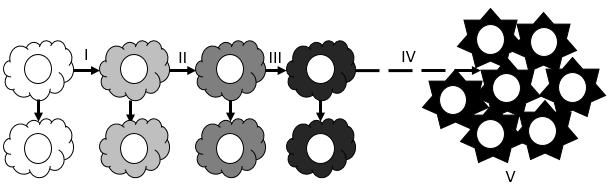
\includegraphics{img/fig-evolution.png}}
\end{center}\vspace*{-0.6cm}
\caption[Proceso de acumulaci\'on de mutaciones que provocan la aparici\'on del c\'ancer]{Proceso de acumulaci\'on de mutaciones que provocan la aparici\'on del c\'ancer~\cite{robins}. Las mutaciones sufridas por las poblaciones de c\'elulas y sus descendientes son las siguientes: aparece una mutaci\'on inicial que desactiva un inhibidor del ciclo celular~(\emph{I}); la c\'elula mutada contin\'ua su divisi\'on y un descendiente adquiere una nueva mutaci\'on que activa un estimulante del ciclo celular~(\emph{II}); el proceso contin\'ua y aparece una c\'elula con una nueva mutaci\'on que desactiva un factor de estabilidad gen\'omico~(\emph{III}); las mutaciones se acumulan r\'apidamente por la p\'erdida de la estabilidad gen\'etica hasta que aparece la primera c\'elula cancer\'igena~(\emph{IV}); aparece el c\'ancer como enfermedad por la divisi\'on descontrolada de estas c\'elulas altamente mutadas~(\emph{V}).}
\label{fig-evolution}
\end{figure}

\section{Inmortalidad replicativa}
\label{subsec-inm-rep}
Todos los organismos tienen formas y tama\~nos definidos, tanto a nivel celular como a nivel de tejidos. Casi todos los tipos de c\'elulas del organismo poseen un conjunto de se\~nales y mecanismos que controlan su ritmo de proliferaci\'on. Este control es vital para mantener la integridad de las c\'elulas y el tejido. Si las c\'elulas se dividieran de forma descontrolada sin ning\'un tipo de restricci\'on, los tejidos podr\'ian desarrollarse hasta alcanzar tama\~nos enormes con resultados letales para el organismo~\cite{hanahan}.

Las c\'elulas cancer\'igenas se definen t\'ipicamente por su capacidad de dividirse sin control alguno. Para que un peque\~no conjunto de c\'elulas clonales se expandan hasta el tama\~no de un tumor potencialmente fatal debe existir un trastorno en los mecanismos celulares que controlan su divisi\'on. En un cultivo las c\'elulas normales pueden llevar a cabo una cantidad finita de divisiones antes de que detengan su divisi\'on completamente, mientras que las c\'elulas cancer\'igenas pueden dividirse indefinidamente. Esto ocurre porque las c\'elulas poseen un n\'umero finito de posibles divisiones celulares o potencial replicativo. Una c\'elula humana puede dividirse de 60 a 70 veces como promedio antes de que incurra en un proceso conocido como senescencia. Una c\'elula senescente es viable pero ha perdido su capacidad de dividirse. Un ejemplo de la inmortalidad replicativa de las c\'elulas cancer\'igenas son las c\'elulas HeLa. Estas c\'elulas fueron cultivadas de un adenocarcinoma cervical de un paciente de c\'ancer llamado Henrietta Lacks en 1951, y hasta el d\'ia de hoy estas c\'elulas contin\'uan su crecimiento y proliferaci\'on en cientos de laboratorios alrededor del mundo. Esto sugiere claramente que estas c\'elulas cancer\'igenas han interrumpido los mecanismos de senescencia en el interior de la c\'elula ganando un potencial replicativo ilimitado~\cite{robins,hanahan,cancerbook}.

El mecanismo que se encarga de la senescencia es un contador que controla la cantidad finita de divisiones celulares y se encuentra en los extremos de todos los cromosomas del cuerpo humano: los tel\'omeros. Los tel\'omeros son secuencias de material gen\'etico que no codifican ninguna prote\'ina por lo que se conoce como secuencias basura. No obstante, juegan un papel fundamental en la protecci\'on de los cromosomas. Su importancia radica en un problema \'unico presente en la replicaci\'on del c\'odigo gen\'etico durante la divisi\'on celular. Despu\'es de cada ronda de replicaci\'on del c\'odigo gen\'etico se pierde una corta secuencia del tel\'omero en los extremos de cada cromosoma. Como resultado de la degradaci\'on de los tel\'omeros los cromosomas se hacen m\'as cortos. Los ciclos sucesivos de replicaci\'on traen como consecuencia una erosi\'on continua de los tel\'omeros hasta el punto en que comienzan a causar problemas en el c\'odigo gen\'etico tales como cambios gen\'eticos, errores de escritura y muerte celular. Por tanto, una c\'elula normal posee un ciclo vital finito, dictado por la longitud de sus tel\'omeros~(Fig.\ref{fig-telomero})~\cite{robins,hanahan,cancerbook}.

\begin{figure}[!ht]
\begin{center}
\scalebox{0.75}{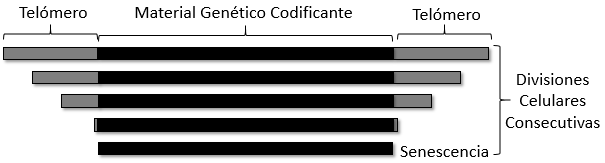
\includegraphics{img/fig-telomero.png}}
\end{center}\vspace*{-0.6cm}
\caption[Proceso de degradaci\'on de los tel\'omeros de una c\'elula]{Proceso de degradaci\'on de los tel\'omeros de una c\'elula a medida que ocurren divisiones celulares consecutivas hasta alcanzar el estado de senescencia.}
\label{fig-telomero}
\end{figure}

Las c\'elulas cancer\'igenas por otra parte, mantienen la longitud de sus te\-l\'omeros sin la p\'erdida de material gen\'etico codificante. La principal estrategia utilizada para mantener la longitud de los tel\'omeros es mediante la activaci\'on de una enzima llamada telomerasa. El $85$-$90\%$ de todas las formas de c\'ancer presentan la activaci\'on de telomerasa. La telomerasa mantiene la longitud de los tel\'omeros por encima del umbral cr\'itico, previniendo la erosi\'on y habilitando un potencial replicativo ilimitado~\cite{robins,hanahan,cancerbook}.

La evidencia listada sugiere que la senescencia es un mecanismo de protecci\'on utilizado por las c\'elulas para entrar en una fase inactiva que detiene su proliferaci\'on. Los tumores evitan la senescencia activando la telomerasa por lo que las estrategias terap\'euticas encaminadas a inhibir la telomerasa afectar\'a preferentemente a c\'elulas cancer\'igenas y no al correcto funcionamiento del organismo. 

\section{Oncogenes}
\label{subsec-oncogene}
Las c\'elulas no pueden sobrevivir en aislamiento. Las c\'elulas forman parte de un tejido o \'organo y su comportamiento casi siempre depende de se\~nales de crecimiento provenientes del entorno que activan la divisi\'on celular. Estas se\~nales de crecimiento se adhieren a la c\'elula y promueven o inhiben la expresi\'on de genes espec\'ificos. Entre las se\~nales de crecimiento est\'an los factores de crecimiento, las prote\'inas de la matriz extracelular~(de ahora en adelante ECM) y las mol\'eculas de adhesi\'on e interacci\'on intercelular. Si estas se\~nales est\'an ausentes una c\'elula normal entrar\'ia en un estado inactivo y no llevar\'ia a cabo divisiones celulares activas. Esta dependencia de se\~nales de crecimiento externas es un mecanismo cr\'itico para controlar el comportamiento de las c\'elulas que conforman un tejido~\cite{robins,hanahan,cancerbook}. 

Las c\'elulas cancer\'igenas por otra parte, generan prote\'inas mutantes~(prote\'inas oncog\'enicas) que imitan las se\~nales de crecimiento normales~(prote\'inas protooncog\'enicas). La transformaci\'on de protooncogenes en oncogenes puede ser el resultado de numerosos factores como mutaciones, reorganizaciones cromos\'omicas, amplificaciones de genes entre otras. La consecuencia de la transformaci\'on oncog\'enica es que las c\'elulas del tumor se vuelven independientes de estas se\~nales externas de crecimiento. Esta habilidad adquirida por las c\'elulas tumorales puede ser demostrada de forma emp\'irica en cultivos \textit{in vitro}~\cite{robins,hanahan,cancerbook}.

Las c\'elulas normales que han sido cultivadas \textit{in vitro} no se dividen y no proliferan en ausencia de factores de crecimiento en el medio de cultivo. Las c\'elulas tumorales en cambio pueden proliferar activamente sin depender de estos factores. Pueden adem\'as crear sus propios factores mediante mutaciones en los mecanismos de fabricaci\'on haciendo que est\'en siempre activas e ignoren las se\~nales que interrumpen su funcionamiento. En \'ultima instancia pueden inducir la producci\'on de estos factores en las c\'elulas vecinas sanas para suplir su demanda~(Fig.\ref{fig-growth-factor}). Esta autonom\'ia de los factores de crecimiento conlleva a una proliferaci\'on descontrolada e incrementa las probabilidades de adquirir nuevas mutaciones en el c\'odigo gen\'etico~\cite{robins,hanahan,cancerbook}.

\begin{figure}[!ht]
\begin{center}
\scalebox{0.65}{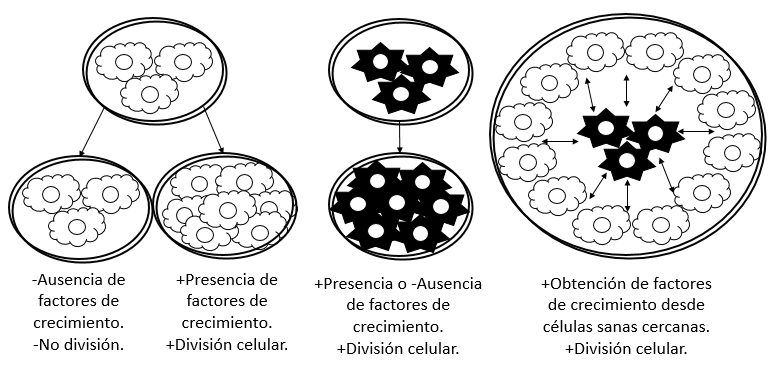
\includegraphics{img/fig-growth-factor.png}}
\end{center}\vspace*{-0.6cm}
\caption[Representaci\'on de las distintas mutaciones que sufren las c\'elulas cancer\'igenas que modifican su respuesta ante la presencia o no de factores de crecimiento, en comparaci\'on con las c\'elulas sanas]{Representaci\'on de las distintas mutaciones que sufren las c\'elulas cancer\'igenas que modifican su respuesta ante la presencia o no de factores de crecimiento, en comparaci\'on con las c\'elulas sanas~\cite{robins}.}
\label{fig-growth-factor}
\end{figure}

\section{Genes supresores de tumores}
\label{subsec-supp-genes}
El balance entre la proliferaci\'on y la inactividad celular es el resultado de una compleja interacci\'on entre los reguladores del ciclo celular: los estimulantes y los inhibidores. Como apreciamos anteriormente, los estimulantes comprenden una variedad de se\~nales y factores de crecimiento que activan la proliferaci\'on celular. Sin embargo, los tejidos sanos tambi\'en est\'an sujetos a se\~nales antiproliferaci\'on que son responsables de la inactividad celular, y act\'uan como frenos a las se\~nales de crecimiento. Los inhibidores pueden estar presentes en la ECM y en la superficie celular~\cite{robins,hanahan,cancerbook}. 

De forma similar a las se\~nales de crecimiento, las se\~nales que bloquean o suprimen la divisi\'on celular se reciben a trav\'es de receptores en la superficie de la c\'elula y promueven o inhiben la expresi\'on de genes espec\'ificos. Los genes que codifican esta clase de prote\'inas involucradas en la supresi\'on de la divisi\'on celular se conocen como genes supresores de tumores. Las c\'elulas normales, antes de la divisi\'on celular, verifican constantemente su medio interno y externo para asegurarse de que las condiciones son ideales para la mitosis~(reparto equitativo del material hereditario caracter\'istico). Las se\~nales provenientes del medio externo o interno dictan si la c\'elula deber\'ia dividirse, volverse inactiva o destruirse. Este mecanismo constituye una forma de mantener la homeostasis en el organismo, asegur\'andose que las c\'elulas se dividan en el momento justo y bajo condiciones \'optimas~\cite{robins,hanahan,cancerbook}.

Las c\'elulas cancer\'igenas por otra parte desv\'ian o evaden estas se\~nales de no proliferaci\'on para habilitar su propio crecimiento. Por ejemplo, las mutaciones en los genes que codifican inhibidores del ciclo celular podr\'ian resultar en una divisi\'on celular incrementada. Los genes supresores de tumores constituyen un grupo grande de genes que codifican prote\'inas cuyo rol fundamental es la restricci\'on del ciclo celular. Las mutaciones en estos genes pueden traer como consecuencia una p\'erdida de funcionalidad~\cite{robins,hanahan,cancerbook}.

\section{Apoptosis}
\label{subsec-apopt}
Las c\'elulas verifican constantemente su estado interno incluyendo su acceso a nutrientes y ox\'igeno, la integridad de su genoma y el balance entre los reguladores del ciclo celular. Si esta revisi\'on detecta alg\'un da\~no o mal funcionamiento, se activan sistemas de respaldo que determina si la c\'elula deber\'ia interrumpir su proliferaci\'on y llevar a cabo labores de reparaci\'on o si el da\~no es severo si deber\'ia llevar a cabo la muerte celular. El desarrollo de tumores puede ser visto no como una simple proliferaci\'on excesiva, sino tambi\'en como una reducci\'on en las muertes celulares. La muerte celular programada o apoptosis representa una parte importante en esta hip\'otesis. Existe evidencia en aumento que sugiere que la evasi\'on o resistencia a la apoptosis es una caracter\'istica distintiva de casi todas las formas de c\'ancer~\cite{robins,hanahan,cancerbook}.

La muerte celular programada es parte del desarrollo y crecimiento normales. La homeostasis del tejido es un balance entre las divisiones y muertes celulares, donde la cantidad de c\'elulas que conforman el tejido se mantiene relativamente constante. Si este equilibrio se perturba puede llevar a que las c\'elulas se dividan m\'as r\'apido de lo que mueren, resultando en el desarrollo del c\'ancer o mueran m\'as r\'apido de lo que pueden dividirse, resultando en una atrofia del tejido. La desregulaci\'on de esta compleja homeostasis del tejido se encuentra implicada en muchas formas de c\'ancer.

Las se\~nales de apoptosis pueden provenir del interior de la c\'elula como del medio externo, y activan la muerte celular de forma muy precisa y coordinada. Los principales componentes de estas se\~nales pueden dividirse en dos partes: la primera es la detecci\'on de la se\~nal de apoptosis y la segunda es la ejecuci\'on de la se\~nal. La c\'elula verifica los medios interno y externo para detectar cambios en las condiciones del entorno que puedan influir en su ciclo celular. Entre las se\~nales del medio externo que pueden causar la apoptosis se encuentran la exposici\'on a toxinas y a ciertas hormonas. Las se\~nales internas dependen de si existe o no da\~no en el material gen\'etico o la c\'elula est\'a sujeta a condiciones de estr\'es que pueden afectarla f\'isicamente. Entre estos factores internos se encuentran el calor, la radiaci\'on, la falta de ox\'igeno, la insuficiencia de factores de crecimiento, infecciones virales o un incremento del calcio en el interior de la c\'elula. Es aceptado actualmente que sin importar el origen de la se\~nal, ambas activan mecanismos comunes encargados de llevar a cabo la muerte celular programada~\cite{robins,hanahan,cancerbook}.

Las c\'elulas cancer\'igenas pueden afectar los mecanismos de la apoptosis de muchas maneras, pero el m\'etodo m\'as com\'un involucra mutaciones del gen supresor de tumores \textit{p53}. La funci\'on principal del gen \textit{p53} es la de detectar da\~nos en el c\'odigo gen\'etico y determinar el curso de acci\'on. Si el da\~no es reparable el gen \textit{p53} induce labores de reparaci\'on en el c\'odigo gen\'etico, pero si el da\~no es irreparable, entonces es el encargado de enviar una se\~nal para llevar a cabo la apoptosis. M\'as del $50\%$ de todas las formas de c\'ancer del ser humano y el $80\%$ de los carcinomas de c\'elulas escamosas muestran una inactivaci\'on de este gen~(Fig.\ref{fig-apoptosis}). Este es el ejemplo m\'as com\'un, pero en la c\'elula existen una mayor cantidad de mecanismos de detecci\'on de se\~nales de muerte celular y ejecuci\'on de dicha se\~nal. Es improbable que una forma dada de c\'ancer haya perdido todos los mecanismos relacionados con la apoptosis. La identificaci\'on de los mecanismos que retienen su funcionalidad constituye una v\'ia de combatir la enfermedad mediante el dise\~no de drogas que tengan como objetivo su activaci\'on~\cite{robins,hanahan,cancerbook}.

\begin{figure}[!ht]
\begin{center}
\scalebox{0.65}{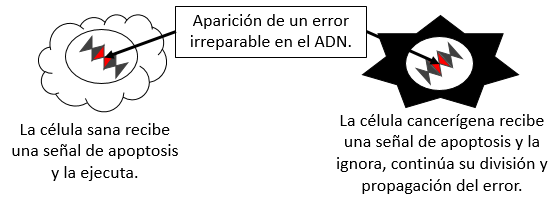
\includegraphics{img/fig-apoptosis.png}}
\end{center}\vspace*{-0.6cm}
\caption[Representaci\'on del proceso de apoptosis en una c\'elula sana y una cancer\'igena ante la aparici\'on de un error en el c\'odigo gen\'etico]{Representaci\'on del proceso de apoptosis en una c\'elula sana y una cancer\'igena ante la aparici\'on de un error en el c\'odigo gen\'etico~\cite{robins}.}
\label{fig-apoptosis}
\end{figure}

Es evidente que los cambios en los mecanismos que llevan a cabo la apoptosis pueden afectar dram\'aticamente la din\'amica de la progresi\'on tumoral, haciendo de estos cambios un factor clave para el desarrollo del c\'ancer. 

\section{Angiog\'enesis}
\label{subsec-angio}
Las c\'elulas y los tejidos necesitan ox\'igeno y nutrientes para sobrevivir y proliferar por lo que la mayor\'ia de las c\'elulas yacen a menos de $0$.$1mm$ de un capilar sangu\'ineo. Bajo la mayor\'ia de las circunstancias las c\'elulas que conforman el endotelio, tejido que recubre la zona interna de todos los vasos sangu\'ineos y el coraz\'on, no se dividen ni crecen. Sin embargo, bajo ciertas situaciones como la sanaci\'on de una herida, se activa la divisi\'on de las c\'elulas endoteliales provocando el crecimiento de nuevos capilares sangu\'ineos. Este proceso se conoce como angiog\'enesis o neovascularizaci\'on.

Los tumores tienen la capacidad de inducir la angiog\'enesis y constituye un paso fundamental en la transici\'on de un grupo peque\~no de c\'elulas mutadas~(tumor \textit{in situ}) en un crecimiento maligno capaz de invadir los tejidos vecinos y \'organos distantes. Esta transici\'on puede tomar muchos meses o a\~nos, y a menos que se induzca la angiog\'enesis, los tumores s\'olidos no crecer\'an m\'as de $1$-$2mm$. Como ocurre con la mayor\'ia de los mecanismos que mantienen la homeostasis celular, la angiog\'enesis tambi\'en comprende un balance entre se\~nales positivas y negativas que estimulan o inhiben este proceso. Se conoce que la habilidad para inducir y mantener la angiog\'enesis se adquiere en una serie de pasos discretos durante el desarrollo tumoral. Se muestra a continuaci\'on una revisi\'on simplificada de este proceso~\cite{robins,hanahan,cancerbook}:

\begin{enumerate}
\item [I.] El tumor libera factores angiog\'enicos que se difunden en los tejidos cercanos y se acoplan a receptores en las c\'elulas endoteliales de los vasos sangu\'ineos preexistentes, provocando su activaci\'on.

\item [II.] Tales interacciones entre las c\'elulas tumorales y las endoteliales conlleva a la secreci\'on y activaci\'on de enzimas que degradan la membrana basal y la matriz extracelular.

\item [III.] La degradaci\'on de la membrana basal permite que las c\'elulas endoteliales activas migren hacia el tumor.

\item [IV.] Las c\'elulas endoteliales depositan una nueva membrana basal y secretan factores de crecimiento que atraen a c\'elulas de soporte de la matriz extracelular para que estabilicen el nuevo vaso sangu\'ineo.
\end{enumerate}

Sin embargo, todav\'ia no se comprenden por completo los mecanismos que afectan el balance angiog\'enico a favor del tumor. El escenario m\'as probable es que existan relaciones entre estos mecanismos de balance y otros reguladores de la homeostasis celular. Por ejemplo, el gen supresor de tumores \textit{p53} se encuentra estrechamente relacionado con un inhibidor angiog\'enico. Por tanto, cualquier afectaci\'on al normal funcionamiento del gen \textit{p53}, que es com\'un en el desarrollo tumoral, puede causar una ca\'ida en los niveles del inhibidor provocando un desbalance angiog\'enico~\cite{robins,hanahan,cancerbook}.

La angiog\'enesis tumoral constituye un blanco irresistible para el desarrollo de terapias que afecten el desarrollo tumoral. En la actualidad los tratamientos antiangiog\'enicos constituyen una fracci\'on numerosa de los ensayos cl\'inicos que se est\'an llevando a cabo para combatir el c\'ancer.

\section{Met\'astasis}
\label{subsec-meta}
Los tumores s\'olidos, bajo condiciones \'optimas, pueden invadir los tejidos locales y atravesar el sistema circulatorio para colonizar \'organos y tejidos distantes. Estos tumores secundarios son responsables de casi el $90\%$ de las muertes relacionadas con el c\'ancer. La capacidad de las c\'elulas tumorales de invadir y colonizar es la sexta marca distintiva del c\'ancer. Seg\'un~\cite{robins,hanahan}, las definiciones de los t\'erminos \textit{invasi\'on local} y \textit{met\'astasis} son:

\paragraph{Invasi\'on local:}El crecimiento del c\'ancer se acompa\~na de una infiltraci\'on, invasi\'on y destrucci\'on progresivas del tejido circundante, mostrando un rompimiento de la membrana basal. Adem\'as de las met\'astasis, la capacidad de invasi\'on es el rasgo m\'as fiable para distinguir el c\'ancer de los tumores benignos.

\paragraph{Met\'astasis:}Se define como la propagaci\'on del tumor a sitios f\'isicamente alejados del tumor primario y marca, de un modo inequ\'ivoco, dicho tumor como maligno ya que por definici\'on, una neoplasia benigna no metastatiza.\vspace*{0.5cm}

Una vez que un tumor infiltra satisfactoriamente los tejidos vecinos sanos, las c\'elulas cancer\'igenas que lo conforman sufren distintas transformaciones que provocan la p\'erdida de la capacidad de adhesi\'on celular y cambios en la matriz de interacci\'on intercelular~\cite{hanahan,invasion}. La disminuci\'on de la adhesi\'on celular permite que ocurran desprendimientos de c\'elulas cancer\'igenas pertenecientes al tumor primario. Estas c\'elulas sufren cambios en la matriz de interacci\'on celular que provocan la expresi\'on de prote\'inas involucradas en el control de la movilidad, la supresi\'on de reguladores de la migraci\'on y la degradaci\'on de la ECM y la membrana basal. De esta forma pueden migrar a trav\'es del tejido circundante y adaptarse r\'apidamente para vencer numerosas dificultades que presentan los nuevos entornos~\cite{hanahan,invasion}. Estas c\'elulas tambi\'en son la causa fundamental de las recurrencias cuando la masa principal del tumor es removida quir\'urgicamente~\cite{kansal3}. 

Las c\'elulas cancer\'igenas muestran una variedad de estrategias de migraci\'on y pueden alternar entre ellas para hacerle frente a entornos hostiles~\cite{migration}. Los factores determinantes en el proceso de migraci\'on son la expresi\'on de mecanismos de uni\'on intercelulares y los cambios de la estructura de las c\'elulas invasivas. La invasi\'on individual puede ser llevada a cabo por c\'elulas con estructuras espigadas, elongadas y redondeadas~\cite{migration} que degradan la matriz extracelular y se mueven a trav\'es de ella. La invasi\'on colectiva puede darse en forma de conjuntos migrantes que se desprenden del tumor o formando largas cadenas invasivas que parten desde el mismo~\cite{robins,hanahan,cancerbook}.

Eventualmente las c\'elulas migrantes entran en contacto con el sistema circulatorio, ya sea con capilares sangu\'ineos o vasos linf\'aticos. En este punto pueden penetrar dicho sistema, viajar en su interior hasta encontrar una localizaci\'on favorable para abandonarlo y colonizar el tejido circundante. A este proceso se le conoce como met\'astasis y los pasos que la comprenden constituyen la cascada metast\'asica: invasi\'on local, migraci\'on, penetraci\'on del sistema circulatorio~(\textit{intravasation}), transporte, abandono del sistema circulatorio~(\textit{extravasation}), formaci\'on de micromet\'astasis y colonizaci\'on~\cite{robins,invasion,hanahan,cancerbook}. Una vez el tumor primario ha comenzado el proceso de angiog\'enesis, si bien las c\'elulas cancer\'igenas deben tener las caracter\'isticas necesarias para efectuar la invasi\'on local, pueden acceder al sistema circulatorio desde los reci\'en formados capilares sangu\'ineos que sustentan al tumor, sin la necesidad de penetrar los tejidos vecinos.

Las mutaciones necesarias para que las c\'elulas cancer\'igenas sean capaces de efectuar la invasi\'on local y la met\'astasis son comunes para ambos procesos. Sin embargo, para la colonizaci\'on satisfactoria de un \'organo distante estas c\'elulas deben poseer una mayor resistencia. El proceso de met\'astasis es altamente ineficiente~\cite{pubmed}, ya que la cantidad de c\'elulas que dejan el tumor primario son del orden de los millones en un d\'ia, pero solo una peque\~na fracci\'on de las mismas son capaces de sobrevivir a la cascada metast\'asica. Las c\'elulas migratorias pueden terminar su existencia por una gran variedad de causas, entre las que se encuentran:

\begin{itemize}
\item Una c\'elula sobrevive normalmente conectada a sus vecinos y al conjunto de prote\'inas existente a su alrededor. El desprendimiento de la superficie de otras c\'elulas puede llevar a la muerte celular.
\item Las c\'elulas cancer\'igenas son con frecuencia mucho mayores en tama\~no que las c\'elulas que viven en el sistema circulatorio. Cuando estas viajan a trav\'es de dicho sistema pueden da\~narse o atascarse, llevando a la muerte celular.
\item Las c\'elulas cancer\'igenas pueden ser reconocidas y destruidas por c\'elulas del sistema inmunitario.
\end{itemize}

A\'un cuando una c\'elula metast\'asica sobrevive todo el proceso, esto no significa que forme un tumor secundario satisfactoriamente. Dicha c\'elula debe crear un entorno favorable dentro de un nuevo ambiente hostil que les permita sobrevivir y crecer. Esta capacidad de transformar el entorno es un hecho crucial como lo demuestran numerosos experimentos~\cite{pubmed}. En un estudio experimental de un melanoma metast\'asico, m\'as del $80\%$ de las c\'elulas cancer\'igenas sobrevivieron al transporte a trav\'es del sistema circulatorio y arribaron al h\'igado. De estas, solamente $1$ c\'elula de cada $40$ formaron micromet\'astasis en un lapso de $3$ d\'ias, y $1$ de cada $100$ formaron macromet\'astasis en $10$ d\'ias. La tarea de crear un entorno favorable parece ser un proceso complejo que limita notablemente la capacidad de la c\'elula de formar un tumor secundario. Cuando una c\'elula cancer\'igena entra en contacto con un nuevo \'organo, puede ocurrir una de tres variantes:

\begin{itemize}
\item El tejido circundante del nuevo \'organo puede ser muy diferente de donde se origin\'o el tumor primario, y en la mayor\'ia de los casos puede ser muy hostil, al punto de impedir la supervivencia de la c\'elula cancer\'igena, llevando a su muerte celular. 
\item Si dicha c\'elula metast\'asica no posee la capacidad de transformar el tejido en un entorno m\'as amistoso, no podr\'a colonizar satisfactoriamente. En este caso se dice que la c\'elula entra en un per\'iodo de dormancia, no muere, pero no es capaz de crecer. Ocasionalmente dichas micromet\'astasis latentes obtienen nuevas mutaciones que les permite colonizar satisfactoriamente dicho \'organo.
\item La c\'elula migrante posee todas las capacidades necesarias para colonizar la nueva localizaci\'on, como se ha comprobado en tumores que hacen met\'astasis en el mismo \'organo donde surgi\'o el tumor primario, o en \'organos espec\'ificos. Distintos tipos de c\'ancer tienen preferencia por \'organos espec\'ificos para ser atacados por c\'elulas migratorias~\cite{invasion}.
\end{itemize}

Precisamente la tendencia de colonizar \'organos espec\'ificos seg\'un los diferentes tipos de c\'ancer se conoce como la hip\'otesis de la semilla y el sustrato~(\textit{the seed and soil hypothesis})~\cite{paget}. En 1889 Stephen Paget observ\'o que los pacientes con c\'ancer de mama desarrollaban tumores secundarios en el h\'igado con frecuencia. Consider\'o que era poco probable que esto sucediese principalmente por la accesibilidad del h\'igado al sistema circulatorio, ya que otros \'organos que poseen un acceso al suministro de sangre equivalente desarrollaban met\'astasis muy rara vez. En base a esto, desarroll\'o dicha hip\'otesis, en la cual ciertas c\'elulas cancer\'igenas solo pueden colonizar satisfactoriamente \'organos selectos que poseen entornos de crecimiento adecuados o deseables~\cite{paget,metastasis}, entre los que se incluye el entorno del \'organo primario. Esta hip\'otesis comprende tres conceptos importantes:

\begin{itemize}
\item Los tumores primarios y sus met\'astasis est\'an compuestos de c\'elulas tumorales gen\'eticamente muy diversas.
\item Las c\'elulas seleccionadas para llevar a cabo la met\'astasis son las que pueden sobrevivir a toda la cascada.
\item Las c\'elulas seleccionadas colonizan una localizaci\'on en una forma muy espec\'ifica, y dado que los entornos de cada \'organo son distintos las c\'elulas cancer\'igenas solo podr\'an colonizar un tipo de \'organo espec\'ifico.
\end{itemize}

Estos conceptos muestran la idea de que una met\'astasis satisfactoria depende completamente de las interacciones entre las c\'elulas cancer\'igenas y las c\'elulas del \'organo objetivo. Estas c\'elulas que reci\'en est\'an formando una nueva met\'astasis no solo tienen que ser capaces de producir los factores requeridos por ellas para sobrevivir y crecer en el nuevo entorno, sino que el entorno del nuevo \'organo tiene que ser capaz de responder a estas se\~nales y actuar en consecuencia. Si la c\'elula cancer\'igena se encuentra en un entorno muy inh\'ospito ser\'a imposible que una met\'astasis se forme satisfactoriamente~\cite{metastasis}. Si una c\'elula cancer\'igena sobrevive al transporte en el interior del sistema circulatorio y lleva a cabo la extravasaci\'on de forma satisfactoria puede ocurrir una de tres situaciones~\cite{circulating}:

\begin{itemize}
\item La extravasaci\'on de la c\'elula ocurre en la localizaci\'on del tumor donde se origin\'o, es decir, penetr\'o el sistema circulatorio, sobrevivi\'o a su transporte y arrib\'o al propio punto de origen. En este caso contribuye a la poblaci\'on tumoral en la localizaci\'on primaria.
\item La extravasaci\'on de la c\'elula ocurre en la localizaci\'on de una met\'astasis. En este caso se comporta de igual forma, contribuyendo con la poblaci\'on tumoral.
\item La extravasaci\'on de la c\'elula ocurre en una localizaci\'on no colonizada a\'un. En este caso puede asentarse y comenzar una nueva met\'astasis.
\end{itemize}

\section{Evoluci\'on macrosc\'opica del c\'ancer}
\label{subsec-macro}
La c\'elula cancer\'igena a medida que acumula mutaciones adquiere nuevas capacidades que alteran el comportamiento del tumor. La obtenci\'on de las seis mutaciones distintivas provocan los cambios m\'as evidentes y proveen de un modelo ideal para describir su progresi\'on macrosc\'opica y las transiciones entre las distintas etapas. Para ilustrar este proceso se utiliza como referencia el grupo de neoplasias conocidas como carcinomas que representan el $80\%$ de los tumores malignos. Estos tienen su origen en el epitelio, tejido que recubre gran parte del organismo como el revestimiento interno de las cavidades, \'organos huecos, conductos, mucosas, gl\'andulas y en muchos casos constituyen el tejido funcional. Se trata de capas de c\'elulas fuertemente enlazadas que descansan sobre una membrana basal, separ\'andolas del tejido de sost\'en subyacente. El epitelio carece de vasos sangu\'ineos por lo que su sustento depende de la difusi\'on de nutrientes a trav\'es de la membrana basal provenientes de los capilares sangu\'ineos presentes en el tejido de sost\'en~(Fig.\ref{fig-epitelium}).

\begin{figure}[!ht]
\begin{center}
\scalebox{0.75}{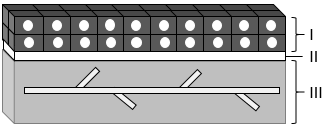
\includegraphics{img/fig-epitelium.png}}
\end{center}\vspace*{-0.6cm}
\caption[Distribuci\'on del tejido epitelial, la membrana basal y el tejido de sost\'en subyacente]{Distribuci\'on del tejido epitelial~(I), la membrana basal~(II) y el tejido de sost\'en subyacente~(III). Se observa la vasculatura del tejido de sost\'en.}
\label{fig-epitelium}
\end{figure}

El desarrollo de una neoplasia maligna se divide en dos etapas principales: la etapa celular y la etapa macrosc\'opica. La primera se refiere a la evoluci\'on temprana del tumor, cuando las c\'elulas proliferantes no han comenzado a aglomerarse. La segunda comienza cuando agrupaciones de estas c\'elulas proliferantes se condensan en una forma compacta. El cambio m\'as notable durante la evoluci\'on macrosc\'opica es el relacionado con el proceso de angiog\'enesis que hace que el tumor aumente r\'apida y considerablemente de tama\~no. Por este hecho se usa la vascularizaci\'on como l\'inea divisoria entre las etapas macrosc\'opicas~\cite{vascular}. 

La etapa avascular se caracteriza por un desarrollo local de la neoplasia, con un rango de acci\'on y peligrosidad limitadas, en el que las c\'elulas tumorales presentan un alto grado de adhesi\'on, haciendo del tumor una masa compacta con forma semiesf\'erica~\cite{ruben,vascular}. La difusi\'on de los nutrientes y el ox\'igeno transportados por el sistema circulatorio constituye la forma de sustento principal del tumor. En diversos estudios \textit{in vitro} se han utilizado MTS para simular el desarrollo avascular tumoral. Estos exhiben una proliferaci\'on exponencial inicial seguida de una saturaci\'on en el crecimiento, incluso en presencia de un suministro constante de nutrientes. Los procesos responsables de este comportamiento se relacionan con la auto organizaci\'on de las c\'elulas tumorales y el alcance limitado de la difusi\'on~\cite{kansal,dormann}. Se puede inferir que sin una nueva forma de obtener los nutrientes el tumor no puede crecer por encima de $1$ o $2mm$. Durante esta etapa las c\'elulas cancer\'igenas presentan en alguna medida las mutaciones distintivas relacionadas directamente con el ciclo celular: la inmortalidad replicativa, la producci\'on de se\~nales de crecimiento, la evasi\'on de se\~nales que inhiben su proliferaci\'on y la resistencia a la muerte celular. A medida que progresa esta etapa, dichas mutaciones se vuelven m\'as marcadas aumentando la malignidad del tumor~\cite{vascular}. A pesar de esto, rara vez muestran signos de invasi\'on local, confin\'andose al tejido donde se origin\'o la neoplasia, lo que se conoce como tumor \textit{in situ}~(Fig.\ref{fig-epitelium-2}).

\begin{figure}[!ht]
\begin{center}
\scalebox{0.5}{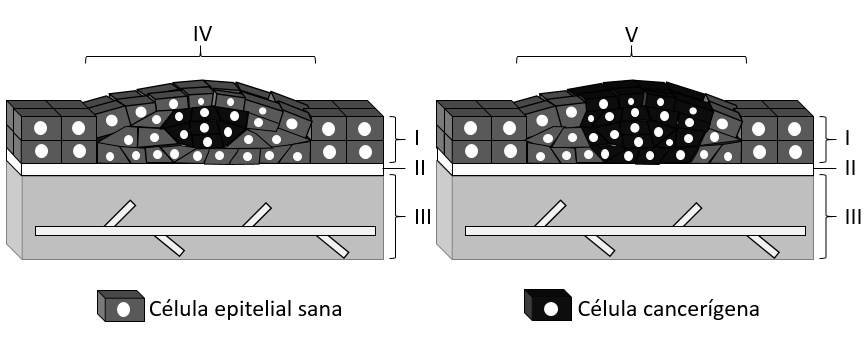
\includegraphics{img/fig-epitelium-2-horizontal.png}}
\end{center}\vspace*{-1cm}
\caption[Evoluci\'on de un tumor durante la etapa avascular]{Evoluci\'on de un tumor durante la etapa avascular. Se aprecia en ambos esquemas el desplazamiento de las c\'elulas sanas del epitelio~(\emph{I}) por la expansi\'on del tumor~(\emph{IV}, \emph{V}). Eventualmente la lesi\'on se vuelve visible en la cavidad~(\emph{V}) pues las c\'elulas cancer\'igenas se alzan sobre el epitelio. La membrana basal~(\emph{II}) se mantiene intacta y no existe invasi\'on del tejido de sost\'en subyacente~(\emph{III}) por parte del tumor.}
\label{fig-epitelium-2}
\end{figure}

\begin{figure}[!ht]
\begin{center}
\scalebox{0.5}{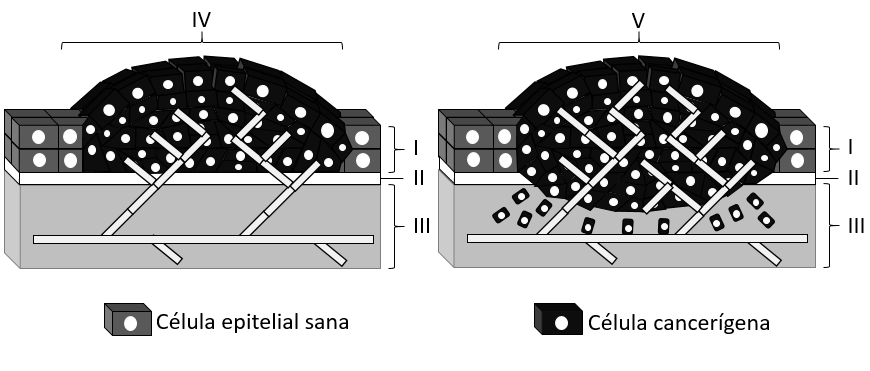
\includegraphics{img/fig-epitelium-3-horizontal.png}}
\end{center}\vspace*{-1cm}
\caption[Evoluci\'on de un tumor durante la etapa vascular]{Evoluci\'on de un tumor durante la etapa vascular. Se aprecia en ambos esquemas el incremento de la neovasculatura inducida por el tumor~(\emph{IV}, \emph{V}). En un principio las c\'elulas cancer\'igenas~(\emph{IV}) no son capaces de penetrar la membrana basal~(\emph{II}). Pero el progreso de la angiog\'enesis degrada esta membrana~(\emph{II}) permitiendo la invasi\'on~(\emph{V}) del tejido de sost\'en subyacente~(\emph{III}). En los instantes de m\'aximo desarrollo de la neoplasia ocurren desprendimientos de c\'elulas que proceden a continuar la cascada metast\'asica~(\emph{V}).}
\label{fig-epitelium-3}
\end{figure}

Una vez que el tumor alcanza el m\'aximo tama\~no sostenible mediante la difusi\'on de nutrientes, comienza su entrada en la etapa vascular. El evento que define la transici\'on de una etapa a la otra es la adquisici\'on, por parte de las c\'elulas cancer\'igenas, de la capacidad de producir factores angiog\'enicos que penetran el tejido sano circundante y estimulan el crecimiento de nuevos vasos sangu\'ineos~\cite{robins,vascular}. Estos vasos reci\'en formados penetran la masa del tumor aliment\'andolo con abundantes nutrientes y potenciando su crecimiento por encima del m\'aximo permitido~\cite{vascular,invasion}. Como consecuencia del proceso de angiog\'enesis y de los cambios en la matriz de interacci\'on de las c\'elulas tumorales ocurre una degradaci\'on de la membrana basal y de la matriz extracelular. Esto posibilita la invasi\'on local de los tejidos vecinos, abandonando la condici\'on de tumor \textit{in situ} para transformarse en un tumor invasivo. Eventualmente las c\'elulas cancer\'igenas cercanas o pertenecientes a la frontera del tumor sufren de la p\'erdida de la adhesi\'on intercelular y comienzan a expresar movilidad. De esta forma pueden desprenderse y migrar a trav\'es del tejido de sost\'en hasta alcanzar un capilar o vaso sangu\'ineo, con el objetivo de continuar y culminar la cascada metast\'asica~(Fig.\ref{fig-epitelium-3}).


\newpage
\chapter{Definici\'on del modelo}
\label{sec-ca}
En esta secci\'on se concibe el modelo de aut\'omatas celulares que se presenta en este trabajo. Se comienza definiendo formalmente un aut\'omata celular~\cite[p\'agina 67]{book}.

\begin{definition}
\label{def-automata}
Un aut\'omata celular es una tupla $(\mathcal{L}; \mathcal{N}; \mathcal{E}; \mathcal{R})$ que se compone de los siguientes elementos representativos:
\begin{itemize}
\item [$\mathcal{L}$:] Es un conjunto potencialmente infinito de c\'elulas.
\item [$\mathcal{N}$:] $\mathcal{L} \times \mathcal{L} \rightarrow \lbrace 0,1 \rbrace$ es una funci\'on de vecindad, que puede ser vista como una relaci\'on, usualmente reflexiva y sim\'etrica, entre las c\'elulas. Esta funci\'on muestra qu\'e pares de c\'elulas son vecinas, o sea, la geometr\'ia de la organizaci\'on celular.
\item [$\mathcal{E}$:] Es un conjunto de estados. A cada c\'elula del conjunto $\mathcal{L}$ se le asigna un estado asociado en cada instante de tiempo.
\item [$\mathcal{R}$:] $\mathcal{E}^{|\mathcal{N}(v)|} \rightarrow \mathcal{E}$ es una funci\'on de transici\'on definida localmente. Esta funci\'on es el n\'ucleo de la din\'amica de un aut\'omata celular, y com\'unmente se expresa mediante reglas que definen el estado de la c\'elula en el siguiente instante de tiempo a partir del estado de las c\'elulas vecinas. El conjunto que contiene el estado de las c\'elulas vecinas se obtiene mediante la funci\'on $\mathcal{N}(v)$, que se define en~\ref{def-neighbourhood}.
\end{itemize}
\end{definition}

Un problema que surge al consultar la bibliograf\'ia sobre aut\'omatas celulares y modelos que hacen uso de los mismos es la notaci\'on y la formulaci\'on de los conceptos propios del tema. Diferentes autores proponen notaciones distintas para expresar ideas similares y definiciones generales que se adaptan a su problema particular, llevando a cabo una relajaci\'on del rigor matem\'atico. En el presente trabajo se utiliza la notaci\'on empleada en~\cite[p\'aginas 59-101]{book} escrita por Andreas Deutsch y Sabine Dormann, autores de numerosos art\'iculos relacionados con la modelaci\'on matem\'atica y, en especial, la modelaci\'on mediante aut\'omatas celulares.

\section{Hip\'otesis del modelo}
\label{subsec-hipo}
Como se expuso en la secci\'on~\ref{sec-cancer} el c\'ancer es una enfermedad extremadamente compleja compuesta por una gran cantidad de procesos, interacciones celulares y factores. Es parte del proceso de modelaci\'on lograr una simplificaci\'on del problema para hacerlo tratable, mediante la reducci\'on de la realidad a un conjunto de hip\'otesis. A continuaci\'on se plantean las hip\'otesis generales en las que se basa el presente modelo de aut\'omatas celulares, pero en secciones posteriores se expondr\'an suposiciones m\'as espec\'ificas a medida que se profundice en los distintos temas. El modelo toma como objeto de estudio al tipo de c\'ancer conocido como carcinoma o c\'ancer de c\'elulas epiteliales.

\begin{enumerate}
\item [{I.}] \textbf{Progresi\'on idealizada del desarrollo tumoral}: \emph{Se asume que el desarrollo tumoral sigue una progresi\'on idealizada dividida en las etapas avascular y vascular, donde el comportamiento macrosc\'opico del tumor est\'a definido por las mutaciones que expresan las c\'elulas cancer\'igenas.} \label{I}

\item [{II.}] \textbf{Mutaciones de las c\'elulas cancer\'igenas}: \emph{Se asume que la acumulaci\'on de mutaciones en la c\'elula cancer\'igena se define como un proceso secuencial y sigue un orden establecido, es decir, durante la etapa avascular se expresan las mutaciones relacionadas con el ciclo celular y la proliferaci\'on tumoral, y durante la etapa vascular se expresan las mutaciones relacionadas con la angiog\'enesis y met\'astasis, en adici\'on a las anteriores.} \label{II}

\item [{III.}] \textbf{Entidades biol\'ogicas del modelo}: \emph{Las entidades biol\'ogicas presentes en el modelo se componen \'unicamente de los tipos de c\'elulas definidos en el conjunto de estados del aut\'omata celular.} \label{III}

\item [{IV.}] \textbf{Interacciones entre las entidades del modelo}: \emph{Las interacciones entre las distintas c\'elulas del modelo se compone solamente por las reglas definidas en la funci\'on de transici\'on del aut\'omata.} \label{IV}

\item [{V.}] \textbf{Invarianza de las c\'elulas normales}: \emph{Se asume que la poblaci\'on de c\'elulas normales del organismo es est\'atica e invariante durante el transcurso del tiempo, es decir, no incurren en los procesos de divisi\'on ni muerte celular.} \label{V}

\item [{VI.}] \textbf{Homogeneidad de las c\'elulas cancer\'igenas}: \emph{Se asume que la poblaci\'on de c\'elulas cancer\'igenas que conforma la masa de un tumor es homog\'enea, es decir, no existen subtipos con mutaciones distintas o que est\'en en distintas etapas del ciclo celular.} \label{VI}

\item [{VII.}] \textbf{Suficiencia de nutrientes}: \emph{Se asume que el suministro de nutrientes y ox\'igeno es constante y suficiente para que todo tumor representado en el aut\'omata celular se desarrolle adecuadamente.} \label{VII}

\item [{VIII.}] \textbf{Desarrollo tumoral en funci\'on de la poblaci\'on}: \emph{Se asume que el avance de un tumor a trav\'es de las distintas etapas de su desarrollo depende \'unicamente de su poblaci\'on celular, descrita por la ecuaci\'on de Verhulst de crecimiento log\'istico.} \label{VIII}

\item [{IX.}] \textbf{Proceso de crecimiento simple}: \emph{El desarrollo tumoral se representa mediante un proceso de crecimiento simple, es decir, una posici\'on ocupada por una de estas c\'elulas tumorales permanece ocupada en los restantes instantes de tiempo, salvo que la masa cancer\'igena a la que pertenecen sea eliminada de la simulaci\'on como ocurre con las met\'astasis. } \label{IX}

\item [{X.}] \textbf{Adhesi\'on celular}: \emph{Se asume que la adhesi\'on de las c\'elulas tumorales se mantiene en todo momento salvo en los desprendimientos de c\'elulas migratorias como parte de la cascada metast\'asica.} \label{X}

\item [{XI.}] \textbf{V\'ias de la met\'astasis}: \emph{Se consideran solamente la diseminaci\'on hem\'atica y linf\'atica como v\'ias de la met\'astasis.} \label{XI}

\item [{XII.}] \textbf{Representaci\'on del tejido}: \emph{Se asume que un tejido puede ser representado mediante una red de mundo peque\~no, generada a partir del modelo Watts-Strogatz donde las coordenadas de los v\'ertices poseen dos componentes $x,y \in \mathbb{N}$ que constituyen la localizaci\'on de la c\'elula en el plano correspondiente con un corte de dicho tejido.} \label{XII}
\end{enumerate}

Esta \'ultima hip\'otesis es la que permite asumir que las conexiones cortas representan el contacto f\'isico entre dos c\'elulas debido a su proximidad, y las conexiones largas representan la posibilidad de que dos c\'elulas sean capaces de interactuar dada su conexi\'on a trav\'es del sistema circulatorio o linf\'atico. Adem\'as, esta hip\'otesis expone que no ser\'an considerados otros tipos de enlaces o interacciones entre las c\'elulas, y simplifica el posicionamiento espacial de las c\'elulas a partir sus coordenadas. Estas ideas se exponen con mayor profundidad en la secci\'on siguiente.

\section{Funci\'on de vecindad}
\label{subsec-vec}
Las redes complejas pueden representar un amplio rango de sistemas tanto en la sociedad humana como en la naturaleza. Tradicionalmente estos sistemas han sido modelados como grafos aleatorios, pero actualmente se conoce que la topolog\'ia y evoluci\'on de redes reales son gobernadas por principios de organizaci\'on robustos~\cite{complexnetworks}. El presente trabajo explora el comportamiento de aut\'omatas celulares definidos sobre un tipo de red compleja: las redes de mundo peque\~no, con el objetivo de modelar los mecanismos de invasi\'on, migraci\'on y met\'astasis de un tumor, y comparar los datos obtenidos con resultados existentes en la literatura cient\'ifica.

Un tejido blando es conjunto de c\'elulas interconectadas. Estas conexiones pueden ser de dos tipos. El primer tipo existe cuando hay una cercan\'ia f\'isica, e.g. el contacto entre las membranas de dos c\'elulas distintas. El segundo tipo se manifiesta cuando entre dos c\'elulas no existe el contacto f\'isico, pero est\'an conectadas a trav\'es del sistema circulatorio por su cercan\'ia a capilares sangu\'ineos o vasos linf\'aticos. Este \'ultimo tipo de conexi\'on se aprecia en la figura~\ref{fig-circulatory}. Esta conexi\'on se interpreta como la capacidad de una c\'elula cancer\'igena de interactuar con su c\'elula vecina normal y esta interacci\'on, a su vez, se define como la acci\'on de desplazar a la c\'elula normal de su posici\'on, para ser ocupada por la c\'elula cancer\'igena mediante un proceso de migraci\'on o por su propia descendencia. Las posibles interacciones se pueden apreciar en la figura \ref{fig-invasion}~\cite{kansal}.

\begin{figure}[p]
\begin{center}
\scalebox{0.7}{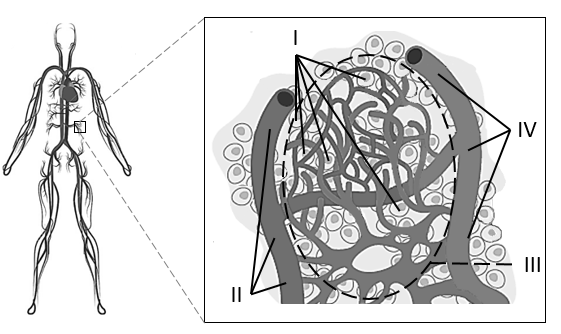
\includegraphics{img/circulatory-system.png}}
\end{center}\vspace*{-0.6cm}
\caption[Visualizaci\'on del sistema circulatorio en el organismo y de la circulaci\'on interna de un tejido]{Visualizaci\'on del sistema circulatorio en el organismo y de la circulaci\'on interna de un tejido. El sistema circulatorio es el encargado de conducir y circular la sangre por todo el organismo y la linfa unidireccionalmente hacia el coraz\'on. En la ampliaci\'on se aprecia el flujo de la circulaci\'on interna del tejido conformado por las c\'elulas~(\emph{I}) y sigue el siguiente recorrido: las arterias~(\emph{II}) traen la sangre oxigenada desde el coraz\'on, pasa por las arteriolas, capilares sangu\'ineos y v\'enulas~(\emph{III}) y finalmente desemboca en las venas~(\emph{IV}) que llevan la sangre de vuelta al coraz\'on para ser oxigenada nuevamente.}
\label{fig-circulatory}

\begin{center}
\scalebox{0.6}{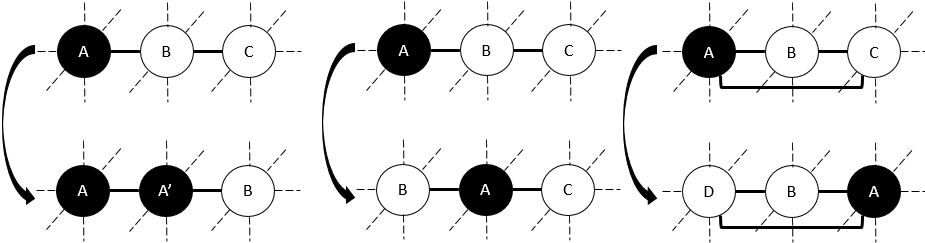
\includegraphics{img/fig-invasion.png}}
\end{center}\vspace*{-0.6cm}
\caption[Representaci\'on de las posibles interacciones entre c\'elulas cancer\'igenas y normales]{Representaci\'on de las posibles interacciones entre c\'elulas cancer\'igenas y normales.\newline
\textbf{Izquierda}: \textit{Divisi\'on Celular} - La c\'elula cancer\'igena A tiene una conexi\'on f\'isica con la c\'elula normal B. En el siguiente instante de tiempo, la c\'elula A se divide dando origen a la c\'elula cancer\'igena A' que pasa a ocupar la posici\'on de B, desplaz\'andola de la misma.\newline
\textbf{Centro}: \textit{Migraci\'on} - La c\'elula cancer\'igena A posee una mutaci\'on que le hace ganar movilidad y la posibilidad de migrar a trav\'es del tejido circundante, que le permite ocupar la posici\'on de la c\'elula normal B. En el siguiente instante de tiempo A se desplaza de su posici\'on, migra hacia B y la desplaza de su posici\'on, ocupando entonces la localizaci\'on de A.\newline
\textbf{Derecha}: \textit{Met\'astasis} - La c\'elula cancer\'igena A posee una conexi\'on distante con la c\'elula normal C, mediante su capacidad de penetrar el sistema circulatorio y abandonarlo en la posici\'on de C. En el siguiente instante de tiempo A se desplaza de su posici\'on, migra hacia C y la desplaza de su posici\'on. La localizaci\'on inicial de A es ocupada por una c\'elula normal D, descendiente de las c\'elulas vecinas de esa posici\'on.}
\label{fig-invasion}
\end{figure}

El conjunto de c\'elulas interconectadas se representa mediante una red, definida a partir de un grafo no dirigido con aristas entre vecinos inmediatos, correspondientes con el primer tipo de conexi\'on, y aristas entre v\'ertices distantes, correspondientes con el segundo tipo de conexi\'on.

\begin{definition}
\label{def-graph}
Sea $G(V, A)$ un grafo no dirigido donde los conjuntos $V$ y $A$ representan los v\'ertices y las aristas del grafo respectivamente. Se usa $V(G)$ y $A(G)$ para denotar los conjuntos de v\'ertices y aristas del grafo $G$ cuando dicho grafo no se enuncia en el contexto.
\end{definition}

\begin{definition}
\label{def-vertex-partition}
El conjunto de v\'ertices $V(G)$ est\'a dividido en dos subconjuntos $V_1(G)$ y $V_2(G)$ disjuntos que forman una partici\'on. Por tanto, satisfacen las siguientes propiedades: 
\begin{subequations}
\begin{equation}
V_1(G) \cup V_2(G) = V(G),
\end{equation}
\begin{equation}
V_1(G) \cap V_2(G) = \emptyset.
\end{equation}
\end{subequations}
\end{definition}

Los subconjuntos definidos en~\ref{def-vertex-partition} representan \'organos, tambi\'en llamadas localizaciones, que se corresponden con el \'organo primario donde se origina el c\'ancer y un \'organo preferencial de la met\'astasis, es decir, un \'organo que es colonizado con frecuencia por el tipo de c\'ancer que surgi\'o en el \'organo primario. Es necesario resaltar que ambas localizaciones pueden ser el mismo \'organo pero dos porciones distintas de tejido. Si se quiere indicar el subconjunto al que pertenece un v\'ertice $v$ determinado se utiliza la notaci\'on $V_v(G)$.

\begin{definition}
\label{def-edge-partition}
Los conjuntos $A^n(G)$ y $A^d(G)$ contienen las aristas del grafo que se corresponden con conexiones inmediatas y distantes respectivamente. Satisfacen las siguientes propiedades: 
\begin{subequations}
\begin{equation}
A^n(G) \cup A^d(G) = A(G),
\end{equation}
\begin{equation}
A^n(G) \cap A^d(G) = \emptyset.
\end{equation}
\end{subequations}
De esta manera estos subconjuntos de aristas constituyen una partici\'on del conjunto de aristas $A(G)$.
\end{definition}

A partir de los conjuntos $V(G)$ y $A(G)$ se definen los elementos representativos $\mathcal{L}$ y $\mathcal{N}$ del modelo de aut\'omatas celulares del presente trabajo de manera que se corresponda con lo expuesto en la definici\'on~\ref{def-automata}. Las declaraciones de los elementos representativos del aut\'omata celular aparecer\'an enmarcados en un recuadro negro para una mejor distinci\'on.

\begin{definition} 
\label{def-L}
El conjunto de c\'elulas $\mathcal{L}$ se define a partir del conjunto de v\'ertices del grafo $V(G)$ como se muestra a continuaci\'on: 
\begin{align}
\boxed{\mathcal{L} = V(G)}~. \label{eq-L}
\end{align}
\end{definition}

Con el objetivo de evitar ambig\"uedades y sin p\'erdida de rigor, cuando se vaya a referir al conjunto de c\'elulas siempre se utiliza el conjunto de v\'ertices $V(G)$. Los t\'erminos v\'ertice y c\'elula se utilizar\'an indistintamente. 

\begin{definition} 
\label{def-N}
La funci\'on de vecindad $\mathcal{N}$ se define a partir del conjunto de aristas del grafo $A(G)$ como se muestra a continuaci\'on:
\begin{subequations}
\begin{equation}
\boxed{\mathcal{N} : V(G) \times V(G) \rightarrow \lbrace 0,1 \rbrace}~, \label{eq-N}
\end{equation}
\begin{equation}
\boxed{\mathcal{N}(v,w) = \left\lbrace
	\begin{array}{lr}
		0& \textit{si } \lbrace v,w \rbrace \notin A(G)\\
		1& \textit{si } \lbrace v,w \rbrace \in A(G)
	\end{array}
\right.}~, \label{eq-N-2}
\end{equation}
\end{subequations}
o sea, los v\'ertices $v \in V(G)$ y $w \in V(G)$ son vecinos en el aut\'omata celular si existe una arista en $G$ que los conecta.
\end{definition}

\begin{definition}
\label{def-neighbourhood}
Se define a partir de la funci\'on de vecindad $\mathcal{N}(v,w)$ la vecindad del v\'ertice $v \in V(G)$ como el conjunto de v\'ertices $\mathcal{N}(v)$ que poseen aristas con el v\'ertice $v$, es decir:
\begin{align} 
\mathcal{N}(v) = \lbrace w~|~\mathcal{N}(v,w)=1 \rbrace. \label{eq-neighbourhood}
\end{align}
\end{definition}

\begin{definition}
\label{def-neighbourhoods}
Se define a partir del conjunto $\mathcal{N}(v)$ que contiene a los v\'ertices vecinos de $v$ los subconjuntos $\mathcal{N}^{n}(v) \subseteq \mathcal{N}(v)$ y $\mathcal{N}^{d}(v) \subseteq \mathcal{N}(v)$ que contienen los v\'ertices vecinos inmediatos y los v\'ertices vecinos distantes del v\'ertice $v$ respectivamente:
\begin{subequations}
\begin{equation}
\mathcal{N}^{n}(v) = \lbrace w~|~w \in \mathcal{N}(v) \wedge \lbrace v,w \rbrace \in A^n(G) \rbrace, \label{eq-neighbourhoods}
\end{equation}
\begin{equation}
\mathcal{N}^{d}(v) = \lbrace w~|~w \in \mathcal{N}(v) \wedge \lbrace v,w \rbrace \in A^d(G) \rbrace, \label{eq-neighbourhoods-2}
\end{equation}
\end{subequations}
\end{definition}

\section{Conjunto de c\'elulas: modelo Watts-Strogatz}
\label{subsec-watts}
En la secci\'on~\ref{subsec-vec} definimos un tejido blando como un conjunto de c\'elulas que presenta dos tipos de conexiones: entre c\'elulas vecinas cercanas y entre c\'elulas distantes. La generaci\'on de la red utilizada en el presente modelo de aut\'omatas celulares se expone a continuaci\'on. En~\cite{watts}, Duncan J. Watts y Steven H. Strogatz mostraron que existen muchas redes biol\'ogicas, tecnol\'ogicas y sociales que yacen entre las redes regulares y las aleatorias que tradicionalmente han sido utilizadas para modelar distintos tipos de sistemas din\'amicos. La clasificaci\'on y diferenciaci\'on de estas redes se lleva a cabo mediante los valores del coeficiente de agrupamiento~(\emph{clustering coefficient}) y la longitud promedio del camino~(\emph{average path length}). 

\begin{definition} 
\label{def-clustering}
Sea $v$ un v\'ertice del grafo que posee $k_v$ aristas que lo conectan a $k_v$ v\'ertices. El valor entre el n\'umero de aristas $K_v$ que existen en realidad entre estos $k_v$ v\'ertices y el n\'umero m\'aximo de aristas posibles\footnote{El n\'umero m\'aximo de aristas posibles se alcanza cuando los $k_v$ vecinos del v\'ertice $v$ pertenecen a un clique. Un clique en un grafo no dirigido es un conjunto de v\'ertices tal que para todo par de v\'ertices, existe una arista que los conecta.} $k_v(k_v-1)/2$ es el coeficiente de agrupamiento del v\'ertice $v$ y se determina como:
\begin{align}
C_v = \displaystyle\frac{2K_v}{k_v(k_v-1)}. \label{eq-clustering}
\end{align}
\end{definition}

\begin{definition}
\label{def-global-clustering}
El coeficiente de agrupamiento global del grafo $C_G$ es el promedio de todos los coeficientes de agrupamiento individuales $C_v$, es decir:
\begin{align}
C_G = \displaystyle\frac{1}{|V(G)|}\sum _{v=1} ^{|V(G)|} C_v. \label{eq-global-clustering}
\end{align}
\end{definition}

Si observamos la figura~\ref{fig-circulatory} las c\'elulas pertenecientes al tejido est\'an conectadas con numerosas c\'elulas vecinas inmediatas, y estas vecinas inmediatas est\'an conectadas entre s\'i. Dada la expresi\'on con que se determina el coeficiente de agrupamiento~(\ref{eq-clustering}) y la alta interconectividad existente se puede afirmar que la gran mayor\'ia de las c\'elulas pertenecientes al tejido poseen un alto coeficiente de agrupamiento. Por tanto, el coeficiente de agrupamiento global~(\ref{eq-global-clustering}) de la red tambi\'en posee un valor alto. 

En un grafo, la distancia entre dos v\'ertices es el menor n\'umero de aristas de un camino entre ellos. La longitud promedio del camino es la media de las distancias entre todo par de v\'ertices pertenecientes al grafo y se denota como $\ell_G$. La existencia de las numerosas conexiones distantes a trav\'es del sistema circulatorio hacen posible que el tejido posea un valor peque\~no de distancia para cualquier par de c\'elulas, ya que pueden estar conectadas mediante un camino que use estas conexiones. Podemos deducir entonces que esta red de c\'elulas posee una longitud promedio del camino relativamente peque\~na.

Como resultado podemos tomar como hip\'otesis que un tejido vivo posee un alto coeficiente de agrupamiento y una longitud promedio del camino peque\~na. Un tipo de red compleja que posee las caracter\'isticas anteriores son las redes de mundo peque\~no por lo que pueden ser utilizadas para representar un tejido vivo. Es posible generar grafos con estas caracter\'isticas usando el modelo de Watts y Strogatz~\cite{watts}. Los autores proponen un modelo de un solo par\'ametro que devuelve una red de mundo peque\~no, ubicada entre un grafo regular y un grafo aleatorio. El algoritmo propuesto por el modelo, que es utilizado para generar las redes de mundo peque\~no usadas en el presente trabajo, es el siguiente~\cite{complexnetworks}:

\begin{enumerate}
\item [(1)] \emph{Inicio:} Comenzamos con un grafo con $q$ v\'ertices, e.g. un anillo o una malla, en los que cada v\'ertice est\'a conectado a $k$ vecinos inmediatos. 

\item [(2)] \emph{Aleatorizaci\'on:} Reconectamos de forma aleatoria cada arista del grafo con una probabilidad $p$ de tal forma que no existan aristas duplicadas ni bucles. Este procedimiento introduce $\frac{p\,*\,q\,*\,k}{2} $ aristas que conectan v\'ertices distantes. Mediante la variaci\'on de $p$, se puede observar la transici\'on entre el orden con $p = 0$ y un grafo totalmente aleatorio con $p = 1$~(Fig.~\ref{fig-relations}).
\end{enumerate}

\begin{figure}[!ht]
\begin{center}
\scalebox{0.6}{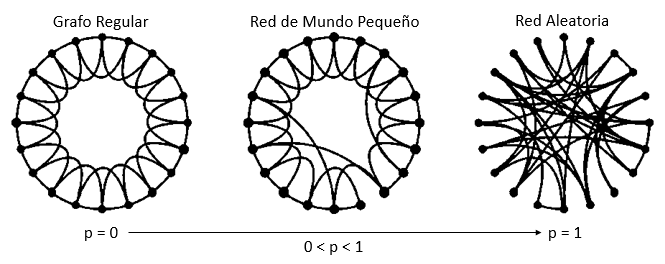
\includegraphics{img/fig-relations.png}}
\end{center}\vspace*{-0.6cm}
\caption[Proceso de reconexi\'on aleatoria del modelo Wattz-Strogatz]{Proceso de reconexi\'on aleatoria del modelo Wattz-Strogatz~(Figura tomada de~\cite{complexnetworks}). Se fijan $q = 20$ v\'ertices, cada uno conectado a sus cuatro vecinos m\'as cercanos. Para $p = 0$ el anillo original se queda inalterado, y a medida que se incrementa $p$ la red se vuelve desordenada. Para $p = 1$ todas las aristas del grafo son reconectadas.}
\label{fig-relations}
\end{figure}

\subsection{Implementaci\'on del modelo Watts-Strogatz}
\label{subsec-watts-2}
El modelo Watts-Strogatz, tomando en cuenta la hip\'otesis XII sobre la representaci\'on del tejido, parte de un grafo en el que cada v\'ertice ha sido conectado con un n\'umero de sus vecinos inmediatos. Las aristas que conforman el grafo son sometidas a un proceso de reconexi\'on, donde se modifica uno de los extremos de la arista. El nuevo extremo se elige de entre los v\'ertices restantes del grafo de forma aleatoria. Para el proceso de construcci\'on consideremos una cuadr\'icula que divide el plano en secciones iguales, donde cada celda se corresponde con un v\'ertice del grafo~(Fig.~\ref{fig-grid-2D-initial}).

\begin{figure}[!ht]
\begin{center}
\scalebox{0.7}{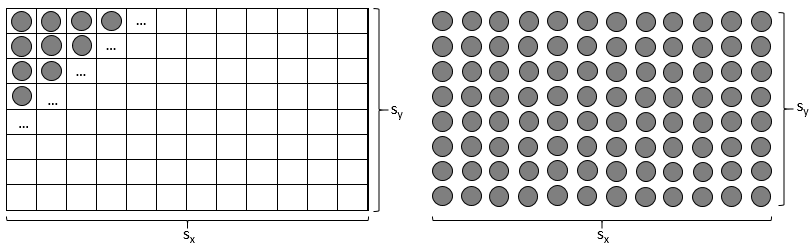
\includegraphics{img/fig-grid-2D-initial.png}}
\end{center}\vspace*{-0.6cm}
\caption[Disposici\'on espacial de los v\'ertices del grafo]{Disposici\'on espacial de los v\'ertices del grafo determinados mediante la cuadr\'icula que se muestra en la imagen izquierda, y que divide el plano en partes iguales para un total de $q = s_x \times s_y = 12 \times 8 = 96$ v\'ertices como se muestra en la imagen derecha.}
\label{fig-grid-2D-initial}
\end{figure}

Como se expuso en la definici\'on~\ref{def-neighbourhoods} el presente modelo de aut\'omatas celulares hace uso de los conjuntos $A^n(G)$ y $A^d(G)$ de aristas del grafo que se corresponden con conexiones inmediatas y distantes respectivamente. La idea de la implementaci\'on del modelo Watts-Strogatz para la construcci\'on del grafo es agregar todas las aristas inmediatas al conjunto $A^n(G)$ y a medida que sean reconectadas son removidas de este conjunto y se a\~naden a $A^d(G)$. Existen varias alternativas a la hora de elegir las conexiones inmediatas de cada v\'ertice donde cada una tiene un impacto importante sobre las propiedades de la red. En la figura~\ref{fig-neighbour} se pueden apreciar algunos diagramas de posibles configuraciones de vecindad. Comenzamos exponiendo la definici\'on de la distancia euclideana para definir posteriormente una funci\'on que permite obtener la vecindad inmediata de un v\'ertice. 

\begin{definition}
\label{def-euclidean-distance}
La funci\'on $d_E(v,w)$, que recibe dos v\'ertices $v \in V(G)$ y $w \in V(G)$, se corresponde con la distancia euclidiana entre los dos puntos del espacio que ocupan dichos v\'ertices y se determina como:
\begin{equation}
d_E(v,w)=\sqrt{(v_x-w_x)^2 + (v_y-w_y)^2}.
\end{equation}
\end{definition}

\begin{definition}
\label{def-neighbourhood-template}
Dado un v\'ertice $v$ en el sistema de coordenadas cartesianas que se utiliz\'o para crear la malla original, definimos como vecindad inmediata de $v$ al conjunto de v\'ertices $\mathcal{N}_I(v,R) = \lbrace w_1, w_2, \ldots, w_m \rbrace$ con $m=|\mathcal{N}_I(v,R)|$ que cumplen la condici\'on $d_E(v,w) \leq R$, es decir:
\begin{equation}
\mathcal{N}_I(v,R) = \lbrace w | d_E(v,w) \leq R \rbrace.
\end{equation}
\end{definition} 

\begin{figure}[!ht]
\begin{center}
\scalebox{0.5}{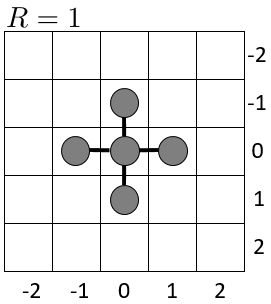
\includegraphics{img/fig-neighbour-R-1.png}}
\scalebox{0.5}{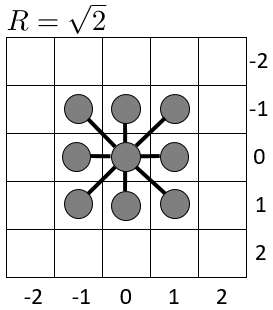
\includegraphics{img/fig-neighbour-R-sqrt(2).png}}
\scalebox{0.5}{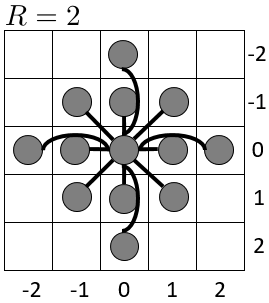
\includegraphics{img/fig-neighbour-R-2.png}}
\scalebox{0.5}{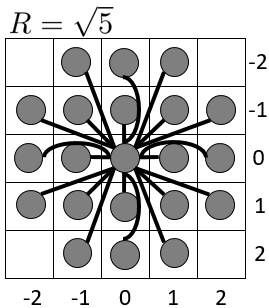
\includegraphics{img/fig-neighbour-R-sqrt(5).png}}
\end{center}\vspace*{-0.6cm}
\caption[Configuraciones de vecindad obtenidas mediante la variaci\'on de $R$]{Configuraciones de vecindad obtenidas mediante la variaci\'on de $R$. En todos los diagramas el v\'ertice $v=(0,0)$ es el centro de la configuraci\'on y se muestra en cada uno el valor de $R$ utilizado para generarla.}
\label{fig-neighbour}
\end{figure}

Es necesario tambi\'en discutir la inclusi\'on de aristas peri\'odicas al grafo. Una arista peri\'odica conecta dos extremos opuestos de la malla, por lo que la inclusi\'on de estas aristas constituye la implementaci\'on de una frontera peri\'odica en la malla. El modelo Watts-Strogatz asegura que el grafo creado posee las propiedades expuestas si todos los v\'ertices tienen el mismo grado, pero como se puede apreciar, un v\'ertice perteneciente a uno o varios lados del plano definido ser\'a referenciado por un n\'umero menor de aristas. La necesidad de incluir aristas peri\'odicas es una forma de hacer que estos v\'ertices posean el grado adecuado. La desventaja de este procedimiento es la ausencia de una interpretaci\'on natural de dichas aristas peri\'odicas por el modelo de aut\'omatas celulares que se presenta en este manuscrito. Se infiere que la inclusi\'on de estas aristas al grafo posee influencia sobre las propiedades del mismo. 

La selecci\'on de un valor adecuado de $R$, la probabilidad de reconexi\'on $p$ y la inclusi\'on de aristas peri\'odicas son los factores que determinan las propiedades del grafo resultante, cuestiones que se abordan en la secci\'on~\ref{subsec-R-periodic}. Finalmente, la implementaci\'on del modelo Watts-Strogatz se expone en el algoritmo~\ref{alg-watts} y los procedimientos que se llevan a cabo se detallan a continuaci\'on para mayor claridad.

\begin{algorithm}[!ht]
\caption{Implementaci\'on del Modelo Watts-Strogatz.} \label{alg-watts}
\KwData{$s_x, s_y, s_o, p, R$}
\KwResult{$G$}
$V_1=\lbrace \rbrace$\;
$V_2=\lbrace \rbrace$\;
$A^n=\lbrace \rbrace$\;
$A^d=\lbrace \rbrace$\;
\For{$i=0,1,\ldots,s_x-1$}{
	\For{$j=0,1,\ldots,s_y-1$}{
		$v=(i,j)$\;
		\eIf{$i < s_o$}{
			$V_1 = V_1 \cup v $\;}{
			$V_2 = V_2 \cup v $\;}}}
$V=V_1 \cup V_2$\;
\For{$v \in V$}{
	\For{$w \in N_I(v,R)$}{
		$a=\lbrace v,w \rbrace$\;
		$A^n=A^n \cup \lbrace a \rbrace$\;}}
\For{$\lbrace v,w \rbrace \in A^n$}{
	\If{$Random(0,1)<p$}{
		$A^n = A^n \setminus \lbrace v,w \rbrace$\;
		\Repeat{$\lbrace v,w' \rbrace \notin A^n \wedge \lbrace v,w' \rbrace \notin A^d \wedge v \neq w'$}
			{$w'=Select$-$Random$-$Vertex(V)$\;}
		$A^d = A^d \cup \lbrace v,w' \rbrace$\;}}
$A=A^n \cup A^d$\;
$G=(V,A)$\;
\Return $G$\;
\end{algorithm}

\paragraph{Declaraci\'on de los conjuntos que componen el grafo $G$ ($1$-$4$):} Se declaran los conjuntos $V_1$, $V_2$, $A_n$ y $A_d$, inicialmente vac\'ios, correspondientes con los v\'ertices de las localizaciones primaria y secundaria, y las conexiones inmediatas y distantes respectivamente. 

\paragraph{Crear v\'ertices ($5$-$11$):} Se a\~naden a los conjuntos $V_1$ y $V_2$ los v\'ertices que conforman el grafo. Cada v\'ertice $v$ de coordenadas $(v_x,v_y)$ se corresponde con una celda de la malla. Los valores $s_x$ y $s_y$ son las cantidades de v\'ertices del grafo por cada una de las componentes del plano respectivamente~(Fig.~\ref{fig-grid-2D-initial}). Cada v\'ertice se a\~nade al conjunto $V_1$ o $V_2$ correspondiente, que se determina a partir del par\'ametro $s_o$ con $0 \leq s_o < s_x$ que indica la divisi\'on del grafo entre una localizaci\'on y la otra. 

\paragraph{A\~nadir aristas inmediatas ($12$-$16$):} Se itera por todos los v\'ertices del grafo resultado de la uni\'on de los conjuntos $V_1$ y $V_2$. Por cada v\'ertice $v \in V$ se obtiene su vecindad inmediata $N_I(v,R)$ y se itera por todos los v\'ertices vecinos. Se crea una arista entre $v$ y cada v\'ertice vecino $w$ y se a\~nade al conjunto de aristas inmediatas $A^n$. Dado que la uni\'on entre conjuntos da como resultado un conjunto donde no existen elementos repetidos, no es necesario verificar si una nueva arista ya pertenece al conjunto $A^n$ antes de ser a\~nadida.

\paragraph{Reconexi\'on de las aristas ($17$-$26$):} Se itera por cada arista $a$ del grafo y con probabilidad $p$ se reconecta el v\'ertice destino de la arista. La generaci\'on del valor aleatorio que se compara con $p$ para el c\'alculo de la probabilidad sigue una distribuci\'on uniforme en $(0,1)$. La arista $\lbrace v,w \rbrace$ seleccionada para su reconexi\'on se elimina del conjunto $A^n$ y se procede a encontrar el nuevo v\'ertice destino. El nuevo v\'ertice destino $w'$ se elige de entre todos los v\'ertices del grafo, pero no puede ser el origen de la arista porque no se permiten bucles, y la nueva arista formada no puede existir en el grafo ya que no se permiten duplicados. La nueva arista $\lbrace v,w' \rbrace$ se a\~nade al conjunto $A^d$, identificando satisfactoriamente la nueva conexi\'on como distante. Finalmente, se realiza la uni\'on de los conjuntos $A^n$ y $A^d$, y se declara el grafo $G$ que se retorna como resultado del algoritmo. En la figura~\ref{fig-grid-2D-reconected} se puede apreciar la disposici\'on de los v\'ertices de las caras externas y las conexiones distantes una vez concluido el procedimiento.

\begin{figure}[!ht]
\begin{center}
\scalebox{0.65}{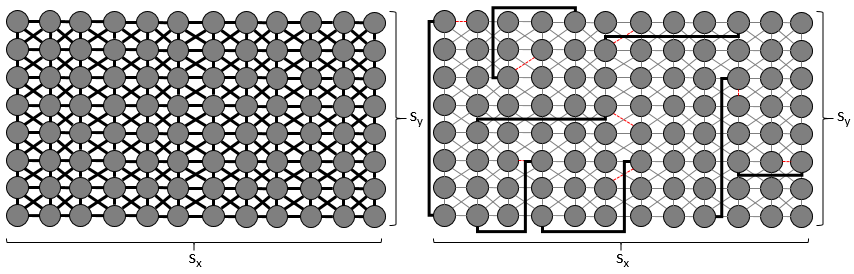
\includegraphics{img/fig-grid-2D-reconected.png}}
\end{center}\vspace*{-0.6cm}
\caption[Detalles de la disposici\'on de las aristas inmediatas y reconectadas en el grafo]{Detalles de la disposici\'on de las aristas inmediatas y reconectadas en el grafo presentado en la figura~\ref{fig-grid-2D-initial}. En el diagrama izquierdo se muestra el grafo construido utilizando la configuraci\'on de vecindad generada con $R=2$, y en el derecho se muestra el grafo una vez concluido el proceso de reconexi\'on de las aristas.}
\label{fig-grid-2D-reconected}
\end{figure}

\subsection{Propiedades del grafo resultante del modelo Watts-Strogatz}
\label{subsec-R-periodic}
En la secci\'on anterior se expuso que el valor del radio de la vecindad inmediata $R$ y las aristas peri\'odicas determinan las propiedades del grafo generado mediante el modelo Watts-Strogatz. Se propone en esta secci\'on exponer estad\'isticamente la medida en que afecta el coeficiente de agrupamiento global de la red y la longitud promedio del camino la ausencia o presencia de estas aristas en conjunci\'on con varios valores de $R$. Con el objetivo de efectuar esta prueba el algoritmo~\ref{alg-watts} puede alternar entre la inclusi\'on o no de las aristas peri\'odicas. Si se toma que la distancia euclideana entre dos v\'ertices que se encuentran en extremos opuestos del grafo $v$ y $w$ es igual a $1$~(siendo $R=1$ el menor valor de radio de la vecindad concebido) entonces la arista peri\'odica entre $v$ y $w$ estar\'a contenida en las vecindades inmediatas de estos v\'ertices. La implementaci\'on de esta condici\'on permite alternar entre la inclusi\'on o no de aristas peri\'odicas al grafo resultante.

Para verificar el impacto de las distintas configuraciones de vecindad inmediatas y de la inclusi\'on o no de aristas peri\'odicas en los valores del coeficiente de agrupamiento $C_G$ y de la longitud promedio del camino de la red $\ell_G$ se realizaron diversas pruebas mediante la construcci\'on de distintas redes con una cantidad total de $q = s_x \times s_y = 40 \times 20 = 800$ v\'ertices y alternando distintos valores de $R$ y $p$ con la inclusi\'on o no de aristas peri\'odicas. Cada uno de los valores de $C_G$ y $\ell_G$, mostrados en el cuadro~\ref{table-network-data}, fueron obtenidos promediando los resultados provenientes de la realizaci\'on de $30$ ejecuciones. 
\begin{table}[!ht]
\begin{center}
\scalebox{0.9}{\begin{tabular}{|c|c|c|c|c|c|c|c|c|} \hline
\multicolumn{3}{|c|}{\emph{Par\'ametros}} & \multicolumn{6}{|c|}{\emph{Probabilidad de reconexi\'on}} \\\cline{4-9}

\multicolumn{3}{|c|}{} & \multicolumn{1}{|l|}{$p=0~~$} & \multicolumn{1}{|l|}{$p=10^{-4}$} & \multicolumn{1}{|l|}{$p=10^{-3}$} & \multicolumn{1}{|l|}{$p=10^{-2}$} & \multicolumn{1}{|l|}{$p=10^{-1}$} & \multicolumn{1}{|l|}{$p=1~~$} \\\hline

 & \emph{Aristas} & $C_G$ & \multicolumn{1}{|r|}{$0$} & \multicolumn{1}{|r|}{$0$} & \multicolumn{1}{|r|}{$0$.$0001$} & \multicolumn{1}{|r|}{$0$.$0001$} & \multicolumn{1}{|r|}{$0$.$0007$} & \multicolumn{1}{|r|}{$0$.$0007$} \\\cline{3-9}
 
$R=1$ & \emph{peri\'odicas} & $\ell_G$ & \multicolumn{1}{|r|}{$15$} & \multicolumn{1}{|r|}{$14$.$9699$} & \multicolumn{1}{|r|}{$14$.$1113$} & \multicolumn{1}{|r|}{$10$.$2807$} & \multicolumn{1}{|r|}{$6$.$6847$} & \multicolumn{1}{|r|}{$5$.$1387$} \\\cline{2-9}

 & \emph{No aristas} & $C_G$ & \multicolumn{1}{|r|}{$0$} & \multicolumn{1}{|r|}{$0$} & \multicolumn{1}{|r|}{$0$} & \multicolumn{1}{|r|}{$0$} & \multicolumn{1}{|r|}{$0$.$0007$} & \multicolumn{1}{|r|}{$0$.$0042$} \\\cline{3-9}
 
 & \emph{peri\'odicas} & $\ell_G$ & \multicolumn{1}{|r|}{$19$.$975$} & \multicolumn{1}{|r|}{$19$.$8841$} & \multicolumn{1}{|r|}{$17$.$0731$} & \multicolumn{1}{|r|}{$11$.$8948$} & \multicolumn{1}{|r|}{$7$.$0317$} & \multicolumn{1}{|r|}{$5$.$2847$} \\\hline

 & \emph{Aristas} & $C_G$ & \multicolumn{1}{|r|}{$0$.$4284$} & \multicolumn{1}{|r|}{$0$.$4283$} & \multicolumn{1}{|r|}{$0$.$4271$} & \multicolumn{1}{|r|}{$0$.$4151$} & \multicolumn{1}{|r|}{$0$.$3155$} & \multicolumn{1}{|r|}{$0$.$0088$} \\\cline{3-9}
 
$R=\sqrt{2}$ & \emph{peri\'odicas} & $\ell_G$ & \multicolumn{1}{|r|}{$10$.$8165$} & \multicolumn{1}{|r|}{$10$.$6258$} & \multicolumn{1}{|r|}{$9$.$2563$} & \multicolumn{1}{|r|}{$6$.$6914$} & \multicolumn{1}{|r|}{$4$.$4453$} & \multicolumn{1}{|r|}{$3$.$4615$} \\\cline{2-9}

 & \emph{No aristas} & $C_G$ & \multicolumn{1}{|r|}{$0$.$4554$} & \multicolumn{1}{|r|}{$0$.$4554$} & \multicolumn{1}{|r|}{$0$.$4538$} & \multicolumn{1}{|r|}{$0$.$4423$} & \multicolumn{1}{|r|}{$0$.$3334$} & \multicolumn{1}{|r|}{$0$.$0089$} \\\cline{3-9}

 & \emph{peri\'odicas} & $\ell_G$ & \multicolumn{1}{|r|}{$14$.$8229$} & \multicolumn{1}{|r|}{$14$.$664$} & \multicolumn{1}{|r|}{$11$.$3451$} & \multicolumn{1}{|r|}{$7$.$5682$} & \multicolumn{1}{|r|}{$4$.$6398$} & \multicolumn{1}{|r|}{$3$.$5439$} \\\hline
    
 & \emph{Aristas} & $C_G$ & \multicolumn{1}{|r|}{$0$.$4328$} & \multicolumn{1}{|r|}{$0$.$4326$} & \multicolumn{1}{|r|}{$0$.$4228$} & \multicolumn{1}{|r|}{$0$.$4209$} & \multicolumn{1}{|r|}{$0$.$3219$} & \multicolumn{1}{|r|}{$0$.$0137$} \\\cline{3-9}
 
$R=2$ & \emph{peri\'odicas} & $\ell_G$ & \multicolumn{1}{|r|}{$7$.$6976$} & \multicolumn{1}{|r|}{$7$.$4887$} & \multicolumn{1}{|r|}{$6$.$9479$} & \multicolumn{1}{|r|}{$5$.$1801$} & \multicolumn{1}{|r|}{$3$.$6611$} & \multicolumn{1}{|r|}{$2$.$9432$} \\\cline{2-9}

 & \emph{No aristas} & $C_G$ & \multicolumn{1}{|r|}{$0$.$4731$} & \multicolumn{1}{|r|}{$0$.$4729$} & \multicolumn{1}{|r|}{$0$.$4716$} & \multicolumn{1}{|r|}{$0$.$4595$} & \multicolumn{1}{|r|}{$0$.$3506$} & \multicolumn{1}{|r|}{$0$.$0126$} \\\cline{3-9}
 
 & \emph{peri\'odicas} & $\ell_G$ & \multicolumn{1}{|r|}{$10$.$2375$} & \multicolumn{1}{|r|}{$9$.$8962$} & \multicolumn{1}{|r|}{$8$.$5608$} & \multicolumn{1}{|r|}{$5$.$6387$} & \multicolumn{1}{|r|}{$3$.$8089$} & \multicolumn{1}{|r|}{$3$.$0155$} \\\hline

 & \emph{Aristas} & $C_G$ & \multicolumn{1}{|r|}{$0$.$5157$} & \multicolumn{1}{|r|}{$0$.$5155$} & \multicolumn{1}{|r|}{$0$.$5138$} & \multicolumn{1}{|r|}{$0$.$501$} & \multicolumn{1}{|r|}{$0$.$3832$} & \multicolumn{1}{|r|}{$0$.$0235$} \\\cline{3-9}
 
$R=\sqrt{5}$ & \emph{peri\'odicas} & $\ell_G$ & \multicolumn{1}{|r|}{$5$.$9356$} & \multicolumn{1}{|r|}{$5$.$7967$} & \multicolumn{1}{|r|}{$5$.$0588$} & \multicolumn{1}{|r|}{$3$.$9797$} & \multicolumn{1}{|r|}{$3$.$0175$} & \multicolumn{1}{|r|}{$2$.$5704$} \\\cline{2-9}

 & \emph{No aristas} & $C_G$ & \multicolumn{1}{|r|}{$0$.$5697$} & \multicolumn{1}{|r|}{$0$.$5696$} & \multicolumn{1}{|r|}{$0$.$5679$} & \multicolumn{1}{|r|}{$0$.$5526$} & \multicolumn{1}{|r|}{$0$.$4186$} & \multicolumn{1}{|r|}{$0$.$0217$} \\\cline{3-9}

 & \emph{peri\'odicas} & $\ell_G$ & \multicolumn{1}{|r|}{$7$.$9587$} & \multicolumn{1}{|r|}{$7$.$6352$} & \multicolumn{1}{|r|}{$6$.$1198$} & \multicolumn{1}{|r|}{$4$.$2943$} & \multicolumn{1}{|r|}{$3$.$1359$} & \multicolumn{1}{|r|}{$2$.$6226$} \\\hline
\end{tabular}}
\end{center}\vspace*{-0.6cm}
\caption[Datos de las pruebas realizadas para verificar el impacto de las distintas configuraciones de vecindad y de la inclusi\'on de aristas peri\'odicas en las propiedades del grafo]{Datos de las pruebas realizadas para verificar el impacto de las distintas configuraciones de vecindad y de la inclusi\'on de aristas peri\'odicas en los valores del coeficiente de agrupamiento $C_G$ y de la longitud promedio del camino de la red $\ell_G$. }
\label{table-network-data}
\end{table}

Se observa que para un mismo valor de $R$ e independientemente si se incluyen o no las aristas peri\'odicas, a medida que aumenta el valor de la probabilidad de reconexi\'on $p$ disminuye el coeficiente de agrupamiento global y disminuye la longitud promedio del camino, observ\'andose la mayor disminuci\'on a medida que $p$ se acerca a $1$. Esto ocurre porque a medida que m\'as aristas inmediatas son reconectadas a v\'ertices distantes es menor la probabilidad de que estos v\'ertices distantes est\'en conectados con los vecinos inmediatos del v\'ertice focal, disminuyendo el valor del coeficiente de agrupamiento del grafo; pero a medida que aparecen m\'as aristas distantes aumenta la probabilidad de que dos v\'ertices aleatorios est\'en conectados a trav\'es de un camino m\'as corto que utilice estas aristas, disminuyendo la longitud promedio del camino.

Adem\'as se cumple para toda combinaci\'on de $R$ y $p$ que la ausencia de aristas peri\'odicas en el grafo hace que la longitud promedio del camino aumente, dado que permiten la existencia de posibles caminos entre v\'ertices distantes que poseen distancias menores que los caminos que no cuentan con dichas aristas. Pero la ausencia de aristas peri\'odicas, salvo para $p=1$, provoca tambi\'en un aumento en el coeficiente de agrupamiento del grafo, dado que los v\'ertices que poseen vecinos conectados por aristas peri\'odicas aportan valores peque\~nos del coeficiente de agrupamiento ya que existen muchos casos donde dichos v\'ertices vecinos no est\'an conectados entre s\'i.

Dado que la presencia de aristas peri\'odicas carece de una interpretaci\'on natural como se mencion\'o en la secci\'on~\ref{subsec-watts-2}, y que no afectan de forma negativa las propiedades deseadas del grafo resultante como se expuso en el texto anterior, se decide no incluirlas. Se elige la configuraci\'on de vecindad generada con $R=\sqrt{2}$ ya que los grafos construidos con este valor poseen coeficientes de agrupamiento altos y longitudes promedio del camino relativamente peque\~nas. Adem\'as constituye la configuraci\'on de vecindad m\'as sencilla que posee las caracter\'isticas mencionadas ya que provee de una interpretaci\'on natural para las conexiones inmediatas correspondientes con la cercan\'ia f\'isica a diferencia de otras vecindades generadas con valores mayores de $R$; e.g. para $R=2$ se tienen v\'ertices vecinos a distancia $2$ del v\'ertice central. En cuanto a la probabilidad de reconexi\'on esta se encuentra entre los valores $p \in \lbrace 10^{-3}, 10^{-2} \rbrace$ en los que ocurre un r\'apido descenso en el valor de la longitud promedio del camino mientras que el coeficiente de agrupamiento se mantiene casi invariante con un valor cercano a $C_G=0$.$45$ para $R=\sqrt{2}$, que si atendemos lo planteado en~\cite{complexnetworks} constituye un valor alto.

\section{Conjunto de estados}
\label{subsec-states}
Un estado en teor\'ia de aut\'omatas celulares es un valor num\'erico que se le asigna inicialmente a cada elemento del conjunto de c\'elulas y puede cambiar en el transcurso de la ejecuci\'on. En este modelo el estado indica el tipo de c\'elula biol\'ogica en la que estamos en presencia. Un corte transversal del tejido revela que est\'a estructurado en capas donde cada una posee una funci\'on espec\'ifica dentro del \'organo~(Fig.~\ref{fig-structure}). El desarrollo macrosc\'opico de un tumor depende en gran medida de las interacciones progresivas entre la masa de las c\'elulas cancer\'igenas y cada una de estas capas de tejidos. En \'epocas pasadas de la histolog\'ia\footnote{La histolog\'ia es la disciplina que estudia todo lo relacionado con los tejidos org\'anicos: su estructura microsc\'opica, su desarrollo y sus funciones.} se clasificaba cada capa del tejido como parte del par\'enquima o del estroma. Se reconoce como par\'enquima al tejido que desempe\~na la funci\'on principal de un \'organo espec\'ifico, mientras que las capas de tejido que hacen de sost\'en y apoyo al tejido funcional se llama estroma. Generalmente el par\'enquima est\'a conformado por el epitelio de un \'organo. En la secci\'on~\ref{subsec-macro} se expuso el desarrollo idealizado de un tumor que se origina en c\'elulas de tipo epitelial o carcinoma, y su expansi\'on a trav\'es de las distintas capas de tejidos. Por lo que, en primera instancia, se requiere de un estado para las c\'elulas del tejido epitelial.

\begin{figure}[!ht]
\begin{center}
\scalebox{0.6}{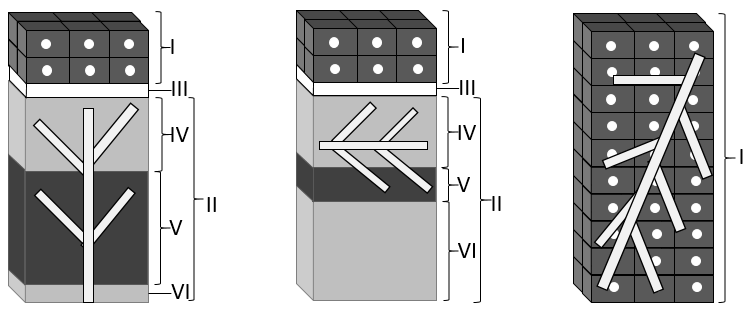
\includegraphics{img/fig-structure.png}}
\end{center}\vspace*{-0.6cm}
\caption[Distribuci\'on de las capas de tejidos en distintos \'organos]{Distribuci\'on de las capas de tejidos en distintos \'organos afectados com\'unmente por el tipo de c\'ancer conocido como carcinoma~\cite{robins}.\newline
\textbf{Izquierda}: \textit{Aparato digestivo} - La estructura mostrada est\'a presente en el es\'ofago, est\'omago, intestinos y recto~\cite{stomach}. Como se puede apreciar todos los tejidos de sost\'en presentan vasculatura. Todas las formas de carcinomas que afectan al aparato digestivo comienzan en la mucosa: carcinoma de c\'elulas escamosas del es\'ofago, adenocarcinoma g\'astrico y adenocarinoma colonrectal. La leyenda se muestra a continuaci\'on: mucosa~(\emph{I}) - formada por epitelio escamoso estratificado en el es\'ofago y por epitelio cil\'indrico columnar en est\'omago e intestinos; estroma~(\emph{II}) - tejidos de sost\'en; membrana basal~(\emph{III}); submucosa~(\emph{IV}) - formada por tejido conjuntivo; muscularis propia~(\emph{V}); serosa~(\emph{VI}).\newline
\textbf{Centro}: \textit{Pulm\'on} - La estructura mostrada est\'a presente en las v\'ias a\'ereas inferiores compuestas por tr\'aquea, bronquios y bronquiolos~\cite{lung}. Como se puede apreciar todos los tejidos de sost\'en con la excepci\'on del cart\'ilago hialino presentan vasculatura. El carcinoma pulmonar de c\'elulas escamosas comienza en la mucosa de los bronquios en la mayor\'ia de los casos. La leyenda se muestra a continuaci\'on: mucosa~(\emph{I}) - formada por epitelio pseudoestratificado columnar en la tr\'aquea y bronquios primarios y por epitelio simple cil\'indrico en los bronquiolos; estroma~(\emph{II}) - tejidos de sost\'en; membrana basal~(\emph{III}); submucosa~(\emph{IV}) - formada por tejido conjuntivo; m\'usculo liso~(\emph{V}); cart\'ilago hialino~(\emph{VI}) - formado por tejido conjuntivo duro.\newline
\textbf{Derecha}: \textit{H\'igado} - El h\'igado est\'a conformado por su propio tipo de c\'elula: los hepatocitos~(\emph{I}) y constituyen su par\'enquima~\cite{liver}. Los vasos del sistema circulatorio est\'an presentes a lo largo del \'organo. El c\'ancer de h\'igado que surge en esta clase de c\'elulas se considera como un carcinoma y se conoce como hepatocarcinoma, aunque las met\'astasis en el h\'igado de otros tipos de c\'ancer son mucho m\'as frecuentes que los que comienzan en el propio \'organo.}
\label{fig-structure}
\end{figure}

Se han hecho progresos en el entendimiento de las complejas interacciones entre el tumor y el tejido sano del organismo, en especial las responsables de los comportamientos invasivos y migratorios del c\'ancer, pero muchos mecanismos no son comprendidos en su totalidad o se desconocen por completo en este momento~\cite{kansal3}. Sin embargo se pueden distinguir varios procesos responsables de la invasi\'on y migraci\'on: la degradaci\'on de la membrana basal que se desarrolla durante la angiog\'enesis, la deformaci\'on y desplazamiento del estroma como consecuencia de las fuerzas generadas por la expansi\'on del tumor y la degradaci\'on de la ECM~\cite{kansal3}. El tipo de c\'elula cancer\'igena que entra en contacto con el estroma define cual proceso se llevar\'a a cabo. La invasi\'on se lleva a cabo por c\'elulas cancer\'igenas pertenecientes a la masa del tumor una vez que se ha degradado la membrana basal, y la migraci\'on por c\'elulas cancer\'igenas que poseen las mutaciones para desplazarse a trav\'es del estroma mediante la degradaci\'on de la ECM. 

A pesar de la heterogeneidad de los tejidos que conforman el estroma, las interacciones entre la totalidad de los tejidos de sost\'en y las c\'elulas cancer\'igenas resultan en uno de estos dos procesos: invasi\'on o migraci\'on. Por este motivo no es necesario distinguir entre las distintas capas de tejidos de sost\'en en el aut\'omata celular si solo se tienen en cuenta estas interacciones fundamentales. Luego se adopta una nueva hip\'otesis en el modelo que reduce la complejidad de la din\'amica del aut\'omata celular, representando los distintos tipos de tejidos de sost\'en simplemente como estroma. Las c\'elulas del aut\'omata correspondientes a este tejido se corresponden entonces a c\'elulas biol\'ogicas reales o a cl\'usteres de macromol\'eculas presentes en la ECM. 

\begin{itemize}
\item [{XIII.}] \textbf{Tejidos de sost\'en o estroma}: \emph{Se representa a la totalidad de los tejidos de sost\'en de un \'organo simplemente como estroma debido a que solo se consideran dos interacciones fundamentales entre los tejidos sanos y el c\'ancer: la invasi\'on y la migraci\'on. Por este motivo no es necesario hacer distinciones entre las distintas capas de sost\'en.} \label{XIII}
\end{itemize}

El tejido epitelial recubre toda superficie del cuerpo humano que tiene contacto con el exterior, e.g. \'organos huecos, como el est\'omago y pulmones, o estructuras tubulares, como los bronquios y arterias. Estos espacios se conocen como luz de un \'organo o lumen, en el caso de los bronquios, arterias e intestinos. En los carcinomas es com\'un que la masa tumoral brote fuera del epitelio, evadiendo los controles de homeostasis del tejido y volvi\'endose una lesi\'on. La manifestaci\'on fuera del epitelio constituye un marcador visible del desarrollo neopl\'asico, por lo que la luz de un \'organo o lumen debe ser representada~\cite{robins,stomach,lung,liver,breast}. A partir de lo expuesto anteriormente se infieren los estados para las c\'elulas normales. A continuaci\'on se define formalmente el estado de una c\'elula del aut\'omata:

\begin{definition}
\label{def-cellstatus}
Sea un v\'ertice $v \in V(G)$ y un instante de tiempo $n$ del aut\'omata. Se define entonces la funci\'on $s(v,n)$ que devuelve el estado del v\'ertice $v$ en el instante de tiempo $n$:
\begin{subequations}
\begin{equation}
s: V(G) \times \mathbb{N} \rightarrow \mathcal{E}, \label{eq-cellstatus}
\end{equation}
\begin{equation}
s(v,n) = e_i, \label{eq-cellstatus-2}
\end{equation}
\end{subequations}
donde $e_i$ es un estado cualquiera del conjunto de estados $\mathcal{E}$, es decir, $e_i \in \mathcal{E},~\forall i \in \lbrace 0, \ldots, |\mathcal{E}| \rbrace$.
\end{definition}

A continuaci\'on, tomando en cuenta la hip\'otesis XIII sobre los tejidos de sost\'en, se disponen los estados para las c\'elulas normales del aut\'omata:

\begin{itemize}
\item $s(v,n)=0$: El v\'ertice $v$ posee el estado correspondiente con el espacio vac\'io o lumen en el instante de tiempo $n$, y representa las cavidades huecas de los \'organos y conductos.

\item $s(v,n)=1$: El v\'ertice $v$ representa una c\'elula del epitelio en el instante de tiempo $n$, y corresponde con el tejido donde se origina el carcinoma.

\item $s(v,n)=2$: El v\'ertice $v$ posee el estado correspondiente con el estroma en el instante de tiempo $n$, y representa el conjunto de tejidos de sost\'en del \'organo.
\end{itemize}

En cuanto a las c\'elulas cancer\'igenas se distinguen tres estados fundamentales basado en las hip\'otesis del modelo y en lo expuesto en la secci\'on~\ref{sec-cancer}:

\begin{itemize}
\item $s(v,n)=3$: El v\'ertice $v$ representa una c\'elula tumoral en el instante de tiempo $n$, y constituyen la masa neopl\'asica.

\item $s(v,n)=4$: El v\'ertice $v$ representa una c\'elula migratoria en el instante de tiempo $n$, es decir, poseen las mutaciones necesarias para efectuar la cascada metast\'asica.

\item $s(v,n)=5$: El v\'ertice $v$ representa una c\'elula micrometast\'asica en el instante de tiempo $n$, es decir, efectuaron la cascada metast\'a\-sica satisfactoriamente y est\'an colonizando la nueva localizaci\'on, pero pueden ser destruidas por el sistema inmunitario o fallar en dicha colonizaci\'on. 
\end{itemize}

Luego el conjunto de estados tiene la forma:
\begin{equation}
\boxed{\mathcal{E} = \lbrace 0, 1, 2, 3, 4, 5 \rbrace}~. \label{eq-states}
\end{equation}

Inicialmente se asigna a cada c\'elula el estado correspondiente a partir de su posici\'on en el tejido de cada localizaci\'on representada en el aut\'omata, es decir, se reproduce la estructura de los tejidos expuestos en la figura~\ref{fig-structure} a partir de la asignaci\'on correspondiente de los distintos estados. A unas pocas c\'elulas del epitelio del \'organo primario se les asigna el estado correspondiente a c\'elulas cancer\'igenas tumorales que forman el foco neopl\'asico inicial. Las transiciones entre los estados de las c\'elulas est\'an sujetas a las reglas de la funci\'on de transici\'on, definidas en las secciones siguientes.

\section{Funci\'on de transici\'on general}
\label{subsec-function}
La din\'amica de un aut\'omata se representa mediante una regla de transici\'on definida localmente, donde el estado futuro de una c\'elula se infiere de su estado actual y su vecindad. La funci\'on es espacialmente homog\'enea, lo que significa que no depende de la posici\'on espacial de la c\'elula, pero puede ser extendida para incluir dependencias temporales o espaciales~\cite{book}. En cuanto a la naturaleza de la regla, esta puede ser determinista o estoc\'astica. Si el modelo es determinista la aplicaci\'on de la regla a una c\'elula devuelve un \'unico estado en el siguiente instante de tiempo. En cambio, si el modelo es estoc\'astico la aplicaci\'on de la regla a una c\'elula est\'a condicionada por el valor de una variable aleatoria. Esta variable aleatoria determina la probabilidad de la transici\'on en funci\'on del estado anterior de la c\'elula y su vecindad~\cite{book}.

Se mencion\'o en la secci\'on introductoria las ventajas de los aut\'omatas celulares para razonar en t\'erminos de individuos, por lo que est\'an mejor ajustados al problema de modelar poblaciones. Sin embargo, el enfoque tradicional en las distintas ramas de la ciencia es utilizar modelos basados en variables continuas, lo que provoca que la inferencia de la funci\'on de transici\'on de estos modelos continuos sea un paso importante a resolver. Comenzamos con las definiciones de configuraci\'on global, configuraci\'on local, funci\'on de transici\'on global y funci\'on de transici\'on local:

\begin{definition}
\label{def-global-conf}
Una configuraci\'on global del aut\'omata $S(n)$~\cite{book} es un vector que contiene los valores de estado de todas las c\'elulas del conjunto $V(G)$ en el instante de tiempo $n$:
\begin{subequations}
\begin{equation}
S(n)=\left(s(v_1,n),s(v_2,n),\ldots,s(v_{|V(G)|},n)\right), \label{eq-global-conf}
\end{equation}
\begin{equation}
S(n)=\left(s(v_i,n)_{v_i \in V(G)}\right). \label{eq-global-conf-2}
\end{equation}
\end{subequations}
El espacio que contiene todas las posibles configuraciones globales del aut\'omata se denota con la letra $\mathcal{S}$ y se define como $\mathcal{S}=\mathcal{E}^{|V(G)|}$. Luego una configuraci\'on global toma uno de los valores posibles del espacio $\mathcal{S}$, o sea $S(n) \in \mathcal{S}$.
\end{definition}

\begin{definition}
\label{def-local-conf}
Una configuraci\'on local del aut\'omata $S(v,n)$~\cite{book} es un vector que contiene los valores de estado de un subconjunto ordenado de c\'elulas del conjunto $V(G)$ en el instante de tiempo $n$.
\begin{equation}
S(v,n)=\left(s(v,n),s(w_1,n),\ldots,s(w_{|\mathcal{N}(v)|},n)\right), \label{eq-local-conf}
\end{equation}
\end{definition}

En el presente trabajo el subconjunto ordenado de c\'elulas est\'a conformado por un v\'ertice focal $v$ y su vecindad $\mathcal{N}(v)$, es decir:
\begin{equation}
S(v,n)=\left(s(v,n),s(w_i,n)_{w_i \in \mathcal{N}(v)}\right). \label{eq-local-conf-2}
\end{equation}

Sin embargo, resulta necesario poder distinguir en una configuraci\'on local los v\'ertices que pertenecen a la vecindad inmediata~(\ref{eq-neighbourhoods}) de los que pertenecen a la vecindad distante~(\ref{eq-neighbourhoods-2}), as\'i como los v\'ertices de cada uno de los \'organos de la red. La implementaci\'on del aut\'omata debe tener en cuenta estas consideraciones.

\begin{definition}
\label{def-local-func}
La funci\'on $\mathcal{R}(S(v,n))$~\cite{book} que recibe una configuraci\'on local $S(v,n)$ centrada en un v\'ertice focal $v$ en el instante de tiempo $n$ y devuelve el estado del v\'ertice $v$ en el siguiente instante de tiempo $n+1$ se denomina funci\'on de transici\'on local. 
\begin{subequations}
\begin{equation}
\boxed{\mathcal{R}:\mathcal{E}^{|\mathcal{N}|} \rightarrow \mathcal{E}}~, \label{eq-local-func}
\end{equation}
\begin{equation}
\boxed{\mathcal{R}(S(v,n)) = \left\lbrace
	\begin{array}{lc}
		e_1& \textit{con probabilidad } \rho(S(v,n) \rightarrow e_1)\\
		e_2& \textit{con probabilidad } \rho(S(v,n) \rightarrow e_2)\\
		\vdots & \ldots\\
		e_{|\mathcal{E}|}& \textit{con probabilidad } \rho(S(v,n) \rightarrow e_{|\mathcal{E}|})
	\end{array}
\right.}~, \label{eq-local-func-2}
\end{equation}
\end{subequations}
donde $e_i \in \mathcal{E},~\forall i \in \lbrace 1,2,\ldots,|\mathcal{E}| \rbrace$, $S(v,n) \in \mathcal{E}^{|\mathcal{N}|}$ y $\rho(S(v,n) \rightarrow e_i)$ es una probabilidad de transici\'on que expresa la posibilidad de llegar al estado elemental $e_i$ a partir de la configuraci\'on local $S(v,n)$. Esta probabilidad de transici\'on satisface las siguientes condiciones:
\begin{subequations}
\begin{equation}
\rho:\mathcal{E}^{|\mathcal{N}|} \times \mathcal{E} \rightarrow [0,1], \label{eq-w} 
\end{equation}
\begin{equation}
\sum_{i=1}^{|\mathcal{E}|}\rho(S(v,n) \rightarrow e_i) = 1. \label{eq-w-sum}
\end{equation}
\end{subequations}
\end{definition}

En un aut\'omata celular estoc\'astico la funci\'on de transici\'on local sigue una distribuci\'on de probabilidad que determina la probabilidad de que cambie el estado actual de una c\'elula de acuerdo a la configuraci\'on de su vecindad. Luego el estado de una c\'elula $v$ en el instante de tiempo $n+1$ se determina a partir de su estado en el instante de tiempo $n$, mediante la aplicaci\'on de la funci\'on de transici\'on local correspondiente.
\begin{equation}
s(v,n+1) = \mathcal{R}(S(v,n)). \label{eq-local-func-3}
\end{equation}

\begin{definition}
\label{def-global-func}
La din\'amica del sistema se define mediante una funci\'on de transici\'on global $\mathcal{R}_g(S(n))$~\cite{book} que recibe una configuraci\'on global del aut\'omata $S(n)$ en el instante de tiempo $n$ y se basa en la aplicaci\'on de la funci\'on de transici\'on local $\mathcal{R}(S(v,n))$ a todas las c\'elulas del aut\'omata para obtener la configuraci\'on global en el siguiente instante de tiempo $n+1$.
\begin{subequations}
\begin{equation}
\mathcal{R}_g:\mathcal{S} \rightarrow \mathcal{S}, \label{eq-global-func}
\end{equation}
\begin{equation}
\mathcal{R}_g(S(n)) = \mathcal{R}(S(v,n)) \quad \forall v \in V(G). \label{eq-global-func-2}
\end{equation}
\end{subequations}
\end{definition}

Luego la evoluci\'on del aut\'omata hacia una configuraci\'on global en el instante de tiempo $n+1$ se determina a partir de la configuraci\'on global en el instante de tiempo $n$, mediante la aplicaci\'on de la funci\'on de transici\'on global.
\begin{equation}
S(n+1) = \mathcal{R}_g(S(n)). \label{eq-global-func-3}
\end{equation}

\subsection{Reglas de la conservaci\'on del estado de las c\'elulas normales y tumorales}
\label{subsec-inert}
El primer conjunto de reglas est\'a relacionado con el comportamiento de las c\'elulas normales y tumorales definidas en el conjunto de estados del aut\'omata. Como se expuso en la hip\'otesis V sobre la invarianza de las c\'elulas normales, estas se mantienen est\'aticas en el transcurso del tiempo. Esto quiere decir que, salvo que exista la presencia de c\'elulas cancer\'igenas en la vecindad de alguna c\'elula normal, las c\'elulas normales del aut\'omata mantienen el estado inicial que se les fue asignado al preparar el modelo para su ejecuci\'on. Seg\'un la hip\'otesis IX sobre el proceso de crecimiento simple se establece que una posici\'on ocupada por una c\'elula tumoral permanece ocupada por esta los restantes instantes de tiempo. Para precisar la funci\'on de transici\'on local de este comportamiento se debe definir una nueva funci\'on $\mathcal{N}_{\mathcal{E'}}^n(S(v,n))$.

\begin{definition}
\label{def-near-neighbours}
La funci\'on $\mathcal{N}_{\mathcal{E'}}^n(S(v,n))$, que recibe una configuraci\'on local $S(v,n)$ en el instante de tiempo $n$ centrada en una c\'elula $v$, devuelve la cantidad de c\'elulas presentes en la vecindad inmediata $\mathcal{N}^{n}(v)$ de dicha configuraci\'on local cuyos estados est\'en contenidos en el subconjunto de estados $\mathcal{E'} = \lbrace e_1, e_2, \ldots , e_{|\mathcal{E'}|}\rbrace \subseteq \mathcal{E}$.
\begin{equation}
\mathcal{N}_{\mathcal{E'}}^n(S(v,n)) = \sum_{\substack{{s(w_i,n) \in S(v,n)}\\{w_i \in \mathcal{N}^{n}(v)}\\{V_{w_i}(G)=V_v(G)}}} \left[\delta(s(w_i,n),e_1) + \delta(s(w_i,n),e_2) + \ldots + \delta(s(w_i,n),e_{|\mathcal{E'}|}) \right], \label{eq-near-neighbours}
\end{equation}
donde se puede apreciar que solo se tienen en cuenta las c\'elulas vecinas inmediatas que pertenecen a la misma localizaci\'on que la c\'elula $v$. 
\end{definition}

\begin{definition}
\label{def-delta}
La funci\'on $\delta(s(w,n),e)$ devuelve el valor $1$ si la c\'elula $w$ posee el estado $e$, $0$ en caso contrario. Formalmente se define como:
\begin{equation}
\delta(s(w,n),e)=\left\lbrace
	\begin{array}{ll}
		1& \textit{si } s(w,n)=e \\
		0& \textit{en caso contrario}
	\end{array}
\right.. 
\end{equation}
\end{definition}

En el caso que el conjunto $\mathcal{E'}$ aparezca en el sub\'indice de la funci\'on $\mathcal{N}_{\mathcal{E'}}^n(S(v,n))$ representado por un solo estado se asume que $\mathcal{E'}$ contiene a ese \'unico estado. Finalmente, la funci\'on de transici\'on local se define a continuaci\'on:
\begin{equation}
s(v,n+1)=\mathcal{R}(S(v,n))=\left\lbrace
	\begin{array}{ll}
		0& \textit{si } s(v,n)=0~\wedge~\mathcal{N}_3^n(S(v,n))=0~\wedge~\mathcal{N}_5^n(S(v,n))=0 \\
		1& \textit{si } s(v,n)=1~\wedge~\mathcal{N}_3^n(S(v,n))=0~\wedge~\mathcal{N}_5^n(S(v,n))=0 \\
		2& \textit{si } s(v,n)=2~\wedge~\mathcal{N}_3^n(S(v,n))=0~\wedge~\mathcal{N}_5^n(S(v,n))=0 \\
		3& \textit{si } s(v,n)=3 
	\end{array}
\right.. \label{eq-inert}
\end{equation}

Estas reglas expresan que si el v\'ertice $v$ elegido para su actualizaci\'on es una c\'elula normal en el instante de tiempo $n$, representado por la condici\'on $s(v,n)=e$ en el criterio de selecci\'on de la regla, donde $e \in \lbrace 0,1,2 \rbrace$, y no est\'a en presencia de alguna c\'elula cancer\'igena que pueda desplazarla de su posici\'on, representado por la condici\'on $\mathcal{N}_3^n(S(v,n))=0~\wedge~\mathcal{N}_5^n(S(v,n))=0$, esta c\'elula mantiene su estado en el instante de tiempo $n+1$. Una c\'elula tumoral mantiene su estado indefinidamente dado por la condici\'on $s(v,n)=3$. En secciones posteriores se expondr\'a los mecanismos que provocan la aparici\'on de c\'elulas que presentan los dem\'as estados cancerosos.

La funci\'on $\mathcal{N}_{\mathcal{E'}}^n(S(v,n))$~(\ref{eq-near-neighbours}) solo toma en cuenta las c\'elulas vecinas inmediatas de la c\'elula $v$ que pertenezcan a la misma localizaci\'on que $v$ como se aprecia en la condici\'on $V_{w_i}(G)=V_v(G)$ de la sumatoria. Esta consideraci\'on est\'a presente en todas las reglas de transici\'on del aut\'omata ya que las interacciones entre c\'elulas inmediatas est\'an limitadas al interior de cada localizaci\'on, mientras que la interacci\'on entre localizaciones ocurre a trav\'es de las conexiones entre c\'elulas distantes. Esto se deriva de la adopci\'on de la hip\'otesis XI sobre las v\'ias de la met\'astasis donde se expresa que las \'unicas v\'ias consideradas son las hem\'aticas y linf\'aticas, dejando sin examinar las v\'ias intrator\'acicas, es decir, que la expansi\'on del tumor pueda penetrar de forma directa los \'organos cercanos. De esta afirmaci\'on se infiere que todas las c\'elulas pertenecientes a un tumor cualquiera de la simulaci\'on pertenecen a una misma localizaci\'on.

\subsection{Reglas del crecimiento tumoral}
\label{subsec-celldiv}
El conjunto de reglas que se define a lo largo de esta secci\'on se relaciona con el comportamiento de las c\'elulas cancer\'igenas que conforman una masa tumoral. Dicho comportamiento se define a partir de un grupo de suposiciones que determinan la naturaleza macrosc\'opica del tumor as\'i como las interacciones entre las c\'elulas cancer\'igenas y las c\'elulas normales del tejido. Como se expuso en las hip\'otesis I y II sobre la progresi\'on idealizada del desarrollo tumoral y las mutaciones de las c\'elulas cancer\'igenas respectivamente, el desarrollo del tumor se divide en las etapas avascular y vascular, donde en cada etapa se manifiestan determinados comportamientos caracter\'isticos relacionados con la expresi\'on de las mutaciones representativas del c\'ancer. 

En el presente modelo se reproduce el desarrollo de dos tipos de tumores: el tumor primario y los tumores secundarios o met\'astasis, entre los cuales existen un n\'umero de diferencias clave en cuanto a las c\'elulas cancer\'igenas que lo conforman, a su comportamiento y a la influencia de factores del entorno. Un tumor primario est\'a conformado por c\'elulas que de forma ideal van adquiriendo las distintas mutaciones caracter\'isticas del c\'ancer, seg\'un lo expresado en la hip\'otesis II. En cambio las c\'elulas que conforman un tumor secundario son c\'elulas que culminaron este proceso de acumulaci\'on de mutaciones en el tumor primario que les di\'o origen, y luego realizaron la met\'astasis y colonizaci\'on de la nueva localizaci\'on de forma satisfactoria. Por lo que se puede concluir que durante la etapa vascular un tumor primario y los tumores secundarios est\'an conformados por c\'elulas que presentan el mismo grado de mutaciones, causando que ambos tipos de tumores en esta etapa se comportan de igual forma. Luego se asume que no existe diferencias entre un tumor primario y uno secundario cuando est\'an en etapa vascular, y ambos son capaces de llevar a cabo la invasi\'on, la migraci\'on y la met\'astasis. Pero, seg\'un la hip\'otesis II, durante la etapa avascular un tumor primario cuenta solamente con las mutaciones relacionadas con el ciclo celular mientras que las micromet\'astasis, o tumores secundarios en etapa avascular, cuentan con todas las mutaciones caracter\'isticas del c\'ancer, por lo que su comportamiento es distinto. Este comportamiento se traduce en su capacidad de invadir los tejidos sanos del \'organo donde crecen y su capacidad de llevar a cabo la met\'astasis. A su vez, la invasi\'on de un tejido sano se traduce en la capacidad del tumor de desplazar a los distintos tipos de c\'elulas normales correspondientes con estos tejidos de su posici\'on, mediante las fuerzas expansivas causadas por el aumento de la concentraci\'on de c\'elulas cancer\'igenas en el interior del tumor o por su propia descendencia. 

El c\'ancer representado en el modelo se conoce como carcinoma y tiene su origen en las c\'elulas epiteliales que revisten los \'organos. Un tumor primario de este tipo se expande dentro del epitelio y hacia el lumen durante la etapa avascular. Es producto de la angiog\'enesis que ocurre la degradaci\'on de la membrana basal y los cambios en la matriz de interacci\'on intercelular, procesos que le permiten al tumor desplazar los tejidos de sost\'en o estroma. Por tanto, durante la etapa vascular, la expansi\'on del tumor ocurre en el epitelio y el lumen, pero tambi\'en gana la capacidad de invadir el estroma. En cambio, una micromet\'astasis comienza a inducir la angiog\'enesis desde el inicio, por lo que posee la capacidad de invadir los distintos tejidos sanos durante la etapa avascular. No obstante, aunque la micromet\'astasis posee todos los criterios caracter\'isticos del c\'ancer, no comienza a expresar los relacionados con la migraci\'on y la met\'astasis hasta la etapa vascular. Se debe se\~nalar que la invasi\'on de los tejidos de sost\'en de un tumor primario en etapa avascular no tiene que ocurrir exactamente en el momento que se comienza a desarrollar la angiog\'enesis, pero constituye el caso promedio. En cuanto a la influencia de factores externos, una micromet\'astasis puede ser eliminada del aut\'omata por dos causas fundamentales: su destrucci\'on por parte del sistema inmunitario o su incapacidad de sobrevivir en el entorno donde crece, donde ambos factores poseen una estrecha relaci\'on con la teor\'ia de la semilla y el sustrato expuesta en la secci\'on~\ref{subsec-meta}. Se asume que un tumor en etapa vascular, sea primario o secundario, no puede ser eliminado por el sistema inmunitario y que se adapt\'o satisfactoriamente al entorno donde se desarrolla. Con el objetivo de que el aut\'omata represente todo el ciclo vital del c\'ancer, un tumor primario durante la etapa avascular no puede ser eliminado por el sistema inmunitario y posee la capacidad de sobrevivir en su localizaci\'on inicial. Estas caracterizaciones se recogen en el cuadro comparativo~\ref{table-comparison} y el ciclo vital del c\'ancer representado en este modelo se muestra en la figura~\ref{fig-tumor-progresion}. 

\begin{table}[!ht]
\begin{center}
\scalebox{0.9}{\begin{tabular}{|c|c|c|c|c|} \hline
\emph{Caracter\'isticas} & \multicolumn{2}{|c|}{\emph{Tumor primario}} & \multicolumn{2}{|c|}{\emph{Tumor secundario}} \\\cline{2-5}
 & \emph{Avascular} & \emph{Vascular} & \emph{Avascular*} & \emph{Vascular} \\\hline
\emph{Invasi\'on}        & No   & S\'i & S\'i & S\'i \\ \hline
\emph{Migraci\'on}       & No   & S\'i & No   & S\'i \\ \hline
\emph{Met\'astasis }     & No   & S\'i & No   & S\'i \\ \hline
\emph{Supervivencia en el}   & Siempre & Siempre & Existe la    & Siempre     \\ 
\emph{entorno de desarrollo} &         &         & Probabilidad &    \\ \hline
\emph{Destrucci\'on por el}  & Nunca   & Nunca   & Existe la    & Nunca   \\ 
\emph{sistema inmunitario}   &         &         & Probabilidad &      \\ \hline
\end{tabular}}
%\scalebox{0.85}{\includegraphics{img/table-comparison.png}}
\end{center}\vspace*{-0.6cm}
\caption[Comparaci\'on entre los dos tipos de tumores representados tomando en cuenta sus caracter\'isticas durante ambas etapas de su desarrollo]{Comparaci\'on entre los dos tipos de tumores representados tomando en cuenta sus caracter\'isticas durante ambas etapas de su desarrollo. \emph{En el cuadro:} (*) Un tumor secundario en etapa avascular se corresponde con una micromet\'astasis.}
\label{table-comparison}
\end{table}

\begin{figure}[!ht]
\begin{center}
\scalebox{0.8}{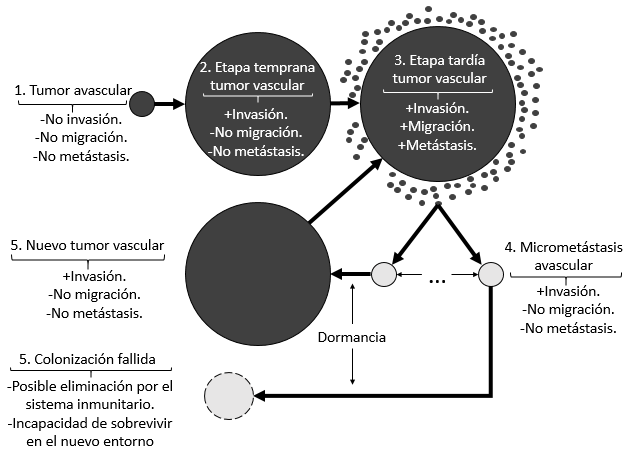
\includegraphics{img/fig-tumor-progresion-2.png}}
\end{center}\vspace*{-0.6cm}
\caption[Ciclo vital del c\'ancer representado por el modelo]{Ciclo vital del c\'ancer representado por el modelo. Como se puede apreciar la \'unica diferencia existente en el modelo entre un tumor primario y uno secundario es su comportamiento durante la etapa avascular, ya que se asume que un tumor primario siempre sobrevive y se desarrolla de forma satisfactoria en su entorno, mientras que una micromet\'astasis puede fallar en colonizar su nuevo entorno o ser destruida por el sistema inmunitario.}
\label{fig-tumor-progresion}
\end{figure}

En la presente secci\'on, referente al surgimiento de c\'elulas tumorales que conforman la masa neopl\'asica, se expone el procedimiento seguido para definir las reglas que reproducen el crecimiento de un tumor primario en ambas etapas y de los tumores secundarios durante la etapa vascular. La transici\'on entre las etapas avascular y vascular en un tumor primario ocurre de forma natural cuando su poblaci\'on celular alcanza cierto punto, mientras que en una met\'astasis esta transici\'on est\'a determinada por un proceso conocido como dormancia o latencia\footnote{De ahora en adelante cuando se utilice la palabra tumor nos estaremos refiriendo a un tumor primario o a un tumor secundario en etapa vascular, salvo que se especifique lo contrario.}. El crecimiento de un tumor secundario durante la etapa avascular y el proceso de dormancia ser\'an expuestas en las secciones~\ref{subsec-micrometastasis} y~\ref{subsec-dormancy}. 

Como se mostr\'o anteriormente la vascularizaci\'on de un tumor es un elemento distintivo de su desarrollo, ya que la difusi\'on de nutrientes permite al propio tumor crecer solo hasta un l\'imite permitido, y es el nuevo suministro de nutrientes proveniente de la neovasculatura la que permite que el tumor contin\'ue su crecimiento m\'as all\'a de dicho l\'imite. Como se mostr\'o en la hip\'otesis VIII sobre el desarrollo tumoral en funci\'on de la poblaci\'on, el modelo asume que la din\'amica de un tumor sigue la funci\'on de crecimiento log\'istico de Verhulst~\cite{verhulst}, presentada a continuaci\'on:
\begin{equation}
\left\lbrace
	\begin{array}{l}		
		\displaystyle\frac{dP}{dt} = rP(1-\displaystyle\frac{P}{K})\vspace*{0.2cm}\\
		P(t=0)=P_0
	\end{array}
\right., \label{eq-verhulst}
\end{equation}
donde se expresa que la variaci\'on de la poblaci\'on respecto al tiempo depende de un ritmo de crecimiento $r$, la poblaci\'on $P$ en ese instante de tiempo y un valor $K$ que representa la capacidad de carga, es decir, la cantidad de individuos de la poblaci\'on que puede sostener el entorno. La angiog\'enesis se puede traducir como un aumento de la capacidad de carga $K$ del entorno, as\'i como un incremento en el ritmo de proliferaci\'on celular debido a que la neovasculatura constituye un m\'etodo de suministro m\'as eficiente que la difusi\'on de nutrientes. Por tanto la din\'amica global del crecimiento ser\'a descrita por dos expresiones: una correspondiente con la etapa avascular y una correspondiente con la etapa vascular, ambas con sus par\'ametros particulares. Como consecuencia del an\'alisis anterior se adopta la siguiente hip\'otesis:

\begin{itemize}
\item [{XIV.}] \textbf{Interpretaci\'on de la neovasculatura}: \emph{Se asume que la neovasculatura que crece en el interior de un tumor producto de la angiog\'enesis produce un aumento en la capacidad de carga del entorno y en el ritmo de proliferaci\'on del propio tumor.} \label{XIV}
\end{itemize} 

En las reglas sobre la conservaci\'on del estado de las c\'elulas normales del aut\'omata~(\ref{eq-inert}) se especific\'o que dichas c\'elulas no cambian de estado salvo que en se encuentren en presencia de c\'elulas cancer\'igenas pertenecientes a alg\'un tumor. Esto significa que la regla del crecimiento tumoral se puede definir a partir de esta condici\'on, es decir, las c\'elulas normales tienen una probabilidad de ser desplazadas de su posici\'on si se encuentran pr\'oximas a una o varias c\'elulas cancer\'igenas pertenecientes a uno o distintos tumores, o en t\'erminos de la funci\'on~(\ref{eq-near-neighbours}) $\mathcal{N}_3^n(S(v,n)) > 0$. Por tanto las reglas se definen de la siguiente forma:
\begin{equation}
s(v,n+1)=\mathcal{R}(S(v,n))=\left\lbrace
	\begin{array}{ll}
		\zeta_0(S(v,n))& \textit{si } s(v,n)=0~\wedge~\mathcal{N}_3^n(S(v,n)) > 0 \\
		\zeta_1(S(v,n))& \textit{si } s(v,n)=1~\wedge~\mathcal{N}_3^n(S(v,n)) > 0 \\
		\zeta_2(S(v,n))& \textit{si } s(v,n)=2~\wedge~\mathcal{N}_3^n(S(v,n)) > 0 
	\end{array}
\right., \label{eq-celldiv}
\end{equation}
donde $\zeta_i(S(v,n)) \in \lbrace i,3 \rbrace$ con $i \in \lbrace 0,1,2 \rbrace$ son variables aleatorias con la siguiente distribuci\'on de probabilidad:
\begin{subequations}
\begin{equation}
P(\zeta_i(S(v,n))=i) = 1 - \rho(S(v,n) \rightarrow 3),
\end{equation}
\begin{equation}
P(\zeta_i(S(v,n))=3) = \rho(S(v,n) \rightarrow 3).
\end{equation}
\end{subequations}

De las expresiones anteriores se infiere que la probabilidad de que una c\'elula normal sea desplazada por una c\'elula cancer\'igena tiene el valor correspondiente con la evaluaci\'on de la probabilidad de transici\'on $\rho(S(v,n) \rightarrow 3)$, mientras que la probabilidad de que permanezca en el estado original es $1-\rho(S(v,n) \rightarrow 3)$. Como un tumor siempre se expande hacia posiciones vecinas ocupadas por c\'elulas normales se puede asegurar que la masa tumoral posee una forma compacta donde cada c\'elula cancer\'igena posee en su vecindad a otras c\'elulas cancer\'igenas, en correspondencia con lo expresado en la hip\'otesis X sobre la adhesi\'on celular. Esta probabilidad de transici\'on, seg\'un la concepci\'on cl\'asica de un aut\'omata celular, debe definirse de forma tal que utilice solamente la informaci\'on de la configuraci\'on local para estimar el valor resultante. En el contexto del presente modelo es necesario que la probabilidad incorpore la informaci\'on relacionada con el modelo de crecimiento log\'istico.

\subsubsection{Proceso de inferencia de la regla}
La concepci\'on cl\'asica de un aut\'omata celular plantea que la funci\'on de transici\'on local solo puede recibir como argumento la configuraci\'on local de la c\'elula $v$ elegida para su actualizaci\'on~\cite{book}. Esto representa una limitaci\'on del modelo cl\'asico ya que no permite reproducir un n\'umero de procesos biol\'ogicos, tecnol\'ogicos y sociales en los que las posibles transiciones dependen de informaci\'on adicional. Entre los posibles ejemplos se encuentra la modelaci\'on de procesos de crecimiento en los que el n\'umero total de individuos y el potencial de reproducci\'on de la especie constituyen factores que influyen positiva o negativamente en la din\'amica poblacional, y como consecuencia en su probabilidad de crecimiento. Ante esta problem\'atica la idea de varios investigadores~\cite{guinot,ruben,ruanxiaoca,ruanxiaodiff} ha sido proponer extensiones del modelo de aut\'omatas celulares para incluir informaci\'on adicional de alguna forma en la funci\'on de transici\'on local. 

En~\cite{guinot} se expone una metodolog\'ia para la inferencia de reglas estoc\'asticas de un aut\'omata celular a partir de modelos continuos. Esta metodolog\'ia nos presenta nociones que pueden ser utilizadas para extender la concepci\'on cl\'asica. En el presente modelo se combina la probabilidad de transici\'on con las diferentes configuraciones locales que pueden darse, es decir, el criterio de selecci\'on de la regla que se debe aplicar en cada caso depende del estado de la configuraci\'on local, mientras que la probabilidad de transici\'on se obtiene a partir del modelo continuo. La adopci\'on de estas ideas es especialmente favorable ya que la funci\'on de transici\'on local y el criterio de selecci\'on de la regla a aplicar se mantienen de acuerdo a la definici\'on cl\'asica, y solo se modifica la probabilidad de transici\'on. Los nuevos argumentos de la probabilidad de transici\'on constituyen dependencias heterog\'eneas de la funci\'on de transici\'on que no est\'an concebidas en la concepci\'on cl\'asica de los aut\'omatas celulares. Se comienza especificando una probabilidad de transici\'on alternativa que reciba la informaci\'on pertinente al modelo continuo~\cite{guinot}.

\begin{definition}
\label{prop-newlocal-func}
Sea una extensi\'on de la funci\'on de transici\'on local definida en~\ref{def-local-func} que incluye una probabilidad de transici\'on alternativa que depende de nuevos argumentos:
\begin{equation}
s(v,n+1) = \mathcal{R}(S(v,n)) = e_i~~\textit{con probabilidad } \rho(\tau(v,n,N_{tum}) \rightarrow e_i), \label{eq-newlocal-func}
\end{equation}
donde $\tau(v,n,N_{tum})$ es una funci\'on que devuelve el tiempo transcurrido relativo al surgimiento del tumor que intenta expandirse hacia $v$ en el instante de tiempo $n$; e.g. si el instante de tiempo en que surgi\'o el tumor en cuesti\'on es $n'$ el tiempo transcurrido relativo es $n_r = n - n'$. 
\end{definition}

El conjunto $N_{tum}$ contiene la informaci\'on correspondiente con los instantes de tiempo en que surgieron los tumores contenidos en la simulaci\'on. Con el objetivo de ilustrar de forma clara el proceso de inferencia se asume durante esta secci\'on que solo existe un tumor expandi\'endose hacia la c\'elula $v$. En la secci\'on que se muestra a continuaci\'on que trata sobre la inclusi\'on de nuevas hip\'otesis al modelo se esclarece esta suposici\'on exponiendo un m\'etodo de resoluci\'on de las distintas situaciones de competencia que pueden surgir entre varios tumores cuando se expanden hacia una misma c\'elula. En el algoritmo~\ref{alg-n-r} se muestra la implementaci\'on de la funci\'on $\tau(v,n,N_{tum})$ a modo de definici\'on donde se tiene en cuenta la suposici\'on hecha anteriormente, $N^n(v)$ es la funci\'on de vecindad inmediata definida en~\ref{def-neighbourhoods}, la funci\'on $tumor(w)$ devuelve el identificador \'unico asociado al tumor al que pertenece $w$ y la funci\'on $s(w,n)$ es el estado de la c\'elula $w$ en el instante de tiempo $n$ definida en~\ref{def-cellstatus}. Aunque funciones como $\tau(v,n,N_{tum})$ pueden ser definidas matem\'aticamente, se prefiere la definici\'on mediante un algoritmo pues brinda informaci\'on adicional sobre la implementaci\'on del aut\'omata celular.

\begin{algorithm}[!ht]
\caption{Definici\'on de la funci\'on $\tau(v,n,N_{tum})$.} \label{alg-n-r}
\KwData{$v, n, N_{tum}$}
\KwResult{$n_r$}
\For{$w \in N^n(v)$}{
	\If{$s(w,n)=3$}{
		$n_r = n - N_{tum}[tumor(w)]$\;
		\Return $n_r$\;}}
\end{algorithm}

Se reescribe la regla de la aparici\'on de c\'elulas tumorales~(\ref{eq-celldiv}) tomando en cuenta la nueva probabilidad de transici\'on alternativa propuesta en~(\ref{prop-newlocal-func}) como:
\begin{equation}
s(v,n+1)=\mathcal{R}(S(v,n))=\left\lbrace
	\begin{array}{ll}
		\zeta_0(\tau(v,n,N_{tum}))& \textit{si } s(v,n)=0~\wedge~\mathcal{N}_3^n(S(v,n)) > 0 \\
		\zeta_1(\tau(v,n,N_{tum}))& \textit{si } s(v,n)=1~\wedge~\mathcal{N}_3^n(S(v,n)) > 0 \\
		\zeta_2(\tau(v,n,N_{tum}))& \textit{si } s(v,n)=2~\wedge~\mathcal{N}_3^n(S(v,n)) > 0 
	\end{array}
\right., \label{eq-celldiv-2}
\end{equation}
donde la distribuci\'on de probabilidad de las variables aleatorias $\zeta_i(\tau(v,n,N_{tum})) \in \lbrace i,3 \rbrace$ con $i \in \lbrace 0,1,2 \rbrace$ quedar\'ia como:
\begin{subequations}
\begin{equation}
P(\zeta_i(\tau(v,n,N_{tum})=i) = 1 - \rho(\tau(v,n,N_{tum}) \rightarrow 3),
\end{equation}
\begin{equation}
P(\zeta_i(\tau(v,n,N_{tum})=3) = \rho(\tau(v,n,N_{tum}) \rightarrow 3).
\end{equation}
\end{subequations}

El c\'alculo de la probabilidad de transici\'on $\rho(\tau(v,n,N_{tum}) \rightarrow 3)$ se define a partir de la ecuaci\'on de crecimiento log\'istico de Verhulst. Primero se debe escribir la ecuaci\'on de crecimiento de forma tal que podamos expresar la variaci\'on de la poblaci\'on desde un instante de tiempo $n$ hacia el instante $n+1$. Para valores peque\~nos de $\Delta t$, la derivada de la ecuaci\'on de crecimiento se puede determinar de forma aproximada como: 
\begin{subequations}
\begin{equation}
\frac{dP(t)}{dt} \approx \frac{P(t+\Delta t) - P(t)}{\Delta t},
\end{equation}
\begin{equation}
P'(t) \approx \frac{P(t+\Delta t) - P(t)}{\Delta t},
\end{equation}
\begin{equation}
\Delta t P'(t) \approx P(t+\Delta t) - P(t),
\end{equation}
\begin{equation}
P(t+\Delta t) - P(t) \approx \Delta t P'(t),
\end{equation}
\end{subequations}
luego si tomamos el tiempo $t$ como una variable discreta, y hacemos $t=n\Delta t$, obtenemos:
\begin{subequations}
\begin{equation}
P(n\Delta +\Delta t) - P(n\Delta t) \approx \Delta t P'(n\Delta t),
\end{equation}
\begin{equation}
P((n+1)\Delta t) - P(n\Delta t) \approx \Delta t P'(n\Delta t). \label{eq-delta}
\end{equation}
\end{subequations}

La expresi\'on~(\ref{eq-delta}) se interpreta como la variaci\'on de la poblaci\'on del tumor entre los instantes de tiempo $n$ y $n+1$ como se puede apreciar en la parte izquierda $P((n+1)\Delta t) - P(n\Delta t)$. El tiempo que transcurre en el modelo continuo entre los instantes de tiempo $n$ y $n+1$ del aut\'omata celular es $\Delta t$. Se infiere de~(\ref{eq-delta}) que la probabilidad de transici\'on $\rho(\tau(v,n,N_{tum})\rightarrow 3)$ se calcula mediante $P'(t)$. A partir de~(\ref{eq-verhulst}), sujeta a la condici\'on inicial, se obtiene~(ver ap\'endice~\ref{app-a} para el proceso de resoluci\'on):
\begin{equation}
P(t) = \frac{P_0 K}{P_0 + (K-P_0)e^{-rt}}, \label{eq-verhulst-solution}
\end{equation} 
cuya derivada $P'(t)$ finalmente tiene la forma~(ver ap\'endice~\ref{app-b} para el proceso de derivaci\'on):
\begin{equation}
P'(t) = \frac{P_0 K r e^{rt}(K-P_0)}{(P_0 e^{rt} + K - P_0)^2}. \label{eq-prob}
\end{equation}

Se expuso anteriormente que la probabilidad de transici\'on $\rho(\tau(v,n,N_{tum}) \rightarrow 3) \in [0,1]$, lo cual no ocurre con la funci\'on $P'(t)$, por lo que es necesario analizar su imagen. Con este objetivo derivamos la funci\'on $P'(t)$ para buscar los puntos estacionarios~(ver ap\'endice~\ref{app-c} para el proceso de derivaci\'on), obteni\'endose: 
\begin{equation}
P''(t) = \frac{P_0 K r^2 e^{rt} (P_0-K)(P_0 e^{rt} + P_0 - K)}{(P_0 e^{rt} + K - P_0)^3},
\end{equation}
donde se infiere que $P'(t)$ posee un m\'aximo cuando:
\begin{equation}
t = \frac{1}{r} \ln\frac{K-P_0}{P_0}, \label{eq-cond-t}
\end{equation}
evaluando $P'(t)$ en este valor de $t$ obtenemos la probabilidad m\'axima de crecimiento:
\begin{equation}
P'\left(t = \frac{1}{r} \ln\frac{K-P_0}{P_0}\right) = \frac{Kr}{4}.
\end{equation}

Por tanto $P'(t)$ alcanza su valor m\'aximo en el punto $(\frac{1}{r} \ln\frac{K-P_0}{P_0}, \frac{Kr}{4})$, donde este valor depende directamente de la capacidad de carga $K$ y del ritmo de crecimiento $r$, devolviendo el intervalo de probabilidad $[0, \frac{Kr}{4}]$. Supongamos que $\rho_{max}$ es el valor m\'aximo de la funci\'on $P'(t)$ en su dominio, de tal forma que $P'(t) \in [0, \rho_{max}]$ sujeto a la condici\'on $\rho_{max} \leq 1$. Despejando la siguiente desigualdad:
\begin{equation}
\frac{K r}{4} \leq \rho_{max},
\end{equation}
se obtiene la condici\'on necesaria para que la funci\'on $P'(t) \in [0,\rho_{max}]$, quedando:
\begin{equation}
r \leq \frac{4 \rho_{max}}{K}. \label{eq-cond-1}
\end{equation}

Mediante la condici\'on~(\ref{eq-cond-1}) se puede asegurar que la probabilidad de crecimiento tumoral que se obtiene mediante la evaluaci\'on de $P'(t)$ pertenece al intervalo $[0,\rho_{max}]$, permitiendo un mecanismo de ajuste del modelo mediante la adecuada selecci\'on de $\rho_{max}$. Este mecanismo de ajuste se sustenta en el hecho de que los modelos de aut\'omatas que se recogen en trabajos anteriores se dividen en dos clases generales: los que reproducen un modelo concebido espec\'ificamente para la reproducci\'on del crecimiento de tumores como~\cite{ruben}, y los que reproducen un modelo general de crecimiento y lo adaptan al caso espec\'ifico del crecimiento de tumores como~\cite{kansal,kansal3,ruanxiaoca}, categor\'ia a la que pertenece el presente trabajo. En el segundo tipo de trabajos es com\'un encontrar este mecanismo en la forma de una probabilidad base como se aprecia en~\cite{kansal}. La condici\'on~\ref{eq-cond-1} est\'a expresada en base a $r$ dado que el valor de $\rho_{max}$ se selecciona a priori y $K$ se determina directamente a partir de la informaci\'on existente acerca del proceso de crecimiento de un tumor, mientras que el proceso de estimar $r$ carece de una metodolog\'ia por lo que es imprescindible poseer la mayor cantidad de informaci\'on acerca de su valor. Las estimaciones de estos valores se llevan a cabo en la secci\'on~\ref{sec-validation}.

A partir de las hip\'otesis VIII y XIV sobre el desarrollo tumoral en funci\'on de la poblaci\'on y la interpretaci\'on de la neovasculatura respectivamente, se infiere que el crecimiento de la poblaci\'on tumoral se describe mediante dos expresiones correspondientes a las etapas avascular y vascular, cada una con sus valores propios del ritmo de crecimiento $r$ y capacidad de carga $K$. Se puede deducir que ambas etapas poseen tambi\'en valores propios de poblaci\'on inicial $P_0$, donde la poblaci\'on inicial de la etapa vascular $P_0^v$ se corresponde con la capacidad de carga del entorno durante la etapa avascular $K_a$, es decir, $K_a = P_0^v$. An\'alogamente se pueden definir a priori valores de probabilidad m\'aximos $\rho_{max}$ para cada una de estas etapas. Finalmente las probabilidades de transici\'on, con $t=n\Delta t$, quedar\'ian como:
\begin{subequations}
\begin{equation}
\rho_a(n\Delta t) = \displaystyle\frac{P_0^a K_a r_a e^{r_a n\Delta t}(K_a-P_0^a)}{(P_0^a e^{r_a n\Delta t} + K_a - P_0^a)^2},
\label{eq-pa}
\end{equation}
\begin{equation}
\rho_v(n\Delta t) = \displaystyle\frac{P_0^v K_v r_v e^{r_v n\Delta t}(K_v-P_0^v)}{(P_0^v e^{r_v n\Delta t} + K_v - P_0^v)^2}.
\label{eq-pv}
\end{equation}
\end{subequations}

Utilizando las expresiones~(\ref{eq-pa},~\ref{eq-pv}) y diferenciando las etapas del desarrollo tumoral en base a un nuevo par\'ametro $n_a$ que indica el per\'iodo de tiempo que dura la etapa avascular, escribimos la probabilidad de transici\'on $\rho(\tau(v,n,N_{tum}) \rightarrow 3)$ como:
\begin{equation}
\rho(\tau(v,n,N_{tum}) \rightarrow 3) = \left\lbrace
	\begin{array}{ll}
		\rho_a(\tau(v,n,N_{tum}) \Delta t)& \textit{si } \tau(v,n,N_{tum}) \leq n_a \\
		\rho_v((\tau(v,n,N_{tum})-n_a) \Delta t)& \textit{si } \tau(v,n,N_{tum}) > n_a
	\end{array}
\right.. \label{eq-generaldivrule}
\end{equation}

N\'otese en la expresi\'on para el c\'alculo de $\rho_v$ que el tiempo que se utiliza como par\'ametro es el relativo al inicio de la etapa vascular, es decir, $\tau(v,n,N_{tum})-n_a$. La expresi\'on~(\ref{eq-generaldivrule}) se conoce como probabilidad de transici\'on general del crecimiento tumoral y se utiliza como base para la definici\'on de las probabilidades particulares para el desplazamiento de cada tipo de c\'elula normal del aut\'omata. En los segmentos siguientes se exponen las hip\'otesis del modelo que se relacionan con las direcciones de expansi\'on y el crecimiento del tumor hacia distintos tipos de tejidos.

\subsubsection{Inclusi\'on de nuevas hip\'otesis}
El uso de la probabilidad de transici\'on~(\ref{eq-generaldivrule}) en esta forma tiene dos inconvenientes. El primero es que solo tiene en cuenta un tumor expandi\'endose hacia la posici\'on de la c\'elula $v$ como hab\'iamos supuesto anteriormente. En varias circunstancias se pueden dar situaciones donde dos o varios tumores compiten por expandirse hacia una misma posici\'on, es decir, que una c\'elula normal posea en su vecindad inmediata varias c\'elulas cancer\'igenas pertenecientes a distintos tumores cuyas descendencias intentan ocupar la posici\'on de la c\'elula normal. Esta competencia tiene que ser reflejada de alguna forma en la regla del crecimiento tumoral. El segundo es que la probabilidad de transici\'on est\'a expresada solamente en funci\'on de $\rho_a(n\Delta t)$ y $\rho_v(n\Delta t)$ y no incorpora la influencia de otros factores en el crecimiento. Un ejemplo de estos factores es la direcci\'on de la expansi\'on. Se ha demostrado en varias investigaciones que un tumor tiende a crecer en direcci\'on de donde provienen los nutrientes~\cite{kansal3} lo que constituye un sesgo en la direcci\'on de la expansi\'on. Este \'ultimo hecho representa, adem\'as, un factor importante en la direcci\'on de la migraci\'on de las c\'elulas cancer\'igenas durante la cascada metast\'asica~\cite{kansal3}. Otro ejemplo es la velocidad de expansi\'on tumoral. Dada la configuraci\'on de vecindad utilizada las c\'elulas vecinas de una c\'elula central no se encuentran a la misma distancia. Si se toma que la velocidad m\'axima de expansi\'on tumoral representada en el modelo se corresponde con ocupar una celda del aut\'omata de un instante de tiempo al otro, esta velocidad no puede ser la misma si la expansi\'on proviene de una c\'elula vecina a una distancia menor que si proviniese desde una c\'elula vecina a una distancia mayor. Esta situaci\'on se representa en la figura~\ref{fig-expansion-velocity}. La regla general del crecimiento tumoral no toma en cuenta estos factores, por lo que es necesaria su inclusi\'on. Comenzamos planteando las siguientes hip\'otesis del modelo:
\begin{figure}[!ht]
\begin{center}
\scalebox{0.45}{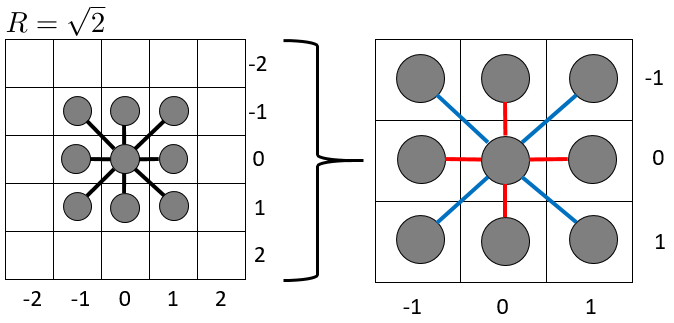
\includegraphics{img/fig-expansion-velocity.png}}
\end{center}\vspace*{-0.6cm}
\caption[Representaci\'on de las distintas velocidades de expansi\'on representadas en el modelo seg\'un la configuraci\'on de vecindad utilizada]{Representaci\'on de las distintas velocidades de expansi\'on representadas en el modelo seg\'un la configuraci\'on de vecindad utilizada. Las l\'ineas rojas en el diagrama derecho indican una mayor velocidad de expansi\'on que las l\'ineas azules. Esta noci\'on de velocidad se basa en la distancia entre estas c\'elulas.}
\label{fig-expansion-velocity}
\end{figure}

\begin{itemize}
\item [{XV.}] \textbf{Situaciones de competencia tumorales}: \emph{En las situaciones de competencia de varios tumores por expandirse a una misma posici\'on se asume que el valor de la probabilidad de transici\'on se corresponde con el tumor con mayor probabilidad de expansi\'on en ese momento. Si el tumor finalmente se expande hacia dicha posici\'on de forma satisfactoria, la nueva c\'elula cancer\'igena pertenece a dicho tumor.} \label{XV}

\item [{XVI.}] \textbf{Vectores de concentraci\'on de nutrientes}: \emph{Se asume que la concentraci\'on de nutrientes aumenta a medida que nos aproximamos a los tejidos de sost\'en y a la vasculatura del organismo. Este hecho se representa mediante uno o varios vectores en los \'organos del conjunto de c\'elulas del aut\'omata que indica las direcciones en que aumenta la concentraci\'on de los nutrientes.} \label{XVI}

\item [{XVII.}] \textbf{Sesgo direccional del crecimiento tumoral}: \emph{Se asume que la probabilidad de que aumente la poblaci\'on celular de un tumor se ve afectada por la concentraci\'on de los nutrientes. Este hecho constituye un sesgo en la direcci\'on del crecimiento del tumor, que se traduce en la tendencia a expandirse hacia la mayor concentraci\'on.} \label{XVII}

\item [XVIII.] \textbf{Velocidad de expansi\'on tumoral:} \emph{Se asume que la velocidad de expansi\'on tumoral depende de la distancia entre las c\'elulas tumorales y la c\'elula sana que intentan desplazar, que disminuye a medida que aumenta la distancia.} \label{XVIII}
\end{itemize}

Debe aclararse que la hip\'otesis XV tiene su fundamento biol\'ogico en que las cercan\'ias de una neoplasia con cierto grado de desarrollo la concentraci\'on de nutrientes es menor que en un tejido sano pues la masa tumoral consume una parte importante de los mismos. Luego cualquier tumor con un desarrollo inferior, en especial uno que posee un bajo grado o nulo de vascularizaci\'on, no tiende a expandirse hacia un tumor mayor que acapara la mayor parte de los nutrientes provenientes de la difusi\'on. Esta suposici\'on se refuerza con la hip\'otesis XVII y con la naturaleza oportunista y autorregulada del crecimiento tumoral. La hip\'otesis XVII permite explicar la expansi\'on del tumor en las distintas capas de tejidos que conforman los \'organos. Los tumores s\'olidos tienden a penetrar el estroma en busca de estos nutrientes a pesar de que presentan una mayor densidad, raz\'on por la que apenas crecen hacia el lumen del \'organo aunque presente una densidad nula. Con el objetivo de representar estas nuevas hip\'otesis del modelo es necesario reescribir la definici\'on de la probabilidad de transici\'on alternativa~(\ref{prop-newlocal-func}) como se muestra a continuaci\'on:

\begin{definition}
\label{prop-newlocal-func-2}
La funci\'on de transici\'on local definida en~\ref{prop-newlocal-func} se reescribe obteni\'endose una probabilidad de transici\'on alternativa que depende de nuevos argumentos:
\begin{equation}
s(v,n+1) = \mathcal{R}(S(v,n)) = e_i~~\textit{con probabilidad } \rho(\tau(v,n,N_{tum}) \rightarrow e_i), \label{eq-newlocal-func-2}
\end{equation}
donde $\tau(v,n,N_{tum})$ es una funci\'on que devuelve el conjunto de todos los tiempos transcurridos relativos al surgimiento de los tumores que intentan expandirse hacia $v$ en el instante de tiempo $n$; e.g. si los instantes de tiempo en que surgieron los tumores en cuesti\'on conforman el conjunto $\lbrace n_1', n_2', \ldots, n_m' \rbrace$ con $m$ la cantidad de tumores, el conjunto de tiempos transcurridos relativos es $n_r = \lbrace n-n_1',n-n_2', \ldots, n-n_m' \rbrace$.
\end{definition}

En el algoritmo~\ref{alg-n-r-2} se muestra la implementaci\'on de la nueva funci\'on $\tau(v,n,N_{tum})$ a modo de definici\'on donde se tiene en cuenta la hip\'otesis XV sobre las situaciones de competencia tumorales, $N^n(v)$ es la funci\'on de vecindad inmediata definida en~\ref{def-neighbourhoods}, la funci\'on $tumor(w)$ devuelve el identificador \'unico asociado al tumor al que pertenece $w$ y la funci\'on $s(w,n)$ es el estado de la c\'elula $w$ en el instante de tiempo $n$ definida en~\ref{def-cellstatus}. Se reescribe la regla del crecimiento tumoral~(\ref{eq-celldiv-2}) tomando en cuenta la nueva probabilidad de transici\'on alternativa~(\ref{eq-newlocal-func-2}) como:
\begin{equation}
s(v,n+1)=\mathcal{R}(S(v,n))=\left\lbrace
	\begin{array}{ll}
		\zeta_0(\tau(v,n,N_{tum}))& \textit{si } s(v,n)=0~\wedge~\mathcal{N}_3^n(S(v,n)) > 0 \\
		\zeta_1(\tau(v,n,N_{tum}))& \textit{si } s(v,n)=1~\wedge~\mathcal{N}_3^n(S(v,n)) > 0 \\
		\zeta_2(\tau(v,n,N_{tum}))& \textit{si } s(v,n)=2~\wedge~\mathcal{N}_3^n(S(v,n)) > 0 
	\end{array}
\right., \label{eq-celldiv-3}
\end{equation}
donde la distribuci\'on de probabilidad de las variables aleatorias $\zeta_i(\tau(v,n,N_{tum})) \in \lbrace i,3 \rbrace$ con $i \in \lbrace 0,1,2 \rbrace$ quedar\'ia como:
\begin{subequations}
\begin{equation}
P(\zeta_i(\tau(v,n,N_{tum}))=i) = 1 - \rho(\tau(v,n,N_{tum}) \rightarrow 3),
\end{equation}
\begin{equation}
P(\zeta_i(\tau(v,n,N_{tum}))=3) = \rho(\tau(v,n,N_{tum}) \rightarrow 3).
\end{equation}
\end{subequations}

\begin{algorithm}[t]
\caption{Definici\'on de la funci\'on $\tau(v,n,N_{tum})$.} \label{alg-n-r-2}
\KwData{$v, n, N_{tum}$}
\KwResult{$n_r$}
$n_r = \lbrace \rbrace$\;
\For{$w \in N^n(v)$}{
	\If{$s(w,n)=3$}{
		$n' = n - N_{tum}[tumor(w)]$\;
		$n_r = n_r \cup \lbrace n' \rbrace$\;}}
\Return $n_r$\;
\end{algorithm}

De acuerdo a la hip\'otesis XV sobre situaciones de competencia tumorales, la probabilidad de transici\'on~(\ref{eq-generaldivrule}) debe depender de las probabilidades de expansi\'on de cada uno de los tumores cuyos tiempos transcurridos relativos se encuentran en $\tau(v,n,N_{tum})$. Como se adopta la norma general que solo se expande el tumor con mayores posibilidades esta probabilidad de transici\'on puede ser escrita, tomando en cuenta la definici\'on~(\ref{prop-newlocal-func-2}), como:
\begin{equation}
\rho(\tau(v,n,N_{tum}) \rightarrow 3) = max\left[\rho(n_1 \rightarrow 3),\rho(n_2 \rightarrow 3),\ldots, \rho(n_m \rightarrow 3)\right], \label{eq-generaldivrule-2}
\end{equation}
donde $n_i \in \tau(v,n,N_{tum})$ con $i \in \lbrace 1,2,\ldots,m \rbrace$ y $m=|\tau(v,n,N_{tum})|$. La funci\'on $\rho(n_i \rightarrow 3)$ es la aplicaci\'on individual de la probabilidad de transici\'on a cada tumor contenido en el conjunto devuelto por la funci\'on $\tau(v,n,N_{tum})$. Se puede apreciar que el valor de la probabilidad de transici\'on global se corresponde con el m\'aximo de las probabilidades de expansi\'on de cada uno de los tumores que compiten por la posici\'on de la c\'elula $v$. La aplicaci\'on particular se escribe a partir de la probabilidad de transici\'on general del crecimiento tumoral~(\ref{eq-generaldivrule}):
\begin{equation}
\rho(n_i \rightarrow 3) = \left\lbrace
	\begin{array}{ll}
		\rho_a(n_i \Delta t)& \textit{si } n_i \leq n_a \\
		\rho_v((n_i - n_a) \Delta t)& \textit{si } n_i > n_a
	\end{array}
\right.. \label{eq-generaldivrule-3}
\end{equation}

Continuando con el proceso de incorporaci\'on de nuevas hip\'otesis a la probabilidad de transici\'on general del crecimiento tumoral, la hip\'otesis XVII sobre el sesgo direccional del crecimiento tumoral indica que la expansi\'on de un tumor tiende a producirse hacia una mayor concentraci\'on de nutrientes. Con el objetivo de simular la variaci\'on de dicha concentraci\'on en el tejido y tomando en cuenta la hip\'otesis XVI sobre los vectores de concentraci\'on de nutrientes se plantean las siguientes definiciones:

\begin{definition}
\label{def-regions}
Una regi\'on se define como:
\begin{equation}
R_i = \lbrace v~|~v \in V(G) : (x_{min} \leq v_x < x_{max})~\wedge~(y_{min} \leq v_y < y_{max}) \rbrace,
\end{equation}
donde $x_{min}$ y $y_{min}$ son los valores extremos inferiores de la regi\'on definida, mientras que $x_{max}$ y $y_{max}$ son los valores extremos superiores de la regi\'on definida. Las regiones definidas constituyen una partici\'on del conjunto de v\'ertices del grafo $V(G)$.
\end{definition}

\begin{definition}
\label{def-concentration}
Un vector de concentraci\'on expresa una direcci\'on hacia la cual aumenta el valor de la disponibilidad de nutrientes, tomando como regla general que el aumento ocurre en direcci\'on a los tejidos de sost\'en y a su vasculatura. Para simular condiciones heterog\'eneas en el interior de los \'organos cada uno de estos vectores est\'a asociado a una y solo una regi\'on dentro del mismo. El conjunto de vectores de concentraci\'on se denota como $B$, donde $B_i$ es el conjunto de vectores asociados al \'organo $i$ y $B_{ij}$ es el conjunto de vectores asociados al \'organo $i$ y a la regi\'on $R_j$ que pertenece a ese \'organo. 
\end{definition}

Por ejemplo en los diagramas izquierdo y centro de los cortes de tejidos mostrados en la figura~\ref{fig-structure} correspondientes con el aparato digestivo y las v\'ias a\'ereas inferiores del sistema respiratorio la variaci\'on de la concentraci\'on de nutrientes se puede representar mediante un vector que parte desde el tejido epitelial y apunta perpendicularmente hacia el estroma. En el caso del diagrama derecho de la figura~\ref{fig-structure} correspondiente con el h\'igado no hay necesidad de representar ning\'un vector ya que la vasculatura est\'a presente de manera uniforme en el \'organo haciendo de la concentraci\'on de nutrientes una magnitud homog\'enea. 

Generalmente se utiliza la similitud coseno para determinar el grado de similitud existente entre dos vectores mediante el valor del coseno del menor \'angulo comprendido entre ellos. En el presente trabajo se eval\'uan las similitudes coseno entre todos los vectores del conjunto $B$ que pertenecen a la regi\'on donde se localiza el tumor y el vector formado entre el centroide del tumor y la c\'elula $v$ hacia el que se est\'a expandiendo, tomando la mayor similitud como medida. Se interpreta esta medida como un coeficiente de las probabilidades de transici\'on de cada etapa del tumor $\rho_a(n \Delta t)$ y $\rho_v(n \Delta t)$, de manera el crecimiento se ve sesgado hacia la mayor concentraci\'on de nutrientes. A partir de lo expuesto anteriormente se plantean las siguientes definiciones:

\begin{definition}
\label{def-general-vector}
Sean dos c\'elulas $v$ y $w$ del conjunto $V(G)$. Un vector $\overrightarrow{\nu_{vw}}$ entre las c\'elulas $v$ y $w$ se define como:
\begin{equation}
\overrightarrow{\nu_{vw}} = \left(v_x - w_x, v_y - w_y \right). \label{eq-general-vector}
\end{equation}
\end{definition}

\begin{definition}
\label{def-sim}
Sean dos vectores $\overrightarrow{\nu_1}$ y $\overrightarrow{\nu_2}$, se define la similitud coseno $\beta(\overrightarrow{\nu_1},\overrightarrow{\nu_2})$ como el coseno del menor \'angulo, denotado como $\alpha$, comprendido entre ellos y se determina como:
\begin{equation}
\beta(\overrightarrow{\nu_1},\overrightarrow{\nu_2}) = \cos \alpha = \displaystyle\frac{\overrightarrow{\nu_1} \cdot \overrightarrow{\nu_2}}{|\overrightarrow{\nu_1}| \times |\overrightarrow{\nu_2}|}. \label{eq-sim}
\end{equation}
Como siempre toma el menor \'angulo comprendido entre los vectores, el mayor \'angulo comprendido posible es $\pi$ donde la similitud toma valor $-1$, que es el caso donde ambos vectores tienen direcciones opuestas. El menor \'angulo comprendido es $0$ donde la similitud toma valor $1$, correspondiente con el caso donde ambos vectores apuntan hacia la misma direcci\'on. La similitud toma valor $0$ cuando el \'angulo es $\pi /2$. Luego los valores posibles de la similitud coseno son:
\begin{equation}
\beta(\overrightarrow{\nu_1},\overrightarrow{\nu_2}) = \cos \alpha \in \left\lbrace
	\begin{array}{ll}
		\left[0,~1\right]& \textit{si } \alpha \in \left[0,\frac{\pi}{2} \right)\\
		\left[\textit{-}1,0\right]& \textit{si } \alpha \in \left[\frac{\pi}{2}, \pi \right]
	\end{array}
\right..
\end{equation}
\end{definition}

Como podemos apreciar, el valor de la similitud oscila entre $-1$ y $1$. La interpretaci\'on de los valores negativos puede ser inadecuada al ser utilizados como un coeficiente de probabilidad. Con el objetivo de penalizar el crecimiento tumoral contrario a los vectores de concentraci\'on de nutrientes y favorecerlo cuando dicho crecimiento ocurre en la misma direcci\'on se opta por utilizar una aplicaci\'on lineal que transforme el intervalo $[-1,1]$ de los valores de la similitud en el intervalo $[0$.$5, 1$.$5]$. De esta forma se penaliza la probabilidad de expansi\'on al multiplicarse por $0$.$5$ si este crecimiento es contrario a la direcci\'on indicada por los vectores de concentraci\'on, o se favorece al multiplicarse por $1$.$5$ si ocurre en la misma direcci\'on que la indicada por los vectores de concentraci\'on. De esta forma se mantiene el balance del crecimiento tumoral. En caso de que una probabilidad tome un valor mayor que $1$ al ser multiplicado por alg\'un coeficiente definido en el presente modelo su valor se hace igual a $1$. Se debe aclarar que si se toma el valor $0$ como penalizaci\'on del crecimiento tumoral negar\'ia la posibilidad de expansi\'on contraria a la direcci\'on indicada por los vectores de concentraci\'on de nutrientes. Esta nueva similitud alternativa se define a continuaci\'on:

\begin{definition}
\label{def-simprima}
Sean dos vectores $\overrightarrow{\nu_1}$ y $\overrightarrow{\nu_2}$, se define la similitud coseno alternativa $\beta_{alt}(\overrightarrow{\nu_1},\overrightarrow{\nu_2})$ como:
\begin{equation}
\beta_{alt}(\overrightarrow{\nu_1},\overrightarrow{\nu_2}) = \frac{1}{2} \beta(\overrightarrow{\nu_1},\overrightarrow{\nu_2}) + 1. \label{eq-simprima}
\end{equation}
La similitud coseno alternativa $\beta_{alt}(\overrightarrow{\nu_1},\overrightarrow{\nu_2}) \in [0$.$5, 1$.$5]$ cuando $\beta(\overrightarrow{\nu_1},\overrightarrow{\nu_2}) \in [-1, 1]$. 
\end{definition}

A partir de la expresi\'on~\ref{eq-simprima} se declara el coeficiente de la probabilidad de transici\'on $\beta_{tum}(v,l)$ como se muestra a continuaci\'on:

\begin{definition}
\label{def-beta}
La funci\'on $\beta_{tum}(v,l)$, que recibe una c\'elula $v$ y un tumor $l$, devuelve la m\'axima similitud coseno alternativa entre el vector $\overrightarrow{\nu_{vl}}$ y cada uno de los vectores de concentraci\'on del conjunto $B$ que pertenecen al mismo \'organo que el tumor $l$, es decir:
\begin{equation}
\beta_{tum}(v,l) = max\left[\beta_{alt}(\overrightarrow{b_{ij1}},\overrightarrow{\nu_{vl}}),\,\beta_{alt}(\overrightarrow{b_{ij2}}, \overrightarrow{\nu_{vl}})\,,\ldots,\,\beta_{alt}(\overrightarrow{b_{ijm}}, \overrightarrow{\nu_{vl}})\right], \label{eq-beta}
\end{equation}
donde $\overrightarrow{b_{ijk}} \in B_{ij}$ con $k \in \lbrace 1,2,\cdots,m \rbrace$ y $m=|B_{ij}|$ son los vectores de concentraci\'on asociados a la regi\'on $R_j$ del \'organo $i$ a la que pertenece la c\'elula $v$, o sea, $v \in R_j$, y $\overrightarrow{\nu_{vl}}$ es el vector formado por el c\'elula $v$ y el centroide del tumor $l$, donde el centroide constituye el punto de aplicaci\'on y $v$ el extremo del vector. 
\end{definition}

Las definiciones de un vector de expansi\'on y del centroide del tumor se presentan a continuaci\'on:

\begin{definition}
\label{def-centroid}
Sea $l=\lbrace w_1,w_2,\ldots,w_{m}\rbrace$ con $m=|l|$ un conjunto que contiene las c\'elulas pertenecientes a un tumor cualquiera representado en el aut\'omata. El centroide de dicho tumor se denota como $c_l$ y se define como el promedio de las componentes de las c\'elulas del conjunto, es decir:
\begin{equation}
c_l = \left(\frac{w_{1x} + w_{2x} + \ldots + w_{mx}}{m}, \frac{w_{1y} + w_{2y} + \ldots + w_{my}}{m} \right). \label{eq-centroid}
\end{equation}
\end{definition}

\begin{definition}
\label{def-exp-vector}
Sea el centroide $c_l$ de un tumor cualquiera $l$ y una c\'elula $v$ hacia el que se est\'a expandiendo dicho tumor. A partir de la expresi\'on~(\ref{eq-general-vector}) se define el vector de expansi\'on $\overrightarrow{\nu_{vl}}$ entre el centroide del tumor $c_l$ y la c\'elula $v$ como:
\begin{equation}
\overrightarrow{\nu_{vl}} = \left(v_x - c_{lx}, v_y - c_{ly} \right). \label{eq-exp-vector}
\end{equation}
\end{definition}

Seg\'un la hip\'otesis XVIII la velocidad de expansi\'on tumoral depende de la distancia a la que se encuentran las c\'elulas tumorales de las c\'elulas normales que intentan desplazar. La noci\'on consiste en tomar la mayor velocidad de entre todas las c\'elulas tumorales pertenecientes a un mismo tumor presentes en la vecindad de la c\'elula normal. Para este fin se definen las siguientes funciones:

\begin{definition}
\label{def-tumor-neighbourhood}
La funci\'on $N(v,l)$, que recibe una c\'elula normal $v$ y un tumor $l$, devuelve el conjunto de c\'elulas vecinas inmediatas de $v$ tales que pertenecen al tumor $l$ y que pertenezcan al mismo \'organo, es decir:
\begin{equation}
N(v,l) = \lbrace w~|~w \in \mathcal{N}^n(v)~\wedge~w \in l~\wedge~V_v(G) = V_w(G) \rbrace. \label{eq-tumor-neighbourhood}
\end{equation}
\end{definition}

\begin{definition}
\label{def-tumor-velocity}
La funci\'on $\gamma(v,w)$, que recibe una c\'elula normal $v$ y una tumoral $w$, devuelve la velocidad de expansi\'on tumoral en dependencia de la distancia euclideana~(Def. \ref{def-euclidean-distance}) existente entre ellas, es decir:
\begin{equation}
\gamma(v,w) = \left\lbrace
	\begin{array}{ll}
		0$.$5 & \textit{si } d_E(v,w) > 1 \\
		1$.$5 & \textit{si } d_E(v,w) = 1 
	\end{array}
\right.. \label{eq-tumor-velocity}
\end{equation}
\end{definition}

A partir de la expresi\'on~\ref{eq-tumor-velocity} se declara el coeficiente de la velocidad de expansi\'on tumoral $\gamma_{tum}(v,N(v,l))$ como se muestra a continuaci\'on:

\begin{definition}
\label{def-velocity-function}
La funci\'on $\gamma_{tum}(v,N(v,l))$, que recibe una c\'elula normal $v$ y las c\'elulas vecinas a esta $N(v,l)$ que pertenecen al tumor $l$, devuelve el m\'aximo valor de velocidad entre la c\'elula normal $v$ y cada una de las c\'elulas tumorales vecinas que pertenecen al conjunto $N(v,l)$, es decir:
\begin{equation}
\gamma_{tum}(v,N(v,l)) = max\left[\gamma(v,w_1), \gamma(v,w_2), \ldots \gamma(v,w_m) \right], \label{eq-velocity-function}
\end{equation}
donde $w_i \in N(v,l)$ con $i \in \lbrace 1,2,\cdots,m \rbrace$ y $m=|N(v,l)|$.
\end{definition}

Hasta el momento se han definido dos nuevos coeficientes de sesgo direccional del crecimiento tumoral $\beta_{tum}(v,l)$ y $\gamma_{tum}(v,N(v,l))$ que se desean incluir a la aplicaci\'on particular de la probabilidad de transici\'on general de la divisi\'on celular expuesta en~(\ref{eq-generaldivrule-3}). Con el objetivo de representar estas nuevas hip\'otesis del modelo es necesario reescribir la definici\'on de la probabilidad de transici\'on~(\ref{prop-newlocal-func-2}) como se muestra a continuaci\'on:

\begin{definition}
\label{prop-newlocal-func-2-1}
La funci\'on de transici\'on local definida en~\ref{prop-newlocal-func-2} se reescribe obteni\'endose una probabilidad de transici\'on alternativa que depende de nuevos argumentos:
\begin{equation}
s(v,n+1) = \mathcal{R}(S(v,n)) = e_i~~\textit{con probabilidad } \rho(v,\tau(v,n,N_{tum},L_{tum}) \rightarrow e_i), \label{eq-newlocal-func-2-1}
\end{equation}
donde $\tau(v,n,N_{tum},L_{tum})$ es una funci\'on que devuelve un conjunto compuesto por tuplas correspondientes con cada tumor que intenta expandirse hacia $v$ en el instante de tiempo $n$ que contienen el tiempo transcurrido relativo al surgimiento de dicho tumor y el conjunto de c\'elulas que lo conforman. El conjunto $L_{tum}$ contiene la informaci\'on correspondiente con los conjuntos de c\'elulas que conforman los tumores contenidos en la simulaci\'on.
\end{definition}

En el algoritmo~\ref{alg-L-c} se muestra la implementaci\'on de la funci\'on $\tau(v,n,N_{tum},L_{tum})$ a modo de definici\'on donde $N^n(v)$ es la funci\'on de vecindad inmediata definida en~\ref{def-neighbourhoods}, la funci\'on $tumor(w)$ devuelve el identificador \'unico asociado al tumor al que pertenece $w$ y la funci\'on $s(w,n)$ es el estado de la c\'elula $w$ en el instante de tiempo $n$ definida en~\ref{def-cellstatus}.

\begin{algorithm}[!ht]
\caption{Definici\'on de la funci\'on $\tau(v,n,N_{tum},L_{tum})$.} \label{alg-L-c}
\KwData{$v, n, N_{tum}, L_{tum}$}
\KwResult{$L$}
$L = \lbrace \rbrace$\;
\For{$w \in N^n(v)$}{
	\If{$s(w,n)=3$}{
		$l = L_{tum}[tumor(w)]$\;
		$n_r = n - N_{tum}[tumor(w)]$\;
		$L = L \cup \lbrace \langle n_r, l \rangle \rbrace$\;}}
\Return $L$\;
\end{algorithm}

Se reescribe la regla del crecimiento tumoral~(\ref{eq-celldiv-3}) tomando en cuenta la nueva probabilidad de transici\'on alternativa~(\ref{eq-newlocal-func-2-1}) como:
\begin{equation}
s(v,n+1)=\mathcal{R}(S(v,n))=\left\lbrace
	\begin{array}{ll}
		\zeta_0(v,\tau(v,n,N_{tum},L_{tum}))& \textit{si } s(v,n)=0~\wedge~\mathcal{N}_3^n(S(v,n)) > 0\\
		\zeta_1(v,\tau(v,n,N_{tum},L_{tum}))& \textit{si } s(v,n)=1~\wedge~\mathcal{N}_3^n(S(v,n)) > 0\\
		\zeta_2(v,\tau(v,n,N_{tum},L_{tum}))& \textit{si } s(v,n)=2~\wedge~\mathcal{N}_3^n(S(v,n)) > 0 \\
	\end{array}
\right., \label{eq-celldiv-3-1}
\end{equation}
donde la distribuci\'on de probabilidad de las variables aleatorias $\zeta_i(v,\tau(v,n,N_{tum},L_{tum}))$ $\in \lbrace i,3 \rbrace$ con $i \in \lbrace 0,1,2 \rbrace$ quedar\'ia como:
\begin{subequations}
\begin{align}
P(\zeta_i(v,\tau(v,n,N_{tum},L_{tum}))=i) &= 1 - \rho(v,\tau(v,n,N_{tum},L_{tum}) \rightarrow 3),\\
P(\zeta_i(v,\tau(v,n,N_{tum},L_{tum}))=3) &= \rho(v,\tau(v,n,N_{tum},L_{tum}) \rightarrow 3).
\end{align}
\end{subequations}

La probabilidad de transici\'on $\rho(v,\tau(v,n,N_{tum},L_{tum}) \rightarrow 3)$ se escribe de forma an\'aloga a la expresi\'on~(\ref{eq-generaldivrule-2}) de acuerdo a la hip\'otesis XV sobre situaciones de competencia tumorales y tomando en cuenta la definici\'on~(\ref{prop-newlocal-func-2-1}), como:
\begin{equation}
\rho(v,\tau(v,n,N_{tum},L_{tum}) \rightarrow 3) = max\left[\rho(v, n_1, l_1 \rightarrow 3),\rho(v, n_2, l_2 \rightarrow 3),\ldots, \rho(v, n_m, l_m \rightarrow 3)\right], \label{eq-generaldivrule-2-1}
\end{equation}
donde $n_i$ y $l_i$ son los valores de la tupla $\langle n_i, l_i \rangle \in \tau(v,n,N_{tum},L_{tum})$ con $i \in \lbrace 1,2,\ldots,m \rbrace$ y $m=|\tau(v,n,N_{tum},L_{tum})|$ correspondiente con el i-\'esimo tumor que se intenta expandir hacia $v$. La funci\'on $\rho(v, n_i, l_i \rightarrow 3)$ es la aplicaci\'on individual de la probabilidad de transici\'on a cada tumor contenido en el conjunto devuelto por la funci\'on $\tau(v,n,N_{tum},L_{tum})$. A partir de las expresiones~(\ref{eq-generaldivrule-2-1},~\ref{eq-beta},~\ref{eq-velocity-function}) se reescribe la aplicaci\'on particular de la probabilidad de transici\'on general de la divisi\'on celular como:
\begin{equation}
\rho(v,n_i,l_i \rightarrow 3) = \left\lbrace
	\begin{array}{ll}
		\gamma_{tum}(v,N(v,l_i))\,\beta_{tum}(v,l_i)\,\rho_a(n_i \Delta t)& \textit{si } n_i \leq n_a \\
		\gamma_{tum}(v,N(v,l_i))\,\beta_{tum}(v,l_i)\,\rho_v((n_i - n_a) \Delta t)& \textit{si } n_i > n_a
	\end{array}
\right.. \label{eq-generaldivrule-2-2}
\end{equation}

Finalmente, la probabilidad de transici\'on general del crecimiento tumoral representa los desplazamientos de las c\'elulas normales de su posici\'on por las c\'elulas cancer\'igenas pertenecientes a la masa tumoral, reproduciendo las distintas situaciones de competencia entre tumores, los sesgos direccionales basados en la concentraci\'on de nutrientes y las velocidades de expansi\'on tumoral. No obstante, en esta forma general no describe todav\'ia las mec\'anicas espec\'ificas de expansi\'on tumoral hacia los distintos tipos de tejidos. Es necesario especificar el c\'alculo de dicha probabilidad seg\'un el tipo de c\'elula normal desplazada.

\subsubsection{Probabilidades de transici\'on particulares}
Hasta el momento se ha definido una probabilidad de transici\'on del crecimiento tumoral de forma general, pero es bien conocido que la invasi\'on de distintos tipos de tejidos normales ocurre bajo condiciones espec\'ificas. Dados los distintos tipos de c\'elulas normales representadas en el aut\'omata se deben describir cuales son las condiciones que provocan la penetraci\'on de los tejidos conformados por dichas c\'elulas. Como se expuso al comienzo de la presente secci\'on un tumor primario durante la etapa avascular es incapaz de invadir los tejidos de sost\'en pero su expansi\'on puede ocurrir dentro del epitelio donde se origin\'o y hacia el lumen, donde ambos procesos est\'an bajo la influencia del sesgo direccional basados en los vectores de concentraci\'on de nutrientes. Es durante la etapa vascular que gana la posibilidad de invadir el estroma producto de la angiog\'enesis. Un tumor secundario durante la etapa vascular tiene la capacidad de invadir el lumen, el epitelio y los tejidos de sost\'en del \'organo, ya que constituyen la evoluci\'on de una micromet\'astasis que pose\'ia de antemano dichas capacidades. Las distribuciones de probabilidad de las variables aleatorias $\zeta_0(v,\tau(v,n,N_{tum},L_{tum}))$, $\zeta_1(v,\tau(v,n,N_{tum},L_{tum}))$ y $\zeta_2(v,\tau(v,n,N_{tum},L_{tum}))$ est\'an planteadas en funci\'on de la probabilidad de transici\'on general definida en~(\ref{eq-generaldivrule-2-2}), pero seg\'un las descripciones anteriores es necesario escribir de forma particular cada probabilidad de transici\'on seg\'un el tipo de c\'elula desplazada. Luego la distribuci\'on de probabilidad de estas variables aleatorias quedar\'ia como:
\begin{subequations}
\begin{align}
P(\zeta_0(v,\tau(v,n,N_{tum},L_{tum}))=0) &= 1 - \rho_0(v,\tau(v,n,N_{tum},L_{tum}) \rightarrow 3),\\
P(\zeta_0(v,\tau(v,n,N_{tum},L_{tum}))=3) &= \rho_0(v,\tau(v,n,N_{tum},L_{tum}) \rightarrow 3),\\
P(\zeta_1(v,\tau(v,n,N_{tum},L_{tum}))=1) &= 1 - \rho_1(v,\tau(v,n,N_{tum},L_{tum}) \rightarrow 3),\\
P(\zeta_1(v,\tau(v,n,N_{tum},L_{tum}))=3) &= \rho_1(v,\tau(v,n,N_{tum},L_{tum}) \rightarrow 3),\\
P(\zeta_2(v,\tau(v,n,N_{tum},L_{tum}))=2) &= 1 - \rho_2(v,\tau(v,n,N_{tum},L_{tum}) \rightarrow 3),\\
P(\zeta_2(v,\tau(v,n,N_{tum},L_{tum}))=3) &= \rho_2(v,\tau(v,n,N_{tum},L_{tum}) \rightarrow 3),
\end{align}
\end{subequations}
donde se expone que la probabilidad de que una c\'elula normal sea desplazada de su posici\'on y cambie al estado $3$ depende de una probabilidad de transici\'on que constituye una particularizaci\'on de la probabilidad de transici\'on general~(\ref{eq-generaldivrule-2-2}). Se destaca que la probabilidad de transici\'on $\rho_2(v,\tau(v,n,N_{tum},L_{tum}) \rightarrow 3)$ es la encargada de describir la invasi\'on tumoral, y las probabilidades de transici\'on referentes al desplazamiento de las c\'elulas epiteliales y el lumen poseen la misma expresi\'on para su c\'alculo. Luego las probabilidades de transici\'on particulares $\rho_0(v,\tau(v,n,N_{tum},L_{tum}) \rightarrow 3)$ y $\rho_1(v,\tau(v,n,N_{tum},L_{tum}) \rightarrow 3)$ se reescriben como se muestra a continuaci\'on:
\begin{subequations}
\begin{equation}
\rho_0(v,\tau(v,n,N_{tum},L_{tum}) \rightarrow 3) = max\left[\rho_0(v,n_1,l_1 \rightarrow 3),\rho_0(v,n_2,l_2 \rightarrow 3),\ldots,\rho_0(v,n_m,l_m \rightarrow 3)\right], 
\end{equation}
\begin{equation}
\rho_1(v,\tau(v,n,N_{tum},L_{tum}) \rightarrow 3) = max\left[\rho_1(v,n_1,l_1 \rightarrow 3),\rho_1(v,n_2,l_2 \rightarrow 3),\ldots,\rho_1(v,n_m,l_m \rightarrow 3)\right], 
\end{equation}
\begin{equation}
\rho_0(v,n_i,l_i \rightarrow 3) =\left\lbrace
	\begin{array}{ll}
		\gamma_{tum}(v,N(v,l_i))\,\beta_{tum}(v,l_i)\,\rho_a(n_i \Delta t)& \textit{si } n_i \leq n_a \\
		\gamma_{tum}(v,N(v,l_i))\,\beta_{tum}(v,l_i)\,\rho_v((n_i - n_a) \Delta t)& \textit{si } n_i > n_a
	\end{array}
\right., 
\end{equation}
\begin{equation}
\rho_1(v,n_i,l_i \rightarrow 3) = \left\lbrace
	\begin{array}{ll}
		\gamma_{tum}(v,N(v,l_i))\,\beta_{tum}(v,l_i)\,\rho_a(n_i \Delta t)& \textit{si } n_i \leq n_a \\
		\gamma_{tum}(v,N(v,l_i))\,\beta_{tum}(v,l_i)\,\rho_v((n_i - n_a) \Delta t)& \textit{si } n_i > n_a
	\end{array}
\right., 
\end{equation}
\end{subequations}
donde $m=|\tau(v,n,N_{tum},L_{tum})|$. De las expresiones para el c\'alculo de $\rho_0(v,n_i,l_i \rightarrow 3)$ y $\rho_1(v,n_i,l_i$ $\rightarrow 3)$ se infiere que la expansi\'on de un tumor ocurre hacia estos dos tejidos durante las etapas avascular y vascular. La probabilidad de transici\'on particular $\rho_2(v,\tau(v,n,N_{tum},L_{tum}) \rightarrow 3)$ se reescribe como se muestra a continuaci\'on:
\begin{subequations}
\begin{equation}
\rho_2(v,\tau(v,n,N_{tum},L_{tum}) \rightarrow 3) = max\left[\rho_2(v,n_1,l_1 \rightarrow 3),\rho_2(v,n_2,l_2 \rightarrow 3),\ldots,\rho_2(v,n_m,l_m \rightarrow 3)\right], 
\end{equation}
\begin{equation}
\rho_2(v,n_i,l_i \rightarrow 3) = \left\lbrace
	\begin{array}{ll}
		0& \textit{si } n_i \leq n_a \\
		\gamma_{tum}(v,N(v,l_i))\,\beta_{tum}(v,l_i)\,\rho_v((n_i - n_a) \Delta t)& \textit{si } n_i > n_a
	\end{array}
\right., 
\end{equation}
\end{subequations}
donde $m=|\tau(v,n,N_{tum},L_{tum})|$. Se infiere de la expresi\'on para el c\'alculo de $\rho_2(v,n_i,l_i \rightarrow 3)$ que la expansi\'on de un tumor durante la etapa avascular no penetra el tejido de sost\'en, por tanto la probabilidad correspondiente se anula. Las expresiones anteriores pueden ser escritas de forma m\'as simple si utilizamos una funci\'on tipo Heaviside que devuelva el valor $1$ si el tumor $l$ est\'a en etapa avascular, o $0$ si est\'a en etapa vascular. Esta funci\'on se define como:

\begin{definition}
\label{def-heaviside}
La funci\'on $H(n)$, que recibe un instante de tiempo $n$, devuelve el valor $1$ si $n$ es menor o igual que $n_a$, o $0$ si es mayor estricto que $n_a$, es decir:
\begin{equation}
H(n) = \left\lbrace
	\begin{array}{ll}
		1& \textit{si } n \leq n_a \\ 
		0& \textit{si } n > n_a
	\end{array}
\right.. \label{eq-heaviside}
\end{equation}
\end{definition}

Finalmente las probabilidades de transici\'on $\rho_0(v,n_i,l_i \rightarrow 3)$, $\rho_1(v,n_i,l_i \rightarrow 3)$ y $\rho_2(v,n_i,l_i \rightarrow 3)$ utilizando la expresi\'on~\ref{eq-heaviside} quedan planteadas como se muestra a continuaci\'on:
\begin{subequations}
\begin{equation}
\rho_0(v,n_i,l_i \rightarrow 3) = \gamma_{tum}(v,N(v,l_i)) \beta_{tum}(v,l_i) \left[ H(n_i)\rho_a(n_i \Delta t) + (1-H(n_i))\rho_v((n_i - n_a) \Delta t) \right],
\end{equation}
\begin{equation}
\rho_1(v,n_i,l_i \rightarrow 3) = \gamma_{tum}(v,N(v,l_i)) \beta_{tum}(v,l_i) \left[ H(n_i)\rho_a(n_i \Delta t) + (1-H(n_i))\rho_v((n_i - n_a) \Delta t)\right],
\end{equation}
\begin{equation}
\rho_2(v,n_i,l_i \rightarrow 3) = (1-H(n_i)) \gamma_{tum}(v,N(v,l_i)) \beta_{tum}(v,l_i) \rho_v((n_i - n_a) \Delta t). 
\end{equation}
\end{subequations}

\subsection{Regla del surgimiento de c\'elulas migratorias}
\label{subsec-migrant}
El conjunto de reglas que se presentan a partir de esta secci\'on comprenden el comportamiento de las c\'elulas cancer\'igenas migratorias, desde las condiciones de su surgimiento hasta su desplazamiento a trav\'es de la ECM del tejido de sost\'en. En la secci\'on~\ref{subsec-meta} se expusieron los cambios que debe sufrir una c\'elula cancer\'igena tumoral para que se transforme en una c\'elula migratoria y consisten en la p\'erdida de la capacidad de adhesi\'on celular y alteraciones en la matriz de interacci\'on intercelular. El movimiento es posible gracias a los cambios de la matriz de interacci\'on que provocan la expresi\'on de prote\'inas involucradas en el control de la movilidad y la supresi\'on de reguladores de la migraci\'on. En esta secci\'on se definen las reglas que se relacionan con el surgimiento de estas c\'elulas para definir en secciones posteriores el proceso de la migraci\'on y met\'astasis. 

La met\'astasis es la \'ultima de las caracter\'isticas distintivas del c\'ancer en adquirirse, como se plantea en la hip\'otesis II sobre las mutaciones de las c\'elulas cancer\'igenas, y solo ocurre cuando el tumor ya llev\'o a cabo la angiog\'enesis y su desarrollo presenta un estado avanzado. En el presente modelo se considera que una c\'elula tumoral al llevar a cabo su divisi\'on tiene la posibilidad de generar un descendiente que presente las mutaciones relacionadas con la migraci\'on, y de acuerdo a la localizaci\'on donde surgen existen dos rutas fundamentales que pueden tomar para dar continuidad de forma satisfactoria a la cascada metast\'asica. La primera situaci\'on se produce cuando esta progenie surge en la frontera del tumor, en cuyo caso la disminuida capacidad de adhesi\'on celular provoca su desprendimiento de la masa neopl\'asica y procede a su avance a trav\'es de la ECM con el objetivo de encontrar un posible punto de penetraci\'on del sistema circulatorio. La segunda situaci\'on comprende el surgimiento de dicha c\'elula migratoria en el interior del tumor pr\'oxima a un capilar sangu\'ineo perteneciente a la vasculatura inducida producto de la angiog\'enesis, representada en el modelo como una conexi\'on distante. En este caso, dicha c\'elula penetra directamente el sistema circulatorio sin necesidad de efectuar la migraci\'on. Como la segunda situaci\'on parte directamente de la intravasaci\'on es conveniente concebirla en la secci\'on relacionada con la met\'astasis, una vez que se exponga la representaci\'on del transporte de estas c\'elulas a trav\'es del sistema circulatorio.

Para definir la regla que reproduce el surgimiento de c\'elulas migratorias en la frontera del tumor procedemos de acuerdo a las ideas adoptadas en la concepci\'on de las reglas anteriores: definir el criterio de selecci\'on en base al estado de la configuraci\'on local y la probabilidad de transici\'on en base a la informaci\'on del modelo continuo. Seg\'un la primera situaci\'on, la descendencia de una c\'elula cancer\'igena tiene la probabilidad de expresar un comportamiento migratorio si pertenece a la frontera de un tumor en un estado avanzado de su desarrollo. Pero como se expuso en la secci\'on~\ref{subsec-states}, la migraci\'on ocurre exclusivamente en los tejidos representados como estroma, luego esta c\'elula descendiente mutada solo desplaza a las c\'elulas si su vecindad inmediata posee c\'elulas normales correspondientes con el estroma. Por tanto, se sigue la idea planteada en la secci\'on~\ref{subsec-celldiv} para definir el conjunto de reglas que describen el surgimiento de c\'elulas tumorales: definir las reglas que describen el surgimiento de las c\'elulas migratorias a partir de la existencia de c\'elulas tumorales en la vecindad de la ECM. 

La variable aleatoria $\zeta_2(v,\tau(v,n,N_{tum},L_{tum}))$ presente en la regla del crecimiento tumoral expuesta en~(\ref{eq-celldiv-3-1}) que describe la aparici\'on de c\'elulas tumorales en el estroma puede tomar los valores $\lbrace 2,3 \rbrace$. Esta variable aleatoria se modifica para que pueda tomar uno de los valores siguientes $\lbrace 2,3,4 \rbrace$ de acuerdo a lo expresado anteriormente, lo que significa que una c\'elula perteneciente al estroma que est\'e en presencia de una c\'elula tumoral tiene la posibilidad de ser desplazada de su posici\'on por la descendencia de dicha c\'elula tumoral, y esta descendencia puede ser del tipo tumoral que permanece unida a la masa neopl\'asica o del tipo migratorio que posee las mutaciones necesarias para avanzar a trav\'es de la ECM. Luego la distribuci\'on de probabilidad de la variable aleatoria $\zeta_2(v,\tau(v,n,N_{tum},L_{tum}))$ quedar\'ia como:
\begin{subequations}
\begin{multline}
P(\zeta_2(v,\tau(v,n,N_{tum},L_{tum}))=2) = 1 - [\rho_2(v,\tau(v,n,N_{tum},L_{tum}) \rightarrow 3) + \\ \rho_2(v,\tau(v,n,N_{tum},L_{tum}) \rightarrow 4)],
\end{multline}
\begin{equation}
P(\zeta_2(v,\tau(v,n,N_{tum},L_{tum}))=3) = \rho_2(v,\tau(v,n,N_{tum},L_{tum}) \rightarrow 3),
\end{equation}
\begin{equation}
P(\zeta_2(v,\tau(v,n,N_{tum},L_{tum}))=4) = \rho_2(v,\tau(v,n,N_{tum},L_{tum}) \rightarrow 4).
\end{equation}
\end{subequations}

De las expresiones anteriores se infiere que una c\'elula perteneciente al estroma conserva su estado si no surge la descendencia cancer\'igena, ya sea tumoral o migratoria, y la probabilidad de surgimiento de dicha descendencia se determina mediante el c\'alculo de las funciones $\rho_2(v,\tau(v,n,N_{tum},L_{tum}) \rightarrow 3)$ y $\rho_2(v,\tau(v,n,N_{tum},L_{tum}) \rightarrow 4)$ respectivamente, donde la primera fue definida en la secci\'on~\ref{subsec-celldiv} mientras que la segunda ser\'a concebida a continuaci\'on. Con el objetivo de mantener la simplicidad y no tener que llevar a cabo alg\'un proceso de normalizaci\'on, nos aseguraremos que $\left[\rho_2(v,\tau(v,n,N_{tum},L_{tum}) \rightarrow 3) + \rho_2(v,\tau(v,n,N_{tum},L_{tum}) \rightarrow 4)\right] \in [0,1]$ para que la probabilidad $P(\zeta_2(v,\tau(v,n,N_{tum},L_{tum}))=2) \in [0,1]$. Se sigue la misma noci\'on planteada en la hip\'otesis XV sobre las situaciones de competencia tumorales, si una c\'elula perteneciente al estroma se encuentra en presencia de varios tumores la probabilidad de que surja una c\'elula migratoria se corresponde con el tumor que mayor probabilidad posee de producir esta descendencia, lo que provoca que la expresi\'on para el c\'alculo de $\rho_2(v,\tau(v,n,N_{tum},L_{tum}) \rightarrow 4)$ sea similar a la de $\rho_2(v,\tau(v,n,N_{tum},L_{tum}) \rightarrow 3)$, escrita como el m\'aximo de todas las probabilidades de expansi\'on correspondientes con los tumores en conflicto, es decir:
\begin{equation}
\rho_2(v,\tau(v,n,N_{tum},L_{tum}) \rightarrow 4) = max\left[\rho_2(n_1 \rightarrow 4),\,\rho_2(n_2 \rightarrow 4),\ldots,\,\rho_2(n_m \rightarrow 4)\right], \label{eq-generaldivrule-migration}
\end{equation}
donde $n_i$ es el valor del tiempo transcurrido relativo de la tupla $\langle n_i, l_i \rangle \in \tau(v,n,N_{tum},L_{tum})$ con $i \in \lbrace 1,2,\ldots,m \rbrace$ y $m=|\tau(v,n,N_{tum},L_{tum})|$. La funci\'on $\rho_2(n_i \rightarrow 4)$ es la aplicaci\'on individual de la probabilidad de transici\'on a cada tumor del conjunto que devuelve la funci\'on $\tau(v,n,N_{tum},L_{tum})$. La concepci\'on de las expresiones para el c\'alculo de las probabilidades individuales del surgimiento de c\'elulas migratorias de cada tumor se realiza de una forma m\'as emp\'irica y es un procedimiento que se repetir\'a en la concepci\'on de reglas futuras, pues aunque el objetivo del presente trabajo es reproducir todo el proceso de invasi\'on, migraci\'on y met\'astasis del c\'ancer de la forma m\'as realista y precisa posible haciendo uso de la informaci\'on proporcionada por el modelo de crecimiento log\'istico, estas expresiones constituyen un primer acercamiento a la representaci\'on matem\'atico-computacional de la cascada metast\'asica, fen\'omeno que a nuestro conocimiento no ha sido descrito de forma acertada por ning\'un trabajo previo.

La idea principal es hacer depender las probabilidades individuales del surgimiento de c\'elulas migratorias de la poblaci\'on del tumor en cuesti\'on seg\'un la ecuaci\'on de crecimiento log\'istico, de forma que a medida que aumente la poblaci\'on la probabilidad sea mayor. Se puede expresar como el cociente entre la poblaci\'on tumoral y la capacidad de carga del entorno seg\'un la etapa del desarrollo en que se encuentra el tumor. Dado que durante la etapa avascular esta probabilidad de transici\'on se anula se obtiene partir de la expresi\'on~(\ref{eq-verhulst-solution}) haciendo $t=n\Delta t$ la siguiente funci\'on para el c\'alculo de la poblaci\'on tumoral estimada durante la etapa vascular:
\begin{equation}
P_v(n \Delta t) = \frac{P_0^v K_v}{P_0^v + (K_v-P_0^v)e^{-r_v n \Delta t}}, \label{eq-verhulst-solution-2}
\end{equation}
Tomando en cuenta la hip\'otesis I sobre la progresi\'on idealizada del desarrollo tumoral del modelo que plantea la divisi\'on del desarrollo tumoral en dos etapas y la expresi\'on~(\ref{eq-verhulst-solution-2}) la funci\'on para el c\'alculo de la probabilidad de aparici\'on de c\'elulas migratorias queda como:
\begin{equation}
\rho_2(n_i \rightarrow 4) = \left\lbrace
	\begin{array}{cl}
		0& \textit{si } n_i \leq n_a \\
		\left( \displaystyle\frac{P_v((n_i - n_a) \Delta t)}{K_v + K_{mig}} \right)^{\displaystyle 1 / \eta_{mig}}& \textit{si } n_i>n_a
	\end{array}
\right., \label{eq-migrant-2}
\end{equation}
donde $\eta_{mig} \in (0,1]$ y $K_{mig} \in \mathbb{N}$ son par\'ametros que nos permiten ajustar el comportamiento de la regla. Mediante la variaci\'on de $\eta_{mig}$ se puede variar el instante de tiempo en el que comienza el surgimiento de c\'elulas migratorias y la variaci\'on de $K_{mig}$ permite establecer un l\'imite para la probabilidad de surgimiento de dichas c\'elulas migratorias. El aspecto clave reside en elegir valores para $\eta_{mig}$ y $K_{mig}$ que reproduzcan de forma realista el surgimiento de estas c\'elulas. En t\'erminos de la funci\'on tipo Heaviside definida en~\ref{def-heaviside} la probabilidad de transici\'on quedar\'ia como:
\begin{equation}
\rho_2(n_i \rightarrow 4) = (1-H(n_i)) \left( \displaystyle\frac{P_v((n_i - n_a) \Delta t)}{K_v + K_{mig}} \right)^{\displaystyle 1/\eta_{mig}}. \label{eq-migrant-3}
\end{equation}

Se debe aclarar que la implementaci\'on de esta regla puede traer situaciones de competencia con la regla del crecimiento tumoral. Por esta raz\'on en su implementaci\'on se da prioridad al crecimiento tumoral, es decir, si la regla del crecimiento tumoral no provoca la aparici\'on de una de c\'elula cancer\'igena de este tipo entonces se eval\'ua la posible aparici\'on de una c\'elula migratoria.

\subsection{Reglas de la migraci\'on}
\label{subsec-migration}
Una c\'elula cancer\'igena migratoria habiendo ingresado en el estroma procede a desplazarse a trav\'es del tejido mediante la degradaci\'on progresiva de la ECM hasta penetrar el sistema circulatorio en un posible punto de inserci\'on. La representaci\'on de la migraci\'on de c\'elulas cancer\'igenas presenta un nuevo desaf\'io a nivel t\'ecnico que se describe a continuaci\'on. Como se expuso en la secci\'on~\ref{subsec-function} la funci\'on de transici\'on global~(\ref{eq-global-func-2}) no establece un orden de selecci\'on de las c\'elulas del aut\'omata para su actualizaci\'on. En el sentido cl\'asico los aut\'omatas celulares se actualizan de forma sincronizada, es decir, la aplicaci\'on de la funci\'on de transici\'on local es simult\'anea para todas las c\'elulas. No obstante, en muchas extensiones del modelo cl\'asico se recogen definiciones que permiten la implementaci\'on de la actualizaci\'on secuencial~\cite{book}, ya que permite la resoluci\'on de conflictos que aparecen frecuentemente en modelos sincronizados que representan el movimiento de alg\'un tipo de part\'icula~\cite{book}. Enti\'endase por part\'icula: mol\'ecula, c\'elula o unidad biol\'ogica individual claramente identificable. Por ejemplo: en un modelo sincronizado de movimiento, si dos part\'iculas se actualizan simult\'aneamente y eligen como destino una misma posici\'on, aparece una situaci\'on de competencia que no es posible resolver sin la aplicaci\'on de instrucciones especiales. Sin embargo, en un modelo secuencial una de las part\'iculas se elige primero para su actualizaci\'on, efect\'ua el movimiento y se modifican inmediatamente los estados. Por este motivo la posici\'on destino de la primera part\'icula aparece ocupada cuando la segunda part\'icula es elegida para ser actualizada, evit\'andose el conflicto. La actualizaci\'on secuencial puede traer consecuencias indeseadas si se utiliza un orden fijo como criterio de elecci\'on, ya que provoca la existencia de part\'iculas privilegiadas que siempre son seleccionadas con prioridad para su actualizaci\'on, lo que constituye una ventaja que les permite ocupar una posici\'on o obtener un recurso antes que otras part\'iculas de su mismo tipo. Por este motivo generalmente se define un orden aleatorio como criterio de elecci\'on en modelos secuenciales. En el presente modelo se adopta un enfoque h\'ibrido que utiliza las siguientes definiciones:

\begin{definition}
\label{modal}
Un conjunto de actualizaci\'on est\'a constituido por c\'elulas del aut\'omata que poseen el mismo m\'etodo de actualizaci\'on. Existen dos conjuntos modales: el conjunto de actualizaci\'on sincronizado $C^S(G)$ y el conjunto de actualizaci\'on secuencial $C^A(G)$. En el presente modelo se actualizan las c\'elulas de los conjuntos secuenciales y luego las c\'elulas de los conjuntos sincronizados.
\end{definition}

\begin{definition}
\label{sync-modal}
Un conjunto sincronizado $C^S(G)$ est\'a compuesto de c\'elulas del aut\'omata que se actualizan mediante la aplicaci\'on simult\'anea de la funci\'on de transici\'on local y los nuevos estados est\'an disponibles para las c\'elulas vecinas en el siguiente instante de tiempo. Dada la naturaleza simult\'anea de la aplicaci\'on de la funci\'on de transici\'on local no se requiere la definici\'on de un orden de actualizaci\'on para las c\'elulas de este conjunto.
\end{definition}

\begin{definition}
\label{async-modal}
Un conjunto secuencial $C^A(G)$ est\'a compuesto de c\'elulas del aut\'omata que al ser actualizadas los nuevos estados est\'an disponibles de manera inmediata, modificando las configuraciones locales de las c\'elulas vecinas en el mismo instante de tiempo. El orden de actualizaci\'on de las c\'elulas pertenecientes este conjunto se determina de manera aleatoria para evitar la existencia de c\'elulas privilegiadas.  
\end{definition}

Las definiciones anteriores juegan un papel fundamental en la implementaci\'on del aut\'omata ya que determinan el modo de actualizaci\'on de las c\'elulas. Una implementaci\'on b\'asica del procedimiento de actualizaci\'on h\'ibrido del presente modelo de aut\'omatas celulares se muestra en el algoritmo~\ref{alg-update}. Los conjuntos de actualizaci\'on se declaran en el momento que se define la configuraci\'on global inicial del conjunto de c\'elulas del aut\'omata y se van actualizando conforme avanza la ejecuci\'on. Las c\'elulas migratorias definen un conjunto de actualizaci\'on secuencial denotado como $C_{mig}^A(G)$, mientras que para las c\'elulas normales y tumorales del aut\'omata no es necesario definir un conjunto de actualizaci\'on espec\'ifico, simplemente son contenidas en el conjunto sincronizado modal $C^S(G)$\footnote{En las siguientes secciones a medida que se definan las reglas restantes de la funci\'on de transici\'on se especificar\'a a cu\'al conjunto de actualizaci\'on pertenece cada tipo de c\'elula.}. 

\begin{algorithm}[!ht]
\caption{Implementaci\'on b\'asica del procedimiento de actualizaci\'on del aut\'omata celular.}\label{alg-update}
\KwData{$G,\,C^A(G),\,C^S(G),\,S(n)$}
$updated=\lbrace \rbrace$\;
\While{$|C^A(G)|~\neq~|updated|$}{
	\Repeat{$v \notin updated$}{
		$v=Select$-$Random$-$Vertex(C^A(G))$\;}
	$Apply$-$Local$-$Transition$-$Function(v,\,S(n),\,G)$\;
	$updated = updated \cup v$\;}
\For{$v \in C^S(G)$}{
	$Apply$-$Local$-$Transition$-$Function(v,\,S(n),\,G)$\;}
\end{algorithm}

En el marco de nuestro modelo es de importancia reproducir la migraci\'on de c\'elulas cancer\'igenas con cierto grado de flexibilidad y con rangos de movimientos variables. En este sentido la idea de algunos investigadores~\cite{anderson,kansal3} ha sido definir vecindades de interacci\'on con un mayor radio de acci\'on o par\'ametros del modelo que indiquen la capacidad de movilidad de las c\'elulas. Con este objetivo se concibe un par\'ametro para el procedimiento de actualizaci\'on $\mu_{mig} \in \mathbb{N}$ que se corresponde con el rango m\'aximo del movimiento. Una c\'elula migratoria puede ser seleccionada para su actualizaci\'on un n\'umero de veces potencialmente igual al valor de $\mu_{mig}$. La incorporaci\'on de este par\'ametro y del conjunto de actualizaci\'on $C_{mig}^A(G)$ al algoritmo mostrado en~\ref{alg-update} posibilita la reproducci\'on de forma m\'as realista del movimiento de las c\'elulas cancer\'igenas. Los movimientos variables son posibles gracias a la configuraci\'on de vecindad utilizada mediante la posibilidad de que una c\'elula migratoria avance a una celda del aut\'omata m\'as distante. La implementaci\'on del procedimiento de actualizaci\'on, incorporando el par\'ametro definido y el conjunto de actualizaci\'on secuencial $C_{mig}^A(G)$, se muestra en los algoritmos~\ref{alg-update-2},~\ref{alg-update-2-1} y~\ref{alg-update-2-2} que constituyen las implementaciones del procedimiento de actualizaci\'on del aut\'omata celular y de los m\'etodos encargados de actualizar los conjuntos que contienen a las c\'elulas migratorias y a las c\'elulas normales y tumorales respectivamente\footnote{En las siguientes secciones a medida que se presenten nuevas modificaciones al procedimiento de actualizaci\'on del aut\'omata celular solo se expondr\'an los algoritmos y m\'etodos a los que corresponden dichas modificaciones.}. 

\begin{algorithm}[!ht]
\caption{Implementaci\'on del procedimiento de actualizaci\'on del aut\'omata celular incorporando el par\'ametro $\mu_{mig}$ y el conjunto de actualizaci\'on secuencial para las c\'elulas migratorias $C_{mig}^A(G)$.} \label{alg-update-2}
\KwData{$G,\,C_{mig}^A(G),\,C^S(G),\,S(n),\,\mu_{mig}$}
$Update$-$Migratory$-$Cells(G,\,C_{mig}^A(G),S(n),\,\mu_{mig})$\;
$Update$-$Synchronous$-$Cells(G,\,C^S(G),\,S(n))$\;
\end{algorithm}

\begin{algorithm}[!ht]
\caption{Implementaci\'on del m\'etodo $Update$-$Migratory$-$Cells(G,\,C_{mig}^A(G),\,S(n),$ $\mu_{mig})$ utilizado en el procedimiento de actualizaci\'on del aut\'omata celular y que se encarga de la actualizaci\'on del conjunto secuencial que contiene a las c\'elulas migratorias.} \label{alg-update-2-1}
\KwData{$G,\,C_{mig}^A(G),\,S(n),\,\mu_{mig}$}
$updated=\lbrace \rbrace$\;
$i=0$\;
\While{$i < \mu_{mig}$}{
	\While{$|C_{mig}^A(G)|~\neq~|updated|$}{
		\Repeat{$v \notin updated$}{
			$v=Select$-$Random$-$Vertex(C_{mig}^A(G))$\;}
		$Apply$-$Local$-$Transition$-$Function(v,\,S(n),\,G)$\;
		$updated = updated \cup v$\;}
	$updated=\lbrace \rbrace$\;	
	$i++$\;}
\end{algorithm}

\begin{algorithm}[!ht]
\caption{Implementaci\'on del m\'etodo $Update$-$Synchronous$-$Cells(G,\,C^S(G),\,S(n))$ utilizado en el procedimiento de actualizaci\'on del aut\'omata celular y que se encarga de la actualizaci\'on del conjunto sincronizado que contiene a las c\'elulas normales y tumorales.} \label{alg-update-2-2}
\KwData{$G,\,C^S(G),\,S(n)$}
\For{$v \in C^S(G)$}{
	$Apply$-$Local$-$Transition$-$Function(v,\,S(n),\,G)$\;}
\end{algorithm}

La c\'elula cancer\'igena se vale de tres elementos distintivos para llevar a cabo su desplazamiento a trav\'es de la ECM hasta penetrar el sistema circulatorio. Estos elementos son esenciales ya que todos cumplen una funci\'on espec\'ifica en la migraci\'on. El primero de estos elementos es que una c\'elula migratoria avanza a trav\'es de la ECM gracias a un proceso de degradaci\'on que consiste en la disminuci\'on de la densidad o rigidez de este medio posibilitando su ocupaci\'on posterior. Este proceso ha sido estudiado por varios autores con anterioridad~\cite{kansal3,perumpanani,perumpanani2} y se verific\'o que constituye el mecanismo que posibilita el movimiento de las c\'elulas migratorias. Pero la direcci\'on del movimiento se determina mediante la variaci\'on de concentraci\'on de los nutrientes del entorno. Las c\'elulas cancer\'igenas tienden a desplazarse aumentando la distancia a la masa tumoral de la que se desprendieron porque esta toma la mayor\'ia de los nutrientes del entorno circundante y lo hacen avanzando hacia la direcci\'on de donde provienen los nutrientes de la difusi\'on~\cite{kansal3,nutrients}. Finalmente, la capacidad de la c\'elula cancer\'igena de sortear los distintos obst\'aculos que se presentan a lo largo del trayecto est\'a dada por los distintos modos de migraci\'on que presentan. Su estrategia consiste en poder alternar entre estos modos de forma tal que cada uno sirve para enfrentarse a una situaci\'on concreta. Para adaptarse al medio pueden cambiar la estructura de la c\'elula para atravesar espacios estrechos o expresar enlaces intercelulares en su superficie que se conectan a otras c\'elulas cancer\'igenas posibilitando la migraci\'on grupal. Con el objetivo de especificar claramente la representaci\'on de estos elementos en el presente modelo se plantea un nuevo conjunto de hip\'otesis:

\begin{itemize}
\item [{XIX.}] \textbf{Migraci\'on del c\'ancer}: \emph{En el presente modelo solo se representa la migraci\'on de c\'elulas individuales y no se hace distinci\'on entre sus distintos modos. En adici\'on se considera que durante su desplazamiento estas c\'elulas no se dividen.} \label{XIX}

\item [{XX.}] \textbf{Sesgo direccional de la migraci\'on}: \emph{El desplazamiento de las c\'elulas migratorias a trav\'es de la ECM del estroma est\'a condicionado por los vectores de concentraci\'on de nutrientes, que son determinantes en la selecci\'on de la direcci\'on de su movimiento. El proceso de degradaci\'on de la ECM no se representa en este modelo.} \label{XX}
\end{itemize}

El presente conjunto de reglas hace uso de una implementaci\'on conocida en la literatura~\cite{book} como intercambio de estados. En un modelo de actualizaci\'on secuencial que representa el movimiento de part\'iculas es com\'un que al efectuarse un desplazamiento los estados de la c\'elula origen y destino se intercambien mediante una actualizaci\'on simult\'anea de las dos c\'elulas involucradas. De esta forma la posici\'on origen quedar\'ia ocupada por la c\'elula destino del movimiento y la posici\'on destino quedar\'ia ocupada por la c\'elula que se desplaz\'o. Cabe se\~nalar que en nuestro modelo una c\'elula cancer\'igena solo se desplaza a trav\'es del estroma, lo que significa que siempre que se intercambien estados ser\'a entre una c\'elula migratoria y una c\'elula de este tejido.

Una c\'elula migratoria que haya sido elegida para su actualizaci\'on puede encontrarse en tres situaciones distintas: que en su vecindad inmediata no existan posiciones que puedan ser elegidas como destino de su movimiento lo que significa que est\'a inm\'ovil, que en su vecindad inmediata existan posibles destinos de su movimiento y, por \'ultimo, que posea una conexi\'on en su vecindad distante con una c\'elula que posee un estado perteneciente a los destinos v\'alidos de la met\'astasis. Esta \'ultima situaci\'on ser\'a abordada en la secci\'on~\ref{subsec-metastasis} y constituye el final de la migraci\'on ya que representa el arribo de una c\'elula cancer\'igena a un punto de inserci\'on, en el que penetra el sistema circulatorio y procede a llevar a cabo la met\'astasis. Comenzamos planteando una extensi\'on de la probabilidad de transici\'on expuesta en~\ref{def-local-func} de forma que reciba los argumentos requeridos en la definici\'on de la regla.

\begin{definition}
\label{prop-newlocal-func-4}
Sea una extensi\'on de la funci\'on de transici\'on local definida en~\ref{def-local-func} que incluye una probabilidad de transici\'on alternativa que depende de nuevos argumentos y se actualiza de forma secuencial:
\begin{equation}
s(v,n) = \mathcal{R}(S(v,n)) = e_i~~\textit{con probabilidad } \rho(\mu(v,n) \rightarrow e_i), \label{eq-newlocal-func-4}
\end{equation}
donde $\mu(v,n)$ es la cantidad de desplazamientos tentativos que ha realizado el individuo $v$ de la poblaci\'on en el instante de tiempo $n$. 
\end{definition}

La evaluaci\'on de la funci\'on $\mu(v,n)$ depende de la implementaci\'on del aut\'omata y se logra actualizando la cantidad de desplazamientos tentativos cada vez que la c\'elula $v$ es elegida para su actualizaci\'on. Un desplazamiento se considera tentativo se haya o no movido de su posici\'on la c\'elula en cuesti\'on. Es necesario definir nueva funci\'on $\mathcal{N}_{\mathcal{E'}}^d(S(v,n))$ como aparece a continuaci\'on:

\begin{definition}
\label{def-normal-distant-neighbours}
La funci\'on $\mathcal{N}_{\mathcal{E'}}^d(S(v,n))$, que recibe una configuraci\'on local $S(v,n)$ en el instante de tiempo $n$ centrada en una c\'elula $v$, devuelve la cantidad de c\'elulas presentes en la vecindad distante $\mathcal{N}^{d}(v)$ de dicha configuraci\'on local cuyos estados est\'en contenidos en el subconjunto de estados $\mathcal{E'} = \lbrace e_1, e_2, \ldots , e_{|\mathcal{E'}|}\rbrace \subseteq \mathcal{E}$.
\begin{equation}
\mathcal{N}_{\mathcal{E'}}^d(S(v,n)) = \sum_{\substack{{s(w_i,n) \in S(v,n)}\\{w_i \in \mathcal{N}^{d}(v)}}} \left[\delta(s(w_i,n),e_1) + \delta(s(w_i,n),e_2) + \ldots + \delta(s(w_i,n),e_{|\mathcal{E'}|}) \right]. \label{eq-normal-distant-neighbours}
\end{equation}
\end{definition}

Las reglas de las primeras dos situaciones se conciben teniendo en cuenta las hip\'otesis XIX y XX como se muestra a continuaci\'on:
\begin{equation}
s(v,n)=\mathcal{R}(S(v,n))=\left\lbrace
	\begin{array}{cl}
		\zeta_4(\mu(v,n)) & \textit{si } s(v,n)=4~\wedge~\mathcal{N}_{\mathcal{E}_{met}}^d(S(v,n))=0~\wedge\\
				          & \mathcal{N}_2^n(S(v,n))=0\\
		2& \textit{si } s(v,n)=4~\wedge~\mathcal{N}_{\mathcal{E}_{met}}^d(S(v,n))=0~\wedge\\
		 & \mathcal{N}_2^n(S(v,n))>0		
	\end{array}
\right., \label{eq-aparition}
\end{equation}
donde $\zeta_4(\mu(v,n)) \in \lbrace 2,4 \rbrace$ es una variable aleatoria que posee la siguiente distribuci\'on de probabilidad:
\begin{subequations}
\begin{equation}
P(\zeta_4(\mu(v,n))=2) = \rho_4(\mu(v,n) \rightarrow 2),
\end{equation}
\begin{equation}
P(\zeta_4(\mu(v,n))=4) = 1 - \rho_4(\mu(v,n) \rightarrow 2).
\end{equation}
\end{subequations}

Como se puede observar la primera regla se corresponde con la primera situaci\'on ya que la condici\'on $\mathcal{N}_{\mathcal{E}_{met}}^d(S(v,n))=0 \wedge \mathcal{N}_2^n(S(v,n))=0$ describe su incapacidad para desplazarse a trav\'es del estroma ni penetrar el sistema circulatorio. La condici\'on de la segunda regla $\mathcal{N}_{\mathcal{E}_{met}}^d(S(v,n))=0 \wedge \mathcal{N}_2^n(S(v,n))>0$ se corresponde con la situaci\'on donde existen posibles destinos que pueden ser seleccionados por la c\'elula cancer\'igena para llevar a cabo su desplazamiento. El conjunto ${\mathcal{E}_{met}}$ contiene los estados que constituyen destinos v\'alidos para la met\'astasis y se corresponden con c\'elulas pertenecientes al estroma, a un tumor o a una micromet\'astasis, es decir, ${\mathcal{E}_{met}} = \lbrace 2,3,5 \rbrace$. La discusi\'on sobre estos destinos v\'alidos se desarrollar\'a en la secci\'on~\ref{subsec-metastasis}. 

Si la c\'elula $v$ se encuentra inm\'ovil su estado final es el correspondiente con el valor que tome la variable aleatoria $\zeta_4(\mu(v,n))$. Si toma valor $2$ se asume que la existencia de la c\'elula migratoria $v$ termin\'o y la posici\'on dejada por ella es ocupada por el estroma. Si toma valor $4$ la c\'elula migratoria $v$ contin\'ua con su existencia pero permanece inm\'ovil. La capacidad de supervivencia de la c\'elula migratoria $v$ est\'a dada por la probabilidad de transici\'on $1-\rho_4(\mu(v,n) \rightarrow 2)$, de ah\'i que $\rho_4(\mu(v,n) \rightarrow 2)$ se corresponda con la probabilidad de muerte celular. Si la c\'elula $v$ tiene posibilidades de efectuar un desplazamiento, la posici\'on que ocupaba $v$ tomar\'a el valor $2$ del conjunto de estados correspondiente con el estroma como consecuencia del intercambio de estados. Cuando se aplica la regla del desplazamiento se actualiza simult\'aneamente el estado de la c\'elula destino $w$ como se muestra a continuaci\'on:
\begin{equation}
s(w,n) = \zeta_4(\mu(v,n)). \label{eq-interchange}
\end{equation}

De esta manera, la supervivencia de la c\'elula $v$ se prueba al ser seleccionada para su actualizaci\'on y estar en una situaci\'on donde no puede moverse, y al desplazarse a la posici\'on destino $w$. La concepci\'on de la probabilidad de transici\'on $\rho_4(\mu(v,n) \rightarrow 2)$ es similar a la de la probabilidad de transici\'on correspondiente con el surgimiento de c\'elulas migratorias, cuya expresi\'on se expone en~(\ref{eq-migrant-2}) y~(\ref{eq-migrant-3}). La supervivencia de una c\'elula migratoria depende de su interacci\'on con el sistema inmune, de la adquisici\'on de nutrientes durante el trayecto y de la obtenci\'on de enzimas que usualmente se generan en el medio donde se origin\'o la c\'elula, es decir, en el tumor~\cite{migration}. La idea es hacer depender la probabilidad de transici\'on de la cantidad de movimientos tentativos realizados en base a una cantidad promedio m\'axima expresada por un par\'ametro $\mu_{max} \in \mathbb{N}$, de forma que a medida que aumente la cantidad de movimientos tentativos, y por ende la distancia recorrida, la probabilidad de muerte celular sea mayor. Finalmente la expresi\'on queda como:
\begin{equation}
\rho_4(\mu(v,n) \rightarrow 2) = \left(\displaystyle\frac{\mu(v,n)}{\mu_{max}} \right)^{\displaystyle 1 / \eta_{mig}'}, \label{eq-rho-4}
\end{equation}
donde $\eta_{mig}' \in (0,1]$ es un par\'ametro que nos permite ajustar el comportamiento de la regla. Mediante la variaci\'on de $\eta_{mig}'$ se pueden representar condiciones favorables o adversas para la supervivencia de la c\'elula migratoria. Resta definir el proceso de selecci\'on de la posici\'on destino $w$. Dado que la migraci\'on de estas c\'elulas las lleva a alejarse del tumor que les dio origen siguiendo el gradiente de la concentraci\'on de nutrientes se plantea la funci\'on $\tau(v,L_{tum})$ que devuelve el conjunto de c\'elulas que conforman el tumor donde se origin\'o la c\'elula migratoria $v$. Esto se logra a trav\'es de la funci\'on $tumor(v)$, mostrada en los algoritmos~\ref{alg-n-r}, \ref{alg-n-r-2} y \ref{alg-L-c}, que en caso de que $v$ sea una c\'elula migratoria devuelve el identificador \'unico de dicho tumor. Luego se define la siguiente funci\'on:

\begin{definition}
\label{def-type-neighbours}
La funci\'on $D_{mig}(v,n)$, que recibe una c\'elula migratoria $v$ y un instante de tiempo $n$, devuelve el conjunto de c\'elulas vecinas inmediatas de $v$ tales que su estado en el instante de tiempo $n$ sea igual a $2$ y que pertenezcan al mismo \'organo, es decir:
\begin{equation}
D_{mig}(v,n) = \lbrace w~|~w \in \mathcal{N}^n(v)~\wedge~s(w,n)=2~\wedge~V_v(G) = V_w(G)~\wedge~d_E(c_l,w) > d_E(c_l,v) \rbrace, \label{eq-type-neighbours}
\end{equation}
donde $\tau(v,L_{tum}) = l$ y la condici\'on $d_E(c_l,w) > d_E(c_l,v)$ asegura que los posibles movimientos de la c\'elula $v$ siempre la alejen del tumor donde se origin\'o.
\end{definition}

La selecci\'on de la posici\'on destino comienza evaluando la funci\'on~(\ref{eq-type-neighbours}) en la c\'elula $v$ en el instante de tiempo actual, obteniendo un conjunto de posibles destinos de la forma $D_{mig}(v,n) = \lbrace w_1, w_2, \ldots, w_m \rbrace$ donde $m=|D_{mig}(v,n)|$. Seg\'un la hip\'otesis XX sobre el sesgo direccional de la migraci\'on, la direcci\'on del movimiento se determina en base a los vectores de concentraci\'on de nutrientes del conjunto $B$. Entre la c\'elula migratoria $v$ y cada una de las c\'elulas destino del conjunto $D_{mig}(v,n)$ se forman vectores de desplazamiento, y para cada uno de estos vectores se estima la probabilidad de que la c\'elula $v$ lo seleccione como la direcci\'on final del movimiento. Esta probabilidad se determina como la m\'axima similitud coseno alternativa entre cada vector de direcci\'on y los vectores de concentraci\'on de nutrientes. Estamos en condiciones de definir la funci\'on para la selecci\'on de la posici\'on destino:

\begin{definition}
\label{def-dest-selection}
La funci\'on $d_{mig}(v,n)$, que recibe una c\'elula $v$ y un instante de tiempo $n$, devuelve una c\'elula $w$ que pertenece al conjunto $D_{mig}(v,n)$ y constituye el destino elegido para la migraci\'on de la c\'elula $v$. El procedimiento queda de la siguiente forma:
\begin{equation}
d_{mig}(v,n) = \left\lbrace
	\begin{array}{ll}
		w_1 & \textit{con probabilidad } \frac{1}{m} \beta_{mig}(v,w_1)\\
		w_2 & \textit{con probabilidad } \frac{1}{m} \beta_{mig}(v,w_2)\\
		\vdots & \ldots\\
		w_m & \textit{con probabilidad } \frac{1}{m} \beta_{mig}(v,w_m)
	\end{array}
\right., \label{eq-dest-selection}
\end{equation}
donde $D_{mig}(v,n)= \lbrace w_1,w_2,\ldots,w_m \rbrace$ con $m = |D_{mig}(v,n)|$. Este sesgo se determina como el m\'aximo valor de las similitudes coseno alternativa entre el vector de desplazamiento formado por $v$ y $w$ y cada uno de los vectores de concentraci\'on de nutrientes $B_{ij} = \lbrace \overrightarrow{b_{ij1}}, \overrightarrow{b_{ij2}}, \ldots, \overrightarrow{b_{ijm'}} \rbrace$ donde $m'=|B_{ij}|$ asociados a la regi\'on $R_j^c$ a la que pertenece $w$, es decir:
\begin{equation}
\beta_{mig}(v,w) = max\left[\beta_{alt}(\overrightarrow{b_{ij1}},\overrightarrow{\nu_{vw}}), \beta_{alt}(\overrightarrow{b_{ij2}},\overrightarrow{\nu_{vw}}), \ldots, \beta_{alt}(\overrightarrow{b_{ijm'}},\overrightarrow{\nu_{vw}})\right], \label{eq-dest-selection-2}
\end{equation}
donde $\overrightarrow{\nu_{vw}}$ es el vector de desplazamiento que se define de forma an\'aloga al vector de expansi\'on expuesto en~\ref{def-exp-vector}:
\begin{equation}
\overrightarrow{\nu_{vw}} = \left(v_x - w_{x}, v_y - w_{y}\right). \label{eq-dest-selection-vector}
\end{equation}
\end{definition}

La funci\'on $\beta_{mig}(v,w)$, que recibe la c\'elula migratoria $v$ y una c\'elula $w \in D_{mig}(v,n)$ se utiliza como un coeficiente de la probabilidad de que la c\'elula $w$ sea seleccionada como destino del movimiento y constituye un sesgo direccional. Como se puede apreciar en~\ref{def-dest-selection} la elecci\'on del destino del movimiento se lleva a cabo de forma aleatoria entre los posibles destinos que se beneficien de los vectores de concentraci\'on de nutrientes y aumenten la distancia entre la c\'elula $v$ y el tumor donde se origin\'o la migraci\'on. Pero la utilizaci\'on de la funci\'on~(\ref{eq-dest-selection}) en esta forma tiene un problema. El criterio de selecci\'on de la regla para la migraci\'on de una c\'elula que tiene posibles movimientos enumera todos los destinos posibles, incluidas las posiciones que la hacen acercarse al tumor. Luego puede existir la situaci\'on donde una c\'elula migratoria se elige para su actualizaci\'on, se verifique que posee movimientos posibles pero todos los movimientos posibles la acerquen al tumor, por lo que la funci\'on $D_{mig}(v,n)$ no devuelva posici\'on alguna. Este caso extremo se puede resolver modificando la funci\'on~(\ref{eq-dest-selection}) como se muestra a continuaci\'on:

\begin{definition}
\label{def-dest-selection-2}
La funci\'on $d_{mig}(v,n)$ se modifica de la siguiente forma para que tome en cuenta el caso extremo donde el conjunto devuelto por $D_{mig}(v,n)$ sea vac\'io:
\begin{equation}
d_{mig}(v,n) = \left\lbrace
	\begin{array}{ll}
		v & \textit{si } |D_{mig}(v,n)|=0\\
		d_{mig}'(v,n)& \textit{si } |D_{mig}(v,n)|\neq 0		
	\end{array}
\right.. \label{eq-dest-selection-3}
\end{equation}
Como se puede apreciar la soluci\'on es devolver la misma c\'elula $v$ como destino, hecho que no altera a la definici\'on de la regla y eval\'ua satisfactoriamente la supervivencia de $v$, tal como ocurrir\'ia en el caso donde la c\'elula $v$ est\'a inm\'ovil. Al seleccionarse la propia posici\'on original de $v$, su estado es actualizado mediante la expresi\'on~(\ref{eq-interchange}). La funci\'on $d_{mig}'(v,n)$ se corresponde con la definici\'on anterior mostrada en~\ref{def-dest-selection}, es decir:
\begin{equation}
d_{mig}'(v,n) = \left\lbrace
	\begin{array}{ll}
		w_1 & \textit{con probabilidad } \frac{1}{m} \beta_{mig}(v,w_1)\\
		w_2 & \textit{con probabilidad } \frac{1}{m} \beta_{mig}(v,w_2)\\
		\vdots & \ldots\\
		w_m & \textit{con probabilidad } \frac{1}{m} \beta_{mig}(v,w_m)
	\end{array}\
\right., \label{eq-dest-selection-4}
\end{equation}
donde $D_{mig}(v,n)= \lbrace w_1,w_2,\ldots,w_m \rbrace$ con $m = |D_{mig}(v,n)|$.
\end{definition}

En la secci\'on~\ref{subsec-metastasis} siguiente se define la regla que da culminaci\'on al proceso migratorio del c\'ancer: la met\'astasis, que describe la inserci\'on de la c\'elula migratoria en el sistema circulatorio y su arribo a la nueva localizaci\'on.

\subsection{Regla de la met\'astasis}
\label{subsec-metastasis}
Seg\'un las reglas definidas en las secciones~\ref{subsec-migrant} y~\ref{subsec-migration} existen dos posibles rutas para que aparezca una c\'elula cancer\'igena migratoria y lleve a cabo la met\'astasis de forma satisfactoria. El punto de partida de ambas rutas est\'a contenido en el criterio de selecci\'on de la regla del surgimiento de c\'elulas migratorias. La primera ruta comprende la migraci\'on de una c\'elula cancer\'igena desde la frontera del tumor al que pertenece hasta penetrar el sistema circulatorio en un posible punto de inserci\'on. En esta ruta la condici\'on inicial que reproduce el surgimiento de la c\'elula migratoria est\'a dada por $\mathcal{N}_{\mathcal{E}_{met}}^d(S(v,n))=0 \wedge \mathcal{N}_2^n(S(v,n))>0$ que expresa la inexistencia de una conexi\'on distante viable para una posible met\'astasis y que pertenece a la frontera de un tumor que penetr\'o el tejido correspondiente con el estroma. A medida que esta c\'elula avanza a trav\'es del estroma se verifica en la regla de la migraci\'on si esta c\'elula entra en contacto con una conexi\'on distante viable. Si lo hace pasa a penetrar el sistema circulatorio, sino contin\'ua su avance. La segunda ruta describe la situaci\'on de una c\'elula tumoral que est\'e desde un inicio en contacto con una conexi\'on distante viable. En este caso es posible que la progenie de dicha c\'elula cancer\'igena muestre las mutaciones relacionadas con la migraci\'on y proceda a su inserci\'on en el sistema circulatorio. Estas rutas se representan en la figura~\ref{fig-metastasis-vias}.

\begin{figure}[!ht]
\begin{center}
\scalebox{0.5}{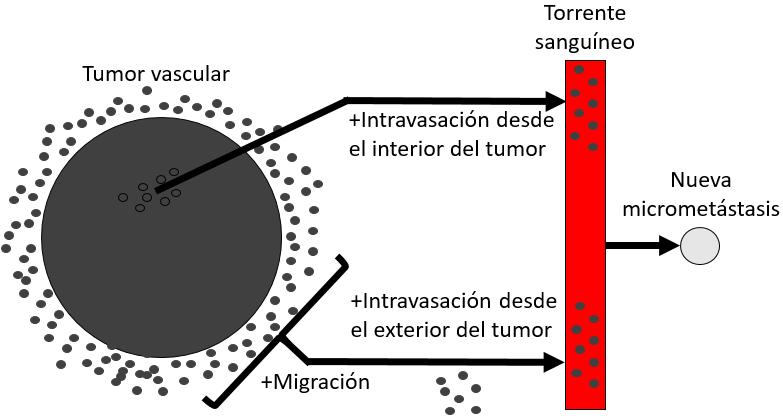
\includegraphics{img/fig-metastasis-vias.png}}
\end{center}\vspace*{-0.6cm}
\caption[Descripci\'on de las distintas rutas de la met\'astasis del c\'ancer]{Descripci\'on de las distintas rutas de la met\'astasis del c\'ancer. Las c\'elulas cancer\'igenas que presentan mutaciones que les permiten migrar a trav\'es de la ECM pueden llevar a cabo la met\'astasis despu\'es de concluir el desplazamiento desde la frontera del tumor hasta un capilar sangu\'ineo presente en los tejidos de sost\'en o desde el interior del propio tumor a trav\'es de los capilares sangu\'ineos que crecen en su interior producto de la angiog\'enesis.}
\label{fig-metastasis-vias}
\end{figure}

Cuando una c\'elula cancer\'igena penetra el sistema circulatorio est\'a expuesta a un n\'umero de peligros que pueden terminar su existencia, entre los que se encuentran principalmente las defensas del sistema inmune que pueden reconocer y destruir estas c\'elulas y el propio estr\'es mec\'anico a que son sometidas producto de su transporte a trav\'es de capilares sangu\'ineos de menor di\'ametro que la propia c\'elula. Eventualmente se adhiere a un posible punto de extravasaci\'on en el que degrada la pared del vaso sangu\'ineo y abandona el sistema circulatorio. Al igual que ocurre con la migraci\'on del c\'ancer, hasta el momento no existe modo de determinar de forma realista la probabilidad de supervivencia de la c\'elula cancer\'igena en su transporte por el sistema circulatorio ni de predecir la localizaci\'on donde dicha c\'elula abandonar\'a el torrente sangu\'ineo, ya que es un fen\'omeno sujeto a muchos procesos de naturaleza aleatoria. Como se expres\'o en la secci\'on~\ref{subsec-meta} la teor\'ia de la semilla y el sustrato es ampliamente aceptada porque permite explicar la tendencia del c\'ancer de colonizar \'organos espec\'ificos. Bas\'andonos en esta teor\'ia se a\~naden un conjunto de hip\'otesis al modelo que permiten representar la met\'astasis del c\'ancer:

\begin{itemize}
\item [XXI.] \textbf{Conexiones distantes del grafo}: \emph{Cada \'organo representado est\'a vinculado con el otro a trav\'es de las conexiones distantes existentes en el grafo subyacente. Se asume que una c\'elula que penetre el sistema circulatorio en un punto dado lo abandonar\'a en una posici\'on predeterminada, correspondientes con los destinos de las conexiones mencionadas.} \label{XXI}
\end{itemize}

La hip\'otesis XXI se apoya en la consideraci\'on que expresa que un tejido vivo puede ser representado mediante una red de mundo peque\~no, planteada en la secci\'on~\ref{subsec-hipo}. El presente modelo reproduce las localizaciones correspondientes con el \'organo donde se origin\'o el tumor y un \'organo que es colonizado de forma preferencial por el tipo de c\'ancer en cuesti\'on, pero es necesario a\~nadir a estas localizaciones una forma que representar las c\'elulas migratorias que permanecen en el interior del sistema circulatorio. La representaci\'on de este transporte a trav\'es del sistema circulatorio debe permitir reproducir la duraci\'on del trayecto y evaluar su supervivencia. 

Supongamos que se tiene una c\'elula que presenta una conexi\'on distante, y como consecuencia de dicha conexi\'on tiene la probabilidad de convertirse en un destino potencial de la met\'astasis. Para representar la migraci\'on se define un conjunto que contiene la informaci\'on correspondiente con todas las c\'elulas migratorias que est\'an viajando a trav\'es del sistema circulatorio con sus destinos. Cuando una c\'elula migratoria alcanza una posici\'on que posee una conexi\'on distante con una c\'elula del estroma que no ha sido colonizada a\'un, la c\'elula migratoria abandona su posici\'on y pasa a pertenecer al conjunto definido anteriormente. Una vez dentro de este conjunto en cada instante de tiempo se prueba su supervivencia hasta que abandone el sistema circulatorio para colonizar finalmente la posici\'on destino. Esta sucesi\'on de pasos describe a grandes rasgos la idea detr\'as de la met\'astasis, pero la posici\'on destino no tiene que ser necesariamente una c\'elula del estroma para que la c\'elula migratoria considere que es un destino viable para la met\'astasis. El destino puede ser una c\'elula del estroma, una c\'elula de un tumor o una c\'elula de una micromet\'astasis. Cada uno de estos destinos se corresponde con las distintas situaciones expuestas en la secci\'on~\ref{subsec-meta} que pueden darse cuando una c\'elula migratoria abandona el sistema circulatorio en una localizaci\'on, de ah\'i que el conjunto que contiene los posibles destinos de la met\'astasis tenga la forma ${\mathcal{E}_{met}}=\lbrace 2,3,5 \rbrace$. Si la c\'elula destino es una c\'elula de un tumor o es alguna micromet\'astasis se infiere que si la c\'elula migratoria sobrevive al transporte y extravasa satisfactoriamente, esta contribuye con la poblaci\'on de dichos tumores. Si la c\'elula destino es una c\'elula del estroma, entonces se crear\'a un nuevo foco cancer\'igeno. No obstante, est\'a fuera del alcance del presente modelo representar estas contribuciones a las poblaciones tumorales. Luego, las c\'elulas migratorias siempre penetran el sistema circulatorio si entran en contacto con una conexi\'on distante, pero solo se almacenan y eval\'uan las que tienen como destino una c\'elula del estroma o una micromet\'astasis, ya que estos tumores pueden ser eliminados por el sistema inmunitario y se debe poder representar la recreaci\'on de estos focos cancerosos. Luego se plantea la siguiente hip\'otesis: 

\begin{itemize}
\item [XXII.] \textbf{Destinos viables de la met\'astasis}: \emph{Se representan solamente las migraciones de c\'elulas cancer\'igenas hacia localizaciones que est\'an sin colonizar o que se corresponden con una micromet\'astasis. Si las localizaciones destino se corresponde con un tumor la c\'elula migratoria abandona su posici\'on y penetra el sistema circulatorio pero no se eval\'ua su transporte ni el arribo a la nueva localizaci\'on.} \label{XXII}
\end{itemize}

Como en el conjunto que representa el sistema circulatorio existen c\'elulas migratorias que poseen una misma posici\'on destino es necesario que sean actualizadas de forma secuencial para manejar las distintas situaciones de competencia, y al igual que sucede con la migraci\'on el orden de actualizaci\'on es aleatorio. La implementaci\'on del los conjunto que representa el sistema circulatorio se logra mediante un conjunto de actualizaci\'on secuencial $C_{sc}^A(G)$ en el que se almacena la informaci\'on referente a las c\'elula migratorias y su destino. Se define un nuevo par\'ametro $\xi_{sc} \in [0,1]$ que es la probabilidad de supervivencia de la c\'elula migratoria en el sistema circulatorio. La incorporaci\'on del conjunto de actualizaci\'on $C_{sc}^A(G)$ y de este par\'ametro al procedimiento de actualizaci\'on se muestra en el algoritmo~\ref{alg-update-3}. El m\'etodo encargado de actualizar las c\'elulas contenidas en el torrente sangu\'ineo se muestra en el algoritmo~\ref{alg-update-3-1}. Como se puede observar en el algoritmo~\ref{alg-update-3}, el transporte en el interior del sistema circulatorio se eval\'ua inicialmente, de forma tal que las c\'elulas que lo penetren como consecuencia de la actualizaci\'on de las c\'elulas migratorias no sean evaluadas hasta el instante de tiempo siguiente.

\begin{algorithm}[!ht]
\caption{Implementaci\'on del procedimiento de actualizaci\'on del aut\'omata celular incorporando el par\'ametro $\xi_{sc}$ y el conjunto de actualizaci\'on secuencial para las c\'elulas migratorias en el interior del sistema circulatorio $C_{sc}^A(G)$.} \label{alg-update-3}
\KwData{$G,\,C_{mig}^A(G),\,C_{sc}^A(G),\,C^S(G),\,S(n),\,\mu_{mig},\,\xi_{sc}$}
$Update$-$Migratory$-$Cells$-$In$-$Bloodstream(C_{sc}^A(G),\,\xi_{sc})$\;
$Update$-$Migratory$-$Cells(G,\,C_{mig}^A(G),\,S(n),\,\mu_{mig})$\;
$Update$-$Synchronous$-$Cells(G,\,C^S(G),S(n))$\;
\end{algorithm}

\begin{algorithm}[!ht]
\caption{Implementaci\'on del m\'etodo $Update$-$Migratory$-$Cells$-$In$-$Bloodstream$ $(C_{sc}^A(G),\xi_{sc})$ utilizado en el procedimiento de actualizaci\'on del aut\'omata celular y que se encarga de la actualizaci\'on del conjunto secuencial que contiene a las c\'elulas migratorias contenidas en el torrente sangu\'ineo.} \label{alg-update-3-1}
\KwData{$C_{sc}^A(G),\,\xi_{sc}$}
\While{$|C_{sc}^A(G)|~\neq~0$}{
	$v=Select$-$Random$-$Vertex(C_{sc}^A(G))$\;
	$w=Get$-$Target$-$Vertex(v,\,C_{sc}^A(G))$\;
	\If{$Random(0,1) \leq \xi_{sc} \wedge s(w,n) = 2$}{		
		$Create$-$New$-$Metastasis(w)$\;}
	$Remove$-$Cell$-$From$-$Bloodstream(v,\,C_{sc}^A(G))$\;}
\end{algorithm}

El algoritmo~\ref{alg-update-3-1} describe el proceso de transporte y extravasaci\'on de las c\'elulas migratorias, luego resta definir el proceso de inserci\'on en el sistema circulatorio. Como se expres\'o anteriormente existen dos posibles situaciones en las que una c\'elula migratoria penetra el torrente sangu\'ineo. Para representar la primera situaci\'on en que la c\'elula migratoria parte desde la frontera del tumor y arriba a un posible punto de intravasaci\'on, se plantea una regla del aut\'omata celular, mientras que para la segunda situaci\'on en la que una c\'elula tumoral provoca el surgimiento de una c\'elula migratoria que penetra directamente el torrente sangu\'ineo, se agregan las instrucciones necesarias al algoritmo~\ref{alg-update-3} en las l\'ineas correspondientes con la actualizaci\'on del conjunto sincronizado $C^S(G)$ para representar dicha situaci\'on. Estas modificaciones consisten en verificar la existencia de una c\'elula tumoral en presencia de una conexi\'on distante, que en caso afirmativo se a\~nade una c\'elula migratoria a la representaci\'on del torrente sangu\'ineo con el destino correspondiente. Una observaci\'on importante es que una misma c\'elula puede poseer m\'as de una conexi\'on distante producto de la aleatoriedad del proceso de reconexi\'on del modelo Watts-Strogatz. Por tanto se sigue el mismo esquema de la regla de la migraci\'on: actualizar el estado de la c\'elula mediante la aplicaci\'on de la regla de la met\'astasis y elegir de forma aleatoria el destino. 

Comenzamos definiendo la regla para la primera situaci\'on descrita anteriormente. Como se expuso en la secci\'on~\ref{subsec-migration} el final de la migraci\'on est\'a dada por la existencia de una conexi\'on distante viable para la met\'astasis en la posici\'on actual de la c\'elula migratoria. Esta condici\'on constituye el criterio de selecci\'on de la regla para la met\'astasis como se muestra a continuaci\'on:
\begin{equation}
s(v,n)=\mathcal{R}(S(v,n))= 2~~\textit{si } s(v,n)=4~\wedge~\mathcal{N}_{\mathcal{E}_{met}}^d(S(v,n))>0. \label{eq-intravasation}
\end{equation}

Se puede apreciar en la expresi\'on~(\ref{eq-intravasation}) que la regla posee un car\'acter determinista, ya que su aplicaci\'on siempre resulta en el abandono de la posici\'on por parte de la c\'elula migratoria. Al aplicarse esta regla la c\'elula migratoria pasa a pertenecer al conjunto de actualizaci\'on secuencial $C_{sc}^A(G)$ con la informaci\'on referente a su destino y con un tiempo de transporte igual a cero. Entonces definimos el proceso de selecci\'on del destino de la met\'astasis como:

\begin{definition}
\label{def-type-neighbours-2}
La funci\'on $D_{met}(v,n)$, que recibe una c\'elula migratoria $v$ y un instante de tiempo $n$, devuelve el conjunto de c\'elulas vecinas distantes de $v$ tales que su estado en el instante de tiempo $n$ est\'e contenido en el conjunto $\mathcal{E}_{met}=\lbrace 2,3,5 \rbrace$, es decir:
\begin{equation}
D_{met}(v,n) = \lbrace w~|~w \in \mathcal{N}^d(v)~\wedge~s(w,n) \in \mathcal{E}_{met} \rbrace. \label{eq-type-neighbours-2}
\end{equation}
\end{definition}

La selecci\'on de la posici\'on destino comienza evaluando la funci\'on~(\ref{eq-type-neighbours-2}) en la c\'elula $v$ en el instante de tiempo actual, obteniendo un conjunto de posibles destinos de la forma $D_{met}(v,n) = \lbrace w_1, w_2, \ldots, w_m \rbrace$ con $m={|D_{met}(v,n)|}$ para luego seleccionar uno de estos de forma aleatoria.

\begin{definition}
\label{def-dest-selection-met}
La funci\'on $d_{met}(v,n)$, que recibe una c\'elula $v$ y un instante de tiempo $n$, devuelve una c\'elula $w$ que pertenece al conjunto $D_{met}(v,n)$ y constituye el destino elegido para la met\'astasis de la c\'elula $v$. El procedimiento queda de la siguiente forma:
\begin{equation}
d_{met}(v,n) = \left\lbrace
	\begin{array}{ll}
		w_1 & \textit{con probabilidad } 1/m\\
		w_2 & \textit{con probabilidad } 1/m\\
		\vdots & \ldots\\
		w_m & \textit{con probabilidad } 1/m
	\end{array}
\right., \label{eq-dest-selection-met}
\end{equation}
donde $D_{met}(v,n)= \lbrace w_1,w_2,\ldots,w_m \rbrace$ con $m = |D_{met}(v,n)|$. Se puede apreciar que todos los destinos viables poseen la misma probabilidad de ser elegidos.
\end{definition}

Finalmente, las modificaciones al algoritmo~\ref{alg-update-3} para representar el surgimiento de una c\'elula migratoria que penetra el sistema circulatorio desde el interior del propio tumor se realizan de forma an\'aloga a las concebidas para representar la migraci\'on, utilizando con este fin un nuevo conjunto de actualizaci\'on sincronizado $C_{tum}^S(G)$ que contiene a las c\'elulas cancer\'igenas que pertenecen al interior de alg\'un tumor vascular y que est\'an en presencia de una conexi\'on distante. El m\'etodo para la actualizaci\'on de estas c\'elulas es el siguiente: por cada c\'elula del conjunto se eval\'ua la probabilidad del surgimiento de una c\'elula descendiente migratoria cuya expresi\'on se expone en~(\ref{eq-migrant-2}) y~(\ref{eq-migrant-3}), y si ocurre la aparici\'on de dicha c\'elula, se coloca en el conjunto de actualizaci\'on secuencial $C_{sc}^A(G)$ con su destino seleccionado de forma aleatoria de entre los posibles. La necesidad de incluir este mecanismo para el surgimiento de c\'elulas migratorias est\'a dada por la representaci\'on del sistema circulatorio, impidiendo que pueda representarse propiamente mediante una regla del aut\'omata. El procedimiento de actualizaci\'on incorporando el nuevo conjunto de actualizaci\'on y el m\'etodo correspondiente se muestran en los algoritmos~\ref{alg-update-4} y~\ref{alg-update-4-1} respectivamente. 

\begin{algorithm}[!ht]
\caption{Implementaci\'on del procedimiento de actualizaci\'on del aut\'omata celular incorporando el conjunto de actualizaci\'on sincronizado para las c\'elulas migratorias que penetran el sistema circulatorio desde una conexi\'on distante en el interior de un tumor $C_{tum}^S(G)$.} \label{alg-update-4}
\KwData{$G,\,C_{mig}^A(G),\,C_{sc}^A(G),\,C_{tum}^S(G),\,C^S(G),\,S(n),\,\mu_{mig},\,\xi_{sc},\,N_{tum},\,n$}
$Update$-$Migratory$-$Cells$-$In$-$Bloodstream(C_{sc}^A(G),\,\xi_{sc})$\;
$Update$-$Migratory$-$Cells(G,\,C_{mig}^A(G),S(n),\,\mu_{mig})$\;
$Update$-$Tumor$-$Migratory$-$Cells(G,\,C_{tum}^S(G),\,C_{sc}^A(G),\,S(n),\,N_{tum},\,n)$\;
$Update$-$Synchronous$-$Cells(G,\,C^S(G),S(n))$\;
\end{algorithm}

\begin{algorithm}[!ht]
\caption{Implementaci\'on del m\'etodo $Update$-$Tumor$-$Migratory$-$Cells(G,S(n),$  $C_{tum}^S(G),C_{sc}^A(G),\,N_{tum},\,n)$ utilizado en el procedimiento de actualizaci\'on del aut\'omata celular y que se encarga de la actualizaci\'on del conjunto sincronizado que contiene a las c\'elulas tumorales que est\'an en presencia de una conexi\'on distante y cuya descendencia migratoria posee la probabilidad de intravasar al interior del sistema circulatorio.} \label{alg-update-4-1}
\KwData{$G,\,S(n),\,C_{tum}^S(G),\,C_{sc}^A(G),\,N_{tum},\,n$}
\For{$v \in C_{tum}^S(G)$}{
	$p=Get$-$Probability(n - N_{tum}[tumor(v)])$\;
	\If{$Random(0,1) \leq p$}{
		$d=Select$-$Destiny$-$Vertex(v,\,S(n),\,G)$\;
		$Add$-$Cell$-$To$-$Bloodstream(v,\,d,\,C_{sc}^A(G))$\;}}
\end{algorithm}

\subsection{Reglas del crecimiento de una micromet\'astasis}
\label{subsec-micrometastasis}
En la secci\'on~\ref{subsec-celldiv} se expuso una caracterizaci\'on de los distintos tipos de tumores que se presentan en el modelo, que concluy\'o con la definici\'on de la regla para el crecimiento de los tumores primarios y de los secundarios durante la etapa vascular. En la presente secci\'on se definen el conjunto de reglas que determinan el crecimiento de las micromet\'astasis, es decir, los tumores secundarios en etapa avascular. En la caracterizaci\'on antes mencionada se describieron las micromet\'astasis como conjuntos formados por c\'elulas que culminaron el proceso de acumulaci\'on de mutaciones por lo que comienzan a desarrollar la angiog\'enesis desde un primer momento y como consecuencia pueden expandirse hacia todos los tejidos sanos. No obstante, durante esta etapa de su desarrollo son vulnerables ya que la colonizaci\'on satisfactoria est\'a sujeta a dos factores vitales en los que se apoya la teor\'ia de la semilla y el sustrato expuesta en la secci\'on~\ref{subsec-meta}. El nuevo entorno de crecimiento puede ser muy diferente a la localizaci\'on donde el c\'ancer se origin\'o y puede ser capaz o no de responder a los intentos de las c\'elulas cancer\'igenas de modificarlo para asegurar su proliferaci\'on. Una micromet\'astasis puede permanecer largos per\'iodos de tiempo en esta forma, siendo capaz de crecer solamente hasta la poblaci\'on permitida por la difusi\'on de nutrientes y es solo cuando logra promover la suficiente angiog\'enesis que cambia su condici\'on de micromet\'astasis a la de un tumor en etapa vascular. Este per\'iodo de tiempo se conoce como dormancia o latencia y el mecanismo que lo reproduce se explicar\'a en la secci\'on~\ref{subsec-dormancy} que aparece posteriormente. El procedimiento propuesto es similar al mostrado en la secci\'on~\ref{subsec-celldiv} referente al crecimiento de tumores, y adopta la hip\'otesis XVII sobre el sesgo direccional del crecimiento tumoral basada en la variaci\'on de la concentraci\'on de nutrientes, mientras que redefine la hip\'otesis XV sobre la competencia entre tumores por expandirse a una posici\'on para adaptarla a las competencias entre micromet\'astasis.

\begin{itemize}
\item [{XXIII.}] \textbf{Situaciones de competencia entre micromet\'astasis}: \emph{En las situaciones de competencia de varias micromet\'astasis por expandirse a una misma posici\'on se asume que el valor de la probabilidad de transici\'on se corresponde con la micromet\'astasis con mayor probabilidad de expansi\'on en ese momento.} \label{XXIII}
\end{itemize}

Se plantea una extensi\'on de la probabilidad de transici\'on expuesta en~\ref{def-local-func} de forma que reciba los argumentos requeridos en la definici\'on de la regla an\'aloga a la mostrada en~\ref{prop-newlocal-func-2-1}. 

\begin{definition}
\label{prop-newlocal-func-5}
Sea una extensi\'on de la funci\'on de transici\'on local definida en~\ref{def-local-func} que incluye una probabilidad de transici\'on alternativa que depende de nuevos argumentos:
\begin{equation}
s(v,n+1) = \mathcal{R}(S(v,n)) = e_i~~\textit{con probabilidad } \rho(v,\tau(v,n,N_{mic},L_{mic}) \rightarrow e_i), \label{eq-newlocal-func-5}
\end{equation}
donde $\tau(v,n,N_{mic},L_{mic})$ es una funci\'on que devuelve un conjunto compuesto por tuplas correspondientes con cada micromet\'astasis que intenta expandirse hacia $v$ en el instante de tiempo $n$ que contienen el tiempo transcurrido relativo al surgimiento de dicha micromet\'astasis y el conjunto de c\'elulas que lo conforman. 
\end{definition}

El conjunto $N_{mic}$ contiene la informaci\'on correspondiente con los instantes de tiempo en que surgieron las micromet\'astasis contenidas en la simulaci\'on. El conjunto $L_{mic}$ contiene la informaci\'on correspondiente con los conjuntos de c\'elulas que conforman las micromet\'astasis contenidas en la simulaci\'on. La funci\'on $\tau(v,n,N_{mic},L_{mic})$ se define de forma an\'aloga a la funci\'on $\tau(v,n,N_{tum},L_{tum})$. En el algoritmo~\ref{alg-L-c-1} se muestra la implementaci\'on de la funci\'on $\tau(v,n,N_{mic},L_{mic})$ a modo de definici\'on donde $N^n(v)$ es la funci\'on de vecindad inmediata definida en~\ref{def-neighbourhoods}, la funci\'on $tumor(w)$ devuelve el identificador \'unico asociado a la micromet\'astasis a la que pertenece $w$ y la funci\'on $s(w,n)$ es el estado de la c\'elula $w$ en el instante de tiempo $n$ definida en~\ref{def-cellstatus}. 

\begin{algorithm}[!ht]
\caption{Definici\'on de la funci\'on $\tau(v,n,N_{mic},L_{mic})$.} \label{alg-L-c-1}
\KwData{$v, n, N_{mic}, L_{mic}$}
\KwResult{$L$}
$L = \lbrace \rbrace$\;
\For{$w \in N^n(v)$}{
	\If{$s(w,n)=5$}{
		$l = L_{mic}[tumor(w)]$\;
		$n_r = n - N_{mic}[tumor(w)]$\;
		$L = L \cup \lbrace \langle n_r, l \rangle \rbrace$\;}}
\Return $L$\;
\end{algorithm}

Se define el conjunto de reglas para el crecimiento de las micromet\'astasis tomando en cuenta la nueva probabilidad de transici\'on alternativa~(\ref{eq-newlocal-func-5}) como:
\begin{equation}
s(v,n+1)=\mathcal{R}(S(v,n))=\left\lbrace
	\begin{array}{ll}
		\zeta_{50}(v,\tau(v,n,N_{mic},L_{mic}))& \textit{si } s(v,n)=0~\wedge~\mathcal{N}_5^n(S(v,n)) > 0~\wedge\\
								       & \mathcal{N}_3^n(S(v,n))=0 \\
		\zeta_{51}(v,\tau(v,n,N_{mic},L_{mic}))& \textit{si } s(v,n)=1~\wedge~\mathcal{N}_5^n(S(v,n)) > 0~\wedge\\
								       & \mathcal{N}_3^n(S(v,n))=0 \\
		\zeta_{52}(v,\tau(v,n,N_{mic},L_{mic}))& \textit{si } s(v,n)=2~\wedge~\mathcal{N}_5^n(S(v,n)) > 0~\wedge\\
								       & \mathcal{N}_3^n(S(v,n))=0  
	\end{array}
\right., \label{eq-celldiv-5}
\end{equation}
donde la distribuci\'on de probabilidad de las variables aleatorias $\zeta_{50}(v,\tau(v,n,N_{mic},L_{mic}))$, $\zeta_{51}$ $(v,\tau(v,n,N_{mic},L_{mic}))$ y $\zeta_{52}(v,\tau(v,n,N_{mic},L_{mic}))$ quedar\'ian como:
\begin{subequations}
\begin{multline}
P(\zeta_{50}(v,\tau(v,n,N_{mic},L_{mic}))=0) = P(\zeta_{51}(v,\tau(v,n,N_{mic},L_{mic}))=1) = \\P(\zeta_{52}(v,\tau(v,n,N_{mic},L_{mic}))=2) = 1 - \rho_5(v,\tau(v,n,N_{mic},L_{mic}) \rightarrow 5),
\end{multline}
\begin{multline}
P(\zeta_{50}(v,\tau(v,n,N_{mic},L_{mic}))=5) = P(\zeta_{51}(v,\tau(v,n,N_{mic},L_{mic}))=5) = \\P(\zeta_{52}(v,\tau(v,n,N_{mic},L_{mic}))=5) = \rho_5(v,\tau(v,n,N_{mic},L_{mic}) \rightarrow 5).
\end{multline}
\end{subequations}

De las expresiones anteriores se infiere que la probabilidad de que una c\'elula normal sea desplazada por una c\'elula cancer\'igena perteneciente a una micromet\'astasis tiene el valor correspondiente con la evaluaci\'on de la probabilidad de transici\'on $\rho_5(v,\tau(v,n,N_{mic},L_{mic}) \rightarrow 5)$, mientras que la probabilidad de que permanezca en el estado original es $1-\rho_5(v,\tau(v,n,N_{mic},L_{mic}) \rightarrow 5)$. Estas reglas reproducen la expansi\'on de la micromet\'astasis hacia los distintos tipos de tejidos sanos que se representan en el aut\'omata, que como se puede observar, poseen las mismas probabilidades independientemente del tipo de tejido. Los criterios de selecci\'on se definen utilizando la funci\'on $\mathcal{N}_{\mathcal{E'}}^n(S(v,n))$ planteada en~\ref{def-near-neighbours} y representan la situaci\'on donde la c\'elula $v$ posee en su vecindad inmediata c\'elulas pertenecientes a una o varias micromet\'astasis mediante la condici\'on $\mathcal{N}_5^n(S(v,n)) > 0$. Siguiendo las interpretaciones biol\'ogicas de las hip\'otesis XVII y XXIII sobre el sesgo direccional del crecimiento tumoral y las situaciones de competencia entre micromet\'astasis respectivamente, una micromet\'astasis no deber\'ia expandirse hacia un tumor de mayor desarrollo que obtiene la mayor\'ia de los nutrientes del entorno, por lo que se a\~nade la condici\'on $\mathcal{N}_3^n(S(v,n))=0$ a las reglas. De esta forma la selecci\'on de las reglas para el crecimiento tumoral y para el crecimiento de las micromet\'astasis puede hacerse de forma inequ\'ivoca y priorizando a los tumores en etapa vascular. Seg\'un la hip\'otesis XXIII la expresi\'on para el c\'alculo de la probabilidad de transici\'on $\rho_5(v,\tau(v,n,N_{mic},L_{mic}) \rightarrow 5)$ quedar\'ia como:
\begin{equation}
\rho_5(v,\tau(v,n,N_{mic},L_{mic}) \rightarrow 5) = max[\rho_5(v,n_1,l_1 \rightarrow 5),\rho_5(v,n_2,l_2 \rightarrow 5),\ldots, \rho_5(v,n_m,l_m \rightarrow 5)], 
\end{equation}
donde $n_i$ y $l_i$ son los valores de la tupla $\langle n_i, l_i \rangle \in \tau(v,n,N_{mic},L_{mic})$ con $i \in \lbrace 1,2,\ldots,m \rbrace$ y $m=|\tau(v,n,N_{mic},L_{mic})|$ correspondiente con la i-\'esima micromet\'astasis que se intenta expandir hacia $v$. La probabilidad espec\'ifica a cada una de estas micromet\'astasis se plantea utilizando la probabilidad general del crecimiento tumoral~(\ref{eq-generaldivrule}), las hip\'otesis XVII y XVIII sobre el sesgo direccional y la velocidad de expansi\'on tumoral, y las funciones $\beta_{tum}(v,l)$ y $\gamma_{tum}(v,N(v,l))$ definidas en~\ref{def-beta} y~\ref{def-velocity-function} como:
\begin{equation}
\rho_5(v,n_i,l_i \rightarrow 5) = \left\lbrace
	\begin{array}{ll}
		\gamma_{tum}(v,N(v,l_i))\,\beta_{tum}(v,l_i)\,\rho_a(n_i \Delta t)& \textit{si } n_i \leq n_a \\
		0& \textit{si } n_i > n_a
	\end{array}
\right.. \label{eq-rho-5}
\end{equation}

Si se escribe en t\'erminos de la funci\'on tipo Heaviside definida en~\ref{def-heaviside} la expresi\'on anterior quedar\'ia como:
\begin{equation}
\rho_5(v,n_i,l_i \rightarrow 5) = H(n) \gamma_{tum}(v,N(v,l_i)) \beta_{tum}(v,l_i) \rho_a(n_i \Delta t). \label{eq-rho-51}
\end{equation}

De la expresiones~(\ref{eq-rho-5}) y~(\ref{eq-rho-51}) se infiere que una micromet\'astasis no crece m\'as all\'a de la poblaci\'on m\'axima permitida por la difusi\'on de nutrientes. En la secci\'on~\ref{subsec-dormancy} que aparece a continuaci\'on se define el mecanismo para representar la dormancia de una micromet\'astasis y de c\'omo abandona esa condici\'on para convertirse en un tumor en etapa vascular.

\subsection{Reglas de la dormancia de una micromet\'astasis}
\label{subsec-dormancy}
Una micromet\'astasis se forma cuando una o varias c\'elulas emergen del sistema circulatorio en un punto de extravasaci\'on y proceden a colonizar esa localizaci\'on. La teor\'ia de la semilla y el sustrato estipula que la nueva localizaci\'on puede ser muy distinta al entorno donde se origin\'o el c\'ancer obstaculizando su progresi\'on. Dependiendo del \'organo destino pueden darse tres situaciones distintas. En primer lugar, el entorno puede ser similar con el tejido donde se origin\'o el c\'ancer, en el mejor de los escenarios se corresponde con el mismo \'organo original. En este caso el per\'iodo de dormancia termina relativamente r\'apido. La segunda situaci\'on se corresponde con un entorno medianamente hostil donde la dormancia se extiende durante un per\'iodo de tiempo prolongado, hasta que la micromet\'astasis culmine el proceso de colonizaci\'on. El tercer caso se corresponde con los \'organos donde una micromet\'astasis no puede sobrevivir porque posee profundas diferencias con el entorno donde se origin\'o. En el presente modelo solo se reproducen las primeras dos situaciones ya que el \'organo secundario constituye un destino preferencial de la met\'astasis, hecho por el que se asume que posee un entorno similar o medianamente hostil comparado con el \'organo primario. Adem\'as, como se plante\'o en las secciones~\ref{subsec-meta} y~\ref{subsec-micrometastasis} durante la colonizaci\'on una micromet\'astasis est\'a en constante peligro de ser eliminada por el sistema inmunitario independientemente del \'organo donde est\'e localizada.

Del an\'alisis anterior se infiere que el desarrollo de una micromet\'astasis est\'a sujeta a dos posibles par\'ametros del modelo: una probabilidad de supervivencia $\xi_{mic} \in [0,1]$ y una probabilidad de colonizaci\'on $\psi_{mic} \in [0,1]$. En cada instante de tiempo se determina la supervivencia de la micromet\'astasis en base al par\'ametro $\xi_{mic}$ y si su supervivencia es evaluada como positiva se determina si la micromet\'astasis puede abandonar la dormancia y convertirse en un tumor que coloniz\'o satisfactoriamente la localizaci\'on y no est\'a sujeto a la probabilidad de supervivencia. Finalmente se reproduce su crecimiento mediante la regla declarada en la secci\'on~\ref{subsec-micrometastasis}. La representaci\'on del proceso descrito se logra mediante la inclusi\'on de los par\'ametros $\xi_{mic0}$, $\psi_{mic0}$, $\xi_{mic1}$ y $\psi_{mic1}$ correspondientes con cada localizaci\'on del tejido representado al procedimiento de actualizaci\'on del aut\'omata celular mediante la adici\'on de dos nuevos m\'etodos que se encargan de probar la supervivencia de la micromet\'astasis as\'i como su colonizaci\'on satisfactoria y posterior conversi\'on a un tumor secundario, como se muestra en los algoritmos~\ref{alg-update-5},~\ref{alg-update-5-1} y~\ref{alg-update-5-2}. Las c\'elulas que conforman la micromet\'astasis fallida o exitosa son actualizadas mediante el uso de la regla que se define a continuaci\'on. Se plantea una extensi\'on de la probabilidad de transici\'on expuesta en~\ref{def-local-func} de forma que reciba los argumentos requeridos en la definici\'on de la regla para la actualizaci\'on de las c\'elulas pertenecientes a una micromet\'astasis. 

\begin{algorithm}[!ht]
\caption{Implementaci\'on del procedimiento de actualizaci\'on del aut\'omata celular incorporando los par\'ametros $\xi_{mic0}$, $\psi_{mic0}$, $\xi_{mic0}$ y $\psi_{mic0}$ y los conjuntos $L_{mic}$ y $N_{mic}$.} \label{alg-update-5}
\KwData{$C_{mig}^A(G),\,C_{sc}^A(G),\,C_{tum}^S(G),\,C^S(G),\,S(n),\,\mu_{mig},\,\xi_{sc},\,\xi_{mic0},\,$ $\psi_{mic0},\,\xi_{mic1},\,$ $\psi_{mic1},\,N_{tum},\,L_{mic},\,N_{mic},\,n$}
$Update$-$Migratory$-$Cells$-$In$-$Bloodstream(C_{sc}^A(G),\,\xi_{sc})$\;
$Update$-$Migratory$-$Cells(G,\,C_{mig}^A(G),S(n),\,\mu_{mig})$\;
$Update$-$Tumor$-$Migratory$-$Cells(G,\,S(n),\,C_{tum}^S(G),\,C_{sc}^A(G),\,N_{tum},\,n)$\;
$Check$-$Micrometastasis$-$Survival(L_{mic},\,S(n),\,\xi_{mic0},\,\xi_{mic1})$\;
$Check$-$Micrometastasis$-$Colonization(L_{mic},\,N_{mic},\,S(n),\,\psi_{mic0},\,\psi_{mic1},\,n)$\;
$Update$-$Synchronous$-$Cells(G,\,C^S(G),S(n))$\;
\end{algorithm}

\begin{algorithm}[!ht]
\caption{Implementaci\'on del m\'etodo $Check$-$Micrometastasis$-$Survival(L_{mic},$ $S(n),\,\xi_{mic0},\,\xi_{mic1})$ utilizado en el procedimiento de actualizaci\'on del aut\'omata celular y que verifica la supervivencia de las micromet\'astasis en el nuevo entorno a colonizar.} \label{alg-update-5-1}
\KwData{$L_{mic},\,S(n),\,\xi_{mic0},\,\xi_{mic1}$}
\For{$l \in L_{mic}$}{
	$\xi = Get$-$Organ$-$Probabilities(l, \xi_{mic0}, \xi_{mic1})$\;
	$r = Random(0,1)$\;
	\For{$v \in l$}{
		$Apply$-$Local$-$Transition$-$Function$-$Met$-$Sur(v,\,S(n),\,G,\,r,\,\xi)$\;}}
\end{algorithm}

\begin{algorithm}[!ht]
\caption{Implementaci\'on del m\'etodo $Check$-$Micrometastasis$-$Colonization(L_{mic},$ $N_{mic},\,S(n),\,\psi_{mic0},\,\psi_{mic1},\,n)$ utilizado en el procedimiento de actualizaci\'on del aut\'omata celular y que verifica la colonizaci\'on satisfactoria del entorno por parte de las micromet\'astasis.} \label{alg-update-5-2}
\KwData{$L_{mic},\,N_{mic},\,S(n),\,\psi_{mic0},\,\psi_{mic1},\,n$}
\For{$l \in L_{mic}$}{
	$\psi = Get$-$Organ$-$Probabilities(l, \psi_{mic0}, \psi_{mic1})$\;
	$n_r = n - N_{mic}[tumor(l)]$\;
	$r = Random(0,1)$\;
	\For{$v \in l$}{		
		$Apply$-$Local$-$Transition$-$Function$-$Met$-$Col(v,\,S(n),\,G,\,r,\,n_r,\,\psi)$\;}}
\end{algorithm} 

\begin{definition}
\label{prop-newlocal-func-6}
Sea una extensi\'on de la funci\'on de transici\'on local definida en~\ref{def-local-func} que incluye una probabilidad de transici\'on alternativa que depende de nuevos argumentos:
\begin{equation}
s(v,n) = \mathcal{R}(S(v,n)) = e_i~~\textit{con probabilidad } \rho(n_r,r \rightarrow e_i), \label{eq-newlocal-func-6}
\end{equation}
donde $n_r$ es un valor entero y $r$ es un valor real.
\end{definition}

Se define el conjunto de reglas para la actualizaci\'on de las c\'elulas pertenecientes a una micromet\'astasis tomando en cuenta la nueva probabilidad de transici\'on alternativa~(\ref{eq-newlocal-func-6}) como:
\begin{equation}
s(v,n)=\mathcal{R}(S(v,n))=\zeta_{5}(n_r,r)~~\textit{si } s(v,n)=5, \label{eq-celldiv-6}
\end{equation}
donde la distribuci\'on de probabilidad de la variable aleatoria $\zeta_{5}(n_r,r) \in \lbrace 2,3,5 \rbrace$ es:
\begin{subequations}
\begin{equation}
P(\zeta_{5}(n_r,r)=2) = \rho_5(n_r,r \rightarrow 2),
\end{equation}
\begin{equation}
P(\zeta_{5}(n_r,r)=3) = \rho_5(n_r,r \rightarrow 3),
\end{equation}
\begin{equation}
P(\zeta_{5}(n_r,r)=5) = 1 - max[\rho_5(n_r,r \rightarrow 2),\rho_5(n_r,r \rightarrow 3)].
\end{equation}
\end{subequations}

Las probabilidades de transici\'on $\rho_5(n_r,r \rightarrow 2)$ y $\rho_5(n_r,r \rightarrow 3)$ deciden en base a los par\'ametros pasados como argumentos de las funciones $Apply$-$Local$-$Transition$-$Function$-$Met$-$Sur$ y $Apply$-$Local$-$Transition$-$Function$-$Met$-$Col$ si una micromet\'astasis se transforma satisfactoriamente en un tumor o es eliminada de la simulaci\'on, quedando como:
\begin{subequations}
\begin{equation}
\rho_5(n_r,r \rightarrow 2) = \left\lbrace
	\begin{array}{ll}
		1& \textit{si } r \leq 1 - \xi \\
		0& \textit{si } r > 1 - \xi
	\end{array}
\right., \label{eq-rho-5-sur}
\end{equation}
\begin{equation}
\rho_5(n_r,r \rightarrow 3) = \left\lbrace
	\begin{array}{ll}
		1& \textit{si } n_r \geq n_a \wedge r \leq \psi \\
		0& \textit{si } n_r < n_a
	\end{array}
\right.. \label{eq-rho-5-col}
\end{equation}
\end{subequations}

Como se puede apreciar en las expresiones~\ref{eq-rho-5-sur} y~\ref{eq-rho-5-col} los valores de $n_r$, $r$, $\xi$ y $\psi$ son los mismos para todas las c\'elulas de una misma micromet\'astasis ya que se determinan a priori en los algoritmos de actualizaci\'on correspondientes, logrando que todas cambien al mismo estado final. Habiendo culminado el proceso de concepci\'on del conjunto de reglas, en la secci\'on~\ref{sec-validation} se exponen los procedimientos que se llevan a cabo para determinar los par\'ametros del modelo de aut\'omatas celulares que se presenta en este manuscrito. 


%\newpage
%\subsection{Resumen de la din\'amica del aut\'omata celular}
\label{subsec-resumen}
En las secciones~\ref{subsec-celldiv}, \ref{subsec-migrant}, \ref{subsec-migration}, \ref{subsec-metastasis}, \ref{subsec-micrometastasis} y \ref{subsec-dormancy} se expuso el proceso gradual de concepci\'on de la din\'amica del aut\'omata celular, basada en dos componentes fundamentales: el conjunto de reglas y en el procedimiento de actualizaci\'on. Como el t\'itulo de esta secci\'on lo indica se presenta una recapitulaci\'on final de estos componentes fundamentales antes de pasar a las tareas de an\'alisis de resultados y validaci\'on del modelo. 

\subsubsection{Procedimiento de actualizaci\'on}
Dada la naturaleza de las distintas entidades biol\'ogicas que se recogen en el presente modelo de aut\'omatas celulares, presentadas en la secci\'on~\ref{subsec-states}, no es posible implementar el procedimiento cl\'asico de actualizaci\'on s\'incrona en el que se aplica la funci\'on de transici\'on local a todas las c\'elulas del aut\'omata de forma simult\'anea. Como se expuso a lo largo de la secci\'on~\ref{subsec-migration} se adopta un enfoque h\'ibrido en el que cada tipo de c\'elula es tratada seg\'un su propia naturaleza y las reglas del aut\'omata que rigen su comportamiento. En el cuadro~\ref{table-update-set} se muestran los conjuntos de actualizaci\'on definidos mostrando los tipos de c\'elulas contenidas en los mismos y el modo en que se llevan a cabo, es decir, de forma s\'incrona o as\'incrona. En adici\'on a estos conjuntos se definen un n\'umero de par\'ametros que cumplen un papel fundamental en el procedimiento de actualizaci\'on, como se muestra en el cuadro~\ref{table-update-params}. Finalmente el procedimiento de actualizaci\'on y cada uno de los m\'etodos que lo componen se muestran en los algoritmos~\ref{alg-update-r}, \ref{alg-update-r-1}, \ref{alg-update-r-2}, \ref{alg-update-r-3}, \ref{alg-update-r-4}, \ref{alg-update-r-5} y \ref{alg-update-r-6} respectivamente. Para m\'as informaci\'on verifique las reglas del aut\'omata celular presentadas posteriormente.

\begin{table}[h!]
\begin{center}
\scalebox{0.9}{\begin{tabular}{|p{2cm}|p{14.5cm}|} \hline
\emph{Par\'ametro} & \emph{Descripci\'on} \\\hline
\multicolumn{1}{|c|}{$C^S(G)$} & Conjunto de actualizci\'on s\'incrono. Contiene a las c\'elulas normales correspondientes con el lumen (estado $0$), el epitelio (estado $1$) y el estroma (estado $2$), as\'i como a las c\'elulas tumorales (estado $3$) que no poseen conexiones distantes y las c\'elulas de las micromet\'astasis (estado $5$). \\\hline
\multicolumn{1}{|c|}{$C_{mig}^A(G)$} & Conjunto de actualizaci\'on as\'incrono. Contiene a las c\'elulas migratorias del c\'ancer (estado $4$). \\\hline
\multicolumn{1}{|c|}{$C_{sc}^A(G)$} & Conjunto de actualizaci\'on as\'incrono. Contiene a las c\'elulas migratorias del c\'ancer que residen en el sistema circulatorio. \\\hline
\multicolumn{1}{|c|}{$C_{tum}^S(G)$} & Conjunto de actualizaci\'on s\'incrono. Contiene a las c\'elulas tumorales (estado $3$) que poseen conexiones distantes. \\\hline
\end{tabular}}\vspace*{-0.5cm}
\end{center}
\caption[Resumen de los conjuntos utilizados en el procedimiento de actualizaci\'on]{Resumen de los conjuntos utilizados en el procedimiento de actualizaci\'on.}
\label{table-update-set}
\end{table}

\begin{table}[h!]
\begin{center}
\scalebox{0.9}{\begin{tabular}{|p{2cm}|p{14.5cm}|} \hline
\emph{Par\'ametro} & \emph{Descripci\'on} \\\hline
\multicolumn{1}{|c|}{$\psi_{mig}$} & Probabilidad de la c\'elula migratoria de llevar a cabo un desplazamiento. \\\hline
\multicolumn{1}{|c|}{$\mu_{mig}$} & Cantidad de movimientos tentativos que la c\'elula migratoria puede llevar a cabo en un instante de tiempo.\\\hline
\multicolumn{1}{|c|}{$\xi_{sc}$} & Probabilidad de supervivencia de una c\'elula migratoria durante el transporte en el sistema circulatorio.\\\hline
\multicolumn{1}{|c|}{$\psi_{met0}$, $\psi_{met1}$} & Probabilidad de la c\'elula migratoria de arribar al \'organo destino correspondiente. \\\hline
\multicolumn{1}{|c|}{$\xi_{mic}$} & Probabilidad de supervivencia de una micromet\'astasis.\\\hline
\multicolumn{1}{|c|}{$\psi_{mic}$} & Probabilidad de colonizaci\'on de una micromet\'astasis.\\\hline
\end{tabular}}\vspace*{-0.5cm}
\end{center}
\caption[Resumen de los par\'ametros del procedimiento de actualizaci\'on]{Resumen de los par\'ametros del procedimiento de actualizaci\'on.}
\label{table-update-params}
\end{table}

\begin{algorithm}[h!]
\caption{Implementaci\'on del procedimiento de actualizaci\'on del aut\'omata celular.} \label{alg-update-r}
\KwData{$C_{mig}^A(G),\,C_{sc}^A(G),\,C_{tum}^S(G),\,C^S(G),\,S(n),\,\psi_{mig},\,\mu_{mig},\,\xi_{sc},\,\psi_{met0},\,\psi_{met1},\,\xi_{mic},\,$ $\psi_{mic},\,L_{mic}(n)$}
$update-migratory-cells-in-bloodstream(C_{sc}^A(G),\,\psi_{met0},\,\psi_{met1},\,\xi_{sc})$\;
$update-migratory-cells(G,\,C_{mig}^A(G),S(n),\,\psi_{mig},\,\mu_{mig})$\;
$update-tumor-migratory-cells(G,\,C_{tum}^S(G),\,C_{sc}^A(G),\,S(n))$\;
$check-micrometastasis-survival(L_{mic}(n),\,S(n),\,\xi_{mic})$\;
$update-synchronous-cells(G,\,C_{sc}^A(G),\,C^S(G),\,S(n))$\;
$check-micrometastasis-colonization(L_{mic}(n),\,S(n),\,\psi_{mic})$\;
\end{algorithm}

\begin{algorithm}[h!]
\caption{Implementaci\'on del m\'etodo $update-migratory-cells-in-bloodstream$ $(C_{sc}^A(G),\,\psi_{met0},\,\psi_{met1},\,\xi_{sc})$ encargado de la actualizaci\'on del conjunto as\'incrono que contiene a las c\'elulas migratorias contenidas en el torrente sangu\'ineo.} \label{alg-update-r-1}
\KwData{$C_{sc}^A(G),\,\xi_{sc},\,\psi_{met0},\,\psi_{met1}$}
\While{$|C_{sc}^A(G)|~\neq~0$}{
	$v=select-random-vertex(C_{sc}^A(G))$\;
	$w=get-target-vertex(v,\,C_{sc}^A(G))$\;
	$\psi=get-target-organ-probability(w,\,\psi_{met0},\,\psi_{met1})$\;
	\If{$random(0,1) \leq \xi_{sc} \wedge random(0,1) \leq \psi \wedge s(w,n) = 2$}{		
		$create-new-metastasis(w)$\;}
	$remove-cell-from-bloodstream(v,\,C_{sc}^A(G))$\;}
\end{algorithm}

\begin{algorithm}[p]
\caption{Implementaci\'on del m\'etodo $update-migratory-cells(G,\,C_{mig}^A(G),\,S(n),$ $\psi_{mig},\,\mu_{mig})$ encargado de la actualizaci\'on del conjunto as\'incrono que contiene a las c\'elulas migratorias.} \label{alg-update-r-2}
\KwData{$G,\,C_{mig}^A(G),\,S(n),\,\psi_{mig},\,\mu_{mig}$}
$updated=\lbrace \rbrace$\;
$i=0$\;
\While{$i < \mu_{mig}$}{
	\While{$|C_{mig}^A(G)|~\neq~|updated|$}{
		\Repeat{$v \notin updated$}{
			$v=select-random-vertex(C_{mig}^A(G))$\;}
		\If{$random(0,1) \leq \psi_{mig}$}{
			$apply-local-transition-function(v,\,S(n),\,G)$\;}
		$updated = updated \cup v$\;}
	$updated=\lbrace \rbrace$\;	
	$i++$\;}
\end{algorithm}

\begin{algorithm}[p]
\caption{Implementaci\'on del m\'etodo $update-tumor-migratory-cells(G,\,$ $C_{tum}^S(G),\,C_{sc}^A(G),\,S(n))$ encargado de la actualizaci\'on del conjunto as\'incrono que contiene a las c\'elulas tumorales que est\'an en presencia de una conexi\'on distante y cuya descendencia migratoria tiene la posibilidad de penetrar el sistema circulatorio.} \label{alg-update-r-3}
\KwData{$G,\,C_{tum}^S(G),\,C_{sc}^A(G),\,S(n)$}
\For{$v \in C_{tum}^S(G)$}{
	$p=get-probability(v)$\;
	\If{$random(0,1) \leq p$}{
		$d=select-destiny-vertex(v,\,S(n),\,G)$\;
		$add-cell-to-bloodstream(v,\,d,\,C_{sc}^A(G))$\;}}
\end{algorithm}

\begin{algorithm}[p]
\caption{Implementaci\'on del m\'etodo $check-micrometastasis-survival(L_{mic}(n),\,$ $S(n),\,\xi_{mic})$ encargado de verificar la supervivencia de las micromet\'astasis en el nuevo entorno a colonizar.} \label{alg-update-r-4}
\KwData{$L_{mic}(n),\,S(n),\,\xi_{mic}$}
\For{$l \in L_{mic}(n)$}{
	\If{$random(0,1) \leq 1 - \xi_{mic}$}{
		\For{$v \in l$}{
			$set-cell-status(S(n),\,v,\,2)$\;}}}
\end{algorithm}

\begin{algorithm}[h!]
\caption{Implementaci\'on del m\'etodo $update-synchronous-cells(G,\,C^S(G),\,S(n))$ encargado de la actualizaci\'on del conjunto s\'incrono que contiene a las c\'elulas normales, tumorales y las pertenecientes a las micromet\'astasis.} \label{alg-update-r-5}
\KwData{$G,\,C^S(G),\,S(n)$}
\For{$v \in C^S(G)$}{
	$apply-local-transition-function(v,\,S(n),\,G)$\;}
\end{algorithm}

\begin{algorithm}[h!]
\caption{Implementaci\'on del m\'etodo $check-micrometastasis-colonization$ $(L_{mic}(n),\,S(n),\,\psi_{mic})$ encargado de verificar la colonizaci\'on satisfactoria del entorno por parte de las micromet\'astasis.} \label{alg-update-r-6}
\KwData{$L_{mic}(n),\,S(n),\,\psi_{mic}$}
\For{$l \in L_{mic}(n)$}{
	\If{$random(0,1) \leq \psi_{mic}$}{
		\For{$v \in l$}{
			$set-cell-status(S(n),\,v,\,3)$\;}}}
\end{algorithm}

\subsubsection{Conjunto de reglas}
Como se expuso en la definici\'on~\ref{def-automata}, la funci\'on de transici\'on local se expresa mediante reglas que determinan el estado de una c\'elula en el siguiente instante de tiempo a partir del estado de las c\'elulas vecinas. En la secci\'on~\ref{subsec-function} se mostr\'o que en la funci\'on de transici\'on se destacan dos componentes fundamentales: el criterio de selecci\'on de la regla que se basa en el estado de la configuraci\'on local, y la probabilidad de transici\'on que tambi\'en depende de dicha configuraci\'on local en el sentido cl\'asico. Ante la necesidad de representar procesos complejos que dependen de un n\'umero mayor de factores, como el crecimiento tumoral o la migraci\'on de c\'elulas cancer\'igenas, en el presente modelo se adoptan una serie de extensiones en las que el criterio de selecci\'on de la regla permanece de acuerdo a la definici\'on cl\'asica de un aut\'omata celular pero la probabilidad de transici\'on se hace depender de nuevos factores y variables. En la secci\'on~\ref{subsec-celldiv} se indica que las reglas del aut\'omata encargadas de reproducir el crecimiento tumoral se infieren a partir de un modelo continuo, en este caso, la ley de crecimiento log\'istico de Verhulst, haciendo de la poblaci\'on tumoral una variable fundamental en el trabajo. Por tanto, las dem\'as reglas del aut\'omata encargadas de reproducir la aparici\'on de c\'elulas migratorias o el crecimiento de una micromet\'astasis tambi\'en la utilizan. Con el objetivo de dar una visi\'on completa de la concepci\'on del aut\'omata comenzamos recapitulando con las hip\'otesis en las que se basa el presente modelo:

\begin{enumerate}
\item [{I.}] \textbf{Progresi\'on idealizada del desarrollo tumoral}: \emph{Se asume que el desarrollo tumoral sigue una progresi\'on idealizada dividida en las etapas avascular y vascular, donde el comportamiento macrosc\'opico del tumor est\'a definido por las mutaciones que expresan las c\'elulas cancer\'igenas.} \label{hI}

\item [{II.}] \textbf{Mutaciones de las c\'elulas cancer\'igenas}: \emph{Se asume que la acumulaci\'on de mutaciones en la c\'elula cancer\'igena se define como un proceso secuencial y sigue un orden establecido, es decir, durante la etapa avascular se expresan las mutaciones relacionadas con el ciclo celular y la proliferaci\'on tumoral, y durante la etapa vascular se expresan las mutaciones relacionadas con la angiog\'enesis y met\'astasis, en adici\'on a las anteriores.} \label{hII}

\item [{III.}] \textbf{Entidades biol\'ogicas del modelo}: \emph{Las entidades biol\'ogicas presentes en el modelo se componen \'unicamente de los tipos de c\'elulas definidos en el conjunto de estados del aut\'omata celular.} \label{hIII}

\item [{IV.}] \textbf{Interacciones entre las entidades del modelo}: \emph{Las interacciones entre las distintas c\'elulas del modelo se compone solamente por las reglas definidas en la funci\'on de transici\'on del aut\'omata.} \label{hIV}

\item [{V.}] \textbf{Invarianza de las c\'elulas normales}: \emph{Se asume que la poblaci\'on de c\'elulas normales del organismo es est\'atica e invariante durante el transcurso del tiempo, es decir, no incurren en los procesos de divisi\'on ni muerte celular.} \label{hV}

\item [{VI.}] \textbf{Homogeneidad de las c\'elulas cancer\'igenas}: \emph{Se asume que la poblaci\'on de c\'elulas cancer\'igenas que conforma la masa de un tumor es homog\'enea, es decir, no existen subtipos con mutaciones distintas o que est\'en en distintas etapas del ciclo celular.} \label{hVI}

\item [{VII.}] \textbf{Suficiencia de nutrientes}: \emph{Se asume que el suministro de nutrientes y ox\'igeno es constante y suficiente para que todo tumor representado en el aut\'omata celular se desarrolle adecuadamente.} \label{hVII}

\item [{VIII.}] \textbf{Desarrollo tumoral en funci\'on de la poblaci\'on}: \emph{Se asume que el avance de un tumor a trav\'es de las distintas etapas de su desarrollo depende \'unicamente de su poblaci\'on celular, en funci\'on de la ecuaci\'on de Verhulst de crecimiento log\'istico.} \label{hVIII}

\item [{IX.}] \textbf{Proceso de crecimiento simple}: \emph{El desarrollo tumoral se representa mediante un proceso de crecimiento simple, es decir, una posici\'on ocupada por una de estas c\'elulas permanece ocupada en los restantes instantes de tiempo, salvo que la masa cancer\'igena a la que pertenecen sea eliminada de la simulaci\'on. } \label{hIX}

\item [{X.}] \textbf{Adhesi\'on celular}: \emph{Se asume que la adhesi\'on de las c\'elulas tumorales se mantiene en todo momento salvo en los desprendimientos de c\'elulas migratorias como parte de la cascada metast\'asica.} \label{hX}

\item [{XI.}] \textbf{V\'ias de la met\'astasis}: \emph{Se consideran solamente la diseminaci\'on hem\'atica y linf\'atica como v\'ias de la met\'astasis.} \label{hXI}

\item [{XII.}] \textbf{Representaci\'on del tejido}: \emph{Se asume que un tejido puede ser representado mediante una red de mundo peque\~no, generada a partir del modelo Watts-Strogatz donde las coordenadas de los v\'ertices poseen tres componentes $x,y,z \in \mathbb{N}$, que se corresponden con la ubicaci\'on espacial de la c\'elula dentro del tejido.} \label{hXII}

\item [{XIII.}] \textbf{Tejidos de sost\'en o estroma}: \emph{Se representa a la totalidad de los tejidos de sost\'en de un \'organo simplemente como estroma debido a que solo se consideran dos interacciones fundamentales entre los tejidos sanos y el c\'ancer: la invasi\'on y la migraci\'on. Por este motivo no es necesario hacer distinciones entre las distintas capas de sost\'en.} \label{hXIII}

\item [{XIV.}] \textbf{Interpretaci\'on de la neovasculatura}: \emph{Se asume que la neovasculatura que crece en el interior de un tumor producto de la angiog\'enesis produce un aumento en la capacidad de carga del entorno y en el ritmo de proliferaci\'on del propio tumor.} \label{hXIV}

\item [{XV.}] \textbf{Situaciones de competencia tumorales}: \emph{En las situaciones de competencia de varios tumores por expandirse a una misma posici\'on se asume que el valor de la probabilidad de transici\'on se corresponde con el tumor con mayor probabilidad de expansi\'on en ese momento. Si el tumor finalmente se expande hacia dicha posici\'on de forma satisfactoria, la nueva c\'elula cancer\'igena pertenece a dicho tumor.} \label{hXV}

\item [{XVI.}] \textbf{Vectores de concentraci\'on de nutrientes}: \emph{Se asume que la concentraci\'on de nutrientes aumenta a medida que nos aproximamos a los tejidos de sost\'en y a la vasculatura del organismo. Este hecho se representa mediante uno o varios vectores en los \'organos del conjunto de c\'elulas del aut\'omata que indica las direcciones en que aumenta la concentraci\'on de los nutrientes.} \label{hXVI}

\item [{XVII.}] \textbf{Sesgo direccional del crecimiento tumoral}: \emph{Se asume que la probabilidad de que aumente la poblaci\'on celular de un tumor se ve afectada por la concentraci\'on de los nutrientes. Este hecho constituye un sesgo en la direcci\'on del crecimiento del tumor, que se traduce en la tendencia a expandirse hacia la mayor concentraci\'on.} \label{hXVII}

\item [{XVIII.}] \textbf{Migraci\'on del c\'ancer}: \emph{En el presente modelo solo se representa la migraci\'on de c\'elulas individuales y no se hace distinci\'on entre sus distintos modos. En adici\'on se considera que durante su desplazamiento estas c\'elulas no se dividen.} \label{hXVIII}

\item [{XIX.}] \textbf{Sesgo direccional de la migraci\'on}: \emph{El desplazamiento de las c\'elulas migratorias a trav\'es de la ECM del estroma est\'a condicionado por los vectores de concentraci\'on de nutrientes, que son determinantes en la selecci\'on de la direcci\'on de su movimiento. El proceso de degradaci\'on de la ECM no se representa en este modelo.} \label{hXIX}

\item [XX.] \textbf{Conexiones distantes del grafo}: \emph{Cada \'organo representado est\'a vinculado con el otro a trav\'es de las conexiones distantes existentes en el grafo subyacente. Se asume que una c\'elula que penetre el sistema circulatorio en un punto dado lo abandonar\'a en una posici\'on predeterminada, correspondientes con los destinos de las conexiones mencionadas.} \label{hXX}

\item [XXI.] \textbf{Destinos viables de la met\'astasis}: \emph{Se representan solamente las migraciones de c\'elulas cancer\'igenas hacia localizaciones que est\'an sin colonizar o que se corresponden con una micromet\'astasis. Si las localizaciones destino se corresponde con un tumor la c\'elula migratoria abandona su posici\'on y penetra el sistema circulatorio pero no se eval\'ua su transporte ni el arribo a la nueva localizaci\'on.} \label{hXXI}

\item [{XXII.}] \textbf{Situaciones de competencia entre micromet\'astasis}: \emph{En las situaciones de competencia de varias micromet\'astasis por expandirse a una misma posici\'on se asume que el valor de la probabilidad de transici\'on se corresponde con la micromet\'astasis con mayor probabilidad de expansi\'on en ese momento.} \label{hXXII}
\end{enumerate}

\subsubsection*{Reglas del crecimiento tumoral y de las micromet\'astasis} 
En la secci\'on~\ref{subsec-inert} se expuso la regla de la conservaci\'on de los estados iniciales de las c\'elulas sanas del aut\'omata, mientras que en las secciones~\ref{subsec-celldiv} y \ref{subsec-micrometastasis} se sigui\'o un proceso gradual para la obtenci\'on de las reglas que rigen la divisi\'on de las c\'elulas cancer\'igenas pertenecientes ya sea a un tumor o una met\'astasis y su expansi\'on hacia los distintos tipos de tejidos representados en el modelo. A continuaci\'on se presenta un resumen de las reglas mencionadas de forma tal que se muestren como componentes integradores de la funci\'on de transici\'on local. Se expondr\'an las definiciones e hip\'otesis que se tuvieron en cuenta en cada caso para una r\'apida referencia. 

En cuanto a las \emph{reglas para la conservaci\'on del estado de las c\'elulas normales y tumorales} se realizan las siguientes anotaciones:\label{NOT-conservacion-estado}

\begin{equation*}
s(v,n+1)=\mathcal{R}(S(v,n))=\left\lbrace
	\begin{array}{ll}
		0 & \textit{si } s(v,n)=0~\wedge~\mathcal{N}_3^n(S(v,n))=0~\wedge~\mathcal{N}_5^n(S(v,n))=0\\
		1 & \textit{si } s(v,n)=1~\wedge~\mathcal{N}_3^n(S(v,n))=0~\wedge~\mathcal{N}_5^n(S(v,n))=0\\
		2 & \textit{si } s(v,n)=2~\wedge~\mathcal{N}_3^n(S(v,n))=0~\wedge~\mathcal{N}_5^n(S(v,n))=0\\
		3 & \textit{si } s(v,n)=3 \\
		5 & \textit{si } s(v,n)=5
	\end{array}
\right..
\end{equation*}

\paragraph*{{Fundamento biol\'ogico}:} Un tumor se expande desplazando a las c\'elulas normales que conforman los tejidos sanos del organismo de su posici\'on, de ah\'i que una c\'elula del aut\'omata que represente estos tejidos no cambia su estado a menos que existan c\'elulas cancer\'igenas pertenecientes a un tumor o micromet\'astasis en su vecindad inmediata. Se adoptan las hip\'otesis V sobre la invarianza de las c\'elulas normales y la hip\'otesis XIII sobre los tejidos de sost\'en o estroma. Debido a la adopci\'on de la hip\'otesis IX sobre el proceso de crecimiento simple se establece la regla de la conservaci\'on del estado de las c\'elulas tumorales.

\paragraph*{{Criterio de selecci\'on}:} Una c\'elula normal que pertenece al lumen, epitelio o estroma, expresado mediante las condiciones $s(v,n)=0$, $s(v,n)=1$ o $s(v,n)=2$, permanece en su estado original si en su vecindad inmediata no existen c\'elulas pertenecientes a alg\'un tumor o micromet\'astasis, expresado mediante la condici\'on $\mathcal{N}_3^n(S(v,n))=0 \wedge \mathcal{N}_5^n(S(v,n))=0$. Una c\'elula tumoral expresada mediante la condici\'on $s(v,n)=3$ permanece en ese estado de forma indefinida independientemente del estado de su vecindad inmediata. Una c\'elula perteneciente a una micromet\'astasis expresada mediante la condici\'on $s(v,n)=5$ permanece en ese estado de forma indefinida independientemente del estado de su vecindad inmediata. Las funciones utilizadas son definidas en~\ref{def-cellstatus} y \ref{def-near-neighbours} respectivamente.

\paragraph*{{Funcionamiento}:} Si el criterio de selecci\'on de la regla para las c\'elulas normales se cumple, se conserva el valor del estado de la c\'elula $v$ en el instante de tiempo $n+1$, e.g. si $s(v,n)=1$ y no existen c\'elulas cancer\'igenas pertenecientes a un tumor o micromet\'astasis entonces $s(v,n+1)=1$. De igual forma si una c\'elula tumoral o una c\'elula perteneciente a una micromet\'astasis es seleccionada para su actualizaci\'on esta siempre permanece en su estado, e.g. si $s(v,n)=3$ entonces $s(v,n+1)=3$ y si $s(v,n)=5$ entonces $s(v,n+1)=5$.\vspace*{0.5cm}

Para las \emph{reglas del surgimiento de c\'elulas tumorales o del crecimiento tumoral} se tienen las siguientes anotaciones:\label{NOT-crecimiento-tumoral}

\begin{equation*}
s(v,n+1)=\mathcal{R}(S(v,n))=\left\lbrace
	\begin{array}{ll}		
		\zeta_0(v,n,L(v,L_{tum}(n))) & \textit{si } s(v,n)=0~\wedge~\mathcal{N}_3^n(S(v,n)) > 0 \\	
		\zeta_1(v,n,L(v,L_{tum}(n))) & \textit{si } s(v,n)=1~\wedge~\mathcal{N}_3^n(S(v,n)) > 0 \\
		\zeta_2(v,n,L(v,L_{tum}(n))) & \textit{si } s(v,n)=2~\wedge~\mathcal{N}_3^n(S(v,n)) > 0 
	\end{array}
\right..
\end{equation*}

\paragraph*{{Fundamento biol\'ogico}:} Similar al fundamento biol\'ogico de las reglas para la conservaci\'on del estado de las c\'elulas normales, un tumor se expande desplazando a las c\'elulas normales por lo que una c\'elula del aut\'omata que represente estos tejidos tiene una posibilidad de cambiar su estado si en su vecindad inmediata existen c\'elulas tumorales. Un tumor solo puede expandirse a trav\'es del estroma posterior a su vascularizaci\'on, ya que esta provoca cambios en las c\'elulas cancer\'igenas que le permiten invadir estos tejidos. En la concepci\'on de estas reglas se adoptan de forma general las hip\'otesis I, II y VI que tratan sobre la progresi\'on idealizada del desarrollo tumoral, las mutaciones de las c\'elulas cancer\'igenas y la homogeneidad de las c\'elulas cancer\'igenas respectivamente.

\paragraph*{{Criterio de selecci\'on}:} Una c\'elula normal que pertenece al lumen, epitelio o estroma, expresado mediante las condiciones $s(v,n)=0$, $s(v,n)=1$ o $s(v,n)=2$, tiene una posibilidad de cambiar su estado si en su vecindad inmediata existen c\'elulas pertenecientes a alg\'un tumor, expresado mediante la condici\'on $\mathcal{N}_3^n(S(v,n))>0$. Las funciones utilizadas son definidas en~\ref{def-cellstatus} y \ref{def-near-neighbours} respectivamente.

\paragraph*{{Funcionamiento}:} Si el criterio de selecci\'on de la regla se cumple, el valor del estado de la c\'elula $v$ en el instante de tiempo $n+1$ se determina a trav\'es del uso de variables aleatorias que pueden tomar el valor original de la c\'elula o el correspondiente tumoral y poseen una distribuci\'on de probabilidad cuyos valores se determinan a trav\'es de una probabilidad de transici\'on. Las variables aleatorias en este caso pueden tomar los siguientes valores:
\begin{align*}
\zeta_0(v,n,L(v,L_{tum}(n))) &\in \lbrace 0,3 \rbrace, \\
\zeta_1(v,n,L(v,L_{tum}(n))) &\in \lbrace 1,3 \rbrace, \\
\zeta_2(v,n,L(v,L_{tum}(n))) &\in \lbrace 2,3,4 \rbrace.
\end{align*}
En el caso de $\zeta_2(v,n,L(v,L_{tum}(n)))$ puede tomar el valor $4$ que se corresponde con la aparici\'on de una c\'elula migratoria. Las distribuciones de probabilidad de estas variables aparecen a continuaci\'on: 
\begin{align*}
P(\zeta_0(v,n,L(v,L_{tum}(n)))=0) &= 1 - \rho_0(v,n,L(v,L_{tum}(n)) \rightarrow 3), \\
P(\zeta_0(v,n,L(v,L_{tum}(n)))=3) &= \rho_0(v,n,L(v,L_{tum}(n)) \rightarrow 3), \\
P(\zeta_1(v,n,L(v,L_{tum}(n)))=1) &= 1 - \rho_1(v,n,L(v,L_{tum}(n)) \rightarrow 3), \\
P(\zeta_1(v,n,L(v,L_{tum}(n)))=3) &= \rho_1(v,n,L(v,L_{tum}(n)) \rightarrow 3), \\
P(\zeta_2(v,n,L(v,L_{tum}(n)))=2) &= 1 - \left[\rho_2(v,n,L(v,L_{tum}(n)) \rightarrow 3) + \rho_2(L(v,L_{tum}(n)) \rightarrow 4)\right], \\
P(\zeta_2(v,n,L(v,L_{tum}(n)))=3) &= \rho_2(v,n,L(v,L_{tum}(n)) \rightarrow 3), \\
P(\zeta_2(v,n,L(v,L_{tum}(n)))=4) &= \rho_2(L(v,L_{tum}(n)) \rightarrow 4).
\end{align*}
Como se puede apreciar en todos los casos la probabilidad de que una variable aleatoria tome un valor distinto del valor del estado original de la c\'elula se corresponde con una probabilidad de transici\'on, e.g. la probabilidad de que la variable aleatoria $\zeta_2(v,n,L(v,L_{tum}(n)))$ tome valor $3$, es decir $P(\zeta_2(v,n,L(v,L_{tum}(n)))=3)$ se determina a trav\'es de la funci\'on de probabilidad $\rho_2(v,n,L(v,L_{tum}(n)) \rightarrow 3)$. Las extensiones de la concepci\'on cl\'asica de un aut\'omata celular que permite el uso de estas variables aleatorias y sus correspondientes probabilidades de transici\'on se presentan en las definiciones~\ref{prop-newlocal-func-2} y \ref{prop-newlocal-func-3}. Las expresiones para el c\'alculo de estas probabilidades de transici\'on, de acuerdo a la hip\'otesis XV sobre las situaciones de competencia tumorales, se muestra a continuaci\'on:
\begin{align*}
\rho_0(v,n,L(v,L_{tum}(n)) \rightarrow 3) &= max\left[\rho_0(v,n,l_1 \rightarrow 3),\,\rho_0(v,n,l_2 \rightarrow 3),\ldots,\,\rho_0(v,n,l_m \rightarrow 3)\right],\\
\rho_1(v,n,L(v,L_{tum}(n)) \rightarrow 3) &= max\left[\rho_1(v,n,l_1 \rightarrow 3),\,\rho_1(v,n,l_2 \rightarrow 3),\ldots,\,\rho_1(v,n,l_m \rightarrow 3)\right],\\
\rho_2(v,n,L(v,L_{tum}(n)) \rightarrow 3) &= max\left[\rho_2(v,n,l_1 \rightarrow 3),\,\rho_2(v,n,l_2 \rightarrow 3),\ldots,\,\rho_2(v,n,l_m \rightarrow 3)\right],\\
\rho_2(L(v,L_{tum}(n)) \rightarrow 4) &= max\left[\rho_2(l_1 \rightarrow 4),\,\rho_2(l_2 \rightarrow 4),\ldots,\,\rho_2(l_m \rightarrow 4)\right].
\end{align*}
La probabilidad de transici\'on $\rho_2(L(v,L_{tum}(n)) \rightarrow 4)$ describe la aparici\'on de c\'elulas migratorias, que ser\'an discutidas m\'as adelante. En las expresiones anteriores la funci\'on $L(v,L_{tum}(n))$ devuelve los tumores vecinos a la c\'elula $v$, como se muestra en la definici\'on~\ref{def-L-2}, donde $L_{tum}(n)$ contiene a las c\'elulas que forman cada tumor en la simulaci\'on, como se muestra en la definici\'on~\ref{def-L-n}. De ah\'i que $L(v,L_{tum}(n))=\lbrace l_1, l_2, \ldots, l_m \rbrace$ con $m=|L(v,L_{tum}(n))|$. De acuerdo a las hip\'otesis VIII y XIV sobre el desarrollo tumoral en funci\'on de la poblaci\'on y la interpretaci\'on de la neovasculatura respectivamente el c\'alculo de las probabilidades particulares $\rho_0(v,n,l \rightarrow 3)$, $\rho_1(v,n,l \rightarrow 3)$ y $\rho_2(v,n,l \rightarrow 3)$ para cada tumor $l \in L(v,L_{tum}(n))$ se realiza mediante las expresiones siguientes:
\begin{align*}
\rho_0(v,n,l \rightarrow 3)& = H(l,P_0^v)\,\beta_{tum}(v,l)\,\rho_a(n\Delta t) + (1-H(l,P_0^v))\,\beta_{tum}(v,l)\,\rho_v(n\Delta t), \\
\rho_1(v,n,l \rightarrow 3)& = H(l,P_0^v)\,\beta_{tum}(v,l)\,\rho_a(n\Delta t) + (1-H(l,P_0^v))\,\beta_{tum}(v,l)\,\rho_v(n\Delta t), \\
\rho_2(v,n,l \rightarrow 3)& = (1-H(l,P_0^v))\,\beta_{tum}(v,l)\,\rho_v(n\Delta t). 
\end{align*}
La funci\'on $\beta_{tum}(v,l)$, definida en~\ref{def-beta}, se incluye en el c\'alculo de las probabilidades de crecimiento de cada tumor como un sesgo direccional que se apoya en la tendencia a la expansi\'on hacia la mayor concentraci\'on de nutrientes, fundamentos que se recogen en las hip\'otesis XVI y XVII sobre los vectores de concentraci\'on de nutrientes y el sesgo direccional del crecimiento tumoral respectivamente. La expresi\'on $\rho_2(v,n,l \rightarrow 3)$ difiere de las dem\'as ya que la expansi\'on del tumor hacia los tejidos de sost\'en solo ocurre durante la etapa vascular, expresado mediante el uso de una funci\'on tipo Heaviside definida en~\ref{def-heaviside}. Las funciones $\rho_a(n\Delta t)$, $\rho_v(n\Delta t)$ y $\beta_{tum}(v,l)$ poseen las siguientes expresiones:
\begin{align*}
\rho_a(n\Delta t)& = \displaystyle\frac{P_0^a K_a r_a e^{r_a n\Delta t}(K_a-P_0^a)}{(P_0^a e^{r_a n\Delta t} + K_a - P_0^a)^2}, \\
\rho_v(n\Delta t)& = \displaystyle\frac{P_0^v K_v r_v e^{r_v n\Delta t}(K_v-P_0^v)}{(P_0^v e^{r_v n\Delta t} + K_v - P_0^v)^2}, \\
\beta_{tum}(v,l)& = max\left[\varpi_{alt}(\overrightarrow{b_{ij1}},\overrightarrow{\nu_{vl}}),\,\varpi_{alt}(\overrightarrow{b_{ij2}}, \overrightarrow{\nu_{vl}})\,,\ldots,\,\varpi_{alt}(\overrightarrow{b_{ijm}}, \overrightarrow{\nu_{vl}})\right].
\end{align*}
La funci\'on de similitud $\varpi_{alt}(b_{ijk},\nu_{vl})$ declarada en la definici\'on~\ref{def-simprima} devuelve una medida de la semejanza entre las direcciones de los vectores $b_{ijk} \in B_{ij}$ y $\nu_{vl}$, donde $b_{ijk}$ es un vector de concentraci\'on de nutrientes asociados a la regi\'on $R_j$ del \'organo $i$ al que pertenece la c\'elula $v$ y $\nu_{vl}$ es un vector de expansi\'on formado por la posici\'on de la c\'elula normal $v$ y el centroide $c_l$ del tumor $l$ que intenta desplazar a $v$. El centroide de un tumor y un vector de expansi\'on se definen en~\ref{def-centroid} y~\ref{def-exp-vector} respectivamente.\vspace*{0.5cm}

En cuanto a las \emph{reglas del crecimiento de las micromet\'astasis} se realizan las siguientes anotaciones:\label{NOT-crecimiento-micrometastasis}

\begin{equation*}
s(v,n+1)=\mathcal{R}(S(v,n))=\left\lbrace
	\begin{array}{ll}
		\zeta_{50}(v,n,L(v,L_{mic}(n))) & \textit{si } s(v,n)=0~\wedge~\mathcal{N}_3^n(S(v,n))=0~\wedge\\
								        & \mathcal{N}_5^n(S(v,n)) > 0 \\
		\zeta_{51}(v,n,L(v,L_{mic}(n))) & \textit{si } s(v,n)=1~\wedge~\mathcal{N}_3^n(S(v,n))=0~\wedge \\
								        & \mathcal{N}_5^n(S(v,n)) > 0 \\
		\zeta_{52}(v,n,L(v,L_{mic}(n))) & \textit{si } s(v,n)=2~\wedge~\mathcal{N}_3^n(S(v,n))=0~\wedge\\
								        & \mathcal{N}_5^n(S(v,n)) > 0 
	\end{array}
\right..
\end{equation*}

\paragraph*{{Fundamento biol\'ogico}:} Similar al fundamento biol\'ogico de las reglas del surgimiento de c\'elulas tumorales o del crecimiento tumoral, una micromet\'astasis se expande desplazando a las c\'elulas normales por lo que una c\'elula del aut\'omata que represente estos tejidos tiene una posibilidad de cambiar su estado si en su vecindad inmediata existen c\'elulas pertenecientes a una micromet\'astasis. Una micromet\'astasis, a diferencia de un tumor en etapa avascular, puede expandirse a trav\'es del estroma en todo momento, ya que las c\'elulas cancer\'igenas que lo conforman poseen las mutaciones necesarias para invadir estos tejidos. En la concepci\'on de estas reglas se adoptan de forma general las hip\'otesis I, II y VI que tratan sobre la progresi\'on idealizada del desarrollo tumoral, las mutaciones de las c\'elulas cancer\'igenas y la homogeneidad de las c\'elulas cancer\'igenas respectivamente. 

\paragraph*{{Criterio de selecci\'on}:} Una c\'elula normal que pertenece al lumen, epitelio o estroma, expresado mediante las condiciones $s(v,n)=0$, $s(v,n)=1$ o $s(v,n)=2$, tiene una posibilidad de cambiar su estado si en su vecindad inmediata existen c\'elulas pertenecientes a alguna micromet\'astasis, expresado mediante la condici\'on $\mathcal{N}_5^n(S(v,n))>0$. Seg\'un la hip\'otesis XV y XXII sobre el sesgo direccional del crecimiento tumoral y las situaciones de competencia entre micromet\'astasis respectivamente el crecimiento de un tumor tiene prioridad sobre el crecimiento de una micromet\'astasis, por lo que se a\~nade la condici\'on $\mathcal{N}_3^n(S(v,n))=0$, eliminando adem\'as las posibles ambig\"uedades que pueden producirse al aplicar las reglas del crecimiento tumoral y del crecimiento de una micromet\'astasis. Las funciones utilizadas son definidas en~\ref{def-cellstatus} y \ref{def-near-neighbours} respectivamente.

\paragraph*{{Funcionamiento}:} Si el criterio de selecci\'on de la regla se cumple, el valor del estado de la c\'elula $v$ en el instante de tiempo $n+1$ se determina a trav\'es del uso de variables aleatorias que pueden tomar el valor original de la c\'elula o el correspondiente a una c\'elula de una micromet\'astasis y poseen una distribuci\'on de probabilidad cuyos valores se determinan a trav\'es de una probabilidad de transici\'on. Las variables aleatorias en este caso pueden tomar los siguientes valores:
\begin{align*}
\zeta_{50}(v,n,L(v,L_{mic}(n))) &\in \lbrace 0,5 \rbrace, \\
\zeta_{51}(v,n,L(v,L_{mic}(n))) &\in \lbrace 1,5 \rbrace, \\
\zeta_{52}(v,n,L(v,L_{mic}(n))) &\in \lbrace 2,5 \rbrace.
\end{align*}
Las distribuciones de probabilidad de estas variables aleatorias aparecen a continuaci\'on:
\begin{align*}
P(\zeta_{50}(v,n,L(v,L_{mic}(n)))=0) &= 1 - \rho_5(v,n,L(v,L_{mic}(n)) \rightarrow 5), \\
P(\zeta_{50}(v,n,L(v,L_{mic}(n)))=5) &= \rho_5(v,n,L(v,L_{mic}(n)) \rightarrow 5), \\
P(\zeta_{51}(v,n,L(v,L_{mic}(n)))=1) &= 1 - \rho_5(v,n,L(v,L_{mic}(n)) \rightarrow 5), \\
P(\zeta_{51}(v,n,L(v,L_{mic}(n)))=5) &= \rho_5(v,n,L(v,L_{mic}(n)) \rightarrow 5), \\
P(\zeta_{52}(v,n,L(v,L_{mic}(n)))=2) &= 1 - \rho_5(v,n,L(v,L_{mic}(n)) \rightarrow 5), \\
P(\zeta_{52}(v,n,L(v,L_{mic}(n)))=5) &= \rho_5(v,n,L(v,L_{mic}(n)) \rightarrow 5).
\end{align*}
Como se puede apreciar en todos los casos la probabilidad de que una variable aleatoria tome un valor distinto del valor del estado original de la c\'elula se corresponde con una probabilidad de transici\'on, e.g. la probabilidad de que la variable aleatoria $\zeta_{52}\hspace{-0.09cm}(v,n,L(v,L_{mic}(n)))$ tome valor $5$, es decir $P(\zeta_{52}(v,n,L(v,L_{mic}(n)))=5)$ se determina a trav\'es de la funci\'on de probabilidad $\rho_5(v,n,L(v,L_{mic}(n)) \rightarrow 5)$. La extensi\'on de la concepci\'on cl\'asica de un aut\'omata celular que permite el uso de estas variables aleatorias y sus correspondientes probabilidades de transici\'on se presenta en las definici\'on~\ref{prop-newlocal-func-5}. Las expresiones para el c\'alculo de estas probabilidades de transici\'on, de acuerdo a la hip\'otesis XXII sobre las situaciones de competencia entre micromet\'astasis, se muestra a continuaci\'on:
\begin{equation*}
\rho_5(v,n,L(v,L_{mic}(n)) \rightarrow 5) = max(\rho_5(v,n,l_1 \rightarrow 5),\rho_5(v,n,l_2 \rightarrow 5),\ldots,\rho_5(v,n,l_m \rightarrow 5)).
\end{equation*}
En las expresiones anteriores la funci\'on $L(v,L_{mic}(n))$ devuelve las micromet\'astasis vecinas a la c\'elula $v$, como se muestra en la definici\'on~\ref{def-L-m}, donde $L_{mic}(n)$ contiene a las c\'elulas que forman cada micromet\'astasis en la simulaci\'on, definida de forma an\'aloga a $L_{tum}(n)$. De ah\'i que $L(v,L_{mic}(n))=\lbrace l_1, l_2, \ldots, l_m \rbrace$ con $m=|L(v,L_{mic}(n))|$. De acuerdo a las hip\'otesis VIII y XIV sobre el desarrollo tumoral en funci\'on de la poblaci\'on y la interpretaci\'on de la neovasculatura respectivamente el c\'alculo de la probabilidad particular $\rho_5(v,n,l \rightarrow 5)$ para cada micromet\'astasis $l \in L(v,L_{mic}(n))$ se realiza mediante la expresi\'on siguiente:
\begin{equation*}
\rho_5(v,n,l \rightarrow 5) = H(l,P_0^v)\,\beta_{tum}(v,l)\,\rho_a(n\Delta t). 
\end{equation*}
De esta expresi\'on se infiere que una micromet\'astasis solo crece durante la etapa avascular permaneciendo en un per\'iodo de dormancia pasada esta etapa, hasta que logra colonizar el nuevo entorno. El cambio de una micromet\'astasis a un tumor secundario plenamente vascularizado se lleva a cabo mediante el m\'etodo $check-micrometastasis-colonization$ $(L_{mic}(n),\,S(n),\,\psi_{mic})$ presentado en esta secci\'on en el algoritmo~\ref{alg-update-r-6} mientras que la supervivencia en el nuevo entorno se eval\'ua mediante el m\'etodo $check-micrometastasis-survival(L_{mic}(n),\,S(n),\,\xi_{mic})$ presentado en esta secci\'on en el algoritmo~\ref{alg-update-r-4}. La funci\'on $\beta_{tum}(v,l)$, definida en~\ref{def-beta}, se incluye en el c\'alculo de las probabilidades de crecimiento de cada micromet\'astasis como un sesgo direccional que se apoya en la tendencia a la expansi\'on hacia la mayor concentraci\'on de nutrientes, fundamentos que se recogen en las hip\'otesis XVI y XVII sobre los vectores de concentraci\'on de nutrientes y el sesgo direccional del crecimiento tumoral respectivamente. Las funciones $\rho_a(n\Delta t)$ y $\beta_{tum}(v,l)$ poseen las siguientes expresiones:
\begin{align*}
\rho_a(n\Delta t)& = \displaystyle\frac{P_0^a K_a r_a e^{r_a n\Delta t}(K_a-P_0^a)}{(P_0^a e^{r_a n\Delta t} + K_a - P_0^a)^2}, \\
\beta_{tum}(v,l)& = max\left[\varpi_{alt}(\overrightarrow{b_{ij1}},\overrightarrow{\nu_{vl}}),\,\varpi_{alt}(\overrightarrow{b_{ij2}}, \overrightarrow{\nu_{vl}})\,,\ldots,\,\varpi_{alt}(\overrightarrow{b_{ijm}}, \overrightarrow{\nu_{vl}})\right].
\end{align*}
La funci\'on de similitud $\varpi_{alt}(b_{ijk},\nu_{vl})$ declarada en la definici\'on~\ref{def-simprima} devuelve una medida de la semejanza entre las direcciones de los vectores $b_{ijk} \in B_{ij}$ y $\nu_{vl}$, donde $b_{ijk}$ es un vector de concentraci\'on de nutrientes asociados a la regi\'on $R_j$ del \'organo $i$ al que pertenece la c\'elula $v$ y $\nu_{vl}$ es un vector de expansi\'on formado por la posici\'on de la c\'elula normal $v$ y el centroide $c_l$ del tumor $l$ que intenta desplazar a $v$. El centroide de un tumor y un vector de expansi\'on se definen en~\ref{def-centroid} y~\ref{def-exp-vector} respectivamente. En la figura~\ref{fig-flux-diagram} se representan las reglas del crecimiento tumoral y del crecimiento de las micromet\'astasis en un diagrama de flujo. En esta figura se muestra por vez primera el mecanismo que se utiliza para determinar el estado final de una variable aleatoria. Cuando se determinan las probabilidades de transici\'on $\rho_0(v,n,L(v,L_{tum}(n)) \rightarrow 3)$, $\rho_1(v,n,L(v,L_{tum}(n)) \rightarrow 3)$ y $\rho_2(v,n,L(v,L_{tum}(n)) \rightarrow 3)$, se compara su valor con una variable aleatoria $X$ que posee una distribuci\'on uniforme en $[0,1]$. E.g. $X \leq \rho_0(v,n,L(v,L_{tum}(n)) \rightarrow 3)$ o $X \leq \rho_2(v,n,L(v,L_{tum}(n)) \rightarrow 3)$ se corresponde con una transici\'on satisfactoria, en cambio si $X > \rho_0(v,n,L(v,L_{tum}(n)) \rightarrow 3)$ o $X > \rho_2(v,n,L(v,L_{tum}(n)) \rightarrow 3)$ se considera una que no hubo transici\'on. Este mecanismo es el mismo para la implementaci\'on de todas las reglas estoc\'asticas de la funci\'on de transici\'on del aut\'omata celular. 
\begin{figure}[h!]
\begin{center}
\scalebox{0.55}{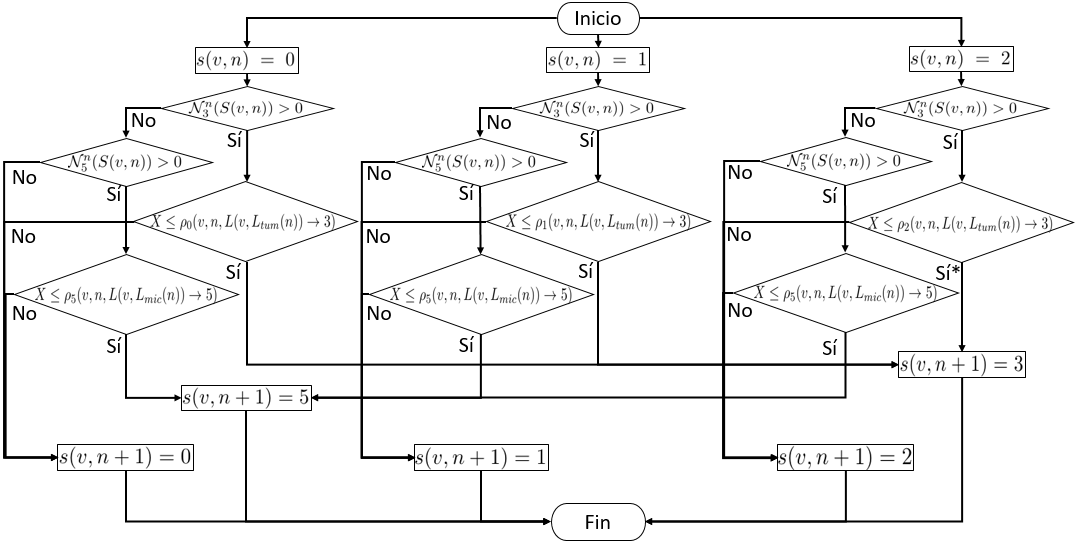
\includegraphics{img/fig-flux-diagram.png}}
\end{center}
\caption[Diagrama de flujo de las reglas del crecimiento tumoral y del crecimiento de las micromet\'astasis]{Diagrama de flujo de las reglas del crecimiento tumoral y del crecimiento de las micromet\'astasis. Se aprecian las distintas rutas que pueden tomar las c\'elulas normales del modelo para cambiar su estado al de una c\'elula cancer\'igena tumoral o a la de una micromet\'astasis en dependencia de las condiciones de su vecindad y del c\'alculo de las probabilidades de transici\'on. \textit{En el diagrama:} (*) Solo existen probabilidades de que ocurra durante la etapa vascular.}
\label{fig-flux-diagram}
\end{figure}

\subsubsection*{Reglas de la cascada metast\'asica}
 En las secciones~\ref{subsec-migrant}, \ref{subsec-migration} y \ref{subsec-metastasis} se sigui\'o un proceso gradual para la obtenci\'on de las reglas que representan la cascada metast\'asica, desde la aparici\'on de las c\'elulas migratorias, su desplazamiento a trav\'es del estroma, el transporte a trav\'es del sistema circulatorio y la creaci\'on de una nueva micromet\'astasis. A continuaci\'on se presenta un resumen de las reglas mencionadas de forma tal que se muestren como componentes integradores de la funci\'on de transici\'on local. Se expondr\'an las definiciones e hip\'otesis que se tuvieron en cuenta en cada caso para una r\'apida referencia. De esta forma tenemos el conjunto de reglas que reproducen la cascada metast\'asica como: 
\begin{equation*}
s(v,n+1)=\mathcal{R}(S(v,n))=\left\lbrace
	\begin{array}{ll}
		\zeta_2(v,n,L(v,L_{tum}(n))) & \textit{si } s(v,n)=2~\wedge~\mathcal{N}_3^n(S(v,n)) > 0 \\[0.2cm]
		\zeta_4(\mu(v,n)) & \textit{si } s(v,n)=4~\wedge~\mathcal{N}_{\mathcal{E}_{met}}^d(S(v,n))=0~\wedge\\
				         & \mathcal{N}_2^n(S(v,n))=0 \\
		2 & \textit{si } s(v,n)=4~\wedge~\mathcal{N}_{\mathcal{E}_{met}}^d(S(v,n))=0~\wedge\\
		  & \mathcal{N}_2^n(S(v,n))>0 \\[0.2cm]
		2 & \textit{si } s(v,n)=4~\wedge~\mathcal{N}_{\mathcal{E}_{met}}^d(S(v,n))>0
	\end{array}
\right..
\end{equation*}

La primera de estas reglas se corresponde con el \emph{surgimiento de c\'elulas migratorias}, de la que se realizan las siguientes anotaciones:\label{NOT-surgimiento-celulas-migratorias}

\paragraph*{{Fundamento biol\'ogico}:} La acumulaci\'on de mutaciones de las c\'elulas cancer\'igenas y los cambios en la matriz de interacci\'on intercelular provocados por la angiog\'enesis tumoral hacen posible que aparezcan c\'elulas con una reducida adhesi\'on celular y que expresan prote\'inas involucradas en el control de la movilidad y la supresi\'on de reguladores de la migraci\'on. Estos cambios solo se expresan en la etapa vascular del desarrollo tumoral. En la concepci\'on de estas reglas se adoptan de forma general las hip\'otesis I, II y VI que tratan sobre la progresi\'on idealizada del desarrollo tumoral, las mutaciones de las c\'elulas cancer\'igenas y la homogeneidad de las c\'elulas cancer\'igenas respectivamente.

\paragraph*{{Criterio de selecci\'on}:} Una c\'elula normal que pertenece al estroma expresado mediante la condici\'on $s(v,n)=2$ tiene una posibilidad de cambiar su estado al de una c\'elula migratoria del c\'ancer si en su vecindad inmediata existen c\'elulas pertenecientes a alg\'un tumor, expresado mediante la condici\'on $\mathcal{N}_3^n(S(v,n))>0$. Las funciones utilizadas son definidas en~\ref{def-cellstatus} y \ref{def-near-neighbours} respectivamente.

\paragraph*{{Funcionamiento}:} Para representar el surgimiento de estas c\'elulas hacemos que la variable aleatoria utilizada para reproducir la expansi\'on tumoral hacia el estroma pueda tomar el estado correspondiente con el de una c\'elula migratoria. De esta forma cuando el tumor est\'a en las \'ultimas instancias de su desarrollo en la etapa vascular al este crecer existe la posibilidad de que las nuevas c\'elulas cancer\'igenas se correspondan con el tipo migratorio. Luego si el criterio de selecci\'on de la regla se cumple, el valor del estado de la c\'elula $v$ en el instante de tiempo $n+1$ se determina a trav\'es de la variable aleatoria $\zeta_2(v,n,L(v,L_{tum}(n)))$ que puede tomar los valores:
\begin{align*}
\zeta_2(v,n,L(v,L_{tum}(n))) &\in \lbrace 2,3,4 \rbrace.
\end{align*}
Esta variable aleatoria posee la siguiente distribuci\'on de probabilidad:
\begin{align*}
P(\zeta_2(v,n,L(v,L_{tum}(n)))=2) &= 1 - \left[\rho_2(v,n,L(v,L_{tum}(n)) \rightarrow 3) + \rho_2(L(v,L_{tum}(n)) \rightarrow 4)\right], \\
P(\zeta_2(v,n,L(v,L_{tum}(n)))=3) &= \rho_2(v,n,L(v,L_{tum}(n)) \rightarrow 3), \\
P(\zeta_2(v,n,L(v,L_{tum}(n)))=4) &= \rho_2(L(v,L_{tum}(n)) \rightarrow 4).
\end{align*}
La probabilidad de transici\'on $\rho_2(v,n,L(v,L_{tum}(n)) \rightarrow 3)$ se utiliza para reproducir la expansi\'on tumoral, como se mostr\'o anteriormente, mientras que $\rho_2(L(v,L_{tum}(n)) \rightarrow 4)$ se utiliza para reproducir el surgimiento de c\'elulas migratorias. La extensi\'on de la concepci\'on cl\'asica de un aut\'omata celular que permite el uso de estas probabilidades de transici\'on se presenta en las definici\'on~\ref{prop-newlocal-func-3}. La expresi\'on para el c\'alculo de esta probabilidad de transici\'on, de acuerdo a la hip\'otesis XV sobre las situaciones de competencia entre tumores, se muestra a continuaci\'on:
\begin{equation*}
\rho_2(L(v,L_{tum}(n)) \rightarrow 4) = max\left[\rho_2(l_1 \rightarrow 4),\,\rho_2(l_2 \rightarrow 4),\ldots,\,\rho_2(l_m \rightarrow 4)\right].
\end{equation*}
En la expresi\'on anterior la funci\'on $L(v,L_{tum}(n))$ devuelve los tumores vecinos a la c\'elula $v$, como se muestra en la definici\'on~\ref{def-L-2}, donde $L_{tum}(n)$ contiene a las c\'elulas que forman cada tumor en la simulaci\'on, como se muestra en la definici\'on~\ref{def-L-n}. De ah\'i que $L(v,L_{tum}(n))=\lbrace l_1, l_2, \ldots, l_m \rbrace$ con $m=|L(v,L_{tum}(n))|$. De acuerdo a las hip\'otesis VIII y XIV sobre el desarrollo tumoral en funci\'on de la poblaci\'on y la interpretaci\'on de la neovasculatura respectivamente el c\'alculo de las probabilidades particulares $\rho_2(l \rightarrow 4)$ para cada tumor $l \in L(v,L_{tum}(n))$ se realiza mediante la expresi\'on siguiente:
\begin{equation*}
\rho_2(l \rightarrow 4) = (1-H(l,P_0^v)) \left( \displaystyle\frac{|l|}{K_v + K_{mig}} \right)^{\displaystyle 1/\eta_{mig}}.
\end{equation*}
Los par\'ametros $\eta_{mig} \in (0,1]$ y $K_{mig} \in \mathbb{N}$ nos permiten ajustar el comportamiento de la regla. Mediante la variaci\'on de $\eta_{mig}$ se puede variar el instante de tiempo en el que comienza el surgimiento de c\'elulas migratorias y la variaci\'on de $K_{mig}$ permite establecer un l\'imite para la probabilidad de surgimiento de dichas c\'elulas migratorias.\vspace*{0.5cm}

La segunda y tercera de estas reglas se corresponden con la \emph{migraci\'on}, de la que se realizan las siguientes anotaciones:\label{NOT-migracion}

\paragraph*{{Fundamento biol\'ogico}:} Una c\'elula cancer\'igena migratoria habiendo ingresado en el estroma procede a desplazarse a trav\'es del tejido mediante la degradaci\'on progresiva de la ECM hasta penetrar el sistema circulatorio en un posible punto de inserci\'on. El desplazamiento se produce aumentando progresivamente la distancia existente entre la c\'elula migratoria y la masa tumoral de la que se desprendi\'o porque esta toma la mayor\'ia de los nutrientes del entorno circundante y lo hace avanzando hacia la direcci\'on de donde provienen los nutrientes de la difusi\'on. Durante la migraci\'on existen tres situaciones fundamentales que pueden ocurrir: que la c\'elula migratoria posea destinos viables hacia los que desplazarse, que la c\'elula migratoria est\'e inm\'ovil y que la c\'elula migratoria est\'e en posici\'on de penetrar el sistema circulatorio ya que se encuentra en un posible punto de inserci\'on. La \'ultima situaci\'on se corresponde con el fin de la migraci\'on expresada en la cuarta regla relacionada con la cascada metast\'asica como se expondr\'a posteriormente. La concepci\'on de estas reglas se apoya en las hip\'otesis XVIII y XIX sobre la migraci\'on del c\'ancer y el sesgo direccional de la migraci\'on respectivamente.

\paragraph*{{Criterio de selecci\'on}:} Una c\'elula migratoria, expresado por la condici\'on $s(v,n)=4$, que no est\'e en posici\'on de penetrar el sistema circulatorio, expresado por la condici\'on $\mathcal{N}_{\mathcal{E}_{met}}^d(S(v,n))=0$ donde $\mathcal{E}_{met}=\lbrace 2,3,5 \rbrace$ son los destinos posibles de una met\'astasis, puede encontrarse en dos situaciones fundamentales: que est\'e inm\'ovil, expresado por la condici\'on $\mathcal{N}_2^n(S(v,n))=0$ en la segunda regla de la migraci\'on, o que posea destinos viables hacia los que desplazarse, expresado por la condici\'on $\mathcal{N}_2^n(S(v,n))>0$ en la tercera regla de la migraci\'on. Las funciones utilizadas son definidas en~\ref{def-cellstatus}, \ref{def-near-neighbours} y \ref{def-normal-distant-neighbours} respectivamente.

\paragraph*{{Funcionamiento}:} La actualizaci\'on de las c\'elulas migratorias en el presente aut\'omata celular se lleva a cabo en el m\'etodo $update-migratory-cells(G,\,C_{mig}^A(G),\,S(n),$ $\psi_{mig},\,\mu_{mig})$, mostrado en esta secci\'on en el algoritmo~\ref{alg-update-r-2}, en el que el orden en que son seleccionadas estas c\'elulas es aleatorio dada la naturaleza as\'incrona de la actualizaci\'on, donde los par\'ametros $\psi_{mig} \in [0,1]$ y $\mu_{mig} \in \mathbb{N}$ que se corresponden con una probabilidad de llevar a cabo un movimiento y el rango m\'aximo del propio movimiento respectivamente permiten la reproducci\'on de forma m\'as realista del movimiento de las c\'elulas cancer\'igenas, permitiendo desplazamientos con rangos variables, adem\'as de proporcionar un nuevo grado de ajuste al modelo. En caso de que se aplique la \emph{segunda regla} correspondiente con la de una c\'elula migratoria inm\'ovil se prueba su supervivencia haciendo el estado de la posici\'on actual igual al de la variable aleatoria $\zeta_4(\mu(v,n))$:
\begin{equation*}
s(v,n+1) = \zeta_4(\mu(v,n)).
\end{equation*}
Esta variable aleatoria puede tomar los siguientes valores:
\begin{equation*}
\zeta_4(\mu(v,n)) \in \lbrace 2,4 \rbrace.
\end{equation*}
Si toma valor $2$ se asume que la existencia de la c\'elula migratoria termin\'o y la posici\'on dejada por ella es ocupada por el estroma. Si toma valor $4$ la c\'elula migratoria contin\'ua con su existencia pero permanece inm\'ovil. Posee la siguiente distribuci\'on de probabilidad:
\begin{align*}
P(\zeta_4(\mu(v,n))=2) &= \rho_4(\mu(v,n) \rightarrow 2), \\
P(\zeta_4(\mu(v,n))=4) &= 1 - \rho_4(\mu(v,n) \rightarrow 2).
\end{align*}
La probabilidad de transici\'on $\rho_4(\mu(v,n) \rightarrow 2)$ se utiliza para determinar la supervivencia de la c\'elula migratoria. La extensi\'on de la concepci\'on cl\'asica de un aut\'omata celular que permite el uso de estas probabilidades de transici\'on se presenta en las definici\'on~\ref{prop-newlocal-func-4}. Se expresa como el cociente entre la distancia recorrida, determinada mediante la funci\'on $\mu(v,n)$, y la distancia promedio m\'axima $\mu_{max} \in \mathbb{N}$, es decir:
\begin{equation*}
\rho_4(\mu(v,n) \rightarrow 2) = \left(\displaystyle\frac{\mu(v,n)}{\mu_{max}} \right)^{\displaystyle 1 / \eta_{mig}'}.
\end{equation*}
El par\'ametro $\eta_{mig}' \in (0,1]$ nos permite ajustar el comportamiento de la regla. Mediante la variaci\'on de $\eta_{mig}'$ se pueden representar condiciones favorables o adversas para la supervivencia de la c\'elula migratoria. En caso de que se aplique la \emph{tercera regla} correspondiente con la existencia de destinos viables en la migraci\'on se utiliza una t\'ecnica conocida como intercambio de estados en teor\'ia de aut\'omatas celulares donde al actualizarse una part\'icula en movimiento se actualizan los estados de la posici\'on inicial y la final simult\'aneamente. El procedimiento se resume como: $(1)$ se le asigna a la posici\'on inicial $v$ de la c\'elula migratoria el estado $2$ mediante la aplicaci\'on de la regla; $(2)$ se selecciona una posici\'on destino $w$ mediante la aplicaci\'on de la funci\'on $d_{mig}(v,n)$; y $(3)$ se le asigna a la posici\'on destino elegida $w$ de la c\'elula migratoria el estado que tome la variable aleatoria $\zeta_4(\mu(v,n))$. Si la posici\'on destino toma el estado $2$ se considera que termin\'o la existencia de la c\'elula migratoria, en caso contrario si toma el estado $4$ se considera que el desplazamiento fue satisfactorio y la c\'elula contin\'ua con su existencia. La funci\'on $d_{mig}(v,n)$, definida en~\ref{def-dest-selection-2}, se plantea como:
\begin{equation*}
d_{mig}(v,n) = \left\lbrace
	\begin{array}{ll}
		v & \textit{si } |D_{mig}(v,n)|=0\\
		d_{mig}'(v,n) & \textit{si } |D_{mig}(v,n)|\neq 0		
	\end{array}
\right.. 
\end{equation*}
La funci\'on $D_{mig}(v,n)$, definida en~\ref{def-type-neighbours} devuelve los posibles destinos a los que puede desplazarse la c\'elula migratoria en cuesti\'on, siempre y cuando estos destinos la alejen del tumor donde se origin\'o, es decir:
\begin{equation*}
D_{mig}(v,n) = \lbrace w~|~w \in \mathcal{N}^n(v)~\wedge~s(w,n)=2~\wedge~o(v) = o(w)~\wedge~d_E(c_l,w) > d_E(c_l,v) \rbrace.
\end{equation*}
Si $d_{mig}(v,n) = v$ es porque no existen destinos viables hacia los que realizar la migraci\'on expresado por la condici\'on $|D_{mig}(v,n)|=0$, en caso contrario si $D_{mig}(v,n)= \lbrace w_1,w_2,\ldots,w_m \rbrace$ con $m = |D_{mig}(v,n)|$, es decir $|D_{mig}(v,n)|\neq 0$, el destino se elige mediante la funci\'on $d_{mig}'(v,n)$, que posee la siguiente expresi\'on:
\begin{equation*}
d_{mig}'(v,n) = \left\lbrace
	\begin{array}{ll}
		w_1 & \textit{con probabilidad } \frac{1}{m} \beta_{mig}(v,w_1)\\
		w_2 & \textit{con probabilidad } \frac{1}{m} \beta_{mig}(v,w_2)\\
		\vdots & \ldots\\
		w_m & \textit{con probabilidad } \frac{1}{m} \beta_{mig}(v,w_m)
	\end{array}\
\right..
\end{equation*}
Como se puede apreciar la probabilidad de que una posici\'on destino sea elegida satisfactoriamente depende de la funci\'on $\beta_{mig}(v,w)$, definida en~\ref{def-dest-selection}, y constituye de acuerdo a la hip\'otesis XIX sobre el sesgo direccional de la migraci\'on una forma de hacer que la migraci\'on se desarrolle hacia la vasculatura. Finalmente la posici\'on inicial $v$ y la posici\'on destino $w$ se actualizan con los valores correspondientes de acuerdo a lo planteado anteriormente:
\begin{align*}
s(v,n+1) &= 2,\\
s(w,n+1) &= \zeta_4(\mu(v,n)). 
\end{align*}\vspace*{0.5cm}

La regla final se corresponde con la \emph{met\'astasis}, de la que se realizan las siguientes anotaciones:\label{NOT-metastasis}

\paragraph*{{Fundamento biol\'ogico}:} Una c\'elula cancer\'igena migratoria que est\'e en presencia de un posible punto de intravasaci\'on procede a penetrar el sistema circulatorio para dar continuaci\'on a la cascada metast\'asica. Durante la estancia en el sistema circulatorio su existencia puede ser terminada por el sistema inmunitario o como consecuencia del estr\'es mec\'anico sufrido. Eventualmente se adhieren a un posible punto de extravasaci\'on en el que degradan la pared del vaso sangu\'ineo y abandona el sistema circulatorio. La concepci\'on de esta regla se apoya en las hip\'otesis XX y XXI sobre las conexiones distantes del grafo y los destinos viables de la met\'astasis.

\paragraph*{{Criterio de selecci\'on}:} Una c\'elula migratoria, expresado por la condici\'on $s(v,n)=4$, que est\'e en posici\'on de penetrar el sistema circulatorio, expresado por la condici\'on $\mathcal{N}_{\mathcal{E}_{met}}^d(S(v,n))>0$ donde $\mathcal{E}_{met}=\lbrace 2,3,5 \rbrace$ son los destinos posibles de una met\'astasis, abandona su posici\'on y pasa a pertenecer al conjunto de actualizaci\'on as\'incrono $C_{sc}^A(G)$ donde permanecer\'a por un per\'iodo de tiempo, hasta que lo abandone satisfactoriamente en la posici\'on destino.

\paragraph*{{Funcionamiento}:} La penetraci\'on del sistema circulatorio puede ocurrir en dos localizaciones: en un capilar sangu\'ineo distante de la masa tumoral al que arriban las c\'elulas cancer\'igenas despu\'es de llevar a cabo la migraci\'on a trav\'es del estroma, y en un capilar sangu\'ineo que pertenezca al interior del tumor producto de la angiog\'enesis. La primera de estas situaciones es tratada mediante la regla de la met\'astasis que se expone a continuaci\'on, mientras que la segunda situaci\'on se trata mediante el m\'etodo $update-tumor-migratory-cells(G,\,C_{tum}^A(G),\,C_{sc}^A(G),\,S(n))$ del procedimiento de actualizaci\'on, presentado en esta secci\'on en~\ref{alg-update-r-3}. La regla es determinista en el sentido de que si se cumple el criterio de selecci\'on, la c\'elula migratoria siempre abandona su posici\'on y penetra el sistema circulatorio, es decir, pasa a pertenecer al conjunto de actualizaci\'on as\'incrono $C_{sc}^A(G)$ con la informaci\'on referente a su destino y con un tiempo de transporte igual a cero. El destino de la met\'astasis se elige de forma aleatoria a trav\'es de la funci\'on $d_{met}(v,n)$, definida en~\ref{def-dest-selection-met}, cuya expresi\'on es la siguiente:
\begin{figure}[t!]
\begin{center}
\scalebox{0.52}{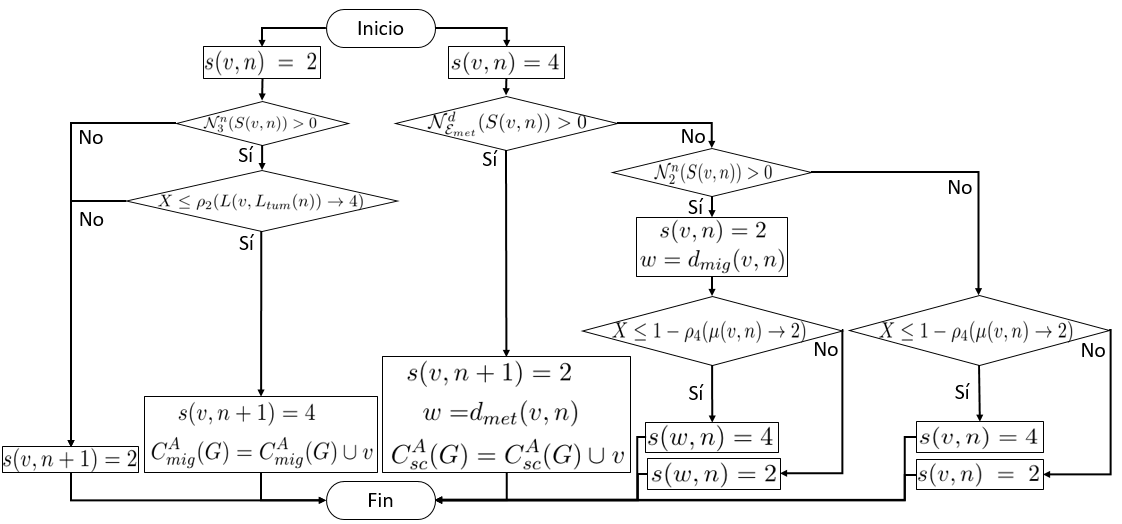
\includegraphics{img/fig-flux-diagram-2.png}}
\end{center}
\caption[Diagrama de flujo de las reglas de la aparici\'on de c\'elulas migratorias, migraci\'on y met\'astasis]{Diagrama de flujo de las reglas de la aparici\'on de c\'elulas migratorias, migraci\'on y met\'astasis. Se aprecian la situaci\'on que provoca la aparici\'on de c\'elulas migratorias en la frontera del tumor, las situaciones que pueden darse durante la migraci\'on de estas c\'elulas cancer\'igenas y algunos detalles de c\'omo se lleva a cabo la selecci\'on de los destinos de la misma y de la met\'astasis.}
\label{fig-flux-diagram-2}
\end{figure}
\begin{equation*}
d_{met}(v,n) = \left\lbrace
	\begin{array}{ll}
		w_1 & \textit{con probabilidad } 1/m\\
		w_2 & \textit{con probabilidad } 1/m\\
		\vdots & \ldots\\
		w_m & \textit{con probabilidad } 1/m
	\end{array}
\right..
\end{equation*}
La funci\'on $D_{met}(v,n)$, definida en~\ref{def-type-neighbours-2}, que devuelve el conjunto compuesto por los posibles destinos de la met\'astasis $\lbrace w_1, w_2, \ldots, w_m \rbrace$ con $m = |D_{met}(v,n)|$ posee la siguiente expresi\'on:
\begin{equation*}
D_{met}(v,n) = \lbrace w~|~w \in \mathcal{N}^d(v)~\wedge~s(w,n) \in \mathcal{E}_{met} \rbrace.
\end{equation*}
El m\'etodo $update-tumor-migratory-cells(G,\,C_{tum}^A(G),\,C_{sc}^A(G),\,S(n))$ es an\'alogo al proceso realizado por la migraci\'on: el orden de actualizaci\'on se define de forma aleatoria, se eval\'ua la probabilidad de que la c\'elula tumoral que est\'a en presencia del capilar sangu\'ineo produzca una descendencia migratoria mediante el m\'etodo $get-probability(v)$ equivalente a la funci\'on $\rho_2(l \rightarrow 4)$ definida en~\ref{eq-migrant-2} y \ref{eq-migrant-3}, se selecciona el destino de la met\'astasis mediante el m\'etodo $select-destiny-vertex(v,\,S(n),\,G)$ equivalente a la funci\'on $d_{met}(v,n)$, y finalmente se a\~nade la descendencia migratoria al sistema circulatorio mediante el m\'etodo $add-cell-to-bloodstream(v,\,d,\,C_{sc}^A(G))$. El m\'etodo $update-migratory-cells-in-bloodstream(C_{sc}^A(G),\,\psi_{met0},\,\psi_{met1},\,T_{sc},\,\xi_{sc})$, presentado en esta secci\'on en~\ref{alg-update-r-1}, es el encargado de actualizar el conjunto as\'incrono $C_{sc}^A(G)$ que contiene las c\'elulas migratorias que residen en el torrente sangu\'ineo, evaluando su supervivencia y su arribo a la localizaci\'on destino, determinando si se crea satisfactoriamente una nueva micromet\'astasis. En la figura~\ref{fig-flux-diagram-2} se representan las reglas de la migraci\'on y met\'astasis en un diagrama de flujo. Al igual que en el diagrama de flujo de las reglas de la conservaci\'on del estado de las c\'elulas normales, del crecimiento tumoral y del crecimiento de las micromet\'astasis, se utiliza una variable aleatoria $X$ que posee una distribuci\'on uniforme en $[0,1]$. 

\newpage
\chapter{Par\'ametros relacionados con la simulaci\'on computacional}
\label{sec-validation}
La validaci\'on posee una importancia crucial en el proceso de concepci\'on de un modelo matem\'atico-computacional pues constituye la verificaci\'on de su robustez, de su capacidad predictiva y de la veracidad de las hip\'otesis planteadas. Entre los distintos temas que se deben abordar en esta secci\'on se encuentran el an\'alisis de los valores asignados a los par\'ametros del modelo y las repercusiones de sus posibles variaciones, mientras que la comparaci\'on de los resultados num\'ericos y visuales obtenidos con datos provenientes de distintas investigaciones \textit{in vitro}, \textit{in vivo} y estudios cl\'inicos se realizar\'a en la secci\'on~\ref{sec-results}. Una configuraci\'on de la simulaci\'on comprende todos los par\'ametros cuyos valores son requeridos para la ejecuci\'on del aut\'omata celular. Es importante destacar que la totalidad del modelo est\'a concebido para reproducir el desarrollo de cualquier tipo de carcinoma, pero como se podr\'a apreciar en las secciones restantes nos concentramos en el carcinoma ductal infiltrante que constituye el caso m\'as frecuente del c\'ancer de mama. Entre las razones detr\'as de la elecci\'on est\'a la mayor abundancia de informaci\'on y datos respecto a este tipo de c\'ancer.

\section{Par\'ametros de la construcci\'on de la red y de la ley de crecimiento log\'istico}
\label{subsec-network-param}
Los par\'ametros de construcci\'on de la red se corresponden con los argumentos del algoritmo~\ref{alg-watts} mostrado en la secci\'on~\ref{subsec-watts-2}, y determinan el tama\~no del espacio que se utiliza para representar las localizaciones donde se desarrolla el c\'ancer. Se presentan en el cuadro~\ref{table-network-params} que aparece a continuaci\'on para una r\'apida referencia. Los par\'ametros de la ley de crecimiento log\'istico se utilizan para reproducir el crecimiento tumoral, espec\'ificamente en las reglas presentadas en las secciones~\ref{subsec-celldiv} y \ref{subsec-micrometastasis} obtenidas a trav\'es de un proceso de inferencia de la regla a partir de dicha ley continua. Se presentan en el cuadro~\ref{table-logistic-params} para una r\'apida referencia.

\begin{table}[!ht]
\begin{center}
\scalebox{0.9}{\begin{tabular}{|p{2cm}|p{14.5cm}|} \hline
\emph{Par\'ametro} & \emph{Descripci\'on} \\\hline
\multicolumn{1}{|c|}{$s_x$, $s_y$} & Dimensiones del espacio declarado. Las componentes espaciales de los v\'ertices del grafo poseen los siguientes rangos de valores: $0 \leq x < s_x$ y $0 \leq y < s_y$. \\\hline
\multicolumn{1}{|c|}{$s_o$} & Valor que marca la divisi\'on de la red entre un \'organo y el otro. Posee el siguiente rango de valores: $0 \leq s_o < s_x$. Generalmente toma valor $s_o = s_x / 2$. \\\hline
\multicolumn{1}{|c|}{$p$} & Probabilidad de reconexi\'on del modelo Watts-Strogatz. \\\hline
\end{tabular}}\vspace*{-0.5cm}
\end{center}
\caption[Par\'ametros de la construcci\'on de la red utilizados por el modelo Watts-Strogatz]{Par\'ametros de la construcci\'on de la red utilizados por el modelo Watts-Strogatz.}
\label{table-network-params}
\end{table}

\begin{table}[!ht]
\begin{center}
\scalebox{0.9}{\begin{tabular}{|p{2cm}|p{14.5cm}|} \hline
\emph{Par\'ametro} & \emph{Descripci\'on} \\\hline
\multicolumn{1}{|c|}{$P_0^a$, $P_0^v$} & Poblaciones iniciales de las etapas avascular y vascular respectivamente. \\\hline
\multicolumn{1}{|c|}{$r_a$, $r_v$} & Ritmos de proliferaci\'on de las etapas avascular y vascular respectivamente. \\\hline
\multicolumn{1}{|c|}{$K_a$, $K_v$} & Capacidad de carga de las etapas avascular y vascular respectivamente. \\\hline
\multicolumn{1}{|c|}{$\Delta t$} & Tiempo transcurrido entre los instantes de tiempo $n$ y $n+1$. \\\hline
\multicolumn{1}{|c|}{$n_a$} & Tiempo que permanece un tumor en etapa avascular. \\\hline
\end{tabular}}\vspace*{-0.5cm}
\end{center}
\caption[Par\'ametros correspondientes con la ley de crecimiento log\'istico]{Par\'ametros correspondientes con la ley de crecimiento log\'istico.}
\label{table-logistic-params}
\end{table}

En la secci\'on~\ref{subsec-macro} se expuso que un tumor avascular solo puede crecer hasta un radio de $R_a \in [0$.$5, 1]mm$. Asumiendo que un tumor tiene forma esf\'erica se estima que el volumen ocupado por el mismo durante la etapa avascular posee un valor perteneciente al intervalo $V_a \in [0$.$5236, 4$.$189]mm^3$. En~\cite{breastdata,chile} se estima que el radio de un tumor vascular correspondiente con un carcinoma ductal infiltrante puede tener valores de $R_v \in [10, 15]mm$. Siguiendo la idea anterior se estima que el volumen ocupado por un tumor vascular de estas dimensiones posee un valor perteneciente al intervalo $V_v \in [4$.$189 \times 10^3, 1$.$414 \times 10^4]mm^3$. El radio de una c\'elula cancer\'igena toma un valor del siguiente intervalo $R_c \in [1$.$5 \times 10^{-2}, 2$.$0 \times 10^{-2}]mm$ tomando en cuenta los tipos m\'as comunes de carcinomas~\cite{kansal3,breastdata,vajtai}. En~\cite{wisconsin} este valor se estima en $R_c \approx 17$.$46 \mu m$, utilizando en el c\'alculo $212$ muestras de c\'elulas obtenidas de tumores del tipo carcinoma ductal infiltrante, que constituye la forma m\'as com\'un de c\'ancer de mama. Asumiendo que una c\'elula tiene forma esf\'erica se determina su volumen aproximado como $V_{c} \in [1$.$414 \times 10^{-5}, 3$.$351 \times 10^{-5}]mm^3$. Utilizando los intervalos de valores del volumen de la c\'elula cancer\'igena y de un tumor durante las etapas avascular y vascular se pueden determinar las capacidades de carga del entorno para ambas etapas, devolviendo los siguientes intervalos $K_a \in [1$.$563 \times 10^4, 2$.$963 \times 10^5]$ y $K_v \in [1$.$25 \times 10^8, 1$.$0 \times 10^9]$. 

Los intervalos de valores antes mencionados son los que se requieren para una simulaci\'on que se lleve a cabo en tres dimensiones, pero dado que el presente modelo solo utiliza dos de estas, es necesario realizar una serie de transformaciones adicionales. Como se expres\'o en la hip\'otesis XII sobre la representaci\'on del tejido el modelo se concibe como una reproducci\'on de un corte de tejido como se aprecia en la figura~\ref{fig-transformation}. Se infiere que se debe asumir que dicho corte se corresponde con una circunferencia con radio igual al del tumor en cualquiera de sus etapas. De esta forma tenemos que el \'area ocupada por un tumor avascular pertenece al intervalo $A_a \in [7$.$854 \times 10^{-1}, 3$.$142]mm^2$ y el de un tumor vascular pertenece al intervalo $A_v \in [3$.$142 \times 10^2, 7$.$069 \times 10^2]mm^2$. Siguiendo el mismo an\'alisis se asume que una secci\'on de una c\'elula posee una forma semejante a una circunferencia, por lo que utilizando el radio de una c\'elula cancer\'igena se puede obtener la superficie ocupada por dicha secci\'on, devolviendo un valor que pertenece al intervalo $A_c \in [7$.$069 \times 10^{-4}, 1$.$257 \times 10^{-3}]mm^2$. Finalmente, las capacidades de carga para las etapas avascular y vascular poseen valores que pertenecen a los intervalos $K_a \in [6$.$25 \times 10^2, 4$.$444 \times 10^3]$ y $K_v \in [2$.$5 \times 10^5, 1$.$0 \times 10^6]$. En el cuadro~\ref{table-original-values} aparecen recogidos los datos mencionados anteriormente para una r\'apida referencia.

\begin{figure}[!ht]
\begin{center}
\scalebox{0.45}{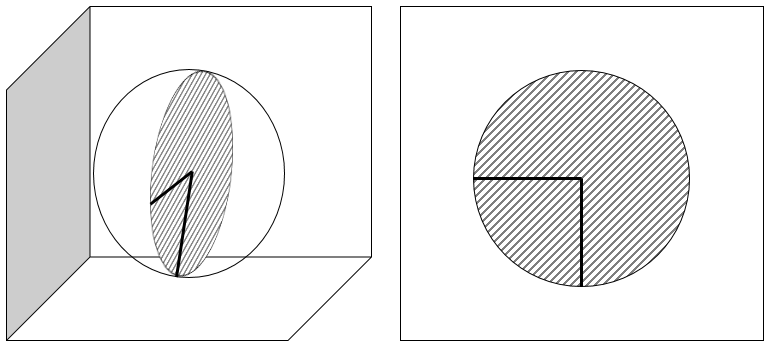
\includegraphics{img/transformation.png}}
\end{center}\vspace*{-0.75cm}
\caption[Transformaci\'on de la representaci\'on de un tumor en tres dimensiones a dos dimensiones]{Transformaci\'on de la representaci\'on de un tumor en tres dimensiones a dos dimensiones. Se observa el uso de la secci\'on o corte de la esfera que presenta mayor \'area.}
\label{fig-transformation}
\end{figure}

\begin{table}[!ht]
\begin{center}
\scalebox{0.9}{\begin{tabular}{|c|c|c|c|c|} \hline
\multicolumn{2}{|c|}{\emph{Datos}} & \multicolumn{1}{|l|}{\emph{M\'inimo}} & \multicolumn{1}{|l|}{\emph{M\'aximo}} & \multicolumn{1}{|l|}{\emph{Promedio}}\\\hline

 & \multicolumn{1}{|l|}{$R_c(mm)$} & \multicolumn{1}{|c|}{$1$.$5 \times 10^{-2}$} & \multicolumn{1}{|c|}{$2$.$0 \times 10^{-2}$} & \multicolumn{1}{|c|}{$1$.$75 \times 10^{-2}$} \\\cline{2-5}                              
\emph{C\'elula cancer\'igena} & \multicolumn{1}{|l|}{$V_c(mm^3)$} & \multicolumn{1}{|c|}{$1$.$414 \times 10^{-5}$} & \multicolumn{1}{|c|}{$3$.$351 \times 10^{-5}$} & \multicolumn{1}{|c|}{$2$.$2244 \times 10^{-5}$} \\\cline{2-5} 
 & \multicolumn{1}{|l|}{$A_c(mm^2)$} & \multicolumn{1}{|c|}{$7$.$069 \times 10^{-4}$} & \multicolumn{1}{|c|}{$1$.$257 \times 10^{-3}$} & \multicolumn{1}{|c|}{$9$.$621 \times 10^{-4}$} \\\hline
                              
 & \multicolumn{1}{|l|}{$R_a(mm)$} & \multicolumn{1}{|c|}{$0$.$5$} & \multicolumn{1}{|c|}{$1$} & \multicolumn{1}{|c|}{$7$.$5 \times 10^{-1}$} \\\cline{2-5}
 & \multicolumn{1}{|l|}{$V_a(mm^3)$} & \multicolumn{1}{|c|}{$5$.$236 \times 10^{-1}$} & \multicolumn{1}{|c|}{$4$.$189$} & \multicolumn{1}{|c|}{$1$.$767$} \\\cline{2-5} 
\emph{Tumor avascular} & \multicolumn{1}{|l|}{$K_a$*} & \multicolumn{1}{|c|}{$1$.$563 \times 10^4$} & \multicolumn{1}{|c|}{$2$.$963 \times 10^5$} & \multicolumn{1}{|c|}{$7$.$872 \times 10^4$} \\\cline{2-5} 
 & \multicolumn{1}{|l|}{$A_a(mm^2)$} & \multicolumn{1}{|c|}{$7$.$854 \times 10^{-1}$} & \multicolumn{1}{|c|}{$3$.$142$} & \multicolumn{1}{|c|}{$1.767$} \\\cline{2-5} 
 & \multicolumn{1}{|l|}{$K_a$**} & \multicolumn{1}{|c|}{$6$.$25 \times 10^2$} & \multicolumn{1}{|c|}{$4$.$444 \times 10^3$} & \multicolumn{1}{|c|}{$1$.$837 \times 10^3$} \\\hline
					   
 & \multicolumn{1}{|l|}{$R_v(mm)$} & \multicolumn{1}{|c|}{$1$.$0 \times 10^1$} & \multicolumn{1}{|c|}{$1$.$5 \times 10^1$} & \multicolumn{1}{|c|}{$1$.$25 \times 10^1$} \\\cline{2-5}
 & \multicolumn{1}{|l|}{$V_v(mm^3)$} & \multicolumn{1}{|c|}{$4$.$189 \times 10^3$} & \multicolumn{1}{|c|}{$1$.$414 \times 10^4$} & \multicolumn{1}{|c|}{$8$.$181 \times 10^3$} \\\cline{2-5} 
\emph{Tumor vascular} & \multicolumn{1}{|l|}{$K_v$*} & \multicolumn{1}{|c|}{$1$.$25 \times 10^8$} & \multicolumn{1}{|c|}{$1$.$0 \times 10^9$}& \multicolumn{1}{|c|}{$3$.$644 \times 10^8$} \\\cline{2-5} 
 & \multicolumn{1}{|l|}{$A_v(mm^2)$} & \multicolumn{1}{|c|}{$3$.$142 \times 10^2$} & \multicolumn{1}{|c|}{$7$.$069 \times 10^2$} & \multicolumn{1}{|c|}{$4$.$909 \times 10^2$}\\\cline{2-5} 
 & \multicolumn{1}{|l|}{$K_v$**} & \multicolumn{1}{|c|}{$2$.$5 \times 10^5$} & \multicolumn{1}{|c|}{$1$.$0 \times 10^6$} & \multicolumn{1}{|c|}{$5$.$102 \times 10^5$}\\\hline
\end{tabular}}\vspace*{-0.5cm}
\end{center}
\caption[Datos de las caracter\'isticas f\'isicas como el radio y vol\'umen de la c\'elula cancer\'igena, de un tumor en etapa avascular y vascular, y de la superficie que ocupa un corte transversal de los mismos]{Datos de las caracter\'isticas f\'isicas como el radio y vol\'umen de la c\'elula cancer\'igena, de un tumor en etapa avascular y vascular, y de la superficie que ocupa un corte transversal de los mismos, correspondientes con el tipo de c\'ancer de mama conocido como carcinoma ductal infiltrante. \emph{En el cuadro:} (*) Capacidad de carga con respecto al volumen; (**) Capacidad de carga con respecto a la superficie ocupada por el corte transversal.}
\label{table-original-values}
\end{table} 

Las localizaciones donde se reproduce el ciclo vital tumoral deben poseer el espacio suficiente para contener varias lesiones neopl\'asicas, motivo por el que se representa un corte de tejido de dimensiones $[0,10]cm \times [0,5]cm$, donde las porciones $[0,5]cm \times [0,5]cm$ y $[5,10]cm \times [0,5]cm$ se corresponden con el \'organo primario y secundario respectivamente. Las dimensiones de este espacio con respecto al n\'umero de c\'elulas contenidas se estima mediante el radio promedio de una c\'elula cancer\'igena $R_c$, quedando un espacio de dimensiones $[0, 3000] \times [0, 1500]$ aproximadamente, para un total de $4$.$5 \times 10^6$ c\'elulas. Por tanto, los par\'ametros de construcci\'on de la red de las dimensiones del espacio declarado poseen los siguientes valores $s_x = 3000$ y $s_y = 1500$, mientras que la divisi\'on entre los \'organos es $s_o = 1500$. Como se expuso en la secci\'on~\ref{subsec-watts-2} la probabilidad de reconexi\'on de la red posee el siguiente rango de valores $p \in [10^{-3},10^{-2}]$.

Los par\'ametros que restan por definir son los ritmos de proliferaci\'on tumoral $r_a$ y $r_v$, y la cantidad de tiempo que transcurre entre el instante de tiempo $n$ y el $n+1$, o sea $\Delta t$. Los valores de estos par\'ametros espec\'ificos a la ley de crecimiento log\'istico no han sido analizados hasta este momento en ning\'un trabajo previo, por lo que sus valores ser\'an estimados con el objetivo de ajustar el comportamiento del aut\'omata celular y que reproduzca en la mayor medida posible los procesos que lleva a cabo el c\'ancer en la realidad. En la secci\'on~\ref{subsec-celldiv} se llev\'o a cabo un procedimiento que ten\'ia como objetivo lograr que los valores de la probabilidad de crecimiento tumoral, mostrados en las expresiones~(\ref{eq-pa}) y~(\ref{eq-pv}), estuviese acotada en el intervalo $[0,\rho_{max}]$, donde $\rho_{max}$ es un valor de probabilidad m\'aximo seleccionado a priori y que funciona como un mecanismo de ajuste. En~\cite{ruben} el valor m\'aximo alcanzado por la probabilidad de crecimiento tumoral es de aproximadamente $0$.$63$, mientras que en~\cite{kansal,kansal3} esta probabilidad var\'ia entre $0$.$192$ y $0$.$384$, lo cual nos otorga una medida para ajustar nuestra funci\'on de probabilidad. Este procedimiento culmin\'o con la obtenci\'on de la expresi\'on n\'umero~(\ref{eq-cond-1}) que asegura que dicha distribuci\'on de probabilidad est\'e acotada en el intervalo mencionado, pero que ofrece una metodolog\'ia para estimar los valores de $r_a$ y $r_v$. Seg\'un dicha condici\'on:
\begin{subequations}
\begin{equation*}
r_a \in \left[0, \frac{4 \rho_{max}^a}{K_a}\right],~r_v \in \left[0, \frac{4 \rho_{max}^v}{K_v}\right],
\end{equation*}
\end{subequations}
donde los valores de $K_a$ y $K_v$ fueron determinados anteriormente. El valor m\'aximo alcanzable de probabilidad se obtiene al hacer $\rho_{max}^a= K_a r_a / 4 = 1$ y $\rho_{max}^v= K_v r_v / 4 = 1$, que a su vez se obtiene cuando~(\ref{eq-cond-t}):
\begin{equation}
t = \frac{1}{r} \ln\frac{K-P_0}{P_0}
\end{equation}
donde si hacemos $t=n\Delta t$ obtenemos:
\begin{equation}
n = \frac{1}{r\Delta t} \ln\frac{K-P_0}{P_0}. \label{final}
\end{equation}

De esta expresi\'on~(\ref{final}) se infiere que el $\Delta t$ determina el punto donde la distribuci\'on de probabilidad alcanza su m\'aximo, dato relevante ya que esta distribuci\'on posee una curva semejante a la funci\'on gaussiana. De esta forma si conocemos el tiempo total que ocupa las etapas avascular o vascular dentro del ciclo de vida del tumor es posible ajustar esta distribuci\'on a los incrementos de tama\~no que presenta un tumor en ambas etapas. Se hace que el valor de $\Delta t$ se corresponda con un tiempo de $24$ horas. De esta forma el n\'umero de generaciones del aut\'omata coincide con la cantidad de d\'ias que est\'a simulando. En las gr\'aficas~\ref{graph-probability-distribution-avascular} se muestran las distribuciones de probabilidad de las funciones $\rho_a(n\Delta t)$~(\ref{eq-pa}) y $\rho_v(n\Delta t)$~(\ref{eq-pv}) que describen el crecimiento tumoral durante las etapas avascular y vascular respectivamente, tomando como lapso de tiempo $365$ d\'ias para ambas etapas. Como se puede apreciar el tiempo se toma relativo al inicio de la etapa.
\begin{figure}[!ht]
\begin{center}
\subfigure[Etapa avascular $P_0^a = 1$, $K_a = 2$.$5 \times 10^3$]{\scalebox{0.88}{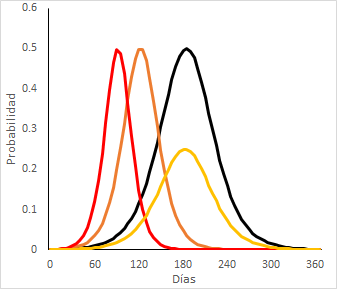
\includegraphics{img/graphs/graph-prob-avascular-3x4.png}}}
\subfigure[Etapa vascular $P_0^v = 2$.$5 \times 10^3$, $K_v = 6$.$3 \times 10^5$]{\scalebox{0.88}{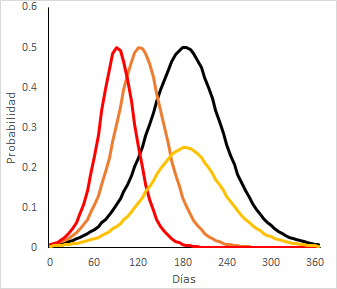
\includegraphics{img/graphs/graph-prob-vascular-3x4.png}}}
\end{center}\vspace*{-0.5cm}
\caption[Distribuciones de probabilidad de las funciones $\rho_a(n\Delta t)$ y $\rho_v(n\Delta t)$ que describen el crecimiento tumoral para distintos par\'ametros]{Distribuciones de probabilidad de las funciones $\rho_a(n\Delta t)$ y $\rho_v(n\Delta t)$ que describen el crecimiento tumoral durante las etapas avascular y vascular. (a) En negro $r_a=8$.$0 \times 10^{-4}$, $\Delta t = 53$; en naranja $r_a=8$.$0 \times 10^{-4}$, $\Delta t = 80$; en rojo $r_a=8$.$0 \times 10^{-4}$, $\Delta t = 107$; y en amarillo $r_a=4$.$0 \times 10^{-4}$, $\Delta t = 107$. (b) En negro $r_v=3$.$2 \times 10^{-6}$, $\Delta t = 9$.$4 \times 10^{3}$; en naranja $r_v=3$.$2 \times 10^{-6}$, $\Delta t = 1$.$4 \times 10^{4}$; en rojo $r_v=3$.$2 \times 10^{-6}$, $\Delta t = 1$.$9 \times 10^{4}$; y en amarillo $r_v=1$.$6 \times 10^{-6}$, $\Delta t = 1$.$9 \times 10^{4}$.}
\label{graph-probability-distribution-avascular}
\end{figure}

De estas gr\'aficas se puede inferir que seg\'un el modelo de crecimiento log\'istico la m\'axima velocidad de expansi\'on tumoral se presenta en los momentos centrales del lapso de tiempo correspondiente con cada etapa. Si se logra confirmar este hecho cl\'inicamente puede constituir una predici\'on importante ya que dadas dos observaciones del crecimiento tumoral que permitan determinar la velocidad de expansi\'on del tumor se puede determinar el momento en que transcurre su desarrollo y con este se puede determinar el tiempo que le toma alcanzar un tama\~no que ponga en peligro la vida del paciente.

\section{Par\'ametros de la asignaci\'on de estados iniciales y de los vectores de nutrientes}
\label{subsec-states-param}
Los par\'ametros de la asignaci\'on de estados iniciales se corresponden con la disposici\'on inicial de los estados en la simulaci\'on para representar un corte de tejido de las localizaciones donde se desarrolla el c\'ancer. El presente modelo est\'a orientado a representar el crecimiento de tumores que surgen en el epitelio correspondiente con el tipo de c\'ancer conocido como carcinoma. En la secci\'on anterior~\ref{subsec-network-param} se expuso que las simulaciones est\'an dirigidas a reproducir espec\'ificamente el carcinoma ductal infiltrante que surge en el epitelio que recubre los conductos mamarios, motivo por el que se conciben varios esquemas de asignaci\'on de estados iniciales: el primero para reproducir un corte de tejido gen\'erico donde se aprecien tres capas correspondientes con el lumen, el epitelio y el estroma, es decir, un corte que abarca tanto la superficie del \'organo como el interior; el segundo reproduce un corte de tejido correspondiente con una secci\'on del ducto mamario; mientras que el tercero reproduce un corte de tejido comprendido enteramente por estroma correspondiente al interior de un \'organo. Los esquemas I y II se utilizan fundamentalmente para representar el \'organo primario, mientras que el III para el \'organo secundario. En la figura~\ref{fig-initial-states-diagrams} se pueden apreciar dichos esquemas de asignaci\'on de estados iniciales.

\begin{figure}[!ht]
\begin{center}
\scalebox{0.5}{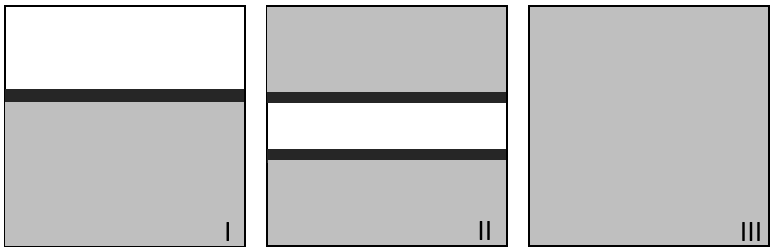
\includegraphics{img/fig-initial-states-diagrams.png}}
\end{center}\vspace*{-0.75cm}
\caption[Diagramas mostrando los esquemas de asignaci\'on de los estados iniciales]{Diagramas mostrando los esquemas de asignaci\'on de los estados iniciales. La asignaci\'on de colores es: blanco para el lumen, negro para el epitelio y gris para el estroma. }
\label{fig-initial-states-diagrams}
\end{figure}

Un elemento distintivo de la asignaci\'on de los estados iniciales es el tipo de tejido epitelial ya que el cuerpo humano cuenta con distintos tipos de epitelio en dependencia del \'organo representado, con disposiciones celulares y grosor distintos. En el ap\'endice~\ref{app-d} aparecen resumidos los distintos tipos de epitelios presentes en el cuerpo humano al igual que la figura~\ref{fig-epitheliums} que muestra los diagramas de estos tejidos~\cite{robins}. Dado que el aut\'omata celular reproduce las localizaciones que pueden ser ocupadas por c\'elulas cancer\'igenas se debe dividir el grosor del epitelio entre el tama\~no de una localizaci\'on representada. Una c\'elula del aut\'omata posee dimensiones aproximadas de $[0,3$.$5 \times 10^{-2}]mm \times [0,3$.$5 \times 10^{-2}]mm$ ya que se corresponden con las localizaciones que pueden ser ocupadas por una c\'elula cancer\'igena de un carcinoma ductal infiltrante. Los ductos mamarios constituyen estructuras tubulares con di\'ametro variable entre $0$.$1mm$ y $1mm$, revestidos por epitelio c\'ubico simple compuesto por una capa de c\'elulas de grosor equivalente al de una c\'elula cancer\'igena $3$.$5 \times 10^{-2}mm$. Por tanto la representaci\'on de este epitelio en el aut\'omata tambi\'en posee una \'unica capa de c\'elulas, es decir $o_e=1$. En los cuadros~\ref{table-states-params-1} y~\ref{table-states-params-2} aparecen recogidos los par\'ametros necesarios para la asignaci\'on de los estados iniciales de los esquemas I y II, exceptuando el III ya que est\'a compuesto enteramente por estroma.

\begin{table}[!ht]
\begin{center}
\scalebox{0.9}{\begin{tabular}{|p{2cm}|p{14.5cm}|} \hline
\emph{Par\'ametro} & \emph{Descripci\'on} \\\hline
\multicolumn{1}{|c|}{$o_l$} & Cantidad de capas del lumen.\\\hline
\multicolumn{1}{|c|}{$o_e$} & Cantidad de capas del epitelio. \\\hline
\multicolumn{1}{|c|}{$o_s$} & Cantidad de capas del estroma. Se determina como la cantidad de capas restantes en la red una vez que se disponen el lumen y el epitelio, es decir $o_s=s_y - (o_l + o_e)$.\\\hline
\multicolumn{1}{|c|}{$v_x^t$, $v_y^t$} & Coordenadas de la c\'elula cancer\'igena central del tumor inicial. La disposici\'on inicial del tumor se determina a partir de las coordenadas de esta c\'elula central. Se asume que la coordenada $v_y^t$ pertenece al siguiente rango de valores: $v_y^t \in [o_l, o_l + o_e]$, y generalmente $v_x^t = s_x/4$. \\\hline
\end{tabular}}\vspace*{-0.5cm}
\end{center}
\caption[Par\'ametros utilizados en la asignaci\'on de los estados iniciales a las c\'elulas del aut\'omata seg\'un el primer esquema]{Par\'ametros utilizados en la asignaci\'on de los estados iniciales a las c\'elulas del aut\'omata seg\'un el primer esquema.}
\label{table-states-params-1}
\end{table}

\begin{table}[!ht]
\begin{center}
\scalebox{0.9}{\begin{tabular}{|p{2cm}|p{14.5cm}|} \hline
\emph{Par\'ametro} & \emph{Descripci\'on} \\\hline
\multicolumn{1}{|c|}{$o_e$} & Cantidad de capas del epitelio.\\\hline
\multicolumn{1}{|c|}{$o_d$} & Coordenada de la l\'inea central del ducto mamario. Se extiende por los puntos $(v_x,o_d)$ para todo $v \in V(G)$.\\\hline
\multicolumn{1}{|c|}{$R^d$} & Radio del ducto mamario representado. Se itera por los v\'ertices $v \in V(G)$ de coordenadas $v = (v_x,v_y)$ y seg\'un la distancia euclideana~(Def. \ref{def-euclidean-distance}) entre dicho v\'ertice y su correspondiente en la l\'inea central del ducto mamario $v^d = (v_x,o_d)$ se le asigna uno de los estados correspondientes con c\'elulas normales: si $d_E(v,v^d) > R^d + o_e$ se asigna el estado $2$ correspondiente con el estroma; si $d_E(v,v^d) \in [R^d, R^d + o_e]$ se asigna el estado $1$ correspondiente con el epitelio; y si $d_E(v,v^d) < R^d$ se asigna el estado $0$ correspondiente con el lumen.\\\hline
\multicolumn{1}{|c|}{$v_x^t$, $v_y^t$} & Coordenadas de la c\'elula cancer\'igena central del tumor inicial. La disposici\'on inicial del tumor se determina a partir de las coordenadas de esta c\'elula central. Se asume que la coordenada $v_y^t$ pertenece a los siguientes rangos de valores: $v_y^t \in [o_d + R^d, o_d + (R^d + o_e)]$ y $v_y^t \in [ o_d - (R^d + o_e), o_d - R^d]$, y generalmente $v_x^t = s_x/4$. \\\hline
\end{tabular}}\vspace*{-0.5cm}
\end{center}
\caption[Par\'ametros utilizados en la asignaci\'on de los estados iniciales a las c\'elulas del aut\'omata seg\'un el segundo esquema]{Par\'ametros utilizados en la asignaci\'on de los estados iniciales a las c\'elulas del aut\'omata seg\'un el segundo esquema.}
\label{table-states-params-2}
\end{table}

En cuanto a las regiones y vectores de nutrientes del tejido, estos poseen el objetivo de dirigir tanto el crecimiento tumoral como la migraci\'on de c\'elulas cancer\'igenas hacia los tejidos con la presencia de una mayor vasculatura, y por lo tanto una mayor cantidad de nutrientes. Como se expuso en la secci\'on~\ref{subsec-celldiv}, generalmente el lumen y el epitelio deben contenerse en regiones que poseen un vector de nutrientes que apunte directamente hacia el estroma. A modo de ejemplo supongamos que se tiene un \'organo primario delimitado por las coordenadas $[0,1500] \times [0,1500]$ cuyo esquema de asignaci\'on de estados iniciales es el I correspondiente con un corte de tejido gen\'erico. En este caso se declaran dos regiones: 
\begin{itemize}
\item Regi\'on 1: Contiene el lumen y el epitelio, delimitada por los puntos $(0,0)$ y $(1500,o_l + o_e + \epsilon)$ donde $o_l + o_e$ es la cantidad de capas total existente entre el lumen y el epitelio, y $\epsilon$ es una cantidad adicional de capas correspondientes con las capas m\'as superficiales del estroma adyacentes al epitelio donde existe una variaci\'on de la concentraci\'on de nutrientes. Esta regi\'on puede denotarse como: $R_1 = \lbrace v~|~v \in V(G) : (0 \leq v_x < 1500) \wedge (0 \leq v_y < o_l + o_e + \epsilon) \rbrace$ y se vincula con el conjunto de vectores de concentraci\'on $B_{01}$ que contiene el vector $\overrightarrow{\nu}$ que tiene como puntos de origen y destino a $(0,0)$ y $(0,1)$, que indican un aumento de la concentraci\'on de nutrientes en direcci\'on al estroma.

\item Regi\'on 2: Contiene al resto del estroma, delimitada por los puntos $(0,o_l + o_e + \epsilon)$ y $(1500,1500)$ y que contiene efectivamente al resto del \'organo. En este caso dada la distribuci\'on regular de la vasculatura en el interior del tejido la concentraci\'on de nutrientes general es uniforme, por lo que no hay necesidad de definir ning\'un conjunto de vectores de concentraci\'on. 
\end{itemize}

En la figura~\ref{fig-initial-states-nutrients} se muestran diagramas de los esquemas de asignaci\'on de estados iniciales con la representaci\'on de las variaciones de concentraci\'on de nutrientes.

\begin{figure}[!ht]
\begin{center}
\scalebox{0.65}{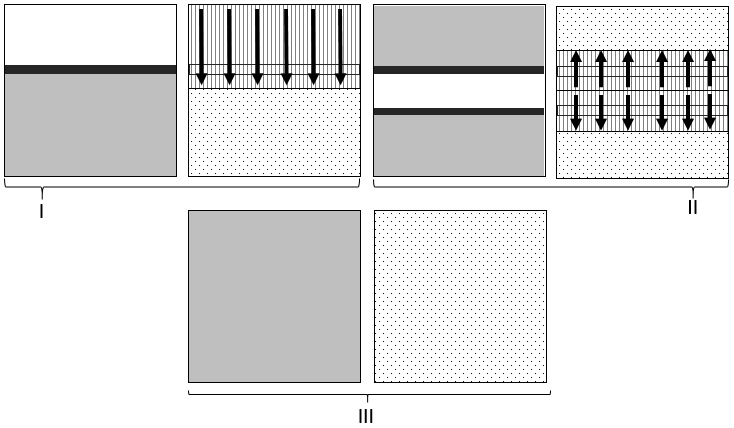
\includegraphics{img/fig-initial-states-nutrients.png}}
\end{center}\vspace*{-0.75cm}
\caption[Diagramas mostrando los esquemas de asignaci\'on de los estados iniciales con ejemplos de asignaci\'on de regiones y vectores de concentraci\'on de nutrientes]{Diagramas mostrando los esquemas de asignaci\'on de los estados iniciales con ejemplos de asignaci\'on de regiones y vectores de concentraci\'on de nutrientes. Posee la misma leyenda de colores de la figura~\ref{fig-initial-states-diagrams} para los diagramas izquierdos de cada par. Las regiones sombreadas con l\'ineas verticales poseen un vector de concentraci\'on de nutrientes con la direcci\'on especificada por la flecha, mientras que las regiones sombreadas con puntos indican una concentraci\'on uniforme de nutrientes. }
\label{fig-initial-states-nutrients}
\end{figure}

\section{Par\'ametros del modelo relacionados con la migraci\'on, invasi\'on y met\'astasis}
\label{subsec-model-param}
Los par\'ametros que se discuten en esta secci\'on se relacionan con las reglas y procedimientos de actualizaci\'on del aut\'omata celular encargados de reproducir los procesos de migraci\'on, invasi\'on y met\'astasis del c\'ancer. Se presentan en el cuadro~\ref{table-model-params} para una r\'apida referencia.

\begin{table}[!ht]
\begin{center}
\scalebox{0.9}{\begin{tabular}{|p{2cm}|p{14.5cm}|} \hline
\emph{Par\'ametro} & \emph{Descripci\'on} \\\hline
\multicolumn{1}{|c|}{$\mu_{mig}$} & Cantidad de movimientos tentativos que la c\'elula migratoria puede llevar a cabo en un instante de tiempo.\\\hline
\multicolumn{1}{|c|}{$\mu_{max}$} & Distancia m\'axima de migraci\'on.\\\hline
\multicolumn{1}{|c|}{$\xi_{sc}$} & Probabilidad de supervivencia de una c\'elula migratoria durante el transporte en el sistema circulatorio.\\\hline
\multicolumn{1}{|c|}{$\xi_{mic0}$,$\xi_{mic1}$} & Probabilidad de supervivencia de una micromet\'astasis.\\\hline
\multicolumn{1}{|c|}{$\psi_{mic0}$,$\psi_{mic1}$} & Probabilidad de colonizaci\'on de una micromet\'astasis.\\\hline
\multicolumn{1}{|c|}{$\eta_{mig}$} & Par\'ametro de ajuste de la probabilidad de transici\'on relacionada con la aparici\'on de c\'elulas migratorias.\\\hline
\multicolumn{1}{|c|}{$K_{mig}$} & Par\'ametro de ajuste de la probabilidad de transici\'on relacionada con la aparici\'on de c\'elulas migratorias.\\\hline
\multicolumn{1}{|c|}{$\eta_{mig}'$} & Par\'ametro de ajuste de la probabilidad de transici\'on relacionada con la muerte de c\'elulas migratorias durante su desplazamiento.\\\hline
\end{tabular}}\vspace*{-0.5cm}
\end{center}
\caption[Par\'ametros utilizados en el procedimiento de actualizaci\'on y en el ajuste de las reglas del aut\'omata celular]{Par\'ametros utilizados en el procedimiento de actualizaci\'on y en el ajuste de las reglas del aut\'omata celular.}
\label{table-model-params}
\end{table}

En~\cite{nurmenniemi} se expone que las c\'elulas migratorias de diversos tipos de carcinomas, entre los que se incluye el ductal infiltrante, son capaces de migrar desde la frontera del tumor hasta una distancia de $5$.$5 \times 10^{-1}mm$ en $14$ d\'ias como promedio. Si determinamos la velocidad de migraci\'on seg\'un los datos anteriores devuelve un promedio de $5$.$9 \times 10^{-2}mm$ en un d\'ia, valor cercano a las distancias entre c\'elulas del aut\'omata incluidas las diagonales que son de $3$.$5 \times 10^{-2}mm$ y $9$.$0 \times 10^{-2}mm$. Por tanto es razonable permitir en un lapso de $24$ horas que una c\'elula migratoria se desplace como m\'aximo una celda del aut\'omata en todas las direcciones, quedando el valor del par\'ametro $\mu_{mig} = 1$. Este par\'ametro es \'util si se desea ejecutar el aut\'omata celular con per\'iodos de tiempo diferentes para el crecimiento tumoral y para la migraci\'on; e.g. si el crecimiento tumoral se ejecuta con un per\'iodo de tiempo correspondiente con $24$ horas y la migraci\'on se eval\'ua con un per\'iodo de $48$ horas ser\'ia necesario hacer que $\mu_{mig} = 2$ para compensar. En~\cite{chaplain} se estima que la distancia m\'axima de migraci\'on de una c\'elula cancer\'igena est\'a entre $1mm$ y $10mm$. Dadas las dimensiones de una c\'elula en el aut\'omata, se pueden determinar la cantidad m\'axima de celdas que puede alejarse una c\'elula cancer\'igena de la frontera del tumor donde se originaron utilizando el dato anterior. Esto devuelve un valor entre $30$ y $300$ celdas aproximadamente, luego $\mu_{max} \in [30,300]$ con un valor promedio de $\mu_{max} = 165$ aproximadamente. De esta forma la cantidad de movimientos tentativos de una c\'elula se corresponden con la distancia m\'axima promedio de la migraci\'on siempre y cuando dicha c\'elula siempre se desplace en cada actualizaci\'on. 

En~\cite{luzzi} se estima experimentalmente que una c\'elula cancer\'igena solitaria que circule por el torrente sangu\'ineo tiene una probabilidad de supervivencia aproximada de $5$.$0 \times 10^{-4}$, mientras que en~\cite{aceto} se estima que los cl\'usteres de estas c\'elulas poseen una probabilidad de supervivencia entre $25$ y $50$ veces la supervivencia de una c\'elula solitaria, obteniendo un valor promedio de $1$.$9 \times 10^{-2}$. Dado que el presente modelo solo reproduce la migraci\'on de c\'elulas individuales se utiliza el valor de probabilidad de supervivencia determinado en~\cite{luzzi}, por tanto $\xi_{sc} = 5$.$0 \times 10^{-4}$. 

Seg\'un~\cite{kuhn,isogenic} los destinos m\'as frecuentes de las met\'astasis del carcinoma ductal infiltrante lo constituyen los huesos, pulmones e h\'igado en ese orden, en un $60\%$, $34\%$ y $20\%$ de los casos, mientras que las met\'astasis en la propia mama son muy poco frecuentes. Este hecho se puede interpretar de acuerdo a la teor\'ia de la semilla y el sustrato como un indicador de la hostilidad del entorno del \'organo hacia las c\'elulas cancer\'igenas, y por tanto puede utilizarse como v\'ia para determinar los par\'ametros $\xi_{mic}$ y $\psi_{mic}$. 

Como se expuso en la secci\'on~\ref{subsec-migrant}, la elecci\'on de los par\'ametros de ajuste $\eta_{mig}$ y $K_{mig}$ permite representar la aparici\'on de c\'elulas migratorias adecuadamente. En~\cite{kansal3} el valor de esta probabilidad de aparici\'on de c\'elulas migratorias se establece como un valor constante igual a $0$.$05$ en toda la simulaci\'on para obtener ramas invasivas poco densas, lo cual nos otorga una medida para ajustar nuestra funci\'on de probabilidad. Si se desea reproducir un c\'ancer con un alto nivel migratorio se precisa establecer un valor de probabilidad m\'as alto. En la gr\'afica~\ref{graph-probability-aparition} se muestran las distribuciones de probabilidad de la funci\'on $\rho_2(n_i \rightarrow 4)$~(\ref{eq-migrant-2}) que describe la aparici\'on de c\'elulas migratorias tanto en la frontera del tumor como en el interior del mismo para distintos par\'ametros. Estas gr\'aficas muestran que a medida que avanza el tiempo la probabilidad de que surjan c\'elulas migratorias se ve en aumento, tal y como ocurre con el proceso de acumulaci\'on de mutaciones. Mientras mayor es la cantidad de errores en el c\'odigo gen\'etico mayor es la agresividad de las c\'elulas cancer\'igenas, tomando la consideraci\'on de que las c\'elulas migratorias presentan una peligrosidad mayor que las c\'elulas que permanecen adheridas al tumor.

\begin{figure}[!ht]
\begin{center}
\subfigure[$K_{mig}=3$.$2 \times 10^{5}$]{\scalebox{0.88}{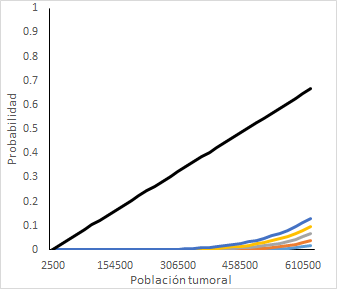
\includegraphics{img/graphs/graph-prob-aparition-1.png}}}
\subfigure[$K_{mig}=2$.$1 \times 10^{5}$]{\scalebox{0.88}{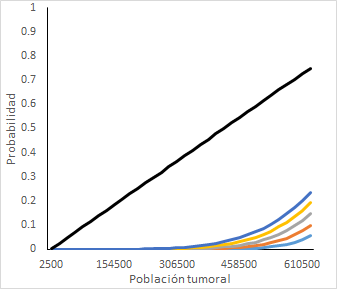
\includegraphics{img/graphs/graph-prob-aparition-2.png}}}
\subfigure[$K_{mig}=1$.$6 \times 10^{5}$]{\scalebox{0.88}{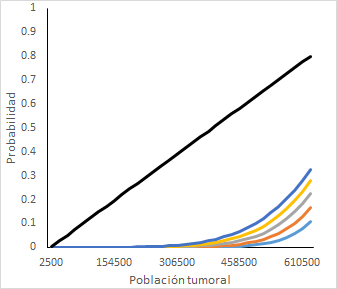
\includegraphics{img/graphs/graph-prob-aparition-3.png}}}
\subfigure[$K_{mig}=1$.$3 \times 10^{5}$]{\scalebox{0.88}{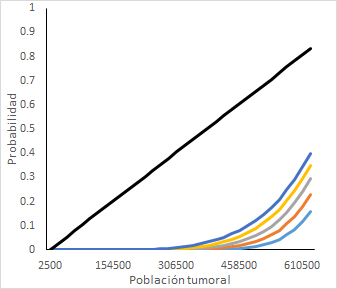
\includegraphics{img/graphs/graph-prob-aparition-4.png}}}
\end{center}\vspace*{-0.5cm}
\caption[Distribuciones de probabilidad de la funci\'on $\rho_2(n_i \rightarrow 4)$ que describe la aparici\'on de c\'elulas migratorias para distintos par\'ametros]{Distribuciones de probabilidad de la funci\'on $\rho_2(l \rightarrow 4)$ que describe la aparici\'on de c\'elulas migratorias. (a,b,c,d) En azul claro $\eta_{mig}=0$.$1$; en naranja $\eta_{mig}=0$.$125$; en gris $\eta_{mig}=0$.$15$; en amarillo $\eta_{mig}=0$.$175$; en azul oscuro $\eta_{mig}=0$.$2$; y en negro $\eta_{mig}=1$.}
\label{graph-probability-aparition}
\end{figure}

El par\'ametro de ajuste $\eta_{mig}'$ de la regla que determina la muerte de una c\'elula migratoria durante su avance por el estroma posee un funcionamiento similar a $\eta_{mig}$. En la gr\'afica~\ref{graph-probability-migration} se muestran las distribuciones de probabilidad de la funci\'on $\rho_4(\mu(v,n) \rightarrow 2)$~(\ref{eq-rho-4}) que describe la muerte de c\'elulas migratorias en su avance por el estroma. En estas gr\'aficas se muestra que una c\'elula migratoria a medida que permanece una mayor cantidad de tiempo en el estroma aumenta la probabilidad de que termine su existencia debido a su eliminaci\'on por parte del sistema inmunitario o de que ocurra por causas naturales como estr\'es mec\'anico, falta de nutrici\'on o por ausencia de se\~nales del entorno.

\begin{figure}[!ht]
\begin{center}
\subfigure[$\mu_{max}=150$]{\scalebox{0.88}{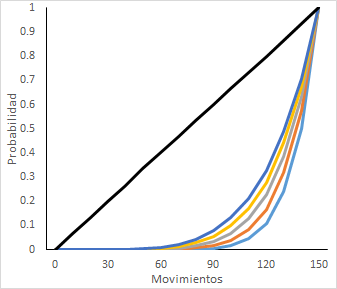
\includegraphics{img/graphs/graph-prob-migrant-1.png}}}
\subfigure[$\mu_{max}=300$]{\scalebox{0.88}{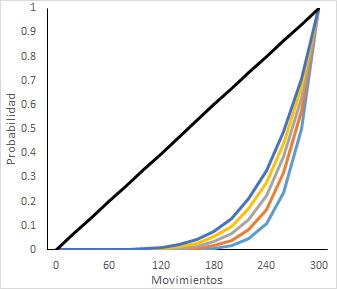
\includegraphics{img/graphs/graph-prob-migrant-2.png}}}
\end{center}\vspace*{-0.5cm}
\caption[Distribuciones de probabilidad de la funci\'on $\rho_4(\mu(v,n) \rightarrow 2)$ que describe la muerte de c\'elulas migratorias en su avance por el estroma para distintos par\'ametros]{Distribuciones de probabilidad de la funci\'on $\rho_4(\mu(v,n) \rightarrow 2)$ que describe la muerte de c\'elulas migratorias en su avance por el estroma para distintos par\'ametros. (a,b) En azul claro $\eta_{mig}'=0$.$1$; en naranja $\eta_{mig}'=0$.$125$; en gris $\eta_{mig}'=0$.$15$; en amarillo $\eta_{mig}'=0$.$175$; en azul oscuro $\eta_{mig}'=0$.$2$; y en verde $\eta_{mig}'=1$. }
\label{graph-probability-migration}
\end{figure}

\section{Escala de la simulaci\'on}
\label{subsec-scale-param}
En las secciones anteriores se ha descrito los procedimientos y an\'alisis que se llevan a cabo para obtener los par\'ametros del modelo necesarios para su ejecuci\'on. Estos par\'ametros se corresponden con una simulaci\'on en escala real, donde una c\'elula en la simulaci\'on equivale a una c\'elula en vida real. Una simulaci\'on de estas dimensiones puede tomar un lapso de tiempo enorme en concluir, haciendo que tareas como la obtenci\'on de datos estad\'isticos y validaci\'on del modelo presenten dificultades. Por tanto se opta por escalar los par\'ametros del modelo seg\'un el tama\~no de una celda del aut\'omata. En la escala real, o escala $1:1$, una celda del aut\'omata posee dimensiones $[0,3$.$5 \times 10^{-2}]mm \times [0, 3$.$5 \times 10^{-2}]mm$ correspondientes con el tama\~no aproximado que posee una c\'elula cancer\'igena de un carcinoma ductal infiltrante como se mostr\'o en la secci\'on~\ref{subsec-network-param}. La idea central es multiplicar el tama\~no de las celdas del aut\'omata por un valor de escala entero haciendo que cada celda del aut\'omata contenga una cantidad variable de c\'elulas reales, e.g. si se utiliza la escala $1:2$ las dimensiones de una celda del aut\'omata son $[0,7$.$0 \times 10^{-2}]mm \times [0, 7$.$0 \times 10^{-2}]mm$ correspondientes con $4$ c\'elulas reales. De esta forma el comportamiento de las c\'elulas reales contenidas en una misma celda se determina mediante una \'unica aplicaci\'on de las reglas del aut\'omata, reduciendo la cantidad de c\'alculos requeridos. 

Este procedimiento trae un problema relacionado con la representaci\'on de procesos como el crecimiento tumoral o la migraci\'on cancer\'igena. El m\'aximo incremento posible de la poblaci\'on de un tumor de un instante de tiempo $n$ a un instante $n+1$ lo constituyen las c\'elulas normales vecinas a la frontera del propio tumor. Dado que la influencia del estado de una c\'elula en sus vecinas est\'a limitada por el radio de la configuraci\'on de vecindad $R=\sqrt{2}$, como se expuso en la secci\'on~\ref{subsec-watts-2}, solo las c\'elulas normales que se sit\'uen a una distancia menor o igual a $R$ pueden ser desplazadas por el crecimiento tumoral. Esto se traduce en que un tumor representado por el aut\'omata puede incrementar su radio desde su centroide hasta la frontera exactamente la misma medida que posee una celda del mismo. Si se utiliza la escala $1:1$ en un lapso de $24$ horas el tumor puede incrementar cualquiera de sus radios en la medida de una celda, que en este caso se corresponde con la medida de una c\'elula real, es decir $3$.$5 \times 10^{-2}mm$. Pero en una escala mayor las celdas del aut\'omata poseen medidas mayores por lo que contienen una mayor cantidad de c\'elulas reales. Para lograr que los incrementos en el radio tumoral sean los correctos se debe incrementar el lapso de tiempo que ocurre entre instantes de tiempo y modificar adecuadamente los valores de $r$ y $\Delta t$. En la figura~\ref{fig-scales-1} se muestran ejemplos de varias escalas y el lapso de tiempo que se debe tomar para una representaci\'on adecuada. Se puede inferir que el lapso de tiempo se debe escalar la misma magnitud que las dimensiones de una celda del aut\'omata, e.g. si se utiliza la escala $1:2$ es necesario que el tiempo transcurrido entre los instantes $n$ y $n+1$ sea equivalente a $48$ horas que es el tiempo m\'inimo necesario para que una celda del aut\'omata sea ocupada por el tumor. Se asume que una celda del aut\'omata cuyo estado se corresponda con el de un tumor~(estado $3$) o el de una micromet\'astasis~(estado $4$) se encuentra totalmente ocupado por c\'elulas de esos tipos. N\'otese que este an\'alisis no posee contradicciones con lo expresado en la secci\'on~\ref{subsec-celldiv} sobre el sesgo direccional del crecimiento tumoral basado en la velocidad de expansi\'on.

\begin{figure}[!ht]
\begin{center}
\subfigure[Escala $1:1$]{\scalebox{0.67}{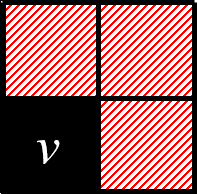
\includegraphics{img/fig-scales.png}}}
\subfigure[Escala $1:2$]{\scalebox{0.67}{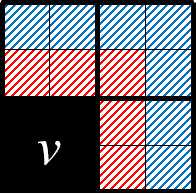
\includegraphics{img/fig-scales-1.png}}}
\subfigure[Escala $1:3$]{\scalebox{0.67}{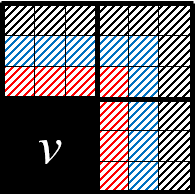
\includegraphics{img/fig-scales-2.png}}}
\end{center}\vspace*{-0.5cm}
\caption[Representaci\'on de distintas escalas del aut\'omata celular]{Representaci\'on de distintas escalas del aut\'omata celular y de los lapsos de tiempo necesarios para que un tumor se expanda satisfactoriamente a trav\'es del espacio mostrado. La celda $v$ representa una c\'elula tumoral que intenta expandirse a las celdas restantes. Las \'areas sombreadas muestran el tiempo m\'inimo necesario para que el tumor ocupe dichas c\'elulas seg\'un la escala utilizada. El color rojo se corresponde con $24$ horas, el color azul con $48$ horas y el negro con $72$ horas. (a) Las dimensiones de una celda del aut\'omata equivalen al de una c\'elula cancer\'igena $3$.$5 \times 10^{-2}mm$. (b) Las dimensiones de una celda del aut\'omata es el doble de una c\'elula cancer\'igena $7$.$0 \times 10^{-2}mm$ por lo que cada celda contiene $4$ c\'elulas. (c) Las dimensiones de una celda del aut\'omata es el triple de una c\'elula cancer\'igena $1$.$05 \times 10^{-1}mm$ por lo que cada celda contiene $9$ c\'elulas.}
\label{fig-scales-1}
\end{figure}

\begin{table}[!ht]
\begin{center}
\scalebox{1}{\begin{tabular}{|l|r|r|r|r|} \hline
\multicolumn{2}{|c|}{\emph{Par\'ametros}} & \multicolumn{3}{|c|}{\emph{Escalas}} \\\cline{3-5}
\multicolumn{2}{|c|}{} & \multicolumn{1}{|c|}{$1:1$} & \multicolumn{1}{|c|}{$1:2$} & \multicolumn{1}{|c|}{$1:3$} \\\hline
\emph{Dimensiones del espacio} & $s_x$ & $3000$ & $1500$ & $1000$ \\\cline{2-5}
                               & $s_y$ & $1500$ & $750$ & $500$ \\\hline
\multicolumn{2}{|l|}{\emph{Tiempo entre generaciones en horas}} & $24$ & $48$ & $72$ \\\hline
\multicolumn{2}{|l|}{\emph{C\'elulas contenidas en una celda}} & $1$ & $4$ & $9$ \\\hline

\emph{Poblaci\'on inicial avascular}& $P_0^a$ & $1$ & $1$ & $1$ \\\hline

\emph{Capacidad de carga avascular o}& $K_a$(m\'in) & $6$.$25 \times 10^2$ & $1$.$563 \times 10^2$ & $6$.$944 \times 10^1$ \\\cline{2-5}
\emph{poblaci\'on inicial vascular} & $K_a$(m\'ax) & $4$.$444 \times 10^3$ & $1$.$111 \times 10^3$ & $4$.$938 \times 10^2$ \\\cline{2-5}
									& $K_a$(med) & $2$.$535 \times 10^3$ & $4$.$592 \times 10^2$ & $2$.$222 \times 10^2$ \\\hline

\emph{Capacidad de carga vascular} & $K_v$(m\'in) & $2$.$5 \times 10^5$ & $6$.$25 \times 10^4$ & $2$.$778 \times 10^4$ \\\cline{2-5}
                                   & $K_v$(m\'ax) & $1$.$0 \times 10^6$ & $2$.$5 \times 10^5$ & $1$.$111 \times 10^5$ \\\cline{2-5}
                                   & $K_v$(med) & $6$.$25 \times 10^5$ & $1$.$276 \times 10^5$ & $5$.$556 \times 10^4$ \\\hline

\emph{Movimientos tentativos} & $\mu_{mig}$ & $1$ & $1$ & $1$\\\hline

\emph{Distancia m\'axima de la migraci\'on} & $\mu_{max}$ & $165$ & $84$ & $55$ \\\hline
\end{tabular}}\vspace*{-0.5cm}
\end{center}
\caption[Escalas consideradas para su utilizaci\'on en el aut\'omata celular]{Escalas consideradas para su utilizaci\'on en el aut\'omata celular. Se muestran varios par\'ametros del modelo corregidos para dichas escalas.}
\label{table-reescale}
\end{table} 

El an\'alisis seguido para el crecimiento tumoral se puede realizar de igual forma con la migraci\'on, obteni\'endose la misma conclusi\'on. En la secci\'on~\ref{subsec-model-param} se expuso que una c\'elula migratoria puede desplazarse aproximadamente $3$.$9 \times 10^{-2}mm$ en $24$ horas, que se corresponde con una celda del aut\'omata en la escala real. Si utilizamos un tama\~no mayor para las celdas del aut\'omata una c\'elula migratoria deber\'a tomarle m\'as tiempo para avanzar desde una celda hacia la siguiente. Luego el lapso de tiempo transcurrido entre los instantes de tiempo $n$ y $n+1$ debe aumentar para reproducir de forma adecuada dicho movimiento. 

El otro problema que presenta el uso de escalas gira en torno a las cantidades de c\'elulas cancer\'igenas que penetran el torrente sangu\'ineo, ya sea como la culminaci\'on de la migraci\'on o que esta penetraci\'on ocurra desde el interior del propio tumor. En escala real la migraci\'on y la penetraci\'on del torrente sangu\'ineo desde los capilares del tumor se lleva a cabo por c\'elulas individuales, pero si se utiliza una escala se establece que el comportamiento de varias c\'elulas se determina mediante la aplicaci\'on de una misma regla. Para el crecimiento tumoral se asume que la cantidad de c\'elulas contenidas en una celda del aut\'omata se corresponde con la cantidad m\'axima que puede contener. Esta suposici\'on se sostiene en el hecho que el interior del tumor contin\'ua desarroll\'andose cubriendo los espacios existentes. Con respecto a las c\'elulas migratorias se asigna un valor entero aleatorio perteneciente al intervalo $[1,max]$ a cada c\'elula que surge de este tipo, correspondiente con la cantidad de c\'elulas contenidas en dicha celda del aut\'omata, donde $max$ es la m\'axima cantidad de c\'elulas que puede contener una celda, e.g en la escala $1:2$ el valor de $max=4$. Este mecanismo se implementa de forma similar en el algoritmo encargado de reproducir la intravasaci\'on desde el interior del tumor de c\'elulas migratorias. En el cuadro~\ref{table-reescale} se muestran varios par\'ametros del modelo de aut\'omatas que se han obtenido en las secciones anteriores corregidos para su utilizaci\'on con las escalas consideradas. Despu\'es de sucesivas pruebas se descarta la posibilidad de utilizar las escalas $1:1$ y $1:2$ debido a la carga computacional que presentan. 

\newpage
\chapter{Resultados computacionales}
\label{sec-results}
Los par\'ametros obtenidos en la secci\'on anterior~\ref{sec-validation} permiten ejecutar el aut\'omata celular concebido para la reproducci\'on del ciclo vital del c\'ancer. Los resultados que se presentan en esta secci\'on se obtuvieron promediando los datos provenientes de la ejecuci\'on de varias simulaciones del aut\'omata, preferiblemente un m\'inimo de $30$ simulaciones. En esta tarea se utiliz\'o un ordenador personal de gama baja-media con un procesador Intel Core $i3$ compuesto por $4$ n\'ucleos a una frecuencia de reloj de $2$.$2\,GHz$ y $8\,GB$ de memoria de acceso aleatorio ($RAM$). Se procede explorando en las secciones correspondientes~\ref{sec-avascular-results}--\ref{sec-metastasis-validation} los distintos comportamientos y etapas que presenta el c\'ancer, presentando los par\'ametros del modelo utilizados, la influencia de la variaci\'on de los mismos y las similitudes con los datos provenientes de otras investigaciones citadas respectivamente. En la secci\'on~\ref{subsec-scale-param} se expuso que la escala utilizada en la ejecuci\'on del aut\'omata es $1:3$. En cuanto a la asignaci\'on de los estados iniciales se utiliza el esquema I para el \'organo primario correspondiente con la mama, y el esquema III para el \'organo secundario correspondiente con los huesos como se mostr\'o en la secci\'on~\ref{subsec-states-param}, que en el caso del carcinoma ductal infiltrante constituye el destino m\'as frecuente de las met\'astasis. Partimos mostrando los par\'ametros de la construcci\'on de la red, de la asignaci\'on de estados iniciales y de las regiones y vectores de nutrientes en el cuadro~\ref{table-net-params}. 

\begin{table}[!ht]
\begin{center}
\scalebox{0.9}{\begin{tabular}{|p{2cm}|p{14.5cm}|}\hline
\emph{Red} & $s_x=1000$; $s_y=500$; $s_o=500$; $p = 0$.$01$. \\\hline

\emph{Estados} & Para el \'organo primario correspondiente con la mama -- Esquema I: $o_l=250$, $o_e=1$, $o_s=249$, $v_x^t=250$, $v_y^t=250$. Para el \'organo secundario correspondiente con los huesos -- Esquema III: $o_s=500$.\\\hline 

\emph{Nutrientes} & Para el \'organo primario -- $R_1 = \lbrace v~|~v \in V(G) : (0 \leq v_x < 500) \wedge (0 \leq v_y < 276) \rbrace$, $B_{01}=\lbrace \overrightarrow{\nu_{((0,0),(0,1))}} \rbrace$, $R_2 = \lbrace v~|~v \in V(G) : (0 \leq v_x < 500) \wedge (276 \leq v_y < 500) \rbrace$. Para el \'organo secundario -- $R_3 = \lbrace v~|~v \in V(G) : (500 \leq v_x < 1000) \wedge (0 \leq v_y < 500) \rbrace$.\\\hline
\end{tabular}}\vspace*{-0.5cm}
\end{center}
\caption[Valores de los par\'ametros de construcci\'on de la red, de la asignaci\'on de estados iniciales y de las regiones y vectores de nutrientes]{Valores de los par\'ametros de construcci\'on de la red, de la asignaci\'on de estados iniciales y de las regiones y vectores de nutrientes. Se utiliza la escala $1:3$ donde el tiempo transcurrido entre las generaciones del aut\'omata $n$ y $n+1$ se corresponde a $72$ horas y cada celda del aut\'omata contiene $9$ c\'elulas reales.}
\label{table-net-params}
\end{table}

\section{Crecimiento avascular}
\label{sec-avascular-results}
El primer conjunto de par\'ametros de la ley de crecimiento log\'istica, mostrada en las expresiones~(\ref{eq-pa}) y~(\ref{eq-pv}), describen el desarrollo de un tumor avascular de crecimiento r\'apido. Para ello se utilizan los valores de la poblaci\'on inicial y de las capacidades de carga m\'inimas, promedio y m\'aximas correspondientes con el intervalo de radios avasculares $R_a \in [0$.$5, 1]mm$ y una probabilidad m\'axima avascular $\rho_{max}^a=1$ como se muestran en el cuadro~\ref{table-avascular}. Los resultados provenientes de las simulaciones con los par\'ametros del cuadro~\ref{table-avascular} se muestran en las gr\'aficas~\ref{graph-avascular-simulations}. El an\'alisis de los resultados presentados se lleva a cabo en la secci\'on~\ref{sec-growth-validation}.
\begin{table}[!ht]
\begin{center}
\scalebox{0.9}{\begin{tabular}{|p{2.1cm}|p{14.5cm}|}\hline
\emph{M\'inimo} & $P_0^a=1$, $K_a=6$.$944 \times 10^1$, $r_a=5$.$797 \times 10^{-2}$, $\Delta t=1$.$693 \times 10^1$, $n_a=9$, generaciones del aut\'omata: $10$~($30$ d\'ias). \\\hline
\emph{Promedio} & $P_0^a=1$, $K_a=2$.$222 \times 10^2$, $r_a=1$.$802 \times 10^{-2}$, $\Delta t=2$.$996 \times 10^1$, $n_a=20$, generaciones del aut\'omata: $21$~($63$ d\'ias).\\\hline
\emph{M\'aximo} & $P_0^a=1$, $K_a=4$.$938 \times 10^2$, $r_a=8$.$097 \times 10^{-3}$, $\Delta t=4$.$558 \times 10^1$, $n_a=34$, generaciones del aut\'omata: $35$~($105$ d\'ias).\\\hline
\end{tabular}}\vspace*{-0.6cm}
\end{center}
\caption[Par\'ametros del desarrollo de un carcinoma ductal infiltrante de crecimiento r\'apido durante la etapa avascular]{Par\'ametros del desarrollo de un carcinoma ductal infiltrante de crecimiento r\'apido durante la etapa avascular.}
\label{table-avascular}
\end{table}

\begin{figure}[p]
\begin{center}
\subfigure[Crecimiento m\'inimo $K_a=6$.$944 \times 10^1$]{\scalebox{0.8}{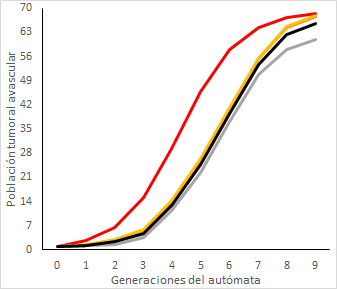
\includegraphics{img/graphs/graph-avascular-simulations-min.png}}
\scalebox{0.8}{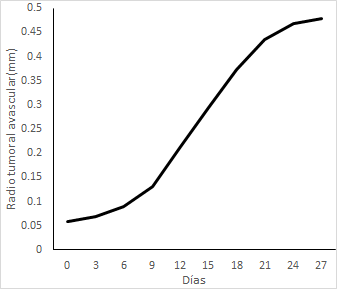
\includegraphics{img/graphs/graph-avascular-simulations-min-r.png}}}\vspace*{-0.2cm}
\subfigure[Crecimiento promedio $K_a=2$.$222 \times 10^2$]{\scalebox{0.8}{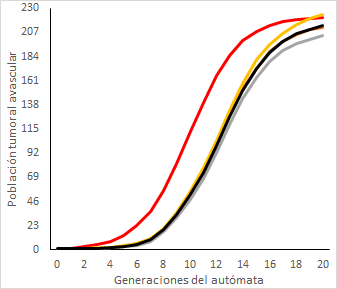
\includegraphics{img/graphs/graph-avascular-simulations-pro.png}}
\scalebox{0.8}{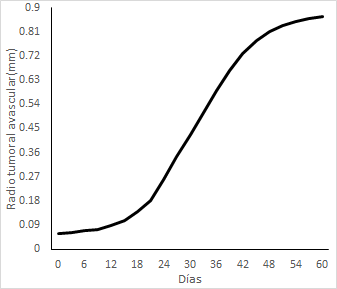
\includegraphics{img/graphs/graph-avascular-simulations-pro-r.png}}}\vspace*{-0.2cm}
\subfigure[Crecimiento m\'aximo $K_a=4$.$938 \times 10^2$]{\scalebox{0.8}{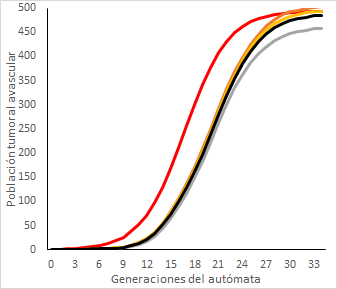
\includegraphics{img/graphs/graph-avascular-simulations-max.png}}
\scalebox{0.8}{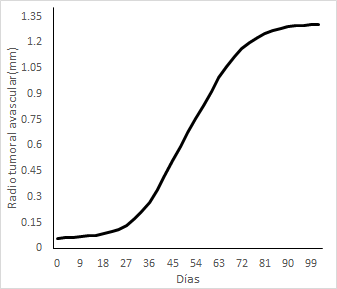
\includegraphics{img/graphs/graph-avascular-simulations-max-r.png}}}\vspace*{-0.2cm}
\end{center}\vspace*{-0.6cm}
\caption[Poblaci\'on y radios de un carcinoma ductal infiltrante de crecimiento r\'apido con $\rho_{max}^a=1$ durante la etapa avascular]{Poblaci\'on y radios de un carcinoma ductal infiltrante de crecimiento r\'apido con $\rho_{max}^a=1$ durante la etapa avascular. El resto de par\'ametros se muestran en el cuadro~\ref{table-avascular}. (a,b,c--izquierda) En rojo los valores obtenidos de la soluci\'on de la ley de crecimiento log\'istico, en negro los promedios de la poblaci\'on tumoral y el resto de curvas son varias simulaciones del aut\'omata. (a,b,c--derecha) En negro los promedios del radio tumoral.}
\label{graph-avascular-simulations}
\end{figure}

Con el objetivo de establecer comparaciones se determina un conjunto de par\'ametros del modelo de crecimiento log\'istico que describen el desarrollo de un tumor avascular de crecimiento lento. Para ello se utilizan los valores de la poblaci\'on inicial y de las capacidades de carga m\'inimas, promedio y m\'aximas correspondientes con el intervalo de radios avasculares $R_a \in [0$.$5, 1]mm$ y una probabilidad m\'axima avascular $\rho_{max}^a=0$.$1$ como se muestra en el cuadro~\ref{table-avascular-1}. El modelo puede reproducir tumores que toman mucho m\'as tiempo para su desarrollo pero se considera adecuado mostrar el crecimiento para la anterior probabilidad m\'axima $\rho_{max}^a=0$.$1$ para establecer dichas comparaciones; e.g. tumores con una probabilidad m\'axima menor como $\rho_{max}^a=0$.$01$. Los resultados provenientes de las simulaciones con los par\'ametros del cuadro~\ref{table-avascular-1} se muestran en las gr\'aficas~\ref{graph-avascular-simulations-1}. El an\'alisis de los resultados presentados se lleva a cabo en la secci\'on~\ref{sec-growth-validation}.
\begin{table}[!ht]
\begin{center}
\scalebox{0.9}{\begin{tabular}{|p{2.1cm}|p{14.5cm}|}\hline
\emph{M\'inimo} & $P_0^a=1$, $K_a=6$.$944 \times 10^1$, $r_a=5$.$797 \times 10^{-3}$, $\Delta t=2$.$854 \times 10^1$, $n_a=51$, generaciones del aut\'omata: $52$~($156$ d\'ias).\\\hline
\emph{Promedio} & $P_0^a=1$, $K_a=2$.$222 \times 10^2$, $r_a=1$.$802 \times 10^{-3}$, $\Delta t=5$.$497 \times 10^1$, $n_a=109$, generaciones del aut\'omata: $110$~($330$ d\'ias).\\\hline
\emph{M\'aximo} & $P_0^a=1$, $K_a=4$.$938 \times 10^2$, $r_a=8$.$097 \times 10^{-4}$, $\Delta t=8$.$604 \times 10^1$, $n_a=178$, generaciones del aut\'omata: $179$~($537$ d\'ias).\\\hline
\end{tabular}}\vspace*{-0.6cm}
\end{center}
\caption[Par\'ametros del desarrollo de un carcinoma ductal infiltrante de crecimiento lento durante la etapa avascular]{Par\'ametros del desarrollo de un carcinoma ductal infiltrante de crecimiento lento durante la etapa avascular.}
\label{table-avascular-1}
\end{table}

\begin{figure}[p]
\begin{center}
\subfigure[Crecimiento m\'inimo $K_a=6$.$944 \times 10^1$]{\scalebox{0.8}{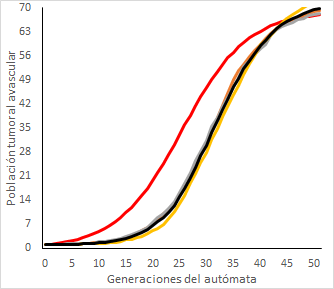
\includegraphics{img/graphs/graph-avascular-simulations-min-1.png}}
\scalebox{0.8}{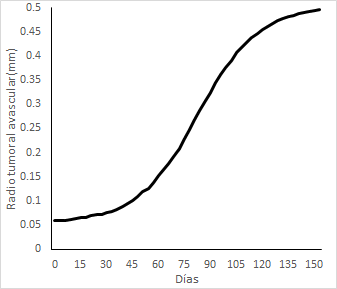
\includegraphics{img/graphs/graph-avascular-simulations-min-r-1.png}}}\vspace*{-0.2cm}
\subfigure[Crecimiento promedio $K_a=2$.$222 \times 10^2$]{\scalebox{0.8}{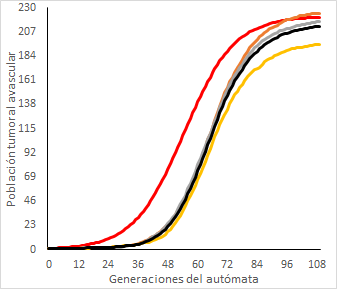
\includegraphics{img/graphs/graph-avascular-simulations-pro-1.png}}
\scalebox{0.8}{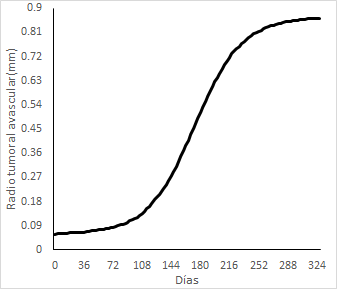
\includegraphics{img/graphs/graph-avascular-simulations-pro-r-1.png}}}\vspace*{-0.2cm}
\subfigure[Crecimiento m\'aximo $K_a=4$.$938 \times 10^2$]{\scalebox{0.8}{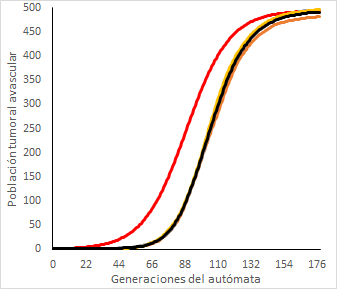
\includegraphics{img/graphs/graph-avascular-simulations-max-1.png}}
\scalebox{0.8}{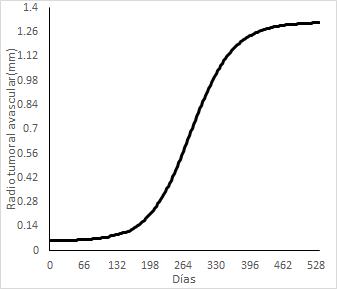
\includegraphics{img/graphs/graph-avascular-simulations-max-r-1.png}}}\vspace*{-0.2cm}
\end{center}\vspace*{-0.6cm}
\caption[Poblaci\'on y radios de un carcinoma ductal infiltrante de crecimiento lento con $\rho_{max}^a=0$.$1$ durante la etapa avascular]{Poblaci\'on y radios de un carcinoma ductal infiltrante de crecimiento lento con $\rho_{max}^a=0$.$1$ durante la etapa avascular. El resto de par\'ametros se muestran en el cuadro~\ref{table-avascular-1}. (a,b,c--izquierda) En rojo los valores obtenidos de la soluci\'on de la ley de crecimiento log\'istico, en negro los promedios de la poblaci\'on tumoral y el resto de curvas son varias simulaciones del aut\'omata. (a,b,c--derecha) En negro los promedios del radio tumoral.}
\label{graph-avascular-simulations-1}
\end{figure}

En la figura~\ref{fig-avascular-automata} se muestran las visualizaciones de una de las simulaciones del aut\'omata de un carcinoma ductal infiltrante de crecimiento r\'apido durante la etapa avascular. Al tratarse de un carcinoma que constituye un tipo de c\'ancer que surge en el epitelio~(en naranja) se puede apreciar que comienza su desarrollo en esta capa de tejido. Se puede apreciar, adem\'as, la adecuada aplicaci\'on de la regla del crecimiento tumoral definida en la secci\'on~\ref{subsec-celldiv} que establece que durante la etapa avascular un tumor primario no puede penetrar la membrana basal e invadir el estroma~(en gris). En ninguna de las im\'agenes se evidencia esta invasi\'on. La influencia de los vectores de concentraci\'on de nutrientes definen la direcci\'on de la expansi\'on tumoral~(en negro) que se mantiene paralela al epitelio y avanza de forma limitada hacia el lumen~(en blanco). La invasi\'on del estroma tiene lugar durante la etapa vascular del tumor primario y durante las etapas avascular y vascular en tumores secundarios. 
\begin{figure}[!ht]
\begin{center}
\subfigure[Generaci\'on 0]{\scalebox{0.29}{\includegraphics{img/automata/2019519191641-0.png}}}
\subfigure[Generaci\'on 4]{\scalebox{0.29}{\includegraphics{img/automata/2019519191641-4.png}}}
\subfigure[Generaci\'on 8]{\scalebox{0.29}{\includegraphics{img/automata/2019519191641-8.png}}}\vspace*{-0.25cm}
\subfigure[Generaci\'on 12]{\scalebox{0.29}{\includegraphics{img/automata/2019519191641-12.png}}}
\subfigure[Generaci\'on 16]{\scalebox{0.29}{\includegraphics{img/automata/2019519191641-16.png}}}
\subfigure[Generaci\'on 20]{\scalebox{0.29}{\includegraphics{img/automata/2019519191641-20.png}}}\vspace*{-0.25cm}
\end{center}\vspace*{-0.6cm}
\caption[Visualizaciones de una simulaci\'on del aut\'omata celular de un carcinoma ductal infiltrante de crecimiento r\'apido durante la etapa avascular]{Visualizaciones de una simulaci\'on del aut\'omata celular de un carcinoma ductal infiltrante de crecimiento r\'apido durante la etapa avascular. Las generaciones del aut\'omata mostradas se obtienen mediante los par\'ametros correspondientes con la capacidad de carga promedio~(cuadro~\ref{table-avascular}). El \'area mostrada posee dimensiones $[0,10$.$5]mm \times [0,10$.$5]mm$.}
\label{fig-avascular-automata}
\end{figure}

\section{Crecimiento vascular}
\label{sec-vascular-results}
Este conjunto de par\'ametros de la ley de crecimiento log\'istica describen el desarrollo de un tumor vascular de crecimiento r\'apido. Para ello se utilizan los valores de la poblaci\'on inicial y de las capacidades de carga m\'inimas, promedio y m\'aximas correspondientes con el intervalo de radios vasculares $R_v \in [10, 15]mm$ y una probabilidad m\'axima vascular $\rho_{max}^v=1$ como se muestra en el cuadro~\ref{table-vascular}. La poblaci\'on inicial utilizada es la capacidad de carga avascular promedio, es decir, $P_0^v = K_a = 2$.$222 \times 10^2$. Los resultados provenientes de las simulaciones con los par\'ametros del cuadro~\ref{table-vascular} se muestran en las gr\'aficas~\ref{graph-vascular-simulations}. El an\'alisis de los resultados presentados se lleva a cabo en la secci\'on~\ref{sec-growth-validation}.
\begin{table}[!ht]
\begin{center}
\scalebox{0.9}{\begin{tabular}{|p{2.1cm}|p{14.5cm}|}\hline
\emph{M\'inimo} & $P_0^v=2$.$222 \times 10^2$, $K_v=2$.$778 \times 10^4$, $r_v=1$.$44 \times 10^{-4}$, $\Delta t=5$.$401 \times 10^2$, generaciones del aut\'omata: $121$~($363$ d\'ias).\\\hline
\emph{Promedio} & $P_0^v=2$.$222 \times 10^2$, $K_v=5$.$556 \times 10^4$, $r_v=7$.$199 \times 10^{-5}$, $\Delta t=7$.$665 \times 10^2$, generaciones del aut\'omata: $201$~($603$ d\'ias).\\\hline
\emph{M\'aximo} & $P_0^v=2$.$222 \times 10^2$, $K_v=1$.$111 \times 10^5$, $r_v=3$.$6 \times 10^{-5}$, $\Delta t=1$.$079 \times 10^3$, generaciones del aut\'omata: $321$~($963$ d\'ias).\\\hline
\end{tabular}}\vspace*{-0.6cm}
\end{center}
\caption[Par\'ametros del desarrollo de un carcinoma ductal infiltrante de crecimiento r\'apido durante la etapa vascular]{Par\'ametros del desarrollo de un carcinoma ductal infiltrante de crecimiento r\'apido durante la etapa vascular.}
\label{table-vascular}
\end{table}

\begin{figure}[p]
\begin{center}
\subfigure[Crecimiento m\'inimo $K_v=2$.$778 \times 10^4$]{\scalebox{0.8}{\includegraphics{img/graphs/graph-vascular-simulations-min.png}}
\scalebox{0.8}{\includegraphics{img/graphs/graph-vascular-simulations-min-r.png}}}\vspace*{-0.2cm}
\subfigure[Crecimiento promedio $K_v=5$.$556 \times 10^4$]{\scalebox{0.8}{\includegraphics{img/graphs/graph-vascular-simulations-pro.png}}
\scalebox{0.8}{\includegraphics{img/graphs/graph-vascular-simulations-pro-r.png}}}\vspace*{-0.2cm}
\subfigure[Crecimiento m\'aximo $K_v=1$.$111 \times 10^5$]{\scalebox{0.8}{\includegraphics{img/graphs/graph-vascular-simulations-max.png}}
\scalebox{0.8}{\includegraphics{img/graphs/graph-vascular-simulations-max-r.png}}}\vspace*{-0.2cm}
\end{center}\vspace*{-0.6cm}
\caption[Poblaci\'on y radios de un carcinoma ductal infiltrante de crecimiento r\'apido con $\rho_{max}^v=1$ durante la etapa vascular]{Poblaci\'on y radios de un carcinoma ductal infiltrante de crecimiento r\'apido con $\rho_{max}^v=1$ durante la etapa vascular. El resto de par\'ametros se muestran en el cuadro~\ref{table-vascular}. (a,b,c--izquierda) En rojo los valores obtenidos de la soluci\'on de la ley de crecimiento log\'istico, en negro los promedios de la poblaci\'on tumoral y el resto de curvas son varias simulaciones del aut\'omata. (a,b,c--derecha) En negro los promedios del radio tumoral.}
\label{graph-vascular-simulations}
\end{figure}

\begin{figure}[p]
\begin{center}
\subfigure[Crecimiento m\'inimo $K_v=2$.$778 \times 10^4$]{\scalebox{0.8}{\includegraphics{img/graphs/graph-vascular-simulations-min-1.png}}
\scalebox{0.8}{\includegraphics{img/graphs/graph-vascular-simulations-min-r-1.png}}}\vspace*{-0.2cm}
\subfigure[Crecimiento promedio $K_v=5$.$556 \times 10^4$]{\scalebox{0.8}{\includegraphics{img/graphs/graph-vascular-simulations-pro-1.png}}
\scalebox{0.8}{\includegraphics{img/graphs/graph-vascular-simulations-pro-r-1.png}}}\vspace*{-0.2cm}
\subfigure[Crecimiento m\'aximo $K_v=1$.$111 \times 10^5$]{\scalebox{0.8}{\includegraphics{img/graphs/graph-vascular-simulations-max-1.png}}
\scalebox{0.8}{\includegraphics{img/graphs/graph-vascular-simulations-max-r-1.png}}}\vspace*{-0.2cm}
\end{center}\vspace*{-0.6cm}
\caption[Poblaci\'on y radios de un carcinoma ductal infiltrante de crecimiento lento con $\rho_{max}^v=0$.$1$ durante la etapa vascular]{Poblaci\'on y radios de un carcinoma ductal infiltrante de crecimiento lento con $\rho_{max}^v=0$.$1$ durante la etapa vascular. El resto de par\'ametros se muestran en el cuadro~\ref{table-vascular-1}. (a,b,c--izquierda) En rojo los valores obtenidos de la soluci\'on de la ley de crecimiento log\'istico, en negro los promedios de la poblaci\'on tumoral y el resto de curvas son varias simulaciones del aut\'omata. (a,b,c--derecha) En negro los promedios del radio tumoral.}
\label{graph-vascular-simulations-1}
\end{figure}

Con el objetivo de establecer comparaciones se determina un conjunto de par\'ametros del modelo de crecimiento log\'istico que describen el desarrollo de un tumor vascular de crecimiento lento. Para ello se utilizan los valores de la poblaci\'on inicial y de las capacidades de carga m\'inimas, promedio y m\'aximas correspondientes con el intervalo de radios vasculares $R_v \in [10, 15]mm$ y una probabilidad m\'axima avascular $\rho_{max}^v=0$.$1$ como se muestra en el cuadro~\ref{table-vascular-1}. El modelo puede reproducir tumores que toman mucho m\'as tiempo para su desarrollo pero se considera adecuado mostrar el crecimiento para la anterior probabilidad m\'axima $\rho_{max}^v=0$.$1$ para establecer dichas comparaciones; e.g. tumores con una probabilidad m\'axima menor como $\rho_{max}^v=0$.$01$. Los resultados provenientes de las simulaciones con los par\'ametros del cuadro~\ref{table-vascular-1} se muestran en las gr\'aficas~\ref{graph-vascular-simulations-1}. El an\'alisis de los resultados presentados se lleva a cabo en la secci\'on~\ref{sec-growth-validation}.
\begin{table}[!ht]
\begin{center}
\scalebox{0.9}{\begin{tabular}{|p{2.1cm}|p{14.5cm}|}\hline
\emph{M\'inimo} & $P_0^v=2$.$222 \times 10^2$, $K_v=2$.$778 \times 10^4$, $r_v=1$.$44 \times 10^{-5}$, $\Delta t=1$.$187 \times 10^3$, generaciones del aut\'omata: $565$~($1695$ d\'ias).\\\hline
\emph{Promedio} & $P_0^v=2$.$222 \times 10^2$, $K_v=5$.$556 \times 10^4$, $r_v=7$.$199 \times 10^{-6}$, $\Delta t=1$.$659 \times 10^3$, generaciones del aut\'omata: $925$~($2775$ d\'ias).\\\hline
\emph{M\'aximo} & $P_0^v=2$.$222 \times 10^2$, $K_v=1$.$111 \times 10^5$, $r_v=8$.$097 \times 10^{-3}$, $\Delta t=4$.$558 \times 10^1$, generaciones del aut\'omata: $1481$~($4443$ d\'ias).\\\hline
\end{tabular}}\vspace*{-0.6cm}
\end{center}
\caption[Par\'ametros del desarrollo de un carcinoma ductal infiltrante de crecimiento lento durante la etapa vascular]{Par\'ametros del desarrollo de un carcinoma ductal infiltrante de crecimiento lento durante la etapa vascular.}
\label{table-vascular-1}
\end{table}

En la figura~\ref{fig-vascular-automata} se muestran las visualizaciones de una de las simulaciones del aut\'omata de un tumor vascular de crecimiento r\'apido. En estas visualizaciones no se muestran poblaciones de c\'elulas migratorias ni de micromet\'astasis porque estas reglas no fueron evaluadas durante estas simulaciones con el objetivo de mostrar solamente el crecimiento vascular del tumor. Se puede apreciar un aumento considerable de la poblaci\'on tumoral, as\'i como la invasi\'on del estroma que avanza progresivamente a medida que avanza su desarrollo. En las gr\'aficas para el crecimiento vascular no es posible apreciar correctamente las curvas correspondientes con varias simulaciones del aut\'omata pues son en extremo cercanas a la curva que representa el promedio.
\begin{figure}[!ht]
\begin{center}
\subfigure[Generaci\'on 0]{\scalebox{0.29}{\includegraphics{img/automata/201951822631-22.png}}}
\subfigure[Generaci\'on 40]{\scalebox{0.29}{\includegraphics{img/automata/201951822631-62.png}}}
\subfigure[Generaci\'on 80]{\scalebox{0.29}{\includegraphics{img/automata/201951822631-102.png}}}\vspace*{-0.25cm}
\subfigure[Generaci\'on 120]{\scalebox{0.29}{\includegraphics{img/automata/201951822631-142.png}}}
\subfigure[Generaci\'on 160]{\scalebox{0.29}{\includegraphics{img/automata/201951822631-182.png}}}
\subfigure[Generaci\'on 200]{\scalebox{0.29}{\includegraphics{img/automata/201951822631-221.png}}}\vspace*{-0.25cm}
\end{center}\vspace*{-0.6cm}
\caption[Visualizaciones de una simulaci\'on del aut\'omata celular de un carcinoma ductal infiltrante de crecimiento r\'apido durante la etapa vascular]{Visualizaciones de una simulaci\'on del aut\'omata celular de un carcinoma ductal infiltrante de crecimiento r\'apido durante la etapa vascular. Las generaciones del aut\'omata mostradas se obtienen mediante los par\'ametros correspondientes con la capacidad de carga promedio~(cuadro~\ref{table-vascular}) y se toman relativas al inicio de dicha etapa. El \'area mostrada posee dimensiones $[0,52$.$5]mm \times [0,52$.$5]mm$.}
\label{fig-vascular-automata}
\end{figure}

\section{Validaci\'on del crecimiento tumoral}
\label{sec-growth-validation}
Como se pudo apreciar en los datos obtenidos de la simulaci\'on del crecimiento tumoral durante las etapas avascular y vascular la curva descrita por la utilizaci\'on de la ecuaci\'on de crecimiento log\'istica posee la forma caracter\'istica de \emph{S}~\cite{book} presente en otros modelos de la literatura que utilizan otras ecuaciones de crecimiento como Gompertz~\cite{kansal,dormann,kansal2,kansal3}, en las que el crecimiento se divide en tres etapas representativas: una fase inicial pasiva, una fase intermedia de crecimiento exponencial y una fase final de ralentizaci\'on. Estas tres etapas se evidencian claramente en las gr\'aficas~\ref{graph-avascular-simulations}, \ref{graph-avascular-simulations-1}, \ref{graph-vascular-simulations} y \ref{graph-vascular-simulations-1} provenientes de las simulaciones computacionales del modelo. Las ejecuciones del aut\'omata celular reproducen el crecimiento log\'istico con diferencias causadas principalmente por la naturaleza desigual de ambos modelos. Las causas que se listan a continuaci\'on se aplican a las diferencias entre la ley de crecimiento log\'istico y el modelo de aut\'omatas celulares concebido tanto durante la etapa avascular como durante la vascular: la influencia de los vectores de concentraci\'on~($\beta_{tum}(v,l)$), la influencia de la velocidad de expansi\'on~($\gamma_{tum}(v,N(v,l))$) y el error de aproximaci\'on proveniente del uso de la escala $1:3$.

Durante la realizaci\'on de las simulaciones computacionales se comprob\'o que el modelo devuelve valores biol\'ogicamente realistas, tanto en el tiempo como en las cantidades de c\'elulas cancer\'igenas presentes en ambas etapas del crecimiento. En cuanto al tiempo el $50\%$ de los casos de carcinomas se consideran tumores de crecimiento r\'apido y se desarrollan en un lapso de $1$--$2$ a\~nos, el $33\%$ de los casos se consideran tumores de crecimiento intermedio y se desarrollan en un lapso de $2$--$5$ a\~nos, y cerca del $17\%$ de los casos se consideran tumores de crecimiento lento desarroll\'andose todo el ciclo tumoral en un lapso mayor de $5$ a\~nos pr\'acticamente sin l\'imite de tiempo~\cite{nakashima,leekim,sopik}. Los casos extremos mostrados anteriormente para ambas etapas demuestran que el modelo es capaz de reconstruir el desarrollo tumoral para un per\'iodo de tiempo arbitrario; e.g. si se desea reproducir el desarrollo de un tumor de crecimiento r\'apido se pueden combinar los par\'ametros de ambas etapas para este tipo de tumores obteni\'endose todo el ciclo vital tumoral en un lapso de $27$ d\'ias para la etapa avascular y $423$ d\'ias para la etapa vascular. Este lapso de tiempo coincide con un per\'iodo de un a\~no entrando en la categor\'ia de carcinoma de crecimiento r\'apido como se expuso al comienzo de este p\'arrafo.

En cuanto a los radios y las poblaciones se puede apreciar que se obtienen los valores establecidos con anterioridad en la secci\'on~\ref{subsec-network-param}, con un crecimiento avascular variable entre $0$.$5mm$ y $1mm$, y un crecimiento vascular variable entre $10mm$ y $15mm$ como se aprecia en las gr\'aficas. Las diferencias entre los valores del radio encontrados durante la etapa avascular se deben a las causas listadas al comienzo de la presente secci\'on, principalmente el uso de la escala que provoca una sobreestimaci\'on del valor del radio. Como se expuso en la secci\'on~\ref{subsec-scale-param} cuando se utiliza la escala de la simulaci\'on se asume que una celda del aut\'omata que posee los estados correspondientes con una c\'elula tumoral o de una micromet\'astasis se encuentra totalmente ocupada por c\'elulas de esos tipos. Esto no siempre se cumple para las celdas m\'as externas pertenecientes a una neoplasia. Por tanto existe una cantidad de c\'elulas de la neoplasia para las que se est\'an contabilizando una mayor cantidad de c\'elulas cancer\'igenas de las que existen en una simulaci\'on a escala $1:1$, lo que constituye el origen de la sobreestimaci\'on. En la etapa vascular esta sobreestimaci\'on es mucho menor ya que al aumentar los valores de la poblaci\'on el error de aproximaci\'on se vuelve inferior. Esta deficiencia debe ser corregida en trabajos futuros. Siguiendo el ejemplo anterior de la reconstrucci\'on del desarrollo tumoral combinando par\'ametros de ambas etapas es posible obtener valores del radio de $0$.$5mm$ para la etapa avascular y partiendo de este valor obtener un radio de $10mm$ para la etapa vascular.

\begin{figure}[p]
\begin{center}
\subfigure[Etapa avascular $r_a \approx 0$.$5mm$]{\scalebox{0.8}{\includegraphics{img/graphs/graph-validation-1.png}}}
\subfigure[Etapa avascular $r_a \approx 0$.$75mm$]{\scalebox{0.8}{\includegraphics{img/graphs/graph-validation-2.png}}}\vspace*{-0.2cm}
\subfigure[Etapa avascular $r_a \approx 1$.$0mm$]{\scalebox{0.8}{\includegraphics{img/graphs/graph-validation-3.png}}}
\subfigure[Etapa vascular $r_v \approx 10mm$]{\scalebox{0.8}{\includegraphics{img/graphs/graph-validation-4.png}}}\vspace*{-0.2cm}
\subfigure[Etapa vascular $r_v \approx 15mm$]{\scalebox{0.8}{\includegraphics{img/graphs/graph-validation-5.png}}}
\subfigure[Etapa vascular $r_v \approx 20mm$]{\scalebox{0.8}{\includegraphics{img/graphs/graph-validation-6.png}}}\vspace*{-0.2cm}
\end{center}\vspace*{-0.6cm}
\caption[Comparaci\'on entre los radios de carcinomas ductales infiltrantes obtenidos de observaciones cl\'inicas y del modelo]{Comparaci\'on entre los radios de carcinomas ductales infiltrantes obtenidos de observaciones cl\'inicas~\cite{wisconsin,wisconsindata,kuhn,helmlinger} y del modelo. En negro se muestra el radio tumoral obtenido del modelo mientras que los puntos se corresponden con observaciones en las que el tumor analizado alcanza valores pr\'oximos a los mostrados en los casos extremos en tiempos similares.}
\label{graph-growth-validation}
\end{figure}

Utilizando la informaci\'on de diversos sitios y trabajos disponibles~\cite{wisconsin,wisconsindata,kuhn,helmlinger} se extrajeron varios datos de observaciones del desarrollo tumoral en el tiempo utilizando el radio como medio de comparaci\'on. Las observaciones que fueron seleccionadas se corresponden con tumores que alcanzaron radios m\'aximos pr\'oximos a los mostrados en los casos extremos en tiempos similares. La realizaci\'on de estas comparaciones es una tarea que no se encuentra libre de errores de aproximaci\'on causados principalmente por la suposici\'on de la esfericidad como justificaci\'on para el uso del radio como medida de la dimensi\'on del tumor. Si se presenta un caso correspondiente con un tumor vascular se toma como radio inicial $1mm$ y el tiempo se toma relativo al tiempo de las mediciones. Las comparaciones se muestran en las gr\'aficas~\ref{graph-growth-validation}. 

Las diferencias entre las observaciones y los radios mostrados se debe a la variaci\'on del tiempo que le toma a un tumor duplicar su volumen. Este valor no es constante y var\'ia en dependencia de numerosos factores como las cantidades de nutrientes, la compresi\'on mec\'anica del entorno, la presencia de factores de crecimiento entre otras muchas que no pueden representarse en un modelo de crecimiento tan simple como el utilizado en este trabajo~\cite{robins,nakashima}. Tambi\'en es posible que entre observaciones el radio tumoral disminuya producto de la acci\'on del sistema inmunitario, comportamiento que nuestro modelo no puede representar por tratarse de un proceso de crecimiento simple. Destaquemos que otros modelos presentes en la literatura presentan los mismos problemas mencionados~\cite{kansal,dormann}. Esta conclusi\'on es la esperada, pues constituye un objetivo a conseguir en trabajos futuros. A pesar de los aspectos negativos citados el modelo reproduce con suficiente precisi\'on el crecimiento tumoral. Se aprecia en las gr\'aficas~\ref{graph-growth-validation}a, \ref{graph-growth-validation}b y \ref{graph-growth-validation}c el desajuste causado por la sobreestimaci\'on del radio durante la etapa avascular.

\section{Aparici\'on de c\'elulas migratorias}
\label{sec-migra-app-results}
En las secciones anteriores se presentaron diversos grupos de par\'ametros de la ley de crecimiento log\'istico para ambas etapas del desarrollo tumoral. Siguiendo la idea de mostrar dos casos extremos reproducidos por el modelo partimos de un tumor primario que presenta una aparici\'on temprana con una tasa de producci\'on de c\'elulas migratorias alta, me refiero a los par\'ametros $\eta_{mig}$ y $K_{mig}$. Para mostrar estos comportamientos establecemos par\'ametros base para la propia migraci\'on: $\mu_{mig}=1$, $\mu_{max}=55$ y $\eta_{mig}'=0$.$1$, que ser\'an analizados m\'as adelante, y se utilizan los par\'ametros de la ley de crecimiento log\'istico de un tumor de r\'apido crecimiento para ambas etapas con capacidades de carga promedio. El primer grupo de par\'ametros se muestran en el cuadro~\ref{table-migra} con una probabilidad m\'axima de aparici\'on de $0$.$1$. En cuanto a la cantidad de generaciones del aut\'omata se toman: $20$ generaciones de la etapa avascular, $200$ generaciones de la etapa vascular y $100$ generaciones adicionales para recolectar los datos de la aparici\'on de c\'elulas migratorias, para un total de $320$ generaciones correspondientes con $960$ d\'ias o $2$ a\~nos y medio aproximadamente. En la figura~\ref{graph-migra-app} se aprecian las gr\'aficas correspondientes con la producci\'on de c\'elulas migratorias y la cantidad de estas c\'elulas activas por generaci\'on. En la figura~\ref{fig-migra-automata} se muestran las visualizaciones del aut\'omata, en las que se han ampliado las c\'elulas migratorias para una mejor apreciaci\'on. Como se puede apreciar en las gr\'aficas se detectaron surgimientos de estas c\'elulas en la generaci\'on $23$ del aut\'omata aproximadamente, apenas $9$ d\'ias despu\'es de abandonar la etapa avascular. 
\begin{table}[!ht]
\begin{center}
\scalebox{0.9}{\begin{tabular}{|p{2.1cm}|p{14.5cm}|}\hline
\emph{Migraci\'on} & Aparici\'on de c\'elulas migratorias -- $\eta_{mig}=1$, $K_{mig}=5$.$0 \times 10^5$, probabilidad de aparici\'on $0$.$1$.\\\hline
\end{tabular}}\vspace*{-0.6cm}
\end{center}
\caption[Par\'ametros de la regla de la aparici\'on de c\'elulas migratorias de un carcinoma ductal infiltrante con alta tasa de producci\'on y aparici\'on temprana]{Par\'ametros de la regla de la aparici\'on de c\'elulas migratorias de un carcinoma ductal infiltrante con alta tasa de producci\'on y aparici\'on temprana.}
\label{table-migra}
\end{table}

\begin{figure}[p]
\begin{center}
\subfigure[Producci\'on de c\'elulas migratorias]{\scalebox{0.8}{\includegraphics{img/graphs/graph-migra-app.png}}}
\subfigure[Cantidad de c\'elulas migratorias activas]{\scalebox{0.8}{\includegraphics{img/graphs/graph-migra-act.png}}}\vspace*{-0.25cm}
\end{center}\vspace*{-0.6cm}
\caption[Gr\'aficas de la producci\'on y cantidades activas de c\'elulas migratorias de un carcinoma ductal infiltrante con una alta tasa de producci\'on y aparici\'on temprana]{Gr\'aficas de la producci\'on y cantidades activas de c\'elulas migratorias de un carcinoma ductal infiltrante con una alta tasa de producci\'on y aparici\'on temprana. Estos datos se obtienen utilizando los par\'ametros mostrados en el cuadro~\ref{table-migra}. (a) Curvas de la cantidad de c\'elulas migratorias producidas por generaci\'on en varias simulaciones del aut\'omata y su promedio~(en negro). (b) Curvas de la cantidad de c\'elulas migratorias activas por generaci\'on en varias simulaciones del aut\'omata y su promedio~(en negro).}
\label{graph-migra-app}
\end{figure}

\begin{figure}[p]
\begin{center}
\subfigure[Generaci\'on 23]{\scalebox{0.29}{\includegraphics{img/automata/2019519174453-23.png}}}
\subfigure[Generaci\'on 82]{\scalebox{0.29}{\includegraphics{img/automata/2019519174453-82.png}}}
\subfigure[Generaci\'on 141]{\scalebox{0.29}{\includegraphics{img/automata/2019519174453-141.png}}}\vspace*{-0.25cm}
\subfigure[Generaci\'on 200]{\scalebox{0.29}{\includegraphics{img/automata/2019519174453-200.png}}}
\subfigure[Generaci\'on 259]{\scalebox{0.29}{\includegraphics{img/automata/2019519174453-259.png}}}
\subfigure[Generaci\'on 318]{\scalebox{0.29}{\includegraphics{img/automata/2019519174453-318.png}}}\vspace*{-0.25cm}
\end{center}\vspace*{-0.6cm}
\caption[Visualizaciones de una simulaci\'on del aut\'omata celular donde se aprecia la aparici\'on de c\'elulas migratorias de un carcinoma ductal infiltrante con alta tasa de producci\'on y aparici\'on temprana]{Visualizaciones de una simulaci\'on del aut\'omata celular donde se aprecia la aparici\'on de c\'elulas migratorias de un carcinoma ductal infiltrante con alta tasa de producci\'on y aparici\'on temprana. Las generaciones del aut\'omata fueron obtenidas mediante el uso de los par\'ametros mostrados en el cuadro~\ref{table-migra}. El \'area mostrada posee dimensiones $[0,52$.$5]mm \times [0,52$.$5]mm$.}
\label{fig-migra-automata}
\end{figure}

El segundo grupo de par\'ametros de la aparici\'on de c\'elulas migratorias se corresponden con un tumor que presenta una baja tasa de producci\'on y aparici\'on tard\'ia de dichas c\'elulas. En este caso se mantienen las mismas cantidades de generaciones para el aut\'omata al igual que los par\'ametros para el crecimiento tumoral en ambas etapas: $20$ generaciones de la etapa avascular, $200$ generaciones de la etapa vascular y $100$ generaciones adicionales para recolectar los datos de la aparici\'on de c\'elulas migratorias. Los par\'ametros se muestran en el cuadro~\ref{table-migra-1} con una probabilidad m\'axima de aparici\'on de $0$.$01$. En la figura~\ref{graph-migra-app-1} se aprecian las gr\'aficas correspondientes con la producci\'on de c\'elulas migratorias y la cantidad de estas c\'elulas activas por generaci\'on. En la figura~\ref{fig-migra-automata-1} se muestran las visualizaciones del aut\'omata, en las que se han ampliado las c\'elulas migratorias~(en rojo) para una mejor apreciaci\'on. Como se puede apreciar en las gr\'aficas estas c\'elulas comienzan su aparici\'on aproximadamente en la generaci\'on $99$ del aut\'omata, $237$ d\'ias despu\'es de abandonar la etapa avascular. 
\begin{table}[!ht]
\begin{center}
\scalebox{0.9}{\begin{tabular}{|p{2.1cm}|p{14.5cm}|}\hline
\emph{Migraci\'on} & Aparici\'on de c\'elulas migratorias -- $\eta_{mig}=0$.$1$, $K_{mig}=3$.$249 \times 10^4$, probabilidad de aparici\'on $0$.$01$.\\\hline
\end{tabular}}\vspace*{-0.6cm}
\end{center}
\caption[Par\'ametros de la regla de la aparici\'on de c\'elulas migratorias de un carcinoma ductal infiltrante con una baja tasa de producci\'on y aparici\'on tard\'ia]{Par\'ametros de la regla de la aparici\'on de c\'elulas migratorias de un carcinoma ductal infiltrante con una baja tasa de producci\'on y aparici\'on tard\'ia.}
\label{table-migra-1}
\end{table}

\begin{figure}[p]
\begin{center}
\subfigure[Producci\'on de c\'elulas migratorias]{\scalebox{0.8}{\includegraphics{img/graphs/graph-migra-app-1.png}}}
\subfigure[Cantidad de c\'elulas migratorias activas]{\scalebox{0.8}{\includegraphics{img/graphs/graph-migra-act-1.png}}}\vspace*{-0.25cm}
\end{center}\vspace*{-0.6cm}
\caption[Gr\'aficas de la aparici\'on y cantidades activas de c\'elulas migratorias de un carcinoma ductal infiltrante con una baja tasa de producci\'on y aparici\'on tard\'ia]{Gr\'aficas de la aparici\'on y cantidades activas de c\'elulas migratorias de un carcinoma ductal infiltrante con una baja tasa de producci\'on y aparici\'on tard\'ia. Estos datos se obtienen utilizando los par\'ametros mostrados en el cuadro~\ref{table-migra-1}. (a) Curvas de la cantidad de c\'elulas migratorias producidas por generaci\'on en varias simulaciones del aut\'omata y su promedio~(en negro). (b) Curvas de la cantidad de c\'elulas migratorias activas por generaci\'on en varias simulaciones del aut\'omata y su promedio~(en negro).}
\label{graph-migra-app-1}
\end{figure}

\begin{figure}[p]
\begin{center}
\subfigure[Generaci\'on 99]{\scalebox{0.29}{\includegraphics{img/automata/201951919754-99.png}}}
\subfigure[Generaci\'on 143]{\scalebox{0.29}{\includegraphics{img/automata/201951919754-143.png}}}
\subfigure[Generaci\'on 187]{\scalebox{0.29}{\includegraphics{img/automata/201951919754-187.png}}}\vspace*{-0.25cm}
\subfigure[Generaci\'on 231]{\scalebox{0.29}{\includegraphics{img/automata/201951919754-231.png}}}
\subfigure[Generaci\'on 275]{\scalebox{0.29}{\includegraphics{img/automata/201951919754-275.png}}}
\subfigure[Generaci\'on 319]{\scalebox{0.29}{\includegraphics{img/automata/201951919754-319.png}}}\vspace*{-0.25cm}
\end{center}\vspace*{-0.6cm}
\caption[Visualizaciones de una simulaci\'on del aut\'omata celular donde se aprecia la aparici\'on de c\'elulas migratorias de un carcinoma ductal infiltrante con una baja tasa de producci\'on y aparici\'on tard\'ia]{Visualizaciones de una simulaci\'on del aut\'omata celular donde se aprecia la aparici\'on de c\'elulas migratorias de un carcinoma ductal infiltrante con una baja tasa de producci\'on y aparici\'on tard\'ia. Las generaciones del aut\'omata fueron obtenidas mediante el uso de los par\'ametros mostrados en el cuadro~\ref{table-migra-1}. El \'area mostrada posee dimensiones $[0,52$.$5]mm \times [0,52$.$5]mm$.}
\label{fig-migra-automata-1}
\end{figure}

\section{Migraci\'on}
\label{sec-migra-mov-results}
En esta secci\'on se presentan los casos extremos correspondientes con la extensi\'on de la migraci\'on, es decir, la distancia que pueden recorrer las c\'elulas migratorias desde la frontera tumoral hasta un posible punto de intravasaci\'on o su muerte celular. Siguiendo la idea de la secci\'on anterior estableceremos valores base para el grupo de par\'ametros que controla la aparici\'on de c\'elulas migratorias $\eta_{mig}=0$.$5$ y $K_{mig}=1$.$929 \times 10^5$ con una probabilidad m\'axima de aparici\'on de $0$.$05$. En cuanto al crecimiento se utilizan los par\'ametros correspondientes con un tumor de r\'apido crecimiento en ambas etapas con capacidades de carga promedio. En la secci\'on~\ref{subsec-model-param} se expuso que la distancia que puede migrar una c\'elula cancer\'igena oscila entre $1mm$ y $10mm$, lo que se traduce en un rango de desplazamientos tentativos de $[10,100]$ ajustado a la escala $1:3$. Los par\'ametros $\eta_{mig}'$ y $\mu_{mig}$ se utilizan con sus valores por defecto $0$.$1$ y $1$ respectivamente. Se muestran tres casos a diferencia de las secciones anteriores porque el caso promedio es necesario para mostrar la transici\'on de los datos extra\'idos de este comportamiento. Los par\'ametros se muestran en el cuadro~\ref{table-migra-mov}. Las gr\'aficas~\ref{graph-migra-mov} muestran los promedios de las cantidades de c\'elulas contra la cantidad de desplazamientos realizados que culminan en muerte celular o en intravasaci\'on. En la figura~\ref{fig-migra-mov} se muestran visualizaciones de la generaci\'on $320$ para cada caso extremo.
\begin{table}[!ht]
\begin{center}
\scalebox{0.9}{\begin{tabular}{|p{2.1cm}|p{14.5cm}|}\hline
\emph{Migraci\'on} & $\mu_{mig}=1$, $\eta_{mig}'=0$.$1$, desplazamiento m\'aximo -- $\mu_{max}=100$, desplazamiento promedio -- $\mu_{max}=55$, desplazamiento m\'inimo -- $\mu_{max}=10$.\\\hline
\end{tabular}}\vspace*{-0.6cm}
\end{center}
\caption[Par\'ametros de la regla de la migraci\'on de c\'elulas cancer\'igenas de un carcinoma ductal infiltrante]{Par\'ametros de la regla de la migraci\'on de c\'elulas cancer\'igenas de un carcinoma ductal infiltrante.}
\label{table-migra-mov}
\end{table}

\begin{figure}[p]
\begin{center}
\subfigure[$\mu_{max}=100$]{\scalebox{0.8}{\includegraphics{img/graphs/graph-migra-desp-death.png}}
\scalebox{0.8}{\includegraphics{img/graphs/graph-migra-desp-metas.png}}}\vspace*{-0.25cm}
\subfigure[$\mu_{max}=55$]{\scalebox{0.8}{\includegraphics{img/graphs/graph-migra-desp-death-1.png}}
\scalebox{0.8}{\includegraphics{img/graphs/graph-migra-desp-metas-1.png}}}\vspace*{-0.25cm}
\subfigure[$\mu_{max}=10$]{\scalebox{0.8}{\includegraphics{img/graphs/graph-migra-desp-death-2.png}}
\scalebox{0.8}{\includegraphics{img/graphs/graph-migra-desp-metas-2.png}}}\vspace*{-0.25cm}
\end{center}\vspace*{-0.6cm}
\caption[Gr\'aficas de la cantidad de desplazamientos llevados a cabo por c\'elulas migratorias]{Gr\'aficas de la cantidad de desplazamientos llevados a cabo por c\'elulas migratorias para los valores de $\mu_{max}$ indicados. Estos datos se obtienen utilizando los par\'ametros mostrados en el cuadro~\ref{table-migra-mov}. (a,b,c-izquierda) Promedios de la cantidad de c\'elulas que terminan su existencia durante la migraci\'on. (a,b,c-derecha) Promedios de la cantidad de c\'elulas que culminan su migraci\'on penetrando el sistema circulatorio.}
\label{graph-migra-mov}
\end{figure}

\begin{figure}[!ht]
\begin{center}
\scalebox{0.29}{\includegraphics{img/automata/201952101815-320.png}}
\scalebox{0.29}{\includegraphics{img/automata/20195212856-320.png}}
\scalebox{0.29}{\includegraphics{img/automata/201952111416-320.png}}
\end{center}\vspace*{-0.6cm}
\caption[Visualizaciones de simulaciones del aut\'omata celular de un carcinoma ductal infiltrante donde se aprecian distintas distancias m\'aximas de la migraci\'on]{Visualizaciones de simulaciones del aut\'omata celular de un carcinoma ductal infiltrante donde se aprecian distintas distancias m\'aximas de la migraci\'on. Se obtuvieron mediante el uso de los par\'ametros mostrados en el cuadro~\ref{table-migra-mov}. El \'area mostrada posee dimensiones $[0,52$.$5]mm \times [0,52$.$5]mm$.}
\label{fig-migra-mov}
\end{figure}

\section{Discusi\'on de la migraci\'on}
\label{sec-migra-validation}
Como verificaci\'on de la reproducci\'on satisfactoria del proceso migratorio en el presente modelo se muestran en la figura~\ref{fig-migra-kansal3} una visualizaci\'on de nuestro modelo y de una imagen tomada del trabajo~\cite{kansal3} donde se evidencia la aparici\'on de estas ramas formadas por c\'elulas migratorias que ocurren en todas las formas de c\'ancer invasivo. Las distancias recorridas en estas im\'agenes no pueden utilizarse como validaci\'on pues se trata de tipos de c\'ancer distintos y de condiciones distintas, en nuestro caso el modelo est\'a pensado para reproducir el crecimiento natural del c\'ancer mientras que la imagen tomada de~\cite{kansal3} se corresponden con un MTS cultivado \emph{in vitro}. Estos cultivos se realizan en el interior de un gel de agarosa~\cite{helmlinger} por lo que la formaci\'on de ramas invasivas ocurre en todas las direcciones, a diferencia de lo que ocurre en un tumor que surge en el epitelio donde estas ramas invasivas solo pueden crecer en direcci\'on al estroma.
\begin{figure}[!ht]
\begin{center}
\scalebox{0.29}{\includegraphics{img/automata/2019519174453-318.png}}\hspace*{0.5cm}
\scalebox{0.47}{\includegraphics{img/fig-kansal3-mets.png}}
\end{center}\vspace*{-0.5cm}
\caption[Comparaci\'on entre las visualizaciones del modelo del presente manuscrito y de una imagen microsc\'opica de un glioblastoma multiforme]{Comparaci\'on entre las visualizaciones del modelo del presente manuscrito y de una imagen microsc\'opica de un glioblastoma multiforme~(Figura tomada de~\cite{kansal3}).}
\label{fig-migra-kansal3}
\end{figure}

Como se pudo apreciar en las gr\'aficas~\ref{graph-migra-app} y~\ref{graph-migra-app-1} a partir de una generaci\'on espec\'ifica, en ambos casos ocurre aproximadamente en la generaci\'on $225$, se alcanza un equilibrio en la producci\'on y en la cantidad de c\'elulas migratorias activas. Este equilibro se logra mediante tres factores fundamentales. El ritmo de producci\'on depende de la funci\'on de probabilidad de aparici\'on de c\'elulas migratorias $\rho_2(n_i \rightarrow 4)$ que alcanza su m\'aximo cuando la poblaci\'on estimada del tumor se acerca a su m\'aximo. Como la poblaci\'on tumoral se mantiene casi constante en su valor m\'aximo, aproximadamente $K_v$, la probabilidad de aparici\'on de c\'elulas migratorias se vuelve una constante, aproximadamente el valor establecido previamente. La migraci\'on de las c\'elulas cercanas a la frontera es crucial para que se alcance este equilibrio ya que libera celdas del aut\'omata que pueden ser ocupadas por nuevas c\'elulas migratorias en generaciones posteriores. El ritmo de muerte de las c\'elulas migratorias cuando se aproximan a la distancia m\'axima recorrida influye en la cantidad de c\'elulas migratorias activas. Si dicha distancia m\'axima se hace mayor se espera que la cantidad de c\'elulas migratorias activas aumente.

En estas gr\'aficas~\ref{graph-migra-app} y~\ref{graph-migra-app-1} tambi\'en se puede apreciar el hecho de que la producci\'on de c\'elulas migratorias aumenta considerablemente pasado un punto espec\'ifico, en ambos casos ocurre aproximadamente en la generaci\'on $151$, que coincide con el momento en que la velocidad de expansi\'on del tumor comienza a disminuir. Esta velocidad depende de la probabilidad del crecimiento tumoral, que como se expuso en la secci\'on~\ref{subsec-migrant} posee prioridad sobre la aparici\'on de c\'elulas migratorias. A medida que el ritmo del crecimiento tumoral disminuye se vuelve m\'as probable la aparici\'on de una c\'elula migratoria. El segundo motivo para este comportamiento tiene que ver con la velocidad de las c\'elulas migratorias. Hasta ese momento la velocidad de una c\'elula migratoria y la velocidad expansiva tumoral ten\'ian valores similares por los par\'ametros utilizados, alrededor de una celda del aut\'omata cada $72$ horas para ambos haciendo que las c\'elulas migratorias no logren aumentar la distancia entre ellas y la frontera tumoral. A medida que la velocidad de expansi\'on tumoral disminuye las c\'elulas migratorias pueden dejar atr\'as la frontera tumoral satisfactoriamente. Como es de esperarse en un tumor de crecimiento lento esto no sucede ya que la velocidad de expansi\'on ser\'a menor en todo momento que la velocidad de las c\'elulas migratorias apreci\'andose una marcada migraci\'on en todo momento. Para ilustrar esta \'ultima conclusi\'on se muestran las visualizaciones en la figura~\ref{fig-automata-superior-migra} de una simulaci\'on de un tumor de crecimiento lento durante la etapa vascular con capacidades de carga promedio, mientras que en la figura~\ref{graph-superior-migra} se muestran las gr\'aficas correspondientes con la producci\'on de c\'elulas migratorias y la cantidad de estas c\'elulas activas por generaci\'on. Si comparamos las gr\'aficas~\ref{graph-superior-migra} con las gr\'aficas~\ref{graph-migra-app} correspondientes con tumores que presentan una alta tasa de producci\'on y aparici\'on temprana de c\'elulas migratorias pero que poseen diferentes velocidades de expansi\'on durante la etapa vascular, se puede apreciar que en las primeras no existe el cambio repentino en la pendiente de las curvas mostradas en las segundas aproximadamente en la generaci\'on $151$. Este hecho se confirma con las observaciones de las visualizaciones mostradas en la figura~\ref{fig-automata-superior-migra} donde en los instantes de tiempo en que el tumor no ha alcanzado su tama\~no total se puede apreciar que la migraci\'on ocurre de forma muy marcada, en contraste con las visualizaciones mostradas en la figura~\ref{fig-migra-automata}.

\begin{figure}[p]
\begin{center}
\subfigure[Producci\'on de c\'elulas migratorias]{\scalebox{0.8}{\includegraphics{img/graphs/graph-superior-app.png}}}
\subfigure[Cantidad de c\'elulas migratorias activas]{\scalebox{0.8}{\includegraphics{img/graphs/graph-superior-act.png}}}\vspace*{-0.25cm}
\end{center}\vspace*{-0.6cm}
\caption[Gr\'aficas de la aparici\'on y cantidades activas de c\'elulas migratorias de un carcinoma ductal infiltrante de crecimiento lento con una alta tasa de producci\'on y aparici\'on temprana]{Gr\'aficas de la aparici\'on y cantidades activas de c\'elulas migratorias de un carcinoma ductal infiltrante de crecimiento lento con una alta tasa de producci\'on y aparici\'on temprana. (a) Curvas de la cantidad de c\'elulas migratorias producidas por generaci\'on en varias simulaciones del aut\'omata y su promedio~(en negro). (b) Curvas de la cantidad de c\'elulas migratorias activas por generaci\'on en varias simulaciones del aut\'omata y su promedio~(en negro).}
\label{graph-superior-migra}
\end{figure}

\begin{figure}[p]
\begin{center}
\subfigure[Generaci\'on 300]{\scalebox{0.29}{\includegraphics{img/automata/300-20195291739-Primary.png}}}
\subfigure[Generaci\'on 400]{\scalebox{0.29}{\includegraphics{img/automata/400-20195291739-Primary}}}
\subfigure[Generaci\'on 500]{\scalebox{0.29}{\includegraphics{img/automata/500-20195291739-Primary.png}}}\vspace*{-0.25cm}
\subfigure[Generaci\'on 600]{\scalebox{0.29}{\includegraphics{img/automata/600-20195291739-Primary.png}}}
\subfigure[Generaci\'on 700]{\scalebox{0.29}{\includegraphics{img/automata/700-20195291739-Primary.png}}}
\subfigure[Generaci\'on 800]{\scalebox{0.29}{\includegraphics{img/automata/800-20195291739-Primary.png}}}\vspace*{-0.25cm}
\end{center}\vspace*{-0.6cm}
\caption[Visualizaciones de simulaciones del aut\'omata celular de un carcinoma ductal infiltrante de crecimiento lento con una alta tasa de producci\'on y aparici\'on temprana]{Visualizaciones de simulaciones del aut\'omata celular de un carcinoma ductal infiltrante de crecimiento lento con una alta tasa de producci\'on y aparici\'on temprana. En los instantes de tiempo en que el tumor no ha alcanzado su tama\~no total se puede apreciar que la migraci\'on ocurre de forma muy marcada. El \'area mostrada posee dimensiones $[0,52$.$5]mm \times [0,52$.$5]mm$.}
\label{fig-automata-superior-migra}
\end{figure}

Esta conclusi\'on genera una hip\'otesis que debe ser comprobada de forma cl\'inica: para dos tumores con id\'entica capacidad para generar c\'elulas migratorias en base a sus marcadores gen\'eticos y con la misma velocidad de migraci\'on, uno con un crecimiento r\'apido y el otro un crecimiento lento, se cumplir\'a que el tumor de crecimiento lento presentar\'ia una migraci\'on muy superior al de crecimiento r\'apido. De ser cierto esta hip\'otesis constituye un posible indicador del \'area de resecci\'on necesaria para extirpar totalmente un tumor y las c\'elulas migratorias existentes en el tejido adyacente. Es un aspecto importante pues en las cirug\'ias se tiende a extraer el tumor y varios cent\'imetros adicionales de tejido para evitar dejar estas c\'elulas migratorias en el paciente, pero ocasionalmente no se cuenta con la suficiente informaci\'on para determinar el balance entre la cantidad segura de tejido a extraer y la cantidad de tejido que se desea salvar. 

El comportamiento descrito por la probabilidad de aparici\'on de c\'elulas migratorias representa un progreso en la modelaci\'on de la migraci\'on cancer\'igena, de la utilizaci\'on de una probabilidad constante~\cite{kansal3} a una probabilidad que est\'a en funci\'on del desarrollo tumoral. En los casos mostrados de la aparici\'on de c\'elulas migratorias se puede observar que dicha probabilidad aumenta conforme avanza la etapa vascular del tumor hasta alcanzar su m\'aximo valor, en estos casos $0$.$1$ y $0$.$01$. La elecci\'on de estos valores se realiz\'o en base a pruebas sucesivas y al valor utilizado en el trabajo~\cite{kansal3} donde esta probabilidad de aparici\'on de c\'elulas migratorias se conoce como \'indice mutacional y es igual a $0$.$05$, que a pesar de tratarse de un modelo de aut\'omatas para un tipo distinto de c\'ancer nos brinda una idea del rango de valores de esta probabilidad. Se observ\'o en las visualizaciones~\ref{fig-migra-automata} y~\ref{fig-migra-automata-1} que la variaci\'on de esta probabilidad altera la concentraci\'on de c\'elulas migratorias en el tejido como se puede apreciar en la figura~\ref{fig-comparisson}. Los valores de poblaciones de c\'elulas migratorias no pueden ser validados ya que no se han encontrado estudios cl\'inicos cuyo objetivo haya sido obtener estos valores. Por tanto, nuestro modelo constituye una v\'ia \emph{in silico} de estimar la cantidad de c\'elulas que conforman estas poblaciones. Debe tenerse en cuenta que el presente modelo est\'a concebido en dos dimensiones por lo que estas poblaciones en la realidad deben tener una mayor magnitud y cualquier estimaci\'on realizada aritm\'eticamente debe realizarse con especial atenci\'on a este hecho. 
\begin{figure}[!ht]
\begin{center}
\scalebox{0.29}{\includegraphics{img/automata/2019519174453-320-inc.png}} \hspace*{0.5cm}
\scalebox{0.29}{\includegraphics{img/automata/2019519185337-316-inc.png}}
\end{center}\vspace*{-0.5cm}
\caption[Comparaci\'on de dos visualizaciones del aut\'omata correspondientes con los casos extremos mostrados del surgimiento de c\'elulas migratorias]{Comparaci\'on de dos visualizaciones del aut\'omata correspondientes con los casos extremos de la aparici\'on de c\'elulas migratorias de carcinomas ductales infiltrantes con altas y bajas tasas de producci\'on y aparici\'on temprana y tard\'ia respectivamente, para mostrar la diferencia en la concentraci\'on de estas c\'elulas. Estos datos se obtuvieron utilizando los par\'ametros mostrados en los cuadros~\ref{table-migra} y \ref{table-migra-1} respectivamente.}
\label{fig-comparisson}
\end{figure}

En cuanto a la distancia de la migraci\'on se puede apreciar que la utilizaci\'on de la funci\'on $\rho_4(\mu(v,n) \rightarrow 2)$ que describe la muerte celular durante este recorrido describe, en conjunci\'on con la probabilidad de aparici\'on de estas c\'elulas, concentraciones variables de c\'elulas migratorias en el estroma del tejido. Esta concentraci\'on es m\'axima cerca de la frontera tumoral y a medida que nos alejamos disminuye, evidenciado por las gr\'aficas~\ref{graph-migra-mov} y las visualizaciones~\ref{fig-migra-mov}. Utilizando los datos de las gr\'aficas~\ref{graph-migra-mov} las c\'elulas migratorias pueden ser asignadas a tres categor\'ias arbitrarias de concentraci\'on de estas c\'elulas, basadas en la distancia recorrida real desde la frontera tumoral como se aprecia en la figura~\ref{fig-sun}. Se obtiene que alrededor del $90\%$ de las c\'elulas migratorias pertenecen a al anillo m\'as cercano a la frontera tumoral mientras que el $9\%$ y el $1\%$ pertenecen a los dos anillos restantes respectivamente, independientemente del conjunto de par\'ametros de la migraci\'on utilizados. Esta conclusi\'on posee un marcado sentido realista ya que demuestra la reproducci\'on de movimientos variables en la migraci\'on del c\'ancer y brinda un posible patr\'on de identificaci\'on de la capacidad de producci\'on de estas c\'elulas.
\begin{figure}[!ht]
\begin{center}
\scalebox{0.65}{\includegraphics{img/fig-sun.png}}
\end{center}\vspace*{-0.5cm}
\caption[Distribuci\'on de la concentraci\'on de c\'elulas migratorias en base a la distancia desde la frontera tumoral]{Distribuci\'on de la concentraci\'on de c\'elulas migratorias en base a la distancia desde la frontera tumoral. Alrededor del $90\%$ de las c\'elulas migratorias pertenecen a al anillo m\'as cercano a la frontera tumoral mientras que el $9\%$ y el $1\%$ pertenecen a los dos anillos restantes respectivamente.}
\label{fig-sun}
\end{figure}

El promedio de la distancia total recorrida utilizando los par\'ametros para m\'axima movilidad es de $9$.$375 \times 10^{-1}mm$~($\sim 1mm$), $15$ celdas del aut\'omata aproximadamente multiplicado por el valor promedio de distancia entre c\'elulas $6$.$25 \times 10^{-2}mm$, con un valor m\'aximo de distancia total recorrida de $4$.$875mm$~($\sim 5mm$). Para los par\'ametros de m\'inima movilidad es de $4$.$375 \times 10^{-1}mm$~($\sim 0$.$4mm$) con un m\'aximo de $6$.$25 \times 10^{-1}mm$~($\sim 0$.$6mm$), mientras que para los par\'ametros de movilidad promedio es de $8$.$125 \times 10^{-1}mm$~($\sim 0$.$8mm$), con un m\'aximo de $3$.$438mm$~($\sim 3$.$4mm$). Como se puede apreciar en las gr\'aficas~\ref{graph-migra-mov} la cantidad de c\'elulas que terminan su existencia durante la migraci\'on disminuye a medida que aumenta la distancia m\'axima que pueden recorrer ya que aumentan las probabilidades de encontrar un posible punto de intravasaci\'on, lo que causa que la cantidad de c\'elulas que culminan la migraci\'on penetrando el sistema circulatorio aumente. Esta noci\'on se ve reforzada ya que en sucesivas pruebas explorando el impacto del par\'ametro $\eta_{mig}'$ se encontr\'o que su disminuci\'on desde $0$.$1$ hasta valores de $1$.$0 \times 10^{-3}$ hace la cantidad de c\'elulas que terminan su existencia se vuelve mucho menor hasta que se anula completamente debido a que aumentan considerablemente las probabilidades de encontrar un posible punto de intravasaci\'on. Por este motivo en el caso donde las c\'elulas presentan una movilidad m\'axima no logran alcanzar la distancia m\'axima de migraci\'on establecida de $10mm$ llegando solo a $5mm$. Esta conclusi\'on se debe a la probabilidad de reconexi\'on del modelo Watts-Strogatz seleccionada, y constituye una posible investigaci\'on futura: encontrar una representaci\'on adecuada de la distribuci\'on de vasos sangu\'ineos en un tejido vivo. Las redes de mundo peque\~no son solo uno de los tipos de red compleja, y es relevante a esta l\'inea de investigaci\'on explorar las capacidades de otras redes complejas como representaciones de un tejido vivo. Al mismo tiempo refuerza el hecho de que un tipo espec\'ifico de c\'ancer cuyas c\'elulas migratorias presenten alteraciones gen\'eticas que provoquen una mayor movilidad y resistencia aumenta considerablemente el riesgo de met\'astasis ya que aumentan la cantidad de c\'elulas migratorias que penetran el torrente sangu\'ineo por esta v\'ia. Esta idea se explora con mayor profundidad en la secci\'on siguiente correspondiente con los resultados y validaci\'on de la met\'astasis.

\section{Met\'astasis}
\label{sec-metastasis-results}
En esta secci\'on se presentan los resultados obtenidos de la simulaci\'on computacional para la reproducci\'on de las met\'astasis de dos tumores distintos: el primero con un alto potencial metast\'asico y el segundo con un bajo potencial metast\'asico. Los resultados obtenidos en las secciones anteriores demuestran que los factores determinantes del potencial metast\'asico se corresponden con la distancia m\'axima de la migraci\'on, la tasa de producci\'on y momento de aparici\'on de c\'elulas migratorias. Tambi\'en constituye un factor determinante el tama\~no del tumor ya que: a mayor poblaci\'on tumoral mayor es la cantidad de c\'elulas de la frontera y por ende su potencial para generar c\'elulas migratorias aumenta, y a mayor poblaci\'on tumoral mayor es la cantidad de c\'elulas tumorales que est\'an en contacto con un vaso sangu\'ineo producto de la vascularizaci\'on y por ende su potencial para la intravasaci\'on directa aumenta. Con el objetivo de no extender innecesariamente la exposici\'on de estos resultados dado que la variaci\'on de los par\'ametros de crecimiento genera un efecto predecible solo se realizan mediciones con los par\'ametros base del crecimiento tumoral utilizados hasta el momento: tumor de r\'apido crecimiento en ambas etapas con capacidades de carga promedio, tomando $320$ generaciones del aut\'omata como tiempo~($\sim 2$ a\~nos y medio). Se realizan simulaciones individuales para cada uno de los \'organos destinos mencionados en la secci\'on~\ref{subsec-model-param} de forma tal que se puede comparar los datos de las met\'astasis de un \'organo con otro. Los par\'ametros para ambos casos de prueba se muestran en los cuadros~\ref{table-meta} y~\ref{table-meta-1}. En las figuras~\ref{graph-meta} y~\ref{graph-meta-1} se muestran las gr\'aficas de las cantidades de met\'astasis fallidas y exitosas por cada \'organo destino para tumores con altos y bajos potenciales metast\'asicos respectivamente. 
\begin{table}[!ht]
\begin{center}
\scalebox{0.9}{\begin{tabular}{|p{2.1cm}|p{14.5cm}|}\hline
\emph{Met\'astasis} & Alto potencial -- Tasa de producci\'on y aparici\'on: $\eta_{mig}=1$, $K_{mig}=5$.$0 \times 10^5$, probabilidad de aparici\'on $0$.$1$; Migraci\'on: $\mu_{mig}=1$, $\eta_{mig}'=0$.$1$, $\mu_{max}=100$. \\\hline
\end{tabular}}\vspace*{-0.6cm}
\end{center}
\caption[Par\'ametros para la obtenci\'on de datos de un carcinoma ductal infiltrante con alto potencial metast\'asico]{Par\'ametros para la obtenci\'on de datos de un carcinoma ductal infiltrante con alto potencial metast\'asico.}
\label{table-meta}
\end{table}

\begin{table}[!ht]
\begin{center}
\scalebox{0.9}{\begin{tabular}{|p{2.1cm}|p{14.5cm}|}\hline
\emph{Met\'astasis} & Bajo potencial -- Tasa de producci\'on y aparici\'on: $\eta_{mig}=0.1$, $K_{mig}=3$.$249 \times 10^4$, probabilidad de aparici\'on $0$.$01$; Migraci\'on: $\mu_{mig}=1$, $\eta_{mig}'=0$.$1$, $\mu_{max}=10$. \\\hline
\end{tabular}}\vspace*{-0.6cm}
\end{center}
\caption[Par\'ametros para la obtenci\'on de datos de un carcinoma ductal infiltrante con bajo potencial metast\'asico]{Par\'ametros para la obtenci\'on de datos de un carcinoma ductal infiltrante con bajo potencial metast\'asico.}
\label{table-meta-1}
\end{table}

Como se expuso en la secci\'on~\ref{subsec-model-param} los par\'ametros $\xi_{mic}$ y $\psi_{mic}$ dependen del \'organo elegido. Luego las simulaciones resultantes de la combinaci\'on de los par\'ametros mostrados en los cuadros~\ref{table-meta} y~\ref{table-meta-1} con los mostrados en el cuadro~\ref{table-organs} correspondientes con los destinos m\'as frecuentes de las met\'astasis del carcinoma ductal infiltrante constituyen una forma de mostrar el comportamiento metast\'asico en diferentes condiciones. 
\begin{table}[!ht]
\begin{center}
\scalebox{0.9}{\begin{tabular}{|p{2.1cm}|p{14.5cm}|}\hline
\emph{Met\'astasis} & Huesos -- $\xi_{mic} = 0$.$981$, $\psi_{mic} = 6$.$0 \times 10^{-4}$. Pulmones -- $\xi_{mic} = 0$.$9686$, $\psi_{mic} = 3$.$4 \times 10^{-4}$. H\'igado -- $\xi_{mic} = 0$.$9619$, $\psi_{mic} = 2$.$0 \times 10^{-4}$. Mama -- $\xi_{mic} = 0$.$9571$, $\psi_{mic} = 1$.$0 \times 10^{-4}$; $\xi_{sc} = 5$.$0 \times 10^{-4}$. \\\hline
\end{tabular}}\vspace*{-0.6cm}
\end{center}
\caption[Par\'ametros de colonizaci\'on y dormancia de nuevas micromet\'astasis para cada \'organo destino]{Par\'ametros de colonizaci\'on y dormancia de nuevas micromet\'astasis para cada \'organo destino.}
\label{table-organs}
\end{table}

La primera estad\'istica relevante es la cantidad de c\'elulas migratorias que penetran el torrente sangu\'ineo como culminaci\'on de la migraci\'on o intravasaci\'on directa desde el interior del tumor. En la secci\'on~\ref{subsec-migrant} se mostr\'o que el m\'etodo del procedimiento de actualizaci\'on encargado de reproducir este comportamiento es $Update$-$Tumor$-$Migratory$-$Cells$ definido en el algoritmo~\ref{alg-update-4-1} y la regla del aut\'omata correspondiente con la expresi\'on~(\ref{eq-intravasation}). Como se expuso en la secci\'on~\ref{subsec-scale-param} dada la utilizaci\'on de la escala cada c\'elula del aut\'omata que penetra el torrente sangu\'ineo tiene asociada una cantidad aleatoria de c\'elulas migratorias que compensan el uso de dicha escala. En la figura~\ref{graph-intravasation} se muestran gr\'aficas de la cantidad de c\'elulas migratorias que penetran el torrente sangu\'ineo por ambas v\'ias para tumores con altos y bajos potenciales metast\'asicos.
\begin{figure}[!ht]
\begin{center}
\subfigure[Alto potencial metast\'asico]{\scalebox{0.8}{\includegraphics{img/graphs/graph-cells-blood.png}}}
\subfigure[Bajo potencial metast\'asico]{\scalebox{0.8}{\includegraphics{img/graphs/graph-cells-blood-1.png}}}\vspace*{-0.2cm}
\end{center}\vspace*{-0.6cm}
\caption[Gr\'aficas de la intravasaci\'on de c\'elulas migratorias]{Gr\'aficas de la intravasaci\'on de c\'elulas migratorias para carcinomas ductales infiltrantes con altos y bajos potenciales metast\'asicos. Se muestran las curvas de la cantidad de c\'elulas migratorias que penetran el torrente sangu\'ineo en cada generaci\'on y su promedio. (a,b) En rojo el promedio de c\'elulas migratorias que penetran el sistema circulatorio de forma directa y en negro el promedio que lo hacen como culminaci\'on de la migraci\'on. Los datos de la gr\'afica (a) se corresponden con los par\'ametros del cuadro~\ref{table-meta} y los de la gr\'afica (b) con el cuadro~\ref{table-meta-1}.}
\label{graph-intravasation}
\end{figure}

\begin{figure}[p]
\begin{center}
\subfigure[Met\'astasis exitosas y fallidas en huesos]{\scalebox{0.8}{\includegraphics{img/graphs/graph-high-meta-bones-1.png}}
\scalebox{0.8}{\includegraphics{img/graphs/graph-high-meta-bones-0.png}}}\vspace*{-0.2cm}
\subfigure[Met\'astasis exitosas y fallidas en pulmones]{\scalebox{0.8}{\includegraphics{img/graphs/graph-high-meta-lungs-1.png}}
\scalebox{0.8}{\includegraphics{img/graphs/graph-high-meta-lungs-0.png}}}\vspace*{-0.2cm}
\subfigure[Met\'astasis exitosas y fallidas en h\'igado]{\scalebox{0.8}{\includegraphics{img/graphs/graph-high-meta-liver-1.png}}
\scalebox{0.8}{\includegraphics{img/graphs/graph-high-meta-liver-0.png}}}\vspace*{-0.2cm}
\end{center}\vspace*{-0.6cm}
\caption[Cantidad de met\'astasis exitosas y fallidas de carcinomas ductales infiltrantes con alto potencial metast\'asico]{Cantidad de met\'astasis exitosas y fallidas de carcinomas ductales infiltrantes con alto potencial metast\'asico. Estos datos se obtienen utilizando los par\'ametros mostrados en los cuadros~\ref{table-meta} y \ref{table-organs}. Los datos correspondientes con el \'organo primario aparecen en negro y con el secundario en rojo.}
\label{graph-meta}
\end{figure}

\begin{figure}[p]
\begin{center}
\subfigure[Met\'astasis exitosas y fallidas en huesos]{\scalebox{0.8}{\includegraphics{img/graphs/graph-low-meta-bones-1.png}}
\scalebox{0.8}{\includegraphics{img/graphs/graph-low-meta-bones-0.png}}}\vspace*{-0.2cm}
\subfigure[Met\'astasis exitosas y fallidas en pulmones]{\scalebox{0.8}{\includegraphics{img/graphs/graph-low-meta-lungs-1.png}}
\scalebox{0.8}{\includegraphics{img/graphs/graph-low-meta-lungs-0.png}}}\vspace*{-0.2cm}
\subfigure[Met\'astasis exitosas y fallidas en h\'igado]{\scalebox{0.8}{\includegraphics{img/graphs/graph-low-meta-liver-1.png}}
\scalebox{0.8}{\includegraphics{img/graphs/graph-low-meta-liver-0.png}}}\vspace*{-0.2cm}
\end{center}\vspace*{-0.6cm}
\caption[Cantidad de met\'astasis exitosas y fallidas de carcinomas ductales infiltrantes con bajo potencial metast\'asico]{Cantidad de met\'astasis exitosas y fallidas de carcinomas ductales infiltrantes con bajo potencial metast\'asico. Estos datos se obtienen utilizando los par\'ametros mostrados en los cuadros~\ref{table-meta-1} y \ref{table-organs}. Los datos correspondientes con el \'organo primario aparecen en negro y con el secundario en rojo.}
\label{graph-meta-1}
\end{figure}

\section{Discusi\'on de la met\'astasis}
\label{sec-metastasis-validation}
La met\'astasis es un comportamiento sujeto a numerosos factores que limitan considerablemente la capacidad predictiva de un modelo o an\'alisis basado en la experiencia m\'edica~\cite{robins}. El presente modelo constituye el primer intento por recrear totalmente el ciclo vital del c\'ancer de forma tal que las met\'astasis tengan la posibilidad de continuar su crecimiento y convertirse en tumores que presenten todos los comportamientos caracter\'isticos. Este objetivo es alcanzado satisfactoriamente por el modelo como se puede apreciar en la figura~\ref{fig-full-automata} donde se muestran visualizaciones del aut\'omata correspondientes con el ciclo vital del c\'ancer donde el tumor primario posee un alto potencial metast\'asico. En estas visualizaciones se pueden apreciar varios comportamientos derivados de las micromet\'astasis de la simulaci\'on:
\begin{itemize}
\item Se muestra la creaci\'on de nuevas micromet\'astasis; e.g. entre las generaciones $125$ y $150$ en la localizaci\'on primaria se crea una nueva micromet\'astasis~(grupo de c\'elulas amarillas pr\'oximas al tumor primario).

\item Se muestra la desaparici\'on de algunas micromet\'astasis; e.g. entre las generaciones $175$ y $200$ en la localizaci\'on secundaria existen varias micromet\'astasis que desaparecen~(grupos de c\'elulas amarillas que est\'an presentes en la generaci\'on $175$ pero no en la $200$). 

\item Se muestra la conversi\'on de varias micromet\'astasis en tumores; e.g. entre las generaciones $150$ y $175$ en la localizaci\'on secundaria dos micromet\'astasis se convierten en tumores~(grupos de c\'elulas amarillas que se vuelven negras en la generaci\'on $175$).

\item Se muestran situaciones de competencia entre varias micromet\'astasis y tumores secundarios, incluso tumores que presentan una mayor velocidad de expansi\'on que terminan envolviendo a tumores o micromet\'astasis de menor velocidad de expansi\'on; e.g. en las generaciones $250$, $275$ y $300$~(grupos de c\'elulas amarillas que est\'an completamente en el interior de un grupo de c\'elulas negras).

\item Se muestran micromet\'astasis que incluso estando en el interior de un tumor secundario pueden ser eliminadas de la simulaci\'on; e.g. entre las generaciones $250$ y $275$~(grupo de c\'elulas amarillas que est\'a completamente en el interior de un grupo de c\'elulas negras en la generaci\'on $250$ pero en la generaci\'on $275$ hay un vac\'io en su lugar).

\item Se muestran tumores secundarios entre los que no se aprecia una clara distinci\'on dado su crecimiento pr\'oximo conformando cl\'usteres irregulares como las que pueden encontrarse en \'organos con una gran cantidad de met\'astasis; e.g. en la generaci\'on $300$~(grandes grupos de c\'elulas negras en la localizaci\'on secundaria).
\end{itemize}

De los comportamientos mencionados anteriormente los primeros cuatro hab\'ian sido concebidos directamente por las reglas del aut\'omata mientras que los \'ultimos dos se corresponden con comportamientos emergentes que brindan una nueva percepci\'on de lo que ocurre en los \'organos colonizados por met\'astasis cancer\'igenas. Estos comportamientos se pueden utilizar como una posible explicaci\'on de ciertos fen\'omenos que se observan en la realidad: la forma irregular de algunos tumores pueden ser interpretadas como met\'astasis que crecen de forma pr\'oxima tanto en tumores secundarios como en primarios, y la eliminaci\'on de una subpoblaci\'on dentro de un tumor puede coincidir con un conjunto de c\'elulas cancer\'igenas d\'ebilmente establecidas como es una micromet\'astasis latente~\cite{robins}. Desde un punto de vista mec\'anico la forma irregular de una neoplasia se debe a las tensiones ejercidas por medios adyacentes~\cite{ariel,ruben,helmlinger}. El presente an\'alisis sugiere que una combinaci\'on de ambos factores son los causantes de la morfolog\'ia tumoral. Estas interpretaciones constituyen hip\'otesis que pueden ser confirmadas de forma cl\'inica.

\begin{figure}[p]
\begin{center}
\subfigure[Generaci\'on 125]{\scalebox{0.23}{\includegraphics{img/automata/meta/201952320435-125-Primary.png}}
\scalebox{0.23}{\includegraphics{img/automata/meta/201952320435-125-Secondary.png}}}
\subfigure[Generaci\'on 150]{\scalebox{0.23}{\includegraphics{img/automata/meta/201952320435-150-Primary.png}}
\scalebox{0.23}{\includegraphics{img/automata/meta/201952320435-150-Secondary.png}}}\vspace*{-0.2cm}

\subfigure[Generaci\'on 175]{\scalebox{0.23}{\includegraphics{img/automata/meta/201952320435-175-Primary.png}}
\scalebox{0.23}{\includegraphics{img/automata/meta/201952320435-175-Secondary.png}}}
\subfigure[Generaci\'on 200]{\scalebox{0.23}{\includegraphics{img/automata/meta/201952320435-200-Primary.png}}
\scalebox{0.23}{\includegraphics{img/automata/meta/201952320435-200-Secondary.png}}}\vspace*{-0.2cm}

\subfigure[Generaci\'on 225]{\scalebox{0.23}{\includegraphics{img/automata/meta/201952320435-225-Primary.png}}
\scalebox{0.23}{\includegraphics{img/automata/meta/201952320435-225-Secondary.png}}}
\subfigure[Generaci\'on 250]{\scalebox{0.23}{\includegraphics{img/automata/meta/201952320435-250-Primary.png}}
\scalebox{0.23}{\includegraphics{img/automata/meta/201952320435-250-Secondary.png}}}\vspace*{-0.2cm}

\subfigure[Generaci\'on 275]{\scalebox{0.23}{\includegraphics{img/automata/meta/201952320435-275-Primary.png}}
\scalebox{0.23}{\includegraphics{img/automata/meta/201952320435-275-Secondary.png}}}
\subfigure[Generaci\'on 300]{\scalebox{0.23}{\includegraphics{img/automata/meta/201952320435-300-Primary.png}}
\scalebox{0.23}{\includegraphics{img/automata/meta/201952320435-300-Secondary.png}}}\vspace*{-0.2cm}
\end{center}\vspace*{-0.6cm}
\caption[Visualizaciones de una simulaci\'on del aut\'omata celular del ciclo vital del c\'ancer donde el tumor primario posee un alto potencial metast\'asico]{Visualizaciones de una simulaci\'on del aut\'omata celular del ciclo vital del c\'ancer donde el tumor primario posee un alto potencial metast\'asico y la localizaci\'on destino se corresponde con los huesos. Las generaciones fueron obtenidas mediante el uso de los par\'ametros mostrados en el cuadro~\ref{table-meta}. Las visualizaciones est\'an organizadas en pares donde la primera se corresponde con la localizaci\'on primaria y la segunda con la secundaria. El \'area mostrada para cada localizaci\'on posee dimensiones $[0,52$.$5]mm \times [0,52$.$5]mm$.}
\label{fig-full-automata}
\end{figure}

Como se puede apreciar en las gr\'aficas~\ref{graph-intravasation} la diferencia entre las capacidades para efectuar la met\'astasis de los casos concebidos es muy diferente. La cantidad de c\'elulas que pasan al interior del torrente sangu\'ineo en un tumor con un alto potencial, una vez alcanzada la estabilidad, es de $\sim 2150$ c\'elulas, $\sim 1700$ de la intravasaci\'on directa y $\sim 450$ de la migraci\'on~(gr\'afica \ref{graph-intravasation}a), contra $\sim 200$ en un tumor con un bajo potencial donde $\sim 175$ provienen de la intravasaci\'on directa contra $\sim 25$ que provienen de la migraci\'on~(gr\'afica \ref{graph-intravasation}b). En~\cite{saidel} se expone que la cantidad de c\'elulas que penetran el sistema circulatorio fruto de la migraci\'on son inferiores a la cantidad que lo penetra directamente desde el interior del tumor lo cual confirma que estas proporciones son adecuadas. 

Al igual que sucede con las c\'elulas migratorias presentes en el tejido el modelo constituye una herramienta \emph{in silico} que permite estimar la cantidad de c\'elulas migratorias presentes en el torrente sangu\'ineo para tumores con distintas capacidades para la met\'astasis. Se debe tener en cuenta que este trabajo est\'a actualmente en dos dimensiones por lo que las cantidades reales deben tener una magnitud diferente. Dado que estas cantidades no se encuentran afectadas por la escala se puede estimar en base a la poblaci\'on tumoral la cantidad de c\'elulas que penetran el sistema circulatorio por v\'ia directa en un tiempo de $24$ horas. Utilizando los valores expuestos en la secci\'on~\ref{subsec-network-param} y haciendo un c\'alculo proporcional con la poblaci\'on tumoral real estimada en tres dimensiones se obtiene que esta cantidad de c\'elulas es de $3$.$4 \times 10^5$ aproximadamente. En~\cite{robins} se expone que la cantidad de c\'elulas migratorias que abandonan el tumor y penetran el torrente sangu\'ineo diariamente est\'a en el orden de los cientos de miles de c\'elulas, cantidad que coincide con la encontrada lo cual demuestra que estas cantidades son cercanas a los valores reales. 

Los par\'ametros mostrados en el cuadro~\ref{table-organs} fueron elegidos para mostrar las diferencias entre \'organos destinos de la met\'astasis dependiendo de la frecuencia con que muestran evidencias de su colonizaci\'on en casos cl\'inicos. En~\cite{metastasisdata} se muestra que la primera aparici\'on de una met\'astasis ocurre en los primeros $2$ a\~nos de la enfermedad en el $60$-$80\%$ de los casos dependiendo de los factores que se tengan en cuenta como la edad o ciertos marcadores gen\'eticos. En las simulaciones la aparici\'on de las met\'astasis ocurre entre las generaciones $140$ y $180$ para tumores con un alto y bajo potencial metast\'asico correspondientes con un a\~no y un mes y con un a\~no y seis meses respectivamente. Luego se confirma que los par\'ametros utilizados para la representaci\'on de dichos tumores y los tiempos obtenidos para la aparici\'on de la primera met\'astasis est\'an en un rango cercano a los valores experimentales.

En cuanto al comportamiento de la enfermedad, una vez que comienza a presentar signos de su capacidad para la met\'astasis se evidencia en las curvas mostradas en las figuras~\ref{graph-meta} y~\ref{graph-meta-1} una tendencia lineal en la cantidad de micromet\'astasis generadas, entre fallidas y exitosas. Esta tendencia es una evidencia de la peligrosidad de la enfermedad ya que destruye los \'organos destino del paciente como se aprecia en las visualizaciones de la figura~\ref{fig-full-automata}, comprometiendo la supervivencia. Se debe destacar que la cantidad de met\'astasis fallidas y exitosas en la localizaci\'on primaria son inferiores a la secundaria porque el estroma ocupa la mitad del tejido solamente. A\'un as\'i las met\'astasis al \'organo originario son raras en el caso del carcinoma ductal infiltrante~\cite{kuhn}. Se muestra tambi\'en que la met\'astasis es un proceso altamente ineficiente como se expone en~\cite{robins}, donde si comparamos la cantidad de c\'elulas promedio que penetran el torrente sangu\'ineo con la cantidad de micromet\'astasis generadas se infiere que la cantidad que sobrevive al transporte es muy inferior. Este hecho se refleja en el par\'ametro $\xi_{sc}$, que como se expuso en la secci\'on~\ref{subsec-model-param} fue determinado experimentalmente. La cantidad de micromet\'astasis generadas al cabo de dos a\~nos y medio se encuentra dentro de lo esperado a partir de datos experimentales ya que en distintos casos~\cite{nakashima,leekim,sopik} se han observado cantidades variables de tumores secundarios, muchas veces sin una distinci\'on evidente, tal y como ocurre en nuestras simulaciones. 

%\newpage
%\chapter{Validaci\'on del modelo}
\label{sec-validate}

\newpage
\chapter{Conclusiones}
En el presente trabajo se desarroll\'o un modelo para la reproducci\'on de los comportamientos m\'as agresivos que evidencia el c\'ancer basado en la utilizaci\'on de los aut\'omatas celulares como medio de representaci\'on, que como se mostr\'o en la secci\'on~\ref{sec-results} puede producir un amplio espectro de estos comportamientos utilizando distintos grupos de par\'ametros. Las reglas en conjunto con el procedimiento de actualizaci\'on fueron concebidos rigurosamente y constituyen un nuevo enfoque para la modelaci\'on mediante aut\'omatas celulares de fen\'omenos complejos existentes en las ciencias biol\'ogicas, qu\'imicas y f\'isicas. Estos componentes capturan los pasos claves en el crecimiento, invasi\'on, migraci\'on y met\'astasis del c\'ancer que de acuerdo a la bibliograf\'ia consultada no han sido descritos en ning\'un modelo previo de forma integral, modelando estos comportamientos macrosc\'opicos a partir de par\'ametros mayoritariamente microsc\'opicos. Una revisi\'on de los objetivos planteados en la secci\'on introductoria permite verificar si se alcanzaron satisfactoriamente:

\begin{itemize}
\item Se defini\'o el conjunto de c\'elulas y la funci\'on de vecindad del aut\'omata a partir de una red compleja de mundo peque\~no generada mediante el modelo Watts-Strogatz.

\item Se estableci\'o un conjunto de estados para las c\'elulas del aut\'omata que permiti\'o representar diversas poblaciones celulares relevantes al modelo, entre las que se encuentran distintos tipos de c\'elulas normales y cancer\'igenas.

\item Se defini\'o una funci\'on de transici\'on y un procedimiento de actualizaci\'on que describen satisfactoriamente el desarrollo tumoral avascular y vascular, la invasi\'on, migraci\'on y met\'astasis de c\'elulas cancer\'igenas, y la latencia y crecimiento de una micromet\'astasis. 

\item Se establecieron comparaciones entre los resultados obtenidos y datos y evidencias experimentales existentes en la literatura mostrando que el modelo se comporta de forma realista.

\item Se comprob\'o que el modelo reproduce un amplio rango de comportamientos ante distintos valores del conjunto de par\'ametros.

\item Se obtuvieron visualizaciones de los todos los procesos representados por el aut\'omata celular.
\end{itemize}

El modelo constituye una herramienta para determinar \emph{in silico} varias magnitudes del comportamiento de la enfermedad que no han sido determinadas especialmente por la dificultad o incapacidad de realizar estas mediciones de forma experimental. Un ejemplo de esto son las poblaciones de c\'elulas migratorias presentes en las regiones adyacentes al tumor o la cantidad de las mismas que viajan en el torrente sangu\'ineo. Por tanto proporciona un medio de comparaci\'on para distintos tipos de modelos basados en otros enfoques. A pesar de su relativa simplicidad logra representar el ciclo vital del c\'ancer y se puede suponer que los resultados para los que no existen datos experimentales est\'an dentro de un rango realista. Esto se alcanza utilizando diversas t\'ecnicas, tales como:

\begin{itemize}
\item La representaci\'on de un tejido vivo mediante una red de mundo peque\~no construida con el modelo Watts-Strogatz.

\item La reproducci\'on de un proceso de crecimiento donde la morfolog\'ia macrosc\'opica se alcanza a trav\'es de interacciones microsc\'opicas.

\item La interacci\'on entre criterios de selecci\'on de las reglas se basan solamente en la configuraci\'on de la vecindad local y probabilidades de transici\'on basadas en la informaci\'on proveniente de un modelo continuo. 

\item Un procedimiento de actualizaci\'on h\'ibrido que incorpora poblaciones de c\'elulas as\'incronas y s\'incronas.
\item La representaci\'on de la migraci\'on utilizando el intercambio de estados y movimiento dirigido.

\item La propuesta de una escala de la simulaci\'on computacional que incorpora aspectos espaciales y temporales.
\end{itemize}

Uno de los objetivos planteados durante la concepci\'on del modelo era de profundizar en la propuesta de~\cite{guinot} para explorar las capacidades que pueden brindar los aut\'omatas celulares si se permite la incorporaci\'on de nueva informaci\'on en forma de argumentos a las probabilidades de transici\'on. Este mecanismo posibilita su reutilizaci\'on pues puede acoplarse a distintos modelos continuos, basados por ejemplo en la mec\'anica de medios continuos~\cite{ruben}. A medida que mejores descripciones matem\'aticas de los comportamientos que desarrolla el c\'ancer sean incorporados al modelo de aut\'omatas propuesto en el presente manuscrito mejores ser\'an los resultados. Las hip\'otesis fueron planteadas de forma tal que pueden reutilizarse en otros modelos derivados, y permiten la introducci\'on o reemplazo por otras nuevas. El c\'ancer es una enfermedad extremadamente compleja que presenta una infinidad de indicadores que definen su comportamiento: la presencia de mutaciones gen\'eticas, subpoblaciones de un mismo tumor que presentan distintas cantidades de estas mutaciones, interacciones diferentes con distintas prote\'inas y factores del entorno donde crecen, morfolog\'ias, respuestas ante el estr\'es mec\'anico, entre muchas m\'as. Por tanto existe un enorme potencial para la creaci\'on de estos modelos derivados.

A diferencia de otros trabajos de la literatura como~\cite{kansal,kansal3} que son elaborados espec\'ificamente para reproducir y predecir las din\'amicas de tumores s\'olidos cultivados \emph{in vitro}, el presente modelo se enfoca en reproducir el ciclo vital de la enfermedad en el propio organismo incluyendo dos localizaciones dentro de los \'organos y encontrando representaciones adecuadas para mecanismos que condicionan la enfermedad, como las variaciones de concentraciones de nutrientes. Un aspecto a destacar es la poca o nula dependencia de las reglas del aut\'omata de las dimensiones espaciales, haciendo de su conversi\'on a tres dimensiones un procedimiento muy sencillo. Esta opci\'on fue probada inicialmente pero se desech\'o finalmente por la gran capacidad de c\'omputo requerida. 

Se debe resaltar que como herramienta generadora de hip\'otesis el modelo logra su cometido proponiendo varias suposiciones que pueden guiar a profesionales de la salud e investigadores cl\'inicos a realizar experimentos para su confirmaci\'on, ayudando a comprender mejor el c\'ancer. Estas hip\'otesis son:

\begin{itemize}
\item Dos tumores con id\'entica capacidad para generar c\'elulas migratorias en base a sus marcadores gen\'eticos y con la misma velocidad de migraci\'on, uno presentando un crecimiento r\'apido y el otro un crecimiento lento, se cumplir\'a que el tumor de crecimiento lento presentar\'ia una migraci\'on muy superior al de crecimiento r\'apido.

\item La forma irregular de algunos tumores en algunos casos pueden ser interpretadas como met\'astasis que crecen de forma pr\'oxima tanto en tumores secundarios como en primarios. Este an\'alisis sugiere que una combinaci\'on de este factor con las tensiones ejercidas por medios adyacentes son los causantes de la morfolog\'ia tumoral. 

\item La eliminaci\'on de una subpoblaci\'on dentro de un tumor puede corresponderse con un conjunto de c\'elulas cancer\'igenas d\'ebilmente establecidas como es una micromet\'astasis latente~\cite{robins}. 
\end{itemize}



\newpage
\chapter{Recomendaciones}
Es pertinente a esta secci\'on proponer l\'ineas de investigaci\'on cuyos objetivos permitan complementar y validar tareas como b\'usqueda de par\'ametros, selecci\'on de las representaciones m\'as adecuadas, exploraci\'on de otros modelos discretos que posean otras concepciones como las simulaciones basadas en agentes, entre otras. Las recomendaciones dirigidas a ampliar el modelo se presentan a continuaci\'on:

\begin{itemize}
\item En primer lugar, implementar el modelo en tres dimensiones y evaluar la posibilidad de su ejecuci\'on en un sistema computacional de altas prestaciones. 

\item Acoplar utilizando la metodolog\'ia propuesta en~\cite{guinot} otros modelos continuos que describan los comportamientos agresivos del c\'ancer utilizando otros enfoques~(e.g. \cite{preziosi,preziosi2,kansal3,vascular}) y comparar los resultados obtenidos de estos modelos derivados.

\item Explorar en los modelos derivados se\~nalados en el punto anterior la implementaci\'on de las reglas alternativas de la aparici\'on e intravasaci\'on directa de c\'elulas migratorias que se expusieron en la secci\'on de conclusiones.

\item Ampliar el modelo para que incorpore mecanismos que permitan reproducir el recrecimiento tumoral cuando se lleva a cabo una resecci\'on quir\'urgica o el efecto de terapias dirigidas a disminuir el tama\~no del tumor para su estudio. 

\item En el sentido del punto anterior, se deber\'ia incluir las interacciones de las c\'elulas cancer\'igenas con el sistema inmunitario de forma m\'as directa consider\'andolas entidades individuales dentro del aut\'omata con uno o varios estados propios~\cite{ruanxiaoca}.

\item Proponer la realizaci\'on de un estudio para concebir otras representaciones de un tejido vivo que puedan ser utilizadas en los modelos derivados~(e.g. teselaciones de Voronoi como se utilizan en~\cite{kansal,kansal2,kansal3}, redes libre de escala como una alternativa a las redes de mundo peque\~no). 

\item La utilizaci\'on de los gradientes de la concentraci\'on de nutrientes puede ser ampliada en trabajos posteriores mediante la representaci\'on de condiciones homog\'eneas y heterog\'eneas en el interior del estroma, como por ejemplo que dicho gradiente aumenta a medida que nos acercamos a una conexi\'on distante provocando que la migraci\'on y el crecimiento tumoral se vea sesgado a ocurrir hacia esa celda~\cite{anderson,kansal3,vascular,chaplain}.

\item En el presente modelo todas las neoplasias de una misma simulaci\'on poseen los mismos par\'ametros por lo que presentan comportamientos similares. Como una ampliaci\'on se puede proponer desarrollar un modelo que permita obtener crecimientos, migraciones y capacidades metast\'asicas variables para cada neoplasia. 

\item Concebir un modelo de aut\'omatas celulares que permita reproducir el crecimiento de vasos sangu\'ineos en un tejido en base a las concentraciones de factores de crecimiento angiog\'enicos. Tiene como objetivo reproducir de forma m\'as realista la angiog\'enesis tumoral~\cite{book,vascular,angiogenesis}.
\end{itemize} 

\newpage
\bibliography{darien-tesis}

\newpage
\chapter{Ap\'endices}
En la presente secci\'on se exponen procedimientos e informaci\'on que no est\'an presentes en el cuerpo del manuscrito pero que ayudan a la comprensi\'on, complementan el trabajo y permiten verificar los resultados obtenidos en secciones anteriores. 

\section{Ap\'endice A: Soluci\'on de la ecuaci\'on de crecimiento log\'istico sujeta a las condiciones iniciales}
\label{app-a}

\begin{equation*}
\boxed{\left\lbrace
	\begin{array}{l}		
		\displaystyle\frac{dP}{dt} = rP(1-\displaystyle\frac{P}{K})\\
		P(t=0)=P_0
	\end{array}
\right.}
\end{equation*}

\begin{minipage}[t]{0.45\textwidth}
\begin{enumerate}
\item [(1.)] $\displaystyle \frac{dP}{dt} = rP(1-\frac{P}{K})$
\item [(2.)] $\displaystyle rdt = \frac{dP}{P(1-\frac{P}{K})}$
\item [(3.)] $\displaystyle \int rdt = \int \frac{dP}{P(1-\frac{P}{K})}$
\item [(4.)] $\displaystyle \int rdt = \int \frac{1}{P}dP + \int \frac{\frac{1}{K}}{1-\frac{P}{K}}dP \\ *(\displaystyle u=1-\frac{P}{K},~\displaystyle du=-\frac{1}{K}dP)$
\item [(5.)] $\displaystyle rt+C = \ln P - \ln(1-\frac{P}{K})$
\item [(6.)] $\displaystyle e^{rt+C} = e^{lnP - \ln(1-\frac{P}{K})}$
\item [(7.)] $\displaystyle e^{rt+C} = \frac{e^{\ln P}}{e^{\ln(1-\frac{P}{K})}}$
\end{enumerate}
\end{minipage} \hfill 
\begin{minipage}[t]{0.45\textwidth}
\begin{enumerate}
\item [(8.)] $\displaystyle e^{rt}e^C = \frac{P}{1-\frac{P}{K}}$
\item [(9.)] $\displaystyle Ae^{rt} = \frac{P}{1-\frac{P}{K}}$
\item [(10.)] $\displaystyle P = \frac{AK}{Ke^{-rt}+A} \\ *(P(t=0)=P_0)$
\item [(11.)] $\displaystyle P_0 = \frac{AK}{K+A}$
\item [(12.)] $\displaystyle A = \frac{K P_0}{K-P_0}$
\item [(13.)] $\displaystyle P = \frac{\frac{K P_0}{K-P_0}K}{Ke^{-rt}+\frac{K P_0}{K-P_0}}$
\end{enumerate}
\end{minipage}

\begin{equation*}
\boxed{P(t) = \displaystyle\frac{P_0 K}{P_0 + (K-P_0)e^{-rt}}}
\end{equation*}

\section{Ap\'endice B: Derivaci\'on de la funci\'on P(t) para su utilizaci\'on como funci\'on de probabilidad}
\label{app-b}

\begin{equation*}
\boxed{P(t) = \displaystyle\frac{P_0 K}{P_0 + (K-P_0)e^{-rt}}}
\end{equation*}

\begin{enumerate}
\item [(1.)] $P'(t) = \left[\displaystyle\frac{P_0 K}{P_0 + (K-P_0)e^{-rt}}\right]'$
\item [(2.)] $f = P_0 K $
\item [(3.)] $f' = (P_0 K)' = 0$
\item [(4.)] $g = P_0 + (K-P_0)e^{-rt} = P_0 + K e^{-rt} - P_0 e^{-rt}$
\item [(5.)] $g' = (P_0 + (K-P_0)e^{-rt})' = (P_0 + K e^{-rt} - P_0 e^{-rt})' = P_0 r e^{-rt} - K r e^{-rt}$
\item [(6.)] $g^2 = (P_0 + (K-P_0)e^{-rt})^2 = (P_0 + K e^{-rt} - P_0 e^{-rt})^2$
\item [(7.)] $P'(t) = \displaystyle\frac{P_0 K(K r e^{-rt} - P_0 r e^{-rt})}{(P_0 + K e^{-rt} - P_0 e^{-rt})^2}$
\item [(8.)] $P'(t) = \displaystyle\frac{P_0 K(r e^{-rt}(K - P_0))}{(P_0 + K e^{-rt} - P_0 e^{-rt})^2}$
\item [(9.)] $P'(t) = \displaystyle\frac{P_0 K r e^{-rt}(K - P_0)}{(P_0 + K e^{-rt} - P_0 e^{-rt})^2} \cdot \displaystyle\frac{e^{2rt}}{e^{2rt}}$
\item [(10.)] $P'(t) = \displaystyle\frac{P_0 K r e^{rt}(K - P_0)}{(P_0 e^{rt} - P_0 + K)^2}$
\end{enumerate}

\begin{equation*}
\boxed{P'(t) = \displaystyle\frac{P_0 K r e^{rt}(K-P_0)}{(P_0 e^{rt} - P_0 + K)^2}}
\end{equation*}

\section{Ap\'endice C: Derivaci\'on de la funci\'on P'(t) para la b\'usqueda de sus puntos estacionarios}
\label{app-c}

\begin{equation*}
\boxed{P'(t) = \displaystyle\frac{P_0 K r e^{rt}(K-P_0)}{(P_0 e^{rt} - P_0 + K)^2}}
\end{equation*}

\begin{enumerate}
\item [(1.)] $P''(t) = \left[\displaystyle\frac{P_0 K r e^{rt}(K-P_0)}{(P_0 e^{rt} - P_0 + K)^2}\right]'$
\item [(2.)] $f = P_0 K r e^{rt}(K-P_0) = P_0 K^2 r e^{rt} - P_0 K r e^{rt}$
\item [(3.)] $f' = (P_0 K r e^{rt}(K-P_0))' = P_0 K r^2 e^{rt}(K-P_0) = P_0 K^2 r^2 e^{rt} - P_0 K r^2 e^{rt}$
\item [(4.)] $g = (P_0 e^{rt} - P_0 + K)^2 = P_0^2 e^{2rt} - 2P_0^2 e^{rt} + 2P_0 K e^{rt} - 2P_0 K + P_0^2 + K^2$
\item [(5.)] $g' = ((P_0 e^{rt} - P_0 + K)^2)' = 2P_0^2 r e^{2rt} - 2P_0^2 r e^{rt} + 2P_0 K r e^{rt}$
\item [(6.)] $g^2 = ((P_0 e^{rt} - P_0 + K)^2)^2 = (P_0 e^{rt} - P_0 + K)^4$
\item [(7.)] $P''(t) = \displaystyle\frac{3P_0^3 K^2 r^2 e^{rt} + P_0 K^4 r^2 e^{rt} + P_0^4 K r^2 e^{3rt} - 3P_0^2 K^3 r^2 e^{rt} - P_0^3 K^2 r^2 e^{3rt} - P_0^4 K r^2 e^{rt}}{(P_0e^{rt} - P_0 + K)^4}$
\item [(8.)] $P''(t) = \displaystyle\frac{P_0^3 K r^2 e^{3rt}(P_0-K) + 3P_0^2 K^2 r^2 e^{rt}(P_0-K) - P_0 K r^2 e^{rt}(P_0^3 - K^3)}{(P_0e^{rt} - P_0 + K)^4}$
\item [(9.)] $P''(t) = \displaystyle\frac{(P_0-K)(P_0^3 K r^2 e^{3rt} + 2P_0^2 K^2 r^2 e^{rt} - P_0 K^3 r^2 e^{rt} - P_0^3 K r^2 e^{rt})}{(P_0e^{rt} - P_0 + K)^4}$
\item [(10.)] $P''(t) = \displaystyle\frac{P_0 K r^2 e^{rt}(P_0-K)(P_0^2 e^{2rt} + 2P_0 K - K^2 - P_0^2)}{(P_0e^{rt} - P_0 + K)^4}$
\item [(11.)] $P''(t) = \displaystyle\frac{P_0 K r^2 e^{rt}(P_0-K)(P_0 e^{rt} + P_0 - K)(P_0 e^{rt} - P_0 + K)}{(P_0e^{rt} - P_0 + K)^4}$
\item [(12.)] $P''(t) = \displaystyle\frac{P_0 K r^2 e^{rt}(P_0-K)(P_0 e^{rt} + P_0 - K)}{(P_0 e^{rt} - P_0 + K)^3}$
\item [(13.)] $0 = e^{rt}(P_0-K)(P_0 e^{rt} + P_0 - K)$
\item [(14.)] $0 = P_0 e^{rt} + P_0 - K$
\item [(15.)] $e^{rt} = \displaystyle\frac{K-P_0}{P_0}$
\item [(16.)] $\ln e^{rt} = \ln \displaystyle\frac{K-P_0}{P_0}$
\item [(17.)] $rt = \ln \displaystyle\frac{K-P_0}{P_0}$
\item [(18.)] $t = \displaystyle\frac{1}{r} \ln \frac{K-P_0}{P_0} $
\end{enumerate}

\begin{align*}
\boxed{P''(t) = \displaystyle\frac{P_0 K r^2 e^{rt} (P_0-K)(P_0 e^{rt} + P_0 - K)}{(P_0 e^{rt} - P_0 + K)^3}} \quad \boxed{t = \displaystyle\frac{1}{r} \ln \displaystyle\frac{K-P_0}{P_0}}
\end{align*}

\section{Ap\'endice D: Diversos tipos de epitelios del organismo}
\label{app-d}

\begin{description}
\item [Escamoso simple] -- Se encuentra en los alv\'eolos pulmonares y como recubrimiento de las cavidades del coraz\'on y de los vasos sangu\'ineos y linf\'aticos. Presenta una \'unica capa de c\'elulas de un grosor total aproximado de $0$.$02mm$.

\item [C\'ubico simple] -- Se encuentra en los ductos de gl\'andulas secretoras como la tiroides, y en los t\'ubulos del ri\~non. Presenta una \'unica capa de c\'elulas de un grosor total aproximado de $0$.$035mm$.

\item [Columnar simple] -- Se encuentra en los bronquios, \'utero, tracto digestivo y vejiga. Presenta una \'unica capa de c\'elulas de un grosor total aproximado de $0$.$1mm$.

\item [Columnar pseudoestratificado] -- Se encuentra en la tr\'aquea, en la mayor\'ia del tracto respiratorio superior y en los conductos auditivos. Presenta una \'unica capa de c\'elulas de un grosor total aproximado de $0$.$1mm$.

\item [Columnar estratificado] -- Se encuentra principalmente en la uretra, faringe y en los ductos de algunas gl\'andulas. Presenta dos capas de c\'elulas de un grosor total aproximado de $0$.$1mm$.

\item [C\'ubico estratificado] -- Se encuentra en las gl\'andulas sudor\'iparas, salivares y mamarias. Presenta dos capas de c\'elulas de un grosor total aproximado de $0$.$05mm$.

\item [Escamoso estratificado] -- Se encuentra como recubrimiento del es\'ofago, boca y vagina. Presenta de cuatro a cinco capas de c\'elulas de un grosor total aproximado de $0$.$06mm$.

\item [Transicional] -- Se encuentra en el interior de la vejiga y la uretra. Presenta de tres a cinco capas de c\'elulas de un grosor total aproximado de $0$.$07mm$.
\end{description}

\begin{figure}[!ht]
\begin{center}
\scalebox{0.6}{\includegraphics{img/fig-epitheliums.png}}
\end{center}
\caption[Diagramas mostrando los distintos tipos de epitelios del organismo]{Diagramas mostrando los distintos tipos de epitelios del organismo: escamoso simple~(\emph{I});  c\'ubico simple~(\emph{II}); columnar simple~(\emph{III}); columnar pseudoestratificado~(\emph{IV}); columnar estratificado~(\emph{V}); c\'ubico estratificado~(\emph{VI}); escamoso estratificado~(\emph{VII}); y transicional~(\emph{VIII}). (Figura tomada de~\cite{robins}).}
\label{fig-epitheliums}
\end{figure}

\section{Ap\'endice E: Simulaci\'on del ciclo vital del c\'ancer para un tumor primario con un alto potencial metast\'asico en el interior de un ducto mamario}
\label{app-e}

\begin{table}[!ht]
\begin{center}
\scalebox{0.9}{\begin{tabular}{|p{2.5cm}|p{14cm}|}\hline
\emph{Red} & $s_x=1000$; $s_y=500$; $s_o=500$; $p = 0$.$01$. \\\hline

\emph{Estados} & Para el \'organo primario correspondiente con la mama -- Esquema 2: $o_d=250$, $o_e=1$, $R^d=5$, $v_x^t=250$, $v_y^t=250$. Para el \'organo secundario correspondiente con los huesos -- Esquema 3: $o_s=500$.\\\hline 

\emph{Nutrientes} & Para el \'organo primario -- $R_1 = \lbrace v~|~v \in V(G) : (0 \leq v_x < 500) \wedge (0 \leq v_y < 219) \rbrace$, $R_2 = \lbrace v~|~v \in V(G) : (0 \leq v_x < 500) \wedge (219 \leq v_y < 250) \rbrace$, $B_{02}=\lbrace \overrightarrow{\nu_{((0,1),(0,0))}} \rbrace$, $R_3 = \lbrace v~|~v \in V(G) : (0 \leq v_x < 500) \wedge (250 \leq v_y < 281) \rbrace$, $B_{03}=\lbrace \overrightarrow{\nu_{((0,0),(0,1))}} \rbrace$, $R_4 = \lbrace v~|~v \in V(G) : (0 \leq v_x < 500) \wedge (281 \leq v_y < 500) \rbrace$. Para el \'organo secundario -- $R_5 = \lbrace v~|~v \in V(G) : (500 \leq v_x < 1000) \wedge (0 \leq v_y < 500) \rbrace$.\\\hline

\emph{Crecimiento} & Avascular -- $P_0^a=1$, $K_a=2$.$222 \times 10^2$, $r_a=1$.$802 \times 10^{-2}$, $\Delta t=2$.$996 \times 10^1$, $n_a=20$, generaciones del aut\'omata: $21$~($63$ d\'ias). Vascular -- $P_0^v=2$.$222 \times 10^2$, $K_v=5$.$556 \times 10^4$, $r_v=7$.$199 \times 10^{-5}$, $\Delta t=7$.$665 \times 10^2$, generaciones del aut\'omata: $321$~($963$ d\'ias).\\\hline

\emph{Migraci\'on} & Aparici\'on de c\'elulas migratorias -- $\eta_{mig}=1$, $K_{mig}=5$.$0 \times 10^5$, probabilidad de aparici\'on $0$.$1$. Movilidad -- $\mu_{mig}=1$, $\eta_{mig}'=0$.$1$, $\mu_{max}=100$.\\\hline

\emph{Met\'astasis} & Huesos -- $\xi_{mic} = 0$.$981$, $\psi_{mic} = 6$.$0 \times 10^{-4}$. Mama -- $\xi_{mic} = 0$.$9571$, $\psi_{mic} = 1$.$0 \times 10^{-4}$; $\xi_{sc} = 5$.$0 \times 10^{-4}$. \\\hline
\end{tabular}}
\end{center}\vspace*{-0.6cm}
\caption[Ap\'endice E: par\'ametros de la simulaci\'on]{Par\'ametros de la simulaci\'on.}
\end{table}

\begin{figure}[!ht]
\begin{center}
\subfigure[Generaci\'on 0]{\scalebox{0.29}{\includegraphics{img/automata/apendix/0-201952918297-Primary.png}}}
\subfigure[Generaci\'on 4]{\scalebox{0.29}{\includegraphics{img/automata/apendix/4-201952918297-Primary.png}}}
\subfigure[Generaci\'on 8]{\scalebox{0.29}{\includegraphics{img/automata/apendix/8-201952918297-Primary.png}}}
\subfigure[Generaci\'on 12]{\scalebox{0.29}{\includegraphics{img/automata/apendix/12-201952918297-Primary.png}}}
\subfigure[Generaci\'on 16]{\scalebox{0.29}{\includegraphics{img/automata/apendix/16-201952918297-Primary.png}}}
\subfigure[Generaci\'on 20]{\scalebox{0.29}{\includegraphics{img/automata/apendix/20-201952918297-Primary.png}}}
\end{center}\vspace*{-0.75cm}
\caption[Ap\'endice E: visualizaciones de la simulaci\'on del aut\'omata celular durante la etapa avascular]{Ap\'endice E: visualizaciones de la simulaci\'on del aut\'omata celular durante la etapa avascular. Las visualizaciones est\'an organizadas en pares donde la primera se corresponde con la localizaci\'on primaria y la segunda con la secundaria. El \'area mostrada posee dimensiones $[0,10$.$5]mm \times [0,10$.$5]mm$.}
\end{figure}

\begin{figure}[!ht]
\begin{center}
\subfigure[Generaci\'on 99]{\scalebox{0.23}{\includegraphics{img/automata/apendix/99-201952918297-Primary.png}}
\scalebox{0.23}{\includegraphics{img/automata/apendix/99-201952918297-Secondary.png}}}
\subfigure[Generaci\'on 132]{\scalebox{0.23}{\includegraphics{img/automata/apendix/132-201952918297-Primary.png}}
\scalebox{0.23}{\includegraphics{img/automata/apendix/132-201952918297-Secondary.png}}}\vspace*{-0.2cm}

\subfigure[Generaci\'on 165]{\scalebox{0.23}{\includegraphics{img/automata/apendix/165-201952918297-Primary.png}}
\scalebox{0.23}{\includegraphics{img/automata/apendix/165-201952918297-Secondary.png}}}
\subfigure[Generaci\'on 198]{\scalebox{0.23}{\includegraphics{img/automata/apendix/198-201952918297-Primary.png}}
\scalebox{0.23}{\includegraphics{img/automata/apendix/198-201952918297-Secondary.png}}}\vspace*{-0.2cm}

\subfigure[Generaci\'on 231]{\scalebox{0.23}{\includegraphics{img/automata/apendix/231-201952918297-Primary.png}}
\scalebox{0.23}{\includegraphics{img/automata/apendix/231-201952918297-Secondary.png}}}
\subfigure[Generaci\'on 264]{\scalebox{0.23}{\includegraphics{img/automata/apendix/264-201952918297-Primary.png}}
\scalebox{0.23}{\includegraphics{img/automata/apendix/264-201952918297-Secondary.png}}}\vspace*{-0.2cm}

\subfigure[Generaci\'on 297]{\scalebox{0.23}{\includegraphics{img/automata/apendix/297-201952918297-Primary.png}}
\scalebox{0.23}{\includegraphics{img/automata/apendix/297-201952918297-Secondary.png}}}
\subfigure[Generaci\'on 321]{\scalebox{0.23}{\includegraphics{img/automata/apendix/321-201952918297-Primary.png}}
\scalebox{0.23}{\includegraphics{img/automata/apendix/321-201952918297-Secondary.png}}}\vspace*{-0.2cm}
\end{center}\vspace*{-0.6cm}
\caption[Ap\'endice E: visualizaciones de la simulaci\'on del aut\'omata celular durante la etapa vascular]{Ap\'endice E: visualizaciones de la simulaci\'on del aut\'omata celular durante la etapa vascular. Las visualizaciones est\'an organizadas en pares donde la primera se corresponde con la localizaci\'on primaria y la segunda con la secundaria. El \'area mostrada para cada localizaci\'on posee dimensiones $[0,52$.$5]mm \times [0,52$.$5]mm$.}
\end{figure}

%\newpage
$R=\sqrt{5}$
%$X \leq \rho_0(v,n,L(v,L_{tum}(n)) \rightarrow 3)$\\
%$X \leq \rho_1(v,n,L(v,L_{tum}(n)) \rightarrow 3)$\\
%$X \leq \rho_2(v,n,L(v,L_{tum}(n)) \rightarrow 3)$\\
%$X \leq \rho_5(v,n,L(v,L_{mic}(n)) \rightarrow 5)$\\
%$X \leq \rho_2(L(v,L_{tum}(n)) \rightarrow 4)$\\
%$\mathcal{N}_{\mathcal{E}_{met}}^d(S(v,n))>0$\\
%$X \leq 1 - \rho_4(\mu(v,n) \rightarrow 2)$

%$\rho_{max}=0$.$5$, $r_a=8$.$0 \times 10^{-4}$, $\Delta t \approx 53$

%$\rho_{max}=0$.$5$, $r_a=8$.$0 \times 10^{-4}$, $\Delta t \approx 76$

%$\rho_{max}=0$.$5$, $r_a=8$.$0 \times 10^{-4}$, $\Delta t \approx 99$

%$\rho_{max}=0$.$25$, $r_a=4$.$0 \times 10^{-4}$, $\Delta t \approx 107$

\end{document}